% Chapter 4

\chapter{Results}
\label{chap:results}

\section{Turbulence-specific Post-processing}

In order to make available, all of the turbulence-specific post-processing from a given simulation output of \texttt{PySPH} \parencite{ramachandran2021a}, generated through the \texttt{Application} class, a \texttt{TurbulentFlowApp} class was created. This class inherits from the \texttt{Application} class and adds additional post-processing attributes and methods, such as:

\begin{itemize}
	\item class attributes:
	\begin{itemize}
		\item number of interpolation points along each axis,
		\item kernel to be used for the interpolation, and the corresponding kernel radius,
		\item interpolation method,
		\item norm order to be used for the computation of the $1D$ energy spectrum (also referred to as the \textit{scalar energy spectrum}),
		\item expected slope for the $1D$ energy spectrum,
        \item type of FTLE field (either \textit{forward} or \textit{backward}),
	\end{itemize}
	
	\item class methods:
	\begin{itemize}
		\item \texttt{compute\_interpolated\_vel\_field}: to compute the interpolated velocity field, at specified indices of the output files,
        \item \texttt{compute\_ek}: to compute the $1D$ energy spectrum from the corresponding interpolated velocity field,
        \item \texttt{compute\_ek\_slope}: to compute the slope of the $1D$ energy spectrum, using the \texttt{scipy.stats.linregress} function,
        \item \texttt{compute\_ftle}: to compute the FTLE (Finite-time Lyapunov Exponent) field, using the corresponding interpolated velocity field between two specific output files,
        \item plotter functions, that can either plot the $1D$ energy spectrum for a specific output file (along with a fit line), or plot the evolution of the $1D$ energy spectrum over a range of output files, or plot the FTLE field.
	\end{itemize}
\end{itemize}

The derived class is also coded to log the details of the interpolator used, which includes details on the kernel, radius scale, problem dimension, SPH equations involved in the interpolation scheme in the original \texttt{problem.log} file created by the default \texttt{Application} class. This enables the user to keep track all of the relevant details of the simulation including its post-processing, in a single log file.

The following subsections, detail the implementation of the energy spectrum and FTLE field computation, and important observations made from the same.


\subsection{Energy Spectral Density}
In order to compute the energy spectrum, the following steps are performed:

\begin{itemize}
    \item the velocity field is interpolated along a grid of uniformly spaced rectangular points,
    \item the velocity field is then transformed to Fourier space, using the \texttt{numpy.fft.fftn} function \parencite{harris2020array}, and subsequently normalised as given as
    \begin{equation}
        \hat{\vect{v_i}}(\vect{k}) = \frac{ fft\{ \vect{v_i}(\vect{r}) \} }{U_0 \times len(\vect{v_i})}
    \end{equation}
    where $U_0$ is a reference velocity and $\vect{v_i}$ is the $i^{th}$ component of the velocity field,
    \item the corresponding energy spectrum is then computed as
    \begin{equation}
        \vect{E_i}(\vect{k}) = \frac{1}{2} \hat{\vect{v_i}}^2
    \end{equation}
    \item the $1D$ energy spectrum $E(k)$ is then computed from the energy vector field $\vect{E_i}(k_x, k_y, k_z)$, by integrating it over the surface of a sphere of appropriate dimension between the limits $k=0$ and $k=k_{max}$, where $k_{max}$ is the maximum wavenumber of the energy spectrum, where 
    \begin{equation}
        k_{max} = round(1 + ceil(|(l_x, l_y, l_z)|/2))
    \end{equation}
\end{itemize}

The function to compute the $1D$ energy spectrum was coded using three different backends, namely, pure \texttt{python}, \texttt{numba} \parencite{Lam_Pitrou_Seibert_2015}, and \texttt{compyle} \parencite{compyle_pr_ab-proc-scipy-2020}.
The speedup results of the three-implementations are shown in \figref{fig:espec-speedup} for $1D$, $2D$, and $3D$ velocity fields respectively.

\begin{figure}[H]
    \begin{subfigure}{7cm}
      \centering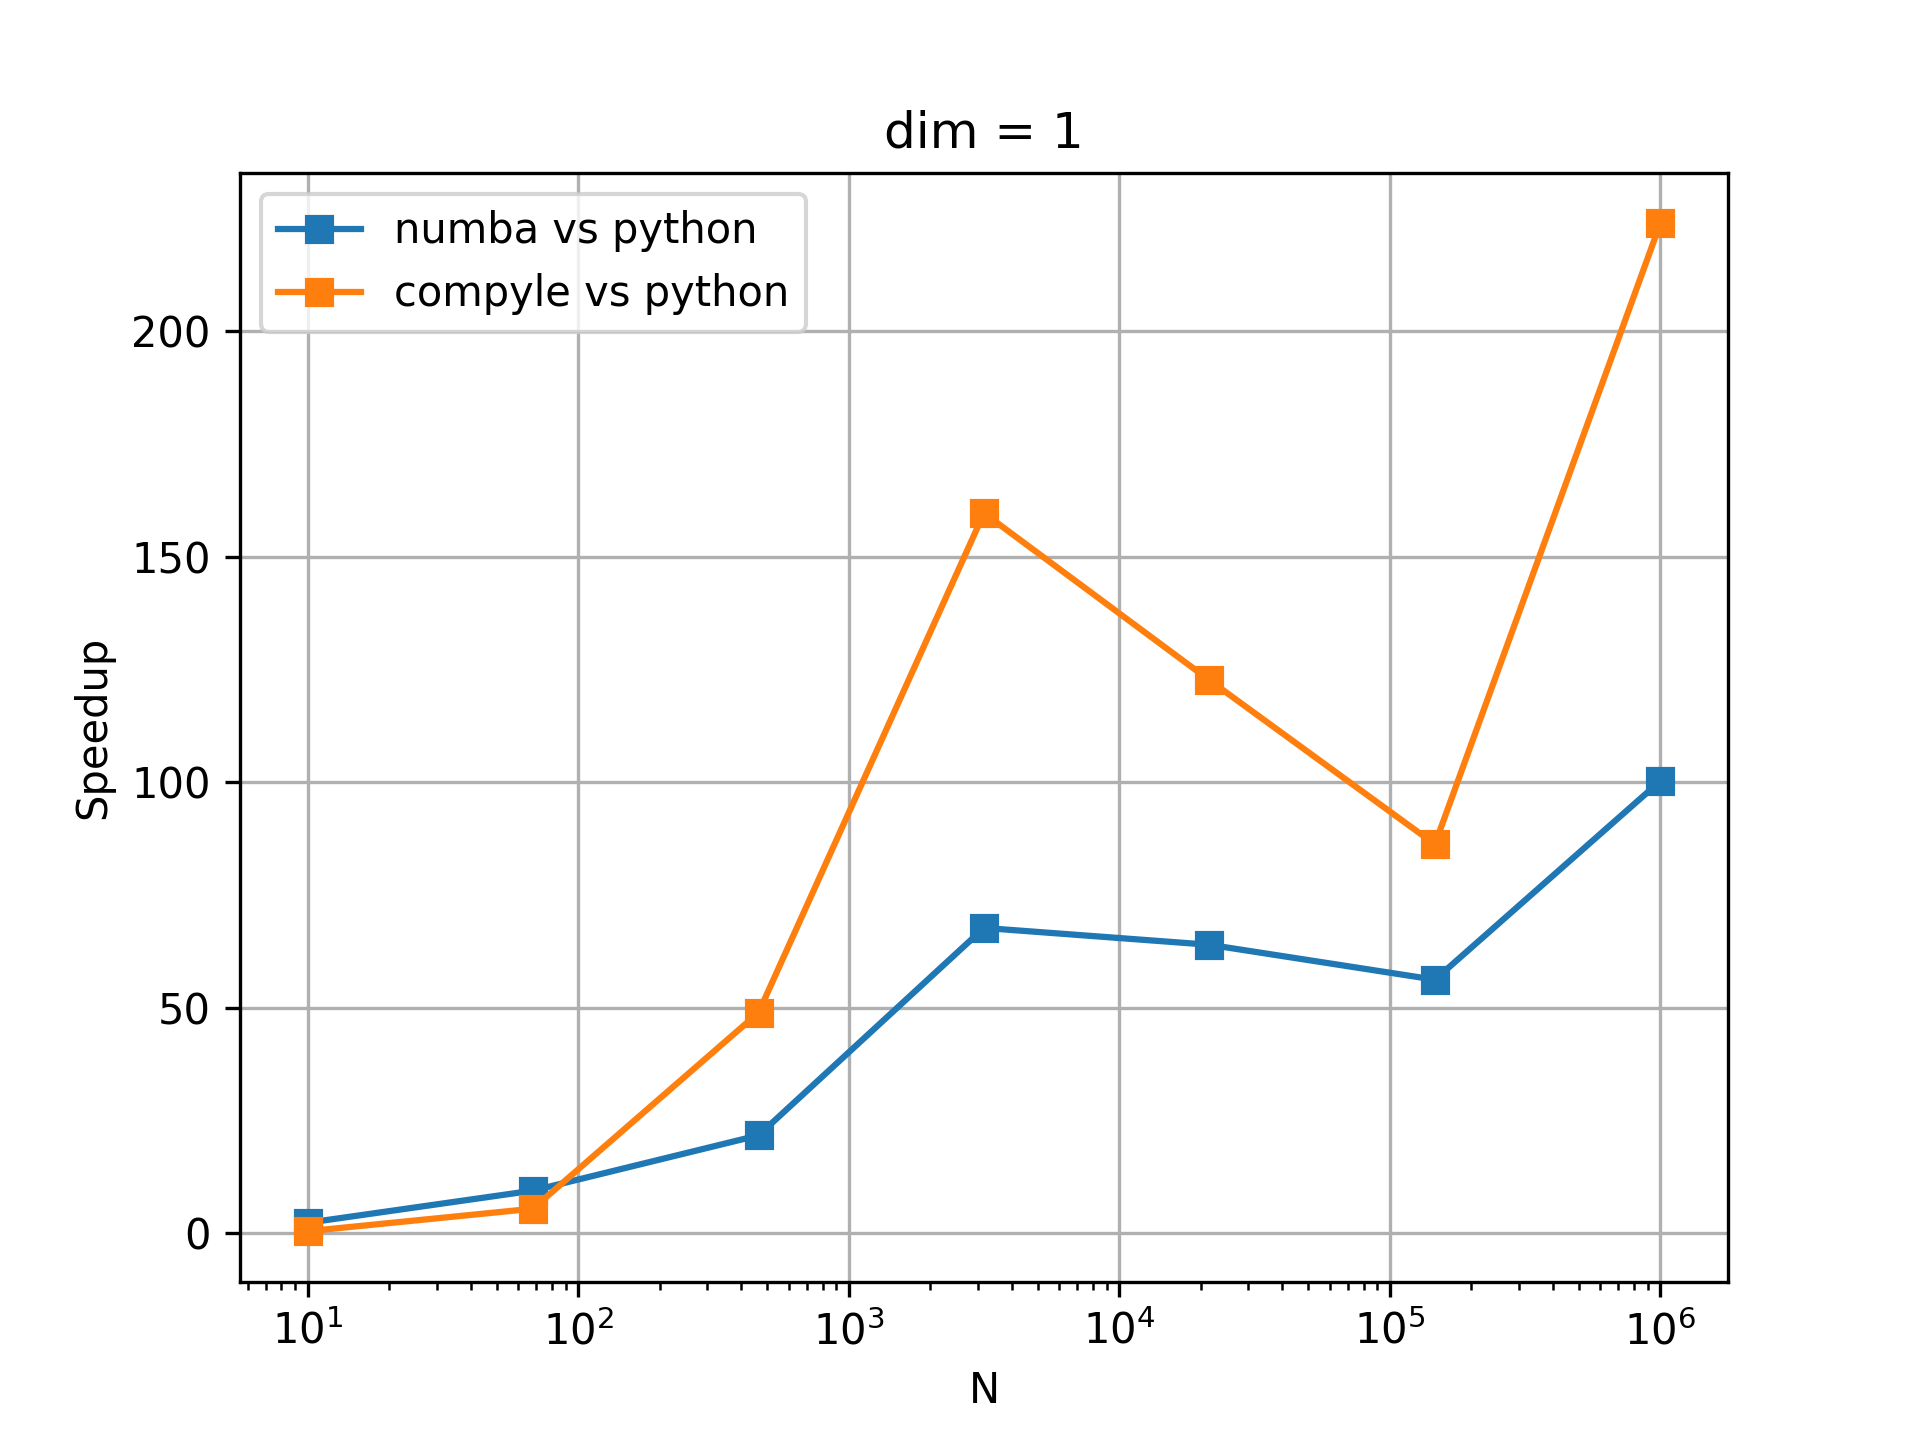
\includegraphics[width=6cm]{Code-Figures/espec_speedup_dim_1.png}
      \caption{$1D$ velocity field}
    \end{subfigure}
    \begin{subfigure}{7cm}
      \centering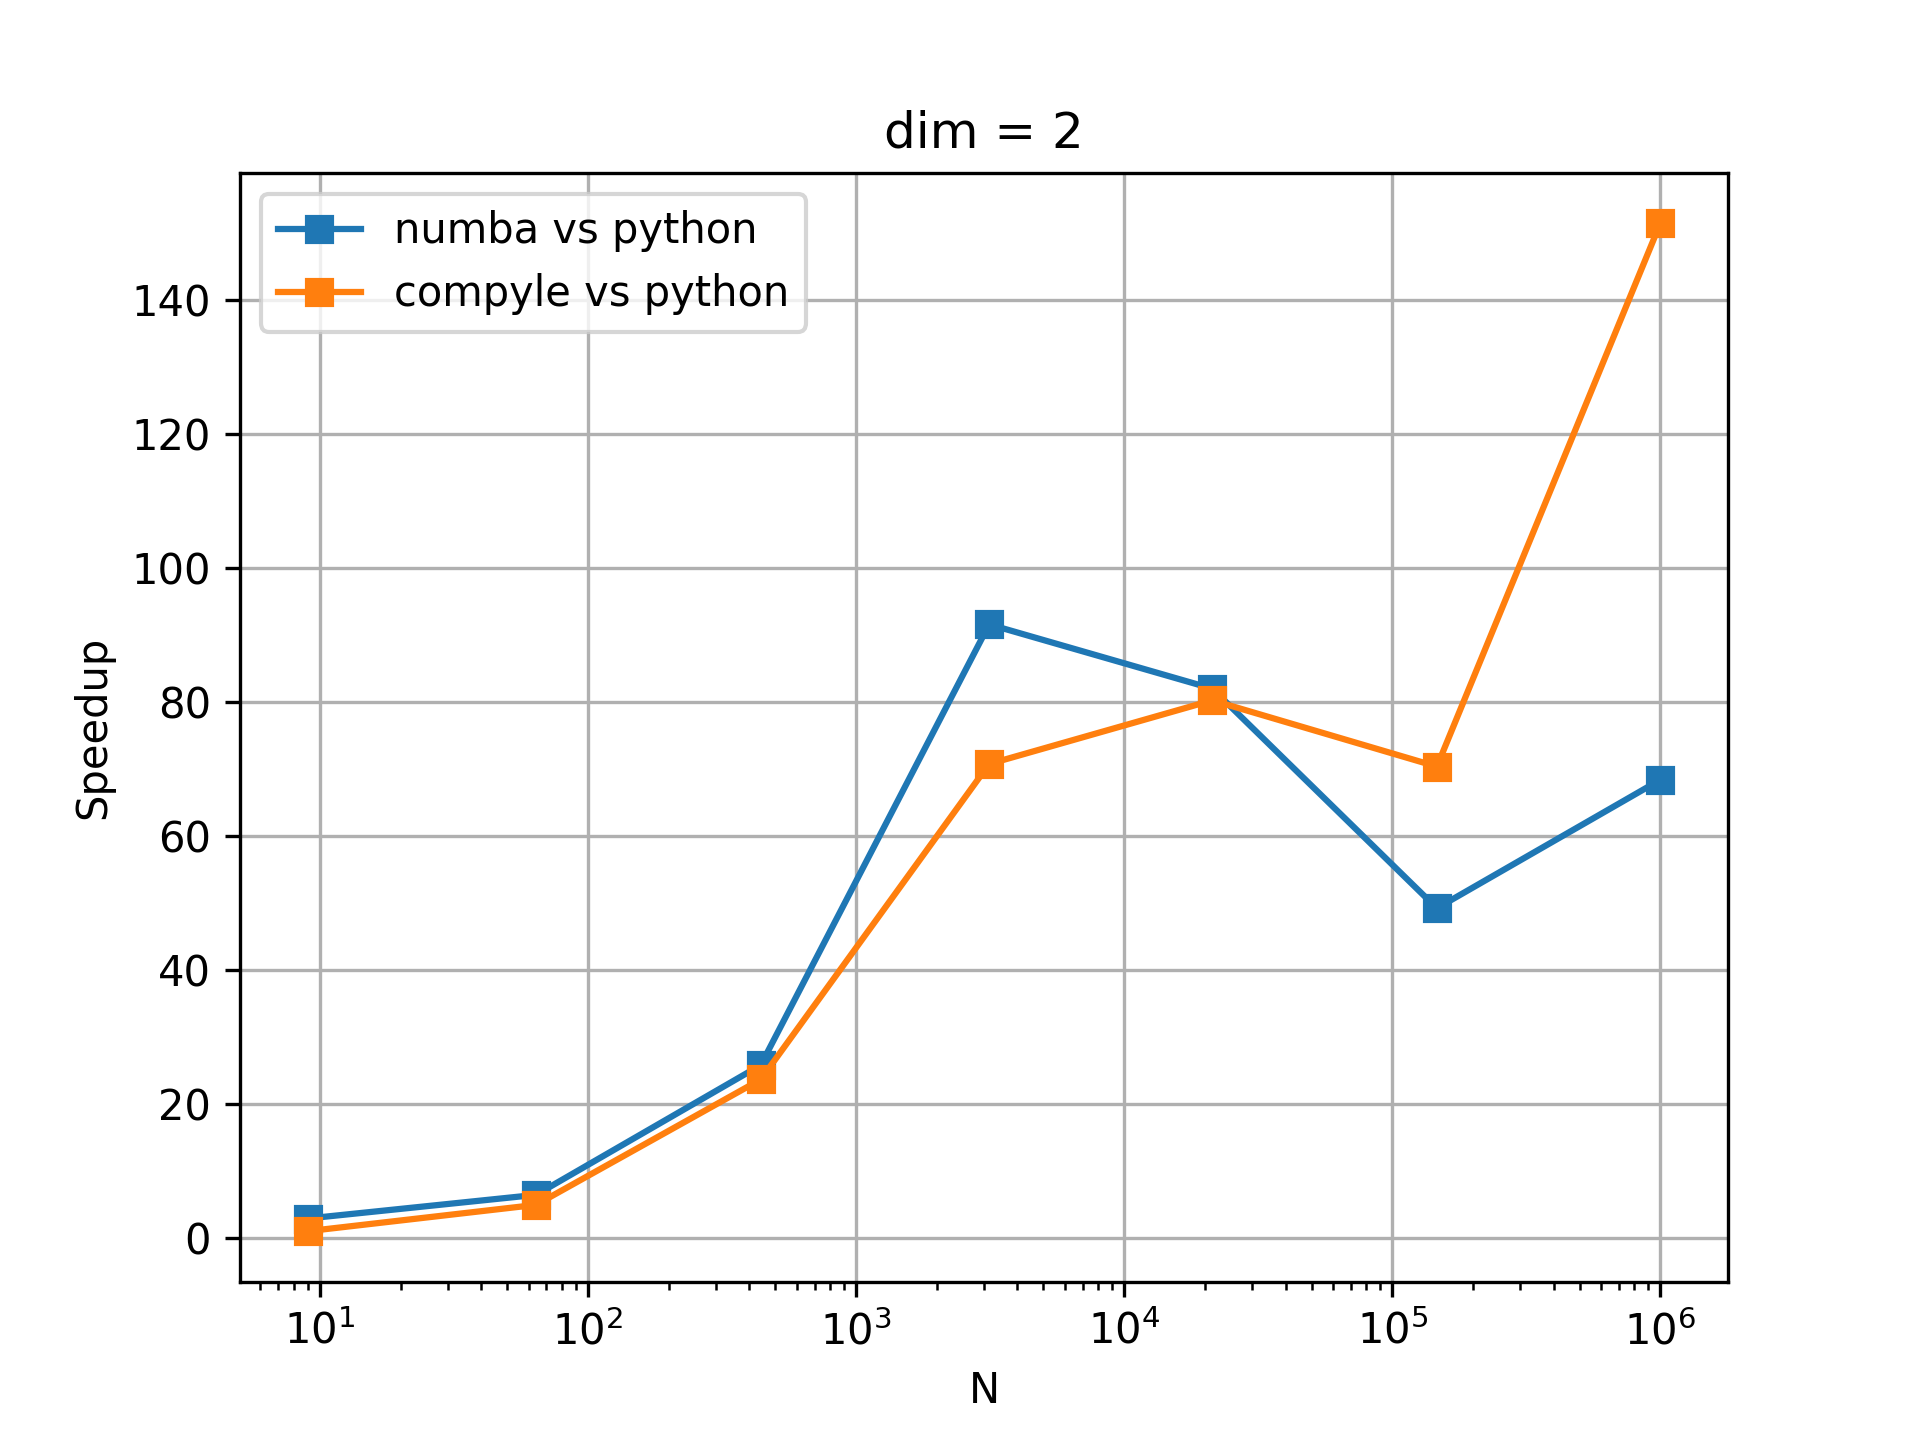
\includegraphics[width=6cm]{Code-Figures/espec_speedup_dim_2.png}
      \caption{$2D$ velocity field}
    \end{subfigure}
    \begin{subfigure}{7cm}
      \centering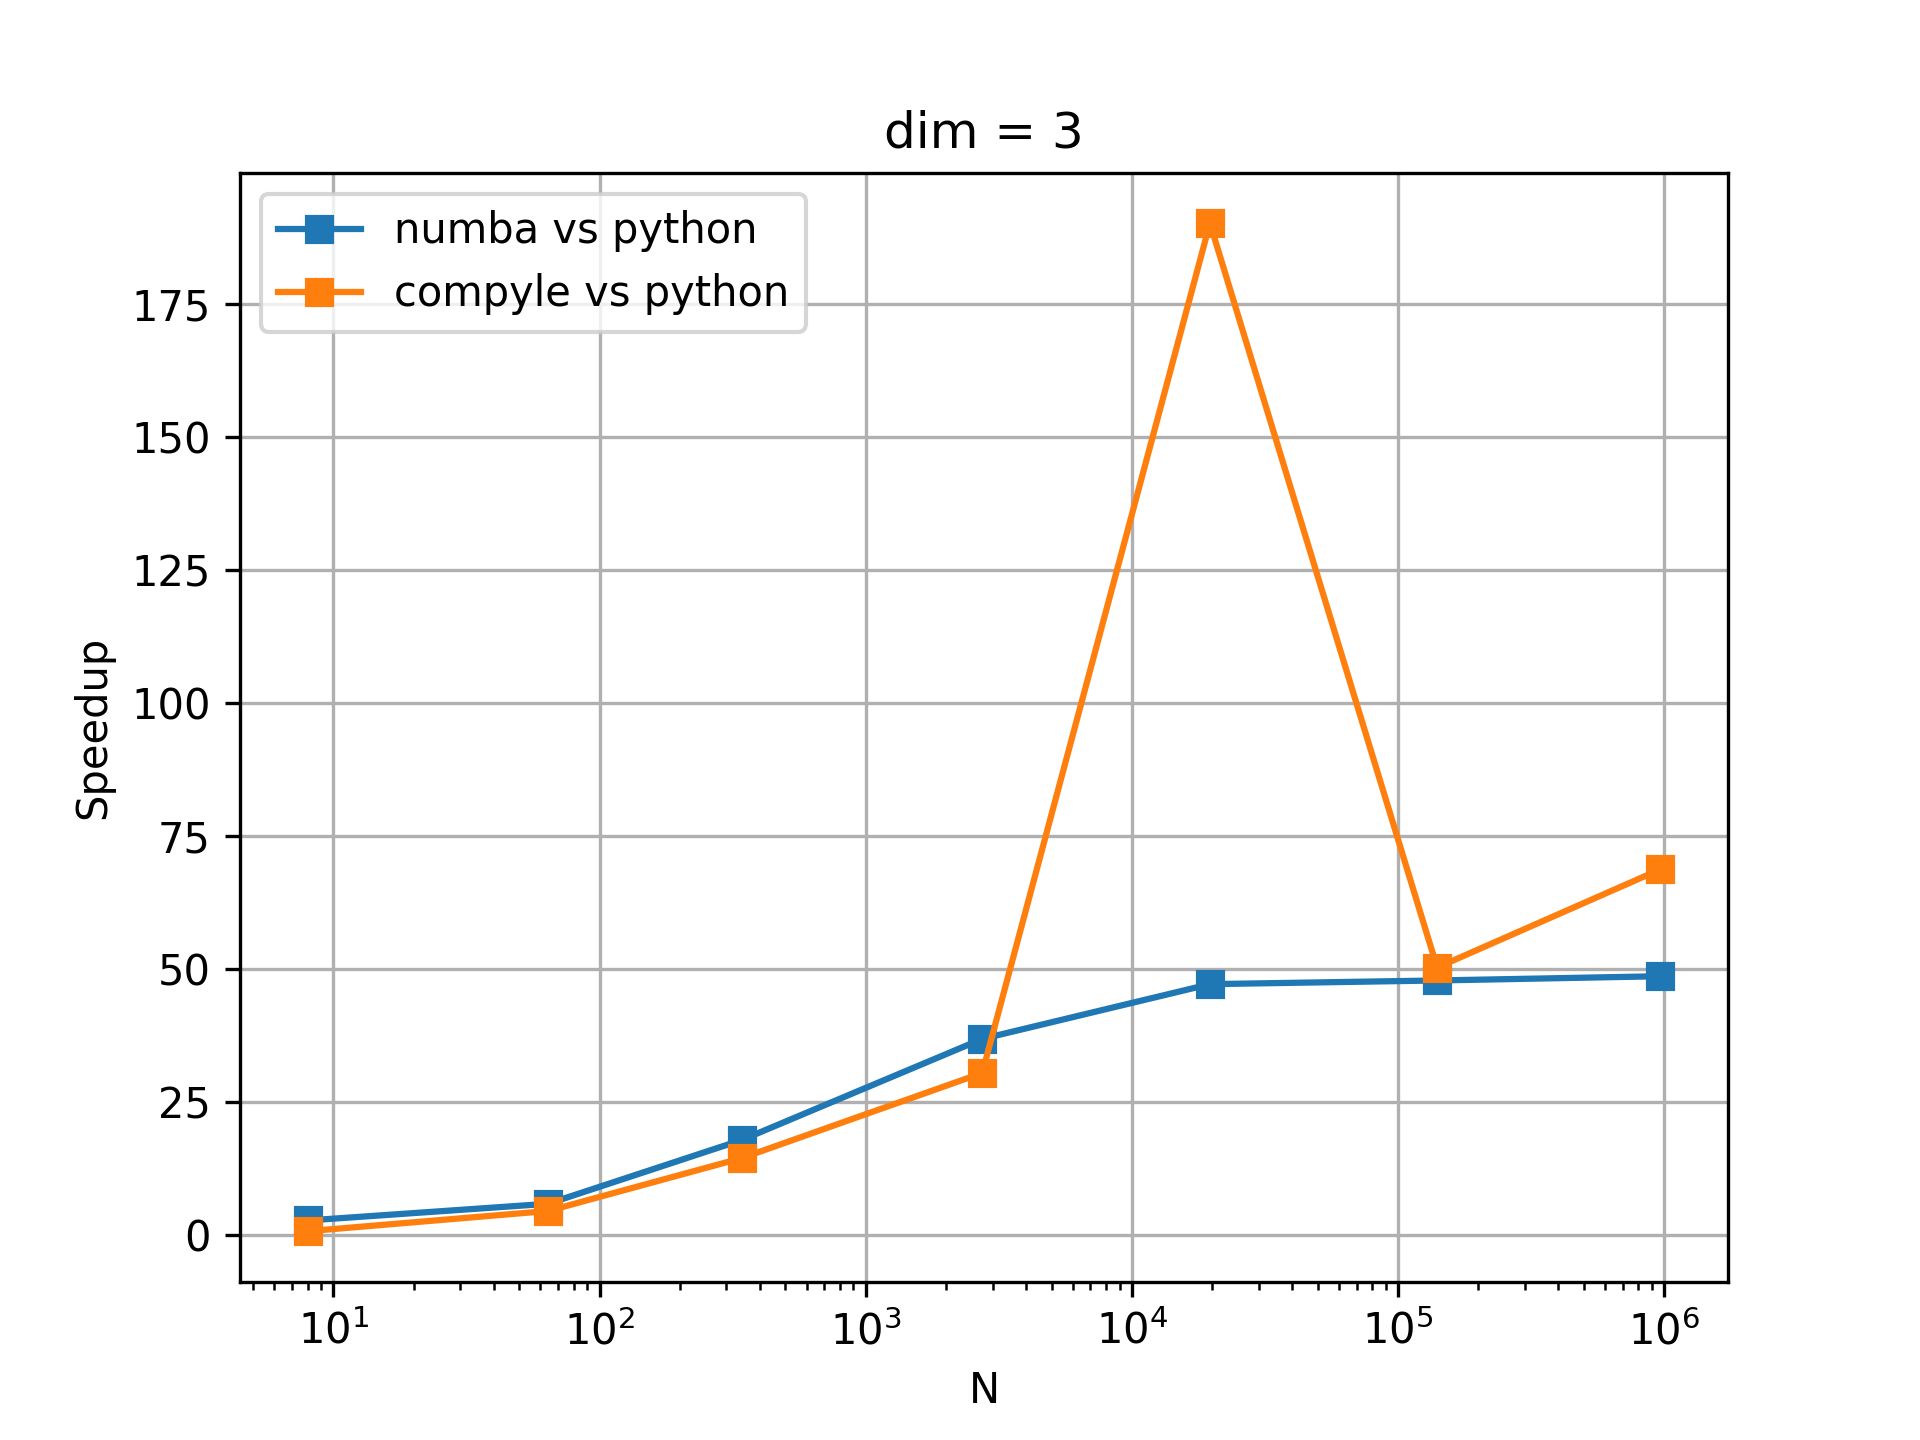
\includegraphics[width=6cm]{Code-Figures/espec_speedup_dim_3.png}
      \caption{$3D$ velocity field}
    \end{subfigure}
    \caption{Speedup of the $1D$ energy spectrum computation for various dimensions of the velocity field.}
    \label{fig:espec-speedup}
\end{figure}

As seen, in the speedup plots, the \texttt{numba} implementation is around $50-100\times$ faster than the pure \texttt{python} implementation, while the \texttt{compyle} implementation is around $80-150\times$ faster than the pure \texttt{python} implementation for various resolution scales. These trends are observed for all the three dimensions of the velocity field. The \texttt{compyle} implementation, in addition to begin faster than the \texttt{numba} implementation, also has the added advantage of not requiring any additional dependencies, which are not already required by \texttt{PySPH}, unlike the \texttt{numba} implementation, which requires the \texttt{numba} package to be installed separately. Hence, the \texttt{compyle} implementation was chosen for the final implementation of the $1D$ energy spectrum computation.

In order to test the code for correctness, the following test-cases were devised. The velocity field for $1D$, is given as:
\begin{equation}
    v_x = - \sum_{i=1}^{N} i^{-\gamma} \cos(2 \pi i x),
\end{equation}
where, $N$ is the number of modes, and $\gamma$ is the decay rate of the modes.
For $2D$, the velocity field is given as:
\begin{equation}
    v_x = - \sum_{i=1}^{N} i^{-\gamma} \cos(2 \pi i x) \sin(2 \pi i y)
\end{equation}
\begin{equation}
    v_y = \sum_{i=1}^{N} i^{-\gamma} \sin(2 \pi i x) \cos(2 \pi i y).
\end{equation}
For $3D$, the velocity field is given as:
\begin{equation}
    v_x = - \sum_{i=1}^{N} i^{-\gamma} \cos(2 \pi i x) \sin(2 \pi i y) \sin(2 \pi i z)
\end{equation}
\begin{equation}
    v_y = \sum_{i=1}^{N} i^{-\gamma} \sin(2 \pi i x) \cos(2 \pi i y) \sin(2 \pi i z)
\end{equation}
\begin{equation}
    v_z = \sum_{i=1}^{N} i^{-\gamma} \sin(2 \pi i x) \sin(2 \pi i y) \cos(2 \pi i z).
\end{equation}
Since the energy in the flow field is a function of the square of the velocity, the corresponding decay rate in the energy spectrum is going to be $2\gamma$.

First order of correctness, involved running the energy spectral calculation for the above test-cases, using only one mode ($N=1$), and zero decay rate ($\gamma=0$).

The vector energy spectral fields are show in \figref{fig:espec-vector-fields-N1}. It should be noted, that the plots are shown by shifting the energy spectrum, such that the center of the plot corresponds to the zero wavenumber. This is done, since the energy spectrum is symmetric about the zero wavenumber, and hence, the plot is more informative when the zero wavenumber is at the center of the plot. Here, it can be observed that in both the $1D$ and $2D$ case the energy spectrum peaks only for $k=1$, and is zero for every other wavenumber, indicating the nature of the velocity field, consisting of only one mode. 

The scalar energy spectral fields are shown in \figref{fig:espec-scalar-fields-N1}. As can be seen, the energy spectrum peaks only for $k=1$, and is zero for every other wavenumber for all dimensions.

\begin{figure}[H]
    \begin{subfigure}{7cm}
      \centering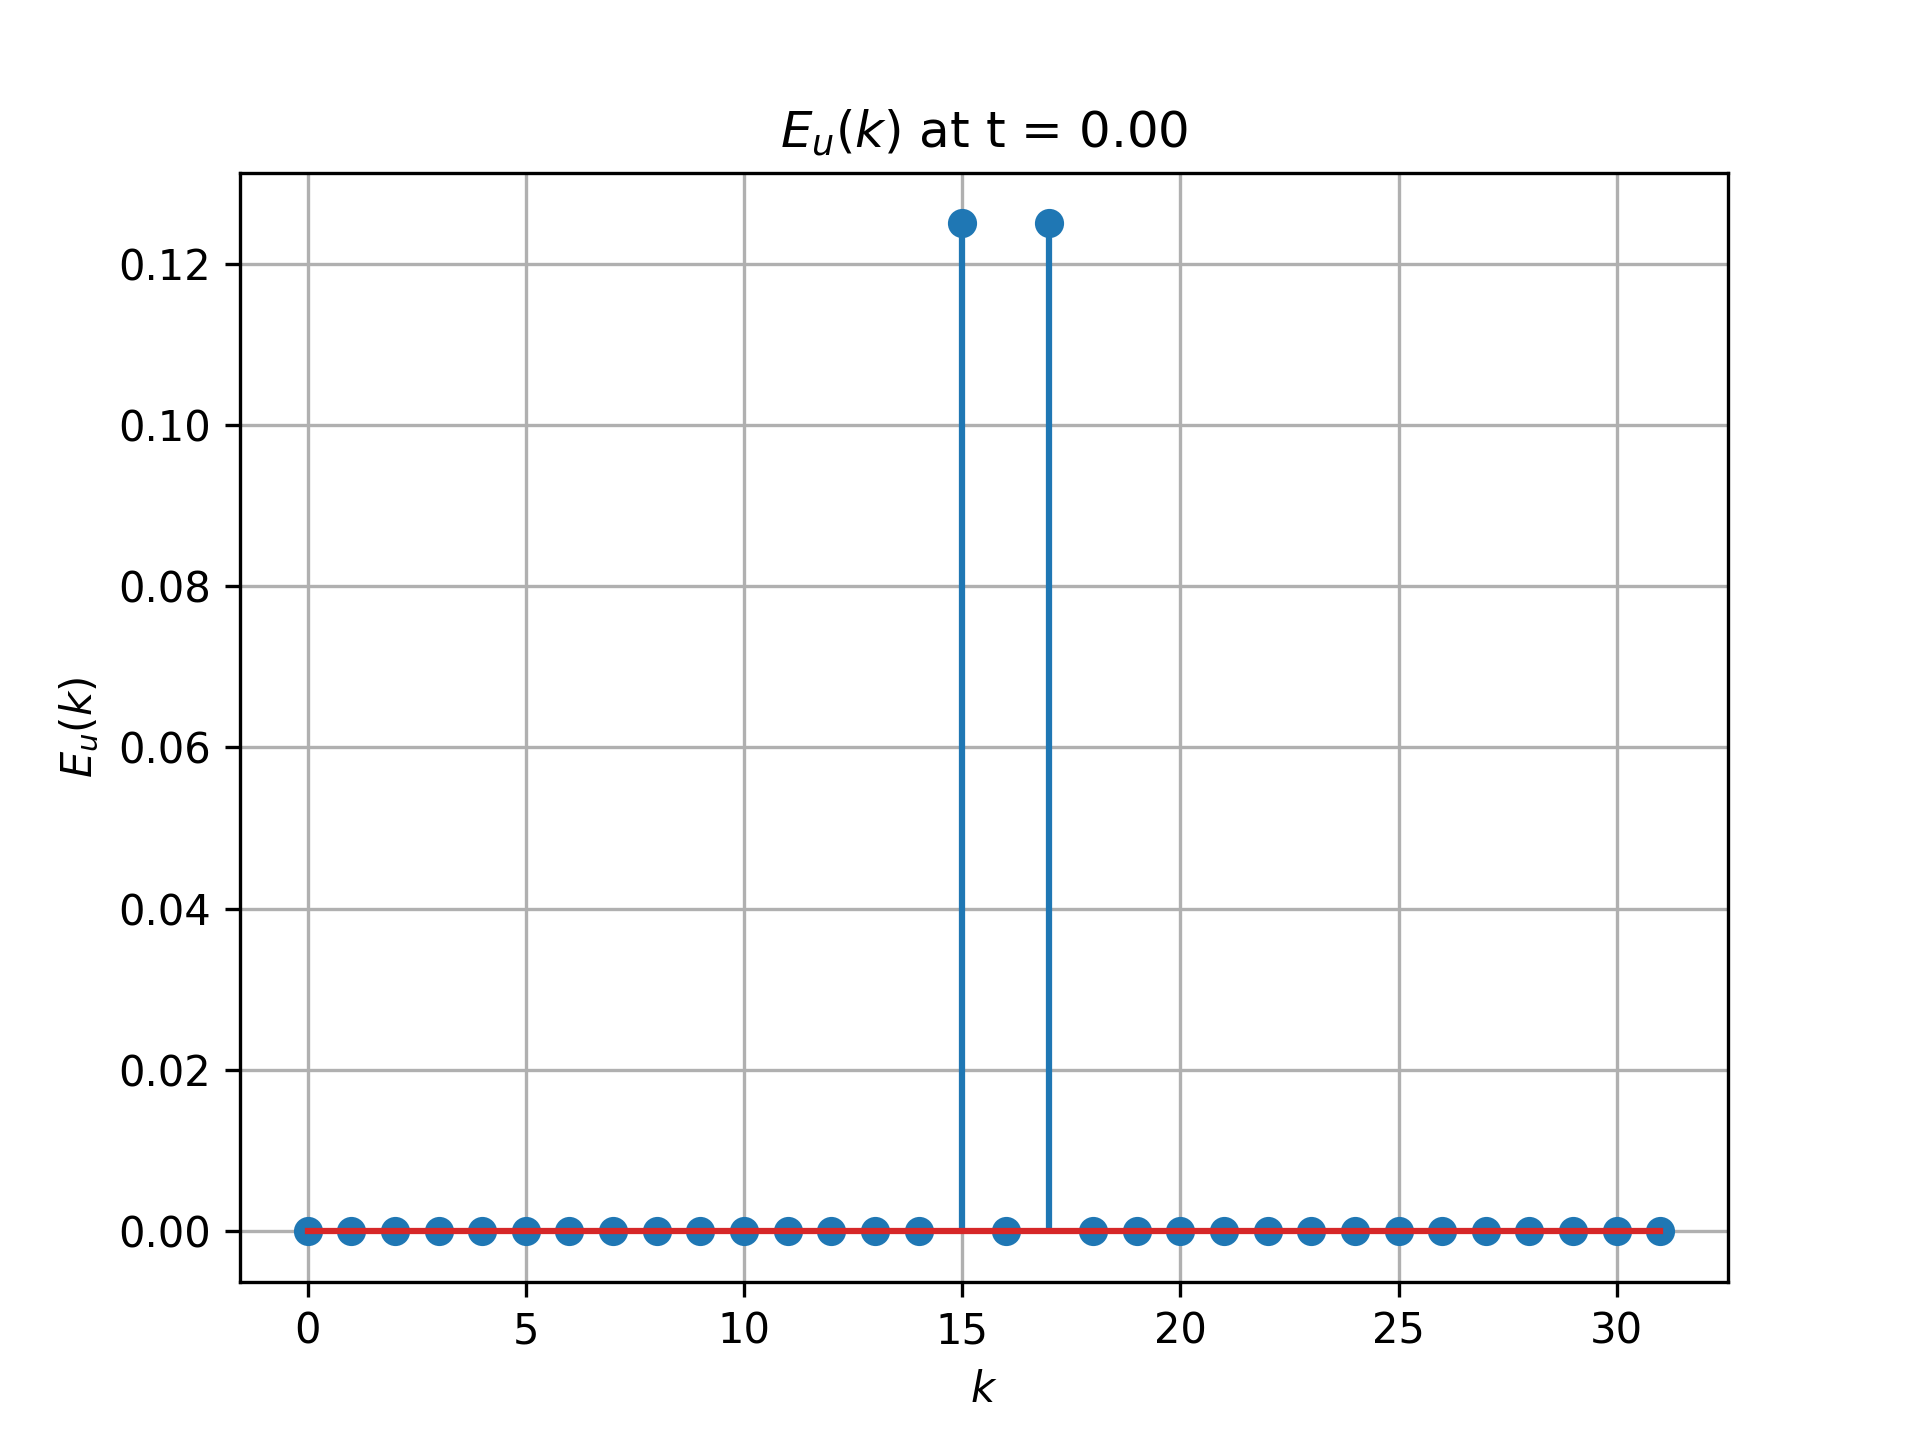
\includegraphics[width=6cm]{Code-Figures/espec-simple-1d/EK_spectrum.png}
      \caption{$1D$ $\vect{E}(\vect{k})$ field}
    \end{subfigure}
    \begin{subfigure}{7cm}
      \centering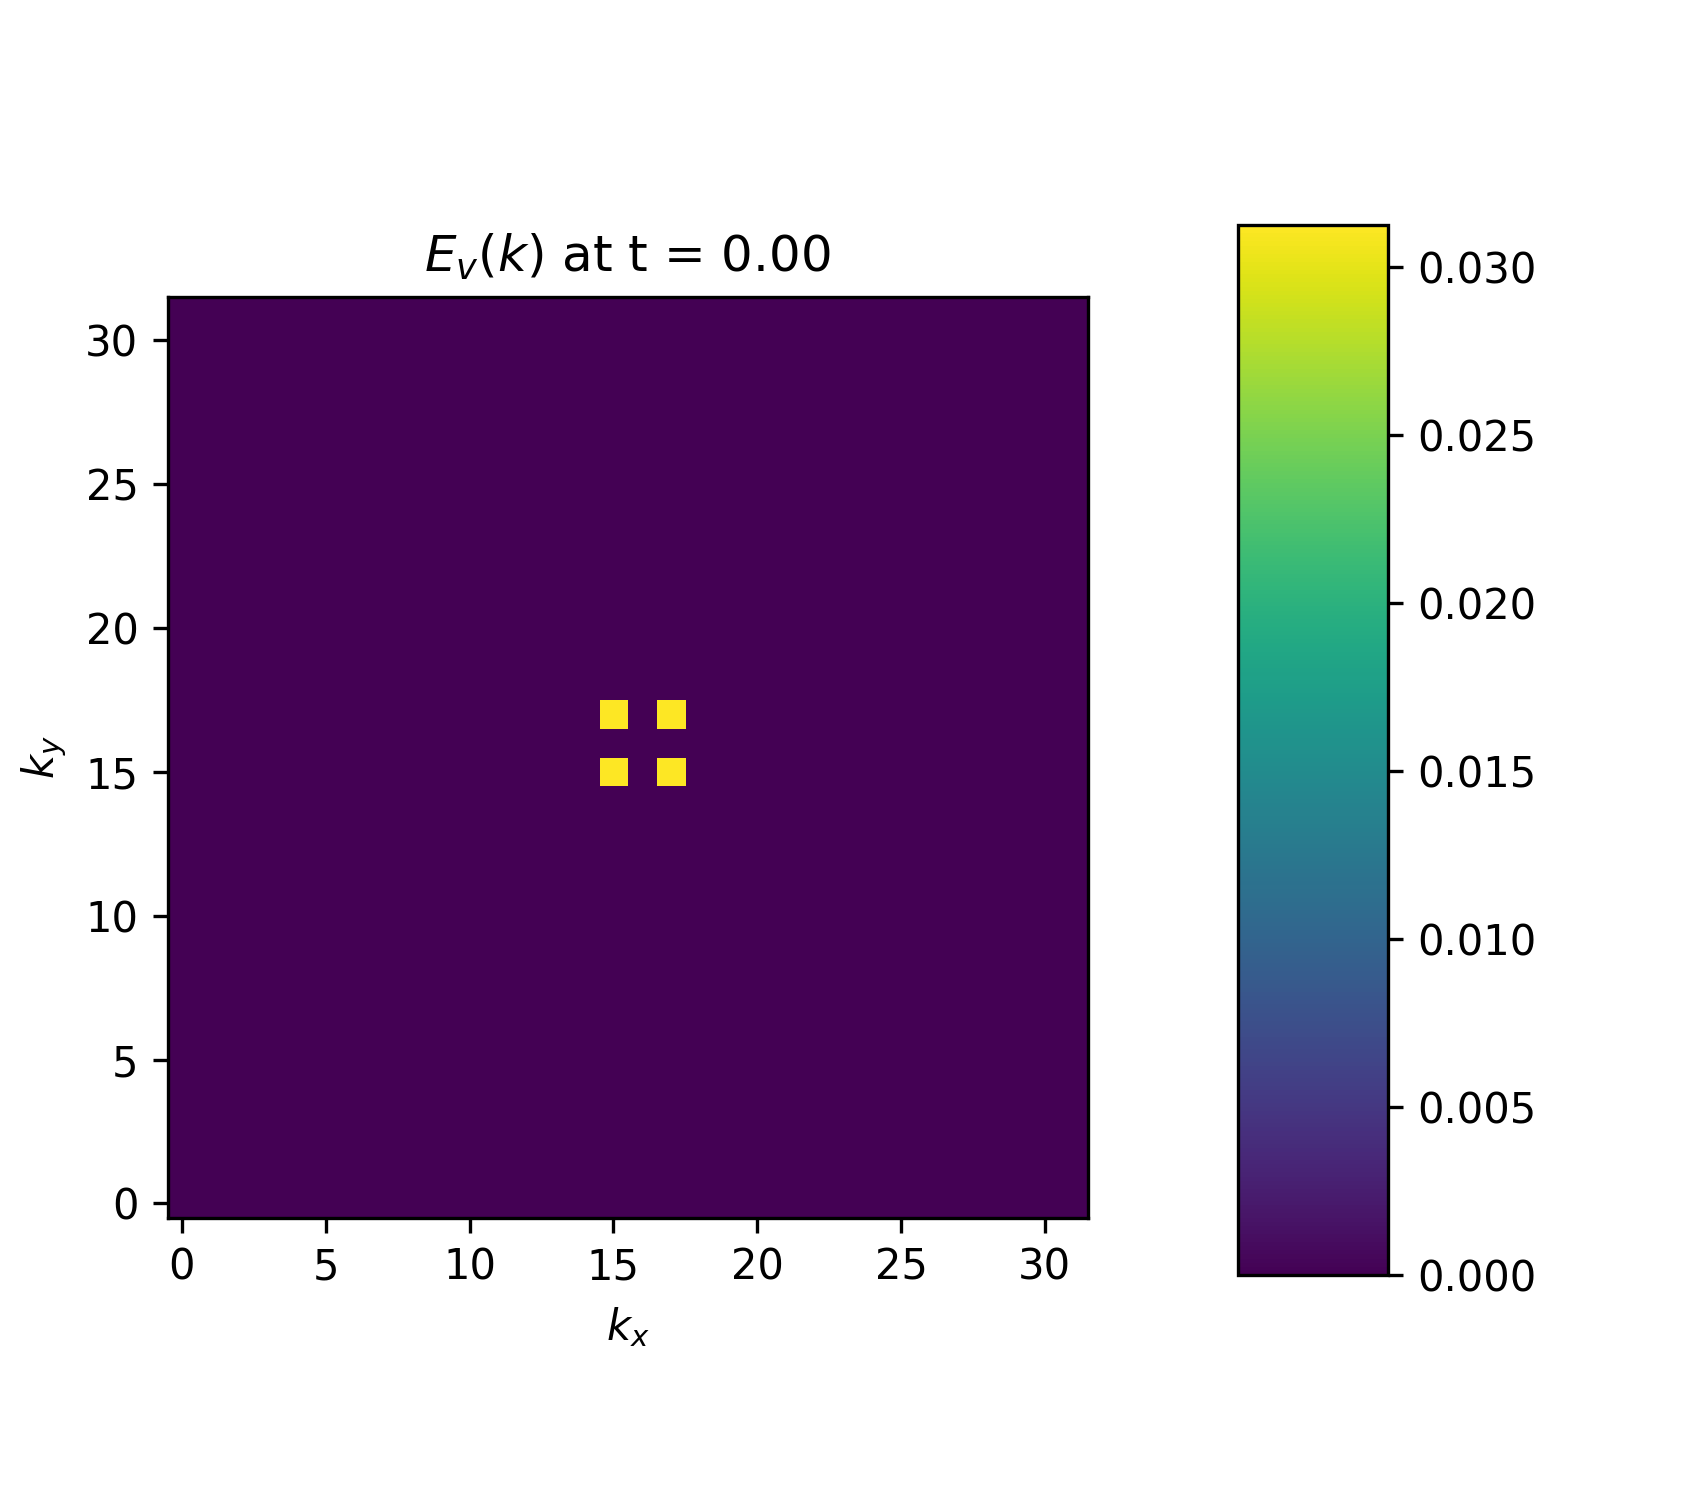
\includegraphics[width=6cm]{Code-Figures/espec-simple-2d/EK_spectrum.png}
      \caption{$2D$ $\vect{E}(\vect{k})$ field}
    \end{subfigure}
    \caption{The vector fields $\vect{E}(\vect{k})$ for $1D$ and $2D$ case, with decay rate $\gamma=0$, and $N=1$.}
    \label{fig:espec-vector-fields-N1}
\end{figure}

\begin{figure}[H]
    \begin{subfigure}{7cm}
      \centering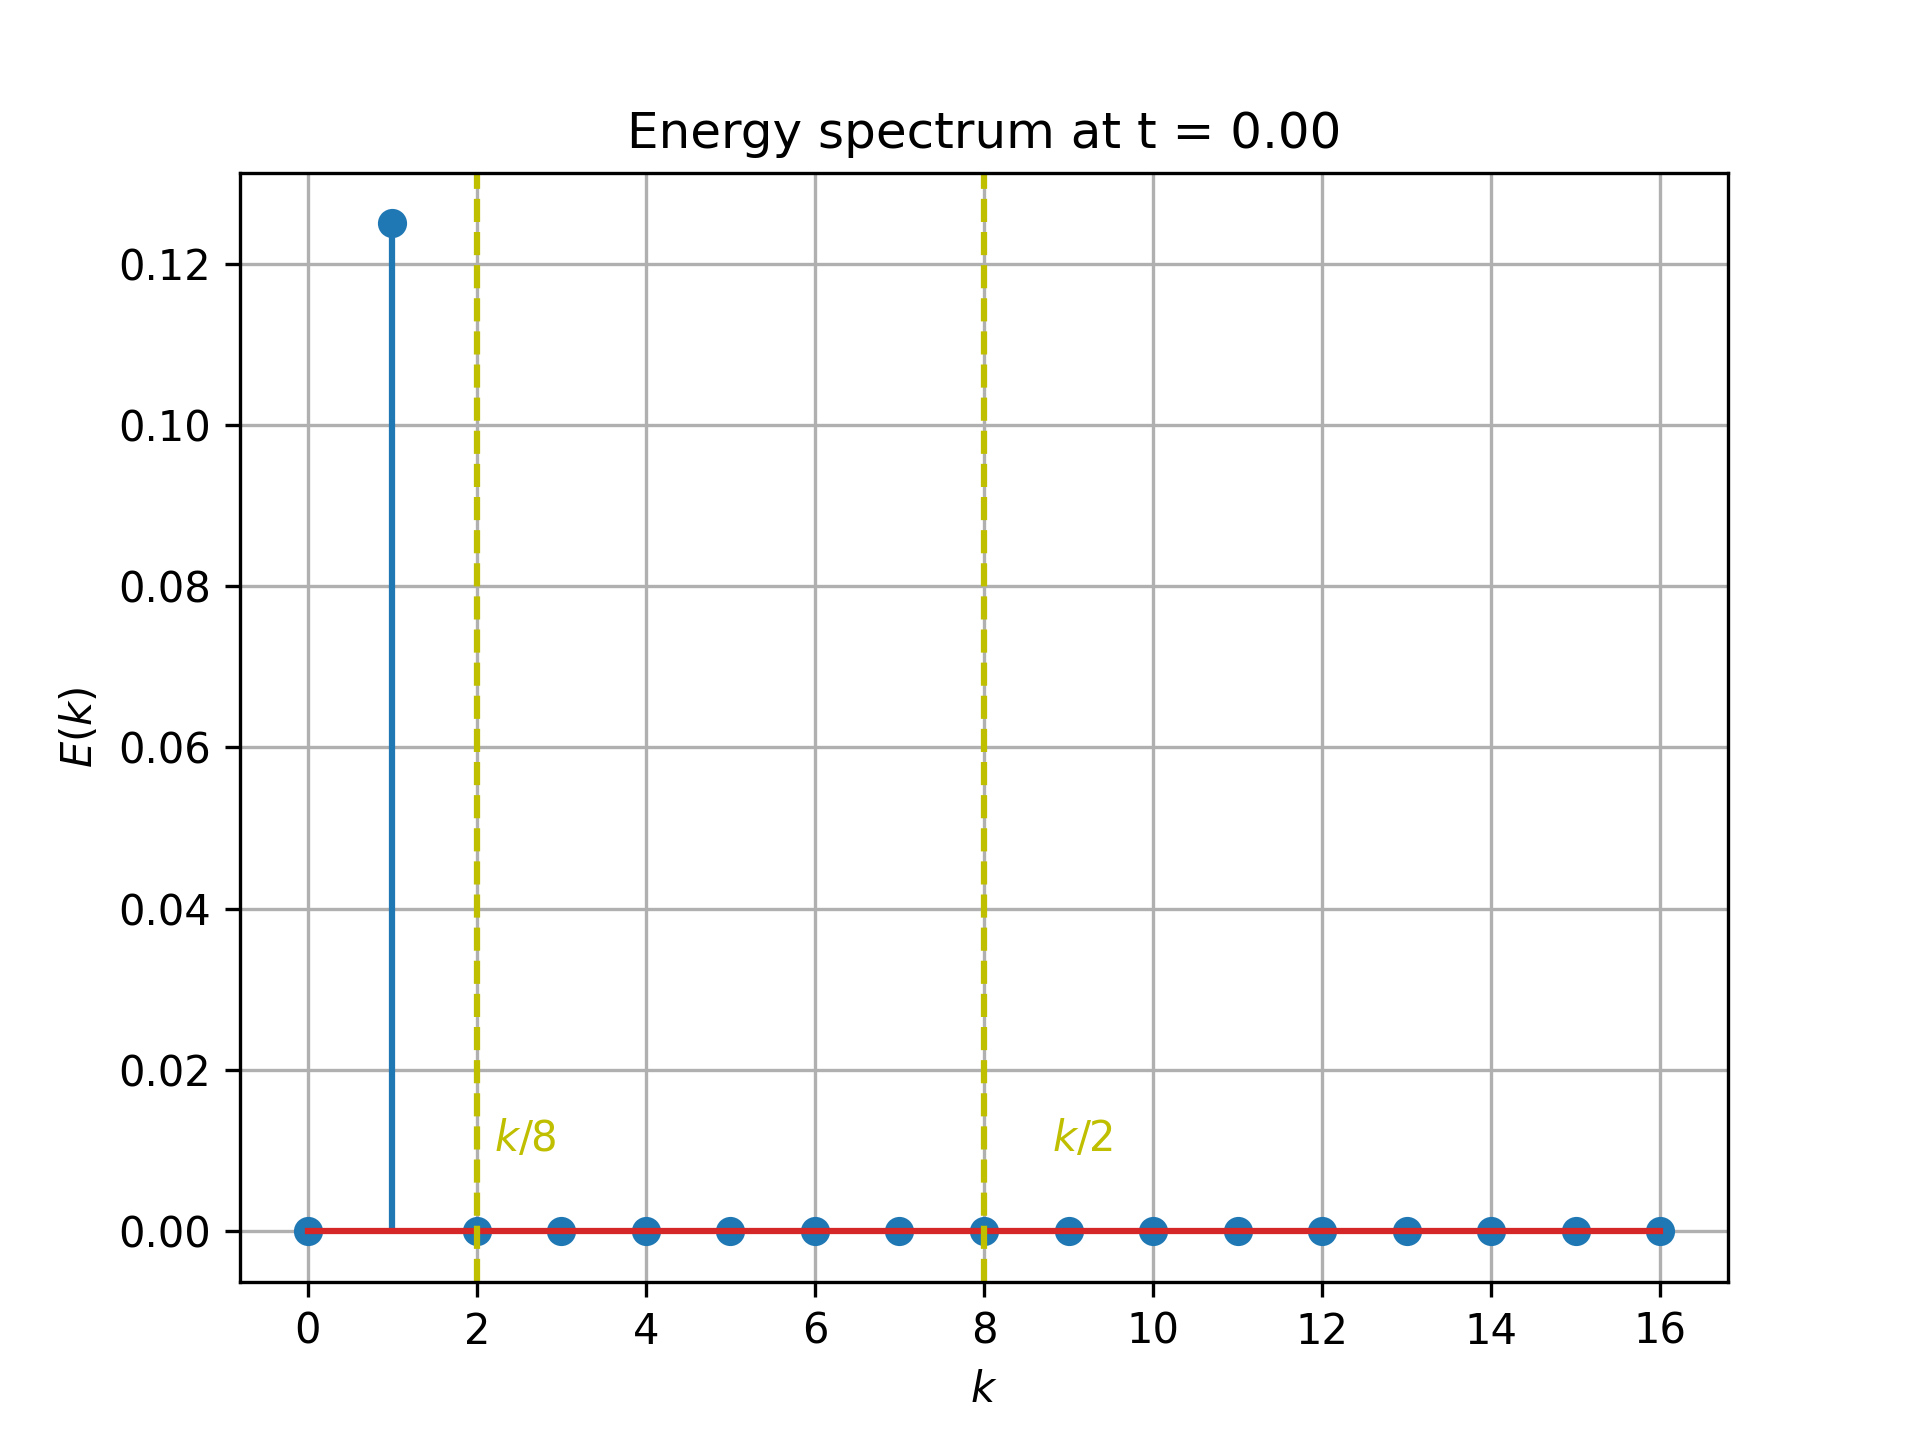
\includegraphics[width=6cm]{Code-Figures/espec-simple-1d/energy_spectrum.png}
      \caption{$1D$ $E(k)$ field}
    \end{subfigure}
    \begin{subfigure}{7cm}
      \centering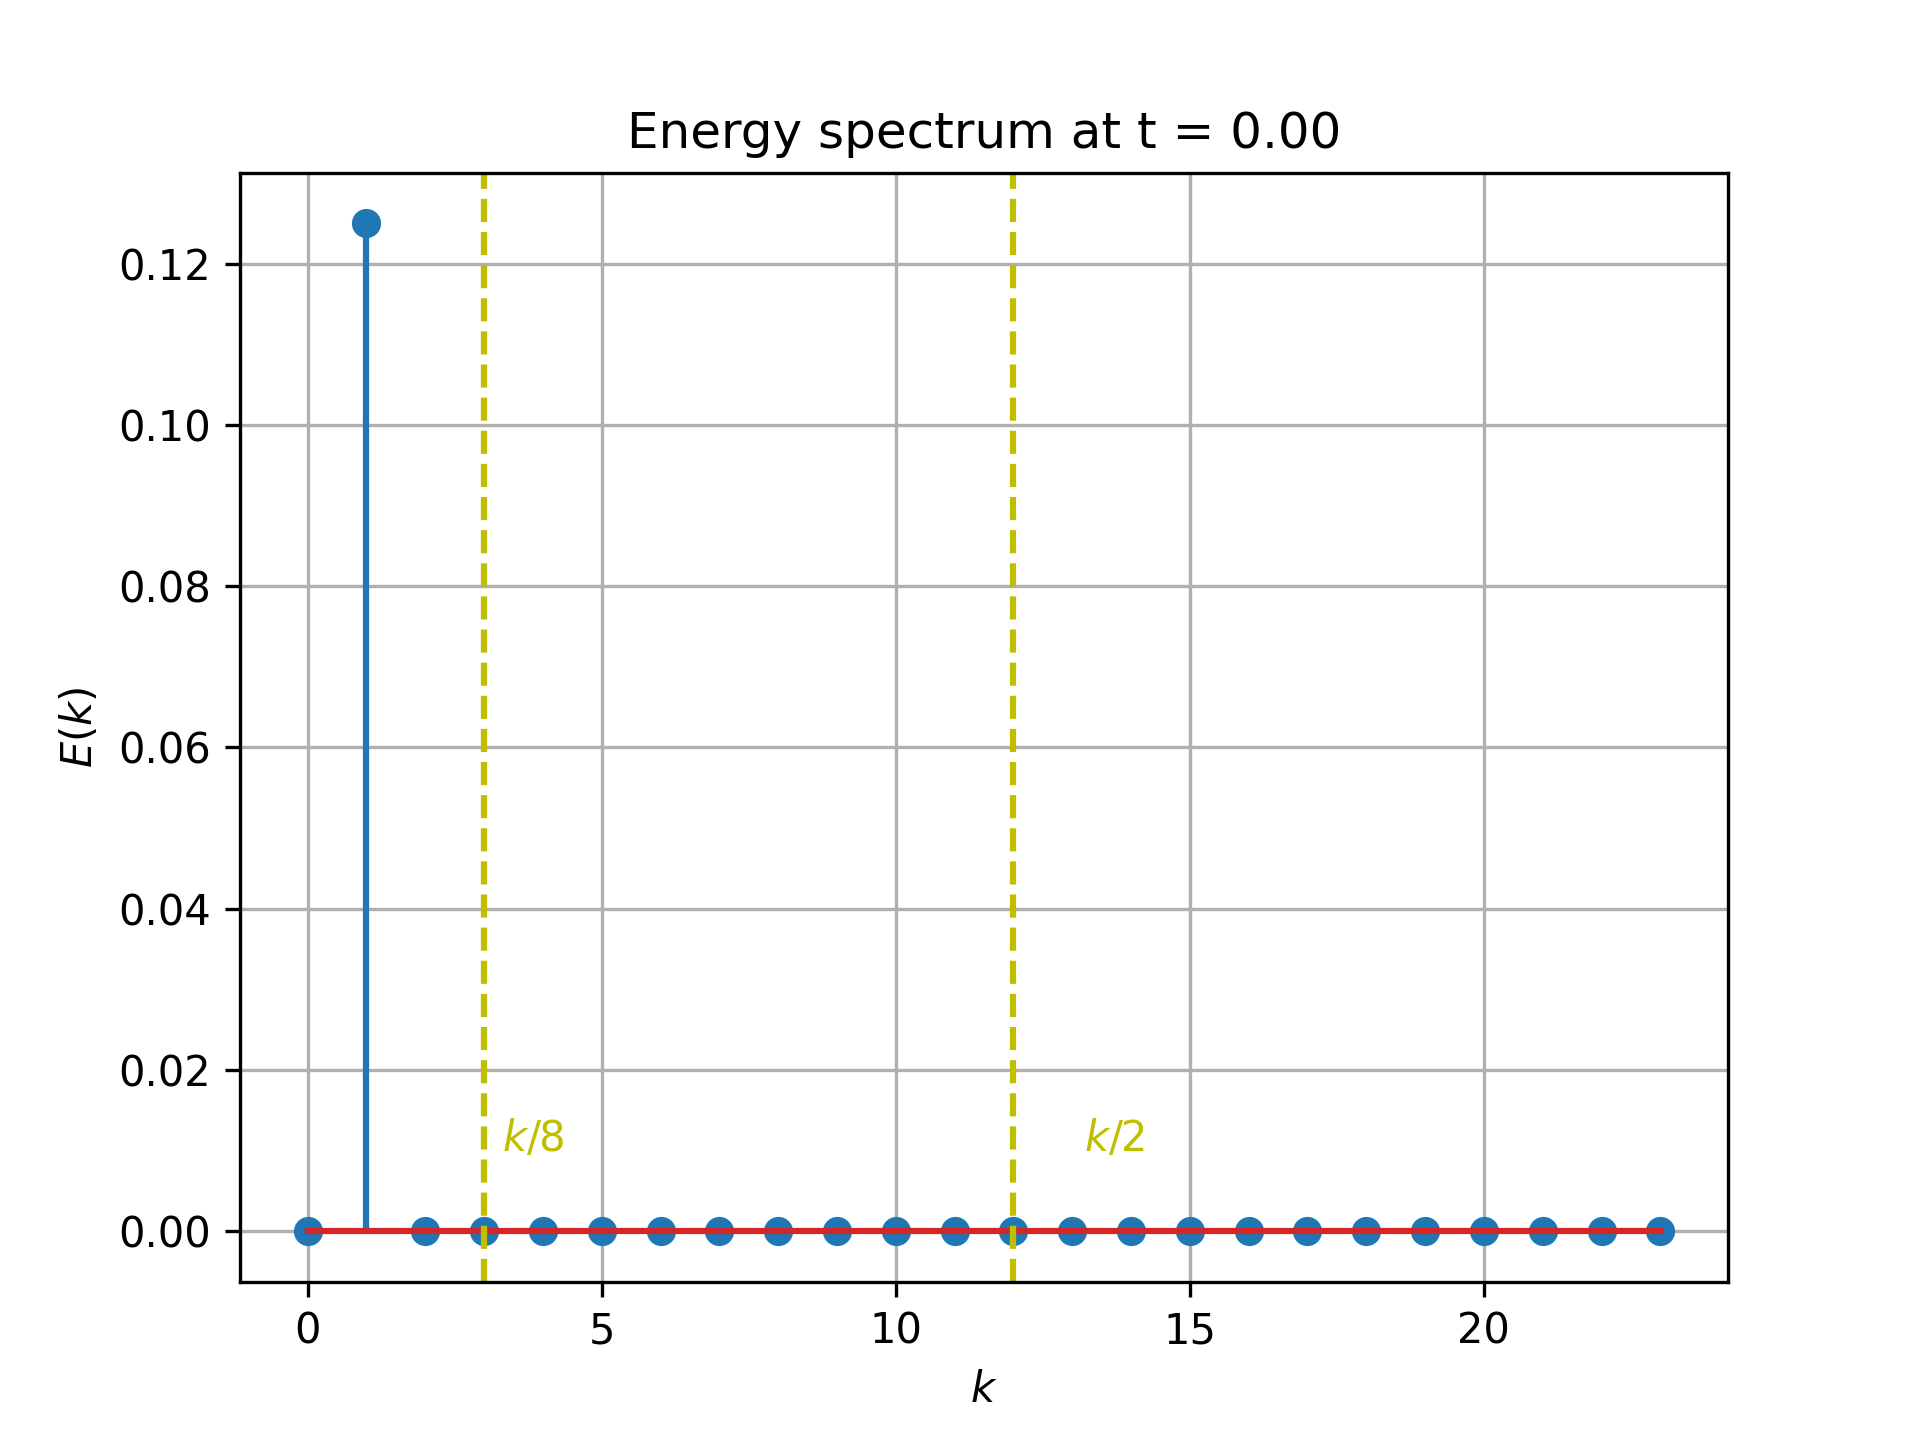
\includegraphics[width=6cm]{Code-Figures/espec-simple-2d/energy_spectrum.png}
      \caption{$2D$ $E(k)$ field}
    \end{subfigure}
    \begin{subfigure}{7cm}
        \centering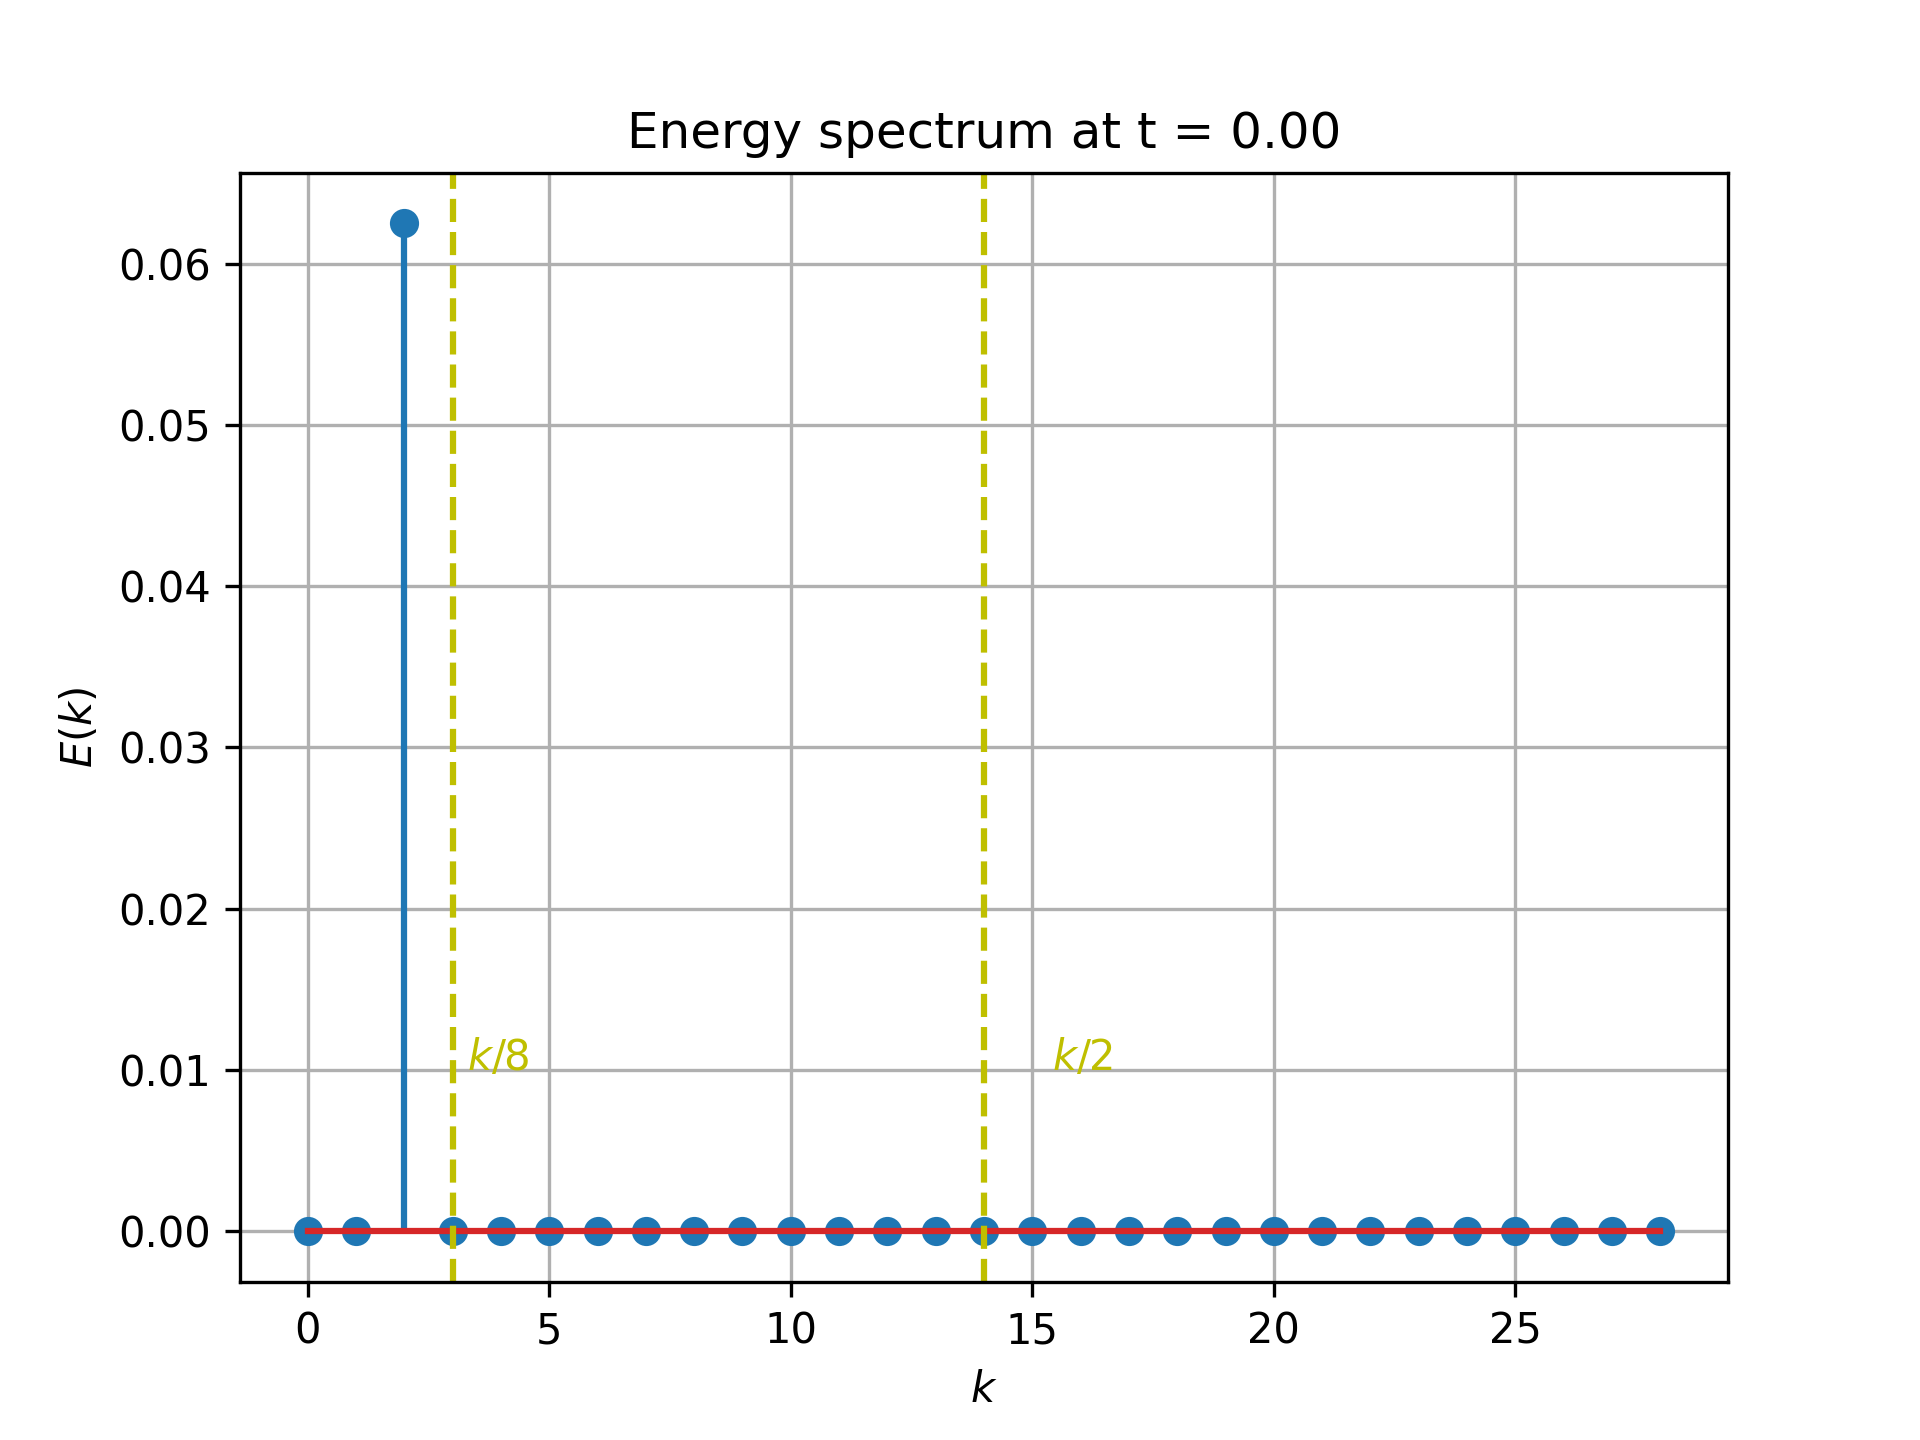
\includegraphics[width=6cm]{Code-Figures/espec-simple-3d/energy_spectrum.png}
        \caption{$3D$ $E(k)$ field}
      \end{subfigure}
    \caption{The scalar fields $E(k)$ for $1D$, $2D$, and $3D$ case, with decay rate $\gamma=0$, and $N=1$.}
    \label{fig:espec-scalar-fields-N1}
\end{figure}

Subsequently, to test the correctness when multiple modes are involved, the test-cases were reconsidered, with $\gamma=1$, and $N$ equal to half the number of particles along one axis of the problem.

The vector energy spectral fields are show in \figref{fig:espec-vector-fields-gamma1}. Here, it can be observed that in both the $1D$ and $2D$ case the energy spectrum peaks for $k=1$, and is non-zero upto $k=n_x/2$, indicating the nature of the velocity field, consisting of multiple modes. The amplitudes are also observed to have an exponential drop-off, as is expected given the nature of the amplitude weigthing.

This is made all the more clear, with the scalar energy spectral fields shown in \figref{fig:espec-scalar-fields-gamma1}. The log-log plots here, allow for the exponential drop-off to be observed more clearly, by fitting a straight line to the log-log plot between wavenumbers $k \in [1, n_x/4]$. The gree-dashed lines which represent the scalar energy spectrum computed for the original velocity field (which is uniform, and rectangular) without interpolation, represents the `best'-case scenario, where the energy spectrum is computed without any loss of information in the velocity field, and the source of noise can be solely attributed to numerical errors from the discrete Fourier transform. The actual scalar energy spectrum computed from the interpolated velocity is plotted in blue.

It is oberseved that energy spectrum computed without interpolation, is indeed the `best'-case scenario, since it much more closely follows the exact trend. However, with the computed energy spectrum from the interpolated velocity field, the trend is still observed to be followed, but only upto the $k/8$ wavenumber, beyond which the trend is lost, and the computed energy spectrum is observed to be much lower than the green-dashed line, with the difference increasing with the wavenumber.
This seems to indicate that the act of interpolation itself, is introducing some amount of noise in the velocity field, which is reflected by the jagged nature of the blue line, and also seems to decrease the energy at lower scales, which is reflected by the blue line being consistently lower than the green-dashed line at lower wavenumbers. This allows for the conclusion that the interpolation scheme, seems to behave as a low-pass filter, which is expected, since the interpolation scheme is essentially a convolution of the velocity field with the kernel function, which is a low-pass filter.

Therefore, it was concluded that the $1D$ energy field, computed from the interpolated velocity field, typically will underestimate the energy at higher wavenumbers, and hence, the slope of the energy spectrum computed from the interpolated velocity field, will be lower than the slope of the energy spectrum computed from the original velocity field, as reflected in \figref{fig:espec-scalar-fields-gamma1} as well.

\begin{figure}[H]
    \begin{subfigure}{7cm}
      \centering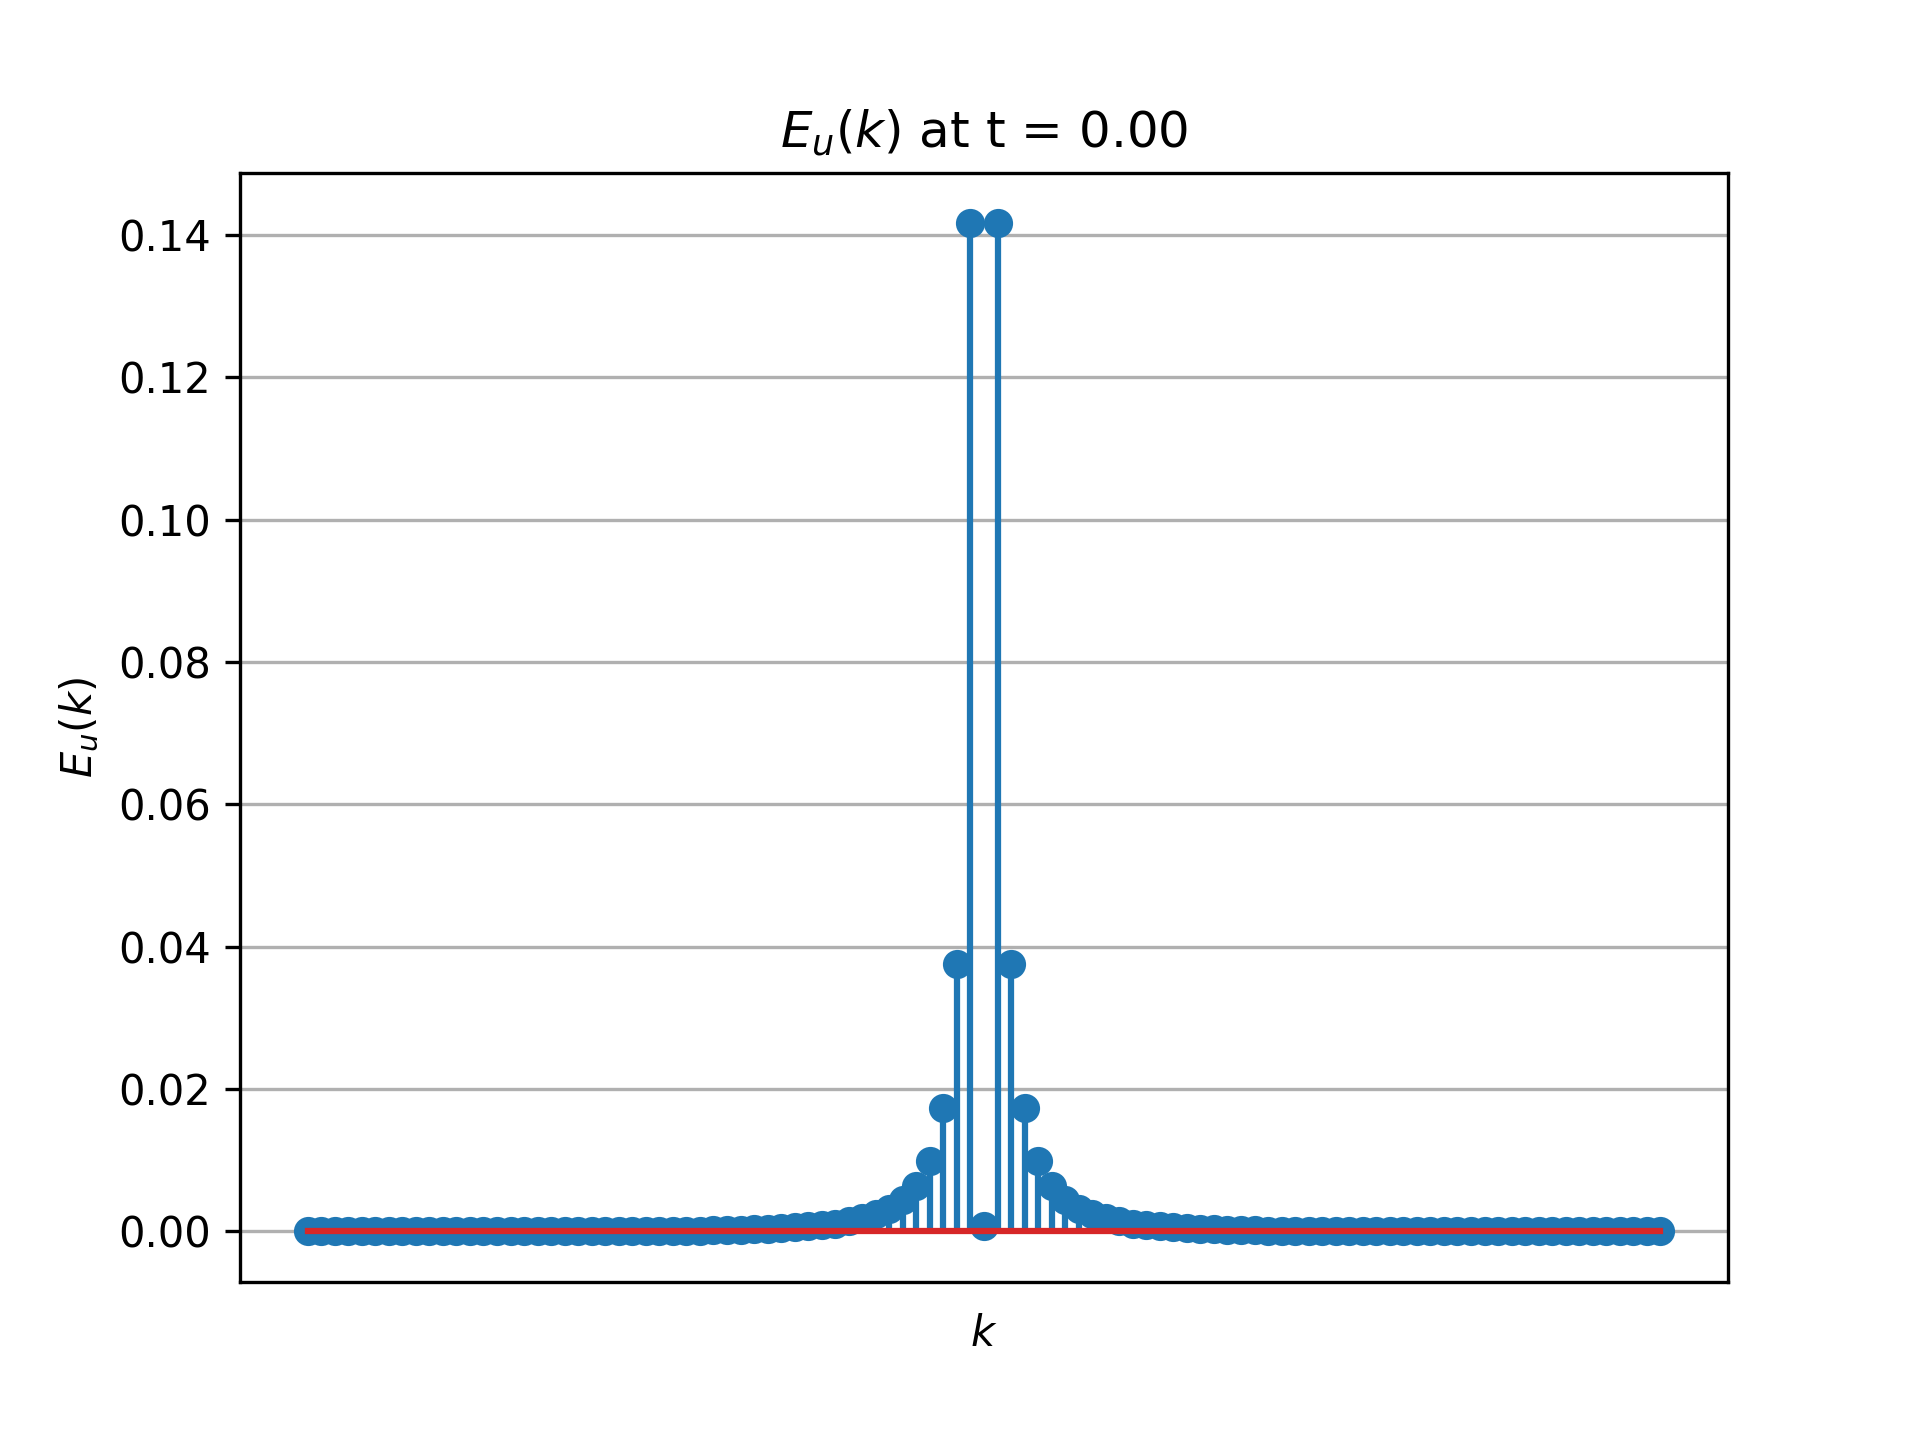
\includegraphics[width=6cm]{Code-Figures/sine-vel-prof-1d/EK_spectrum.png}
      \caption{$1D$ $\vect{E}(\vect{k})$ field}
    \end{subfigure}
    \begin{subfigure}{7cm}
      \centering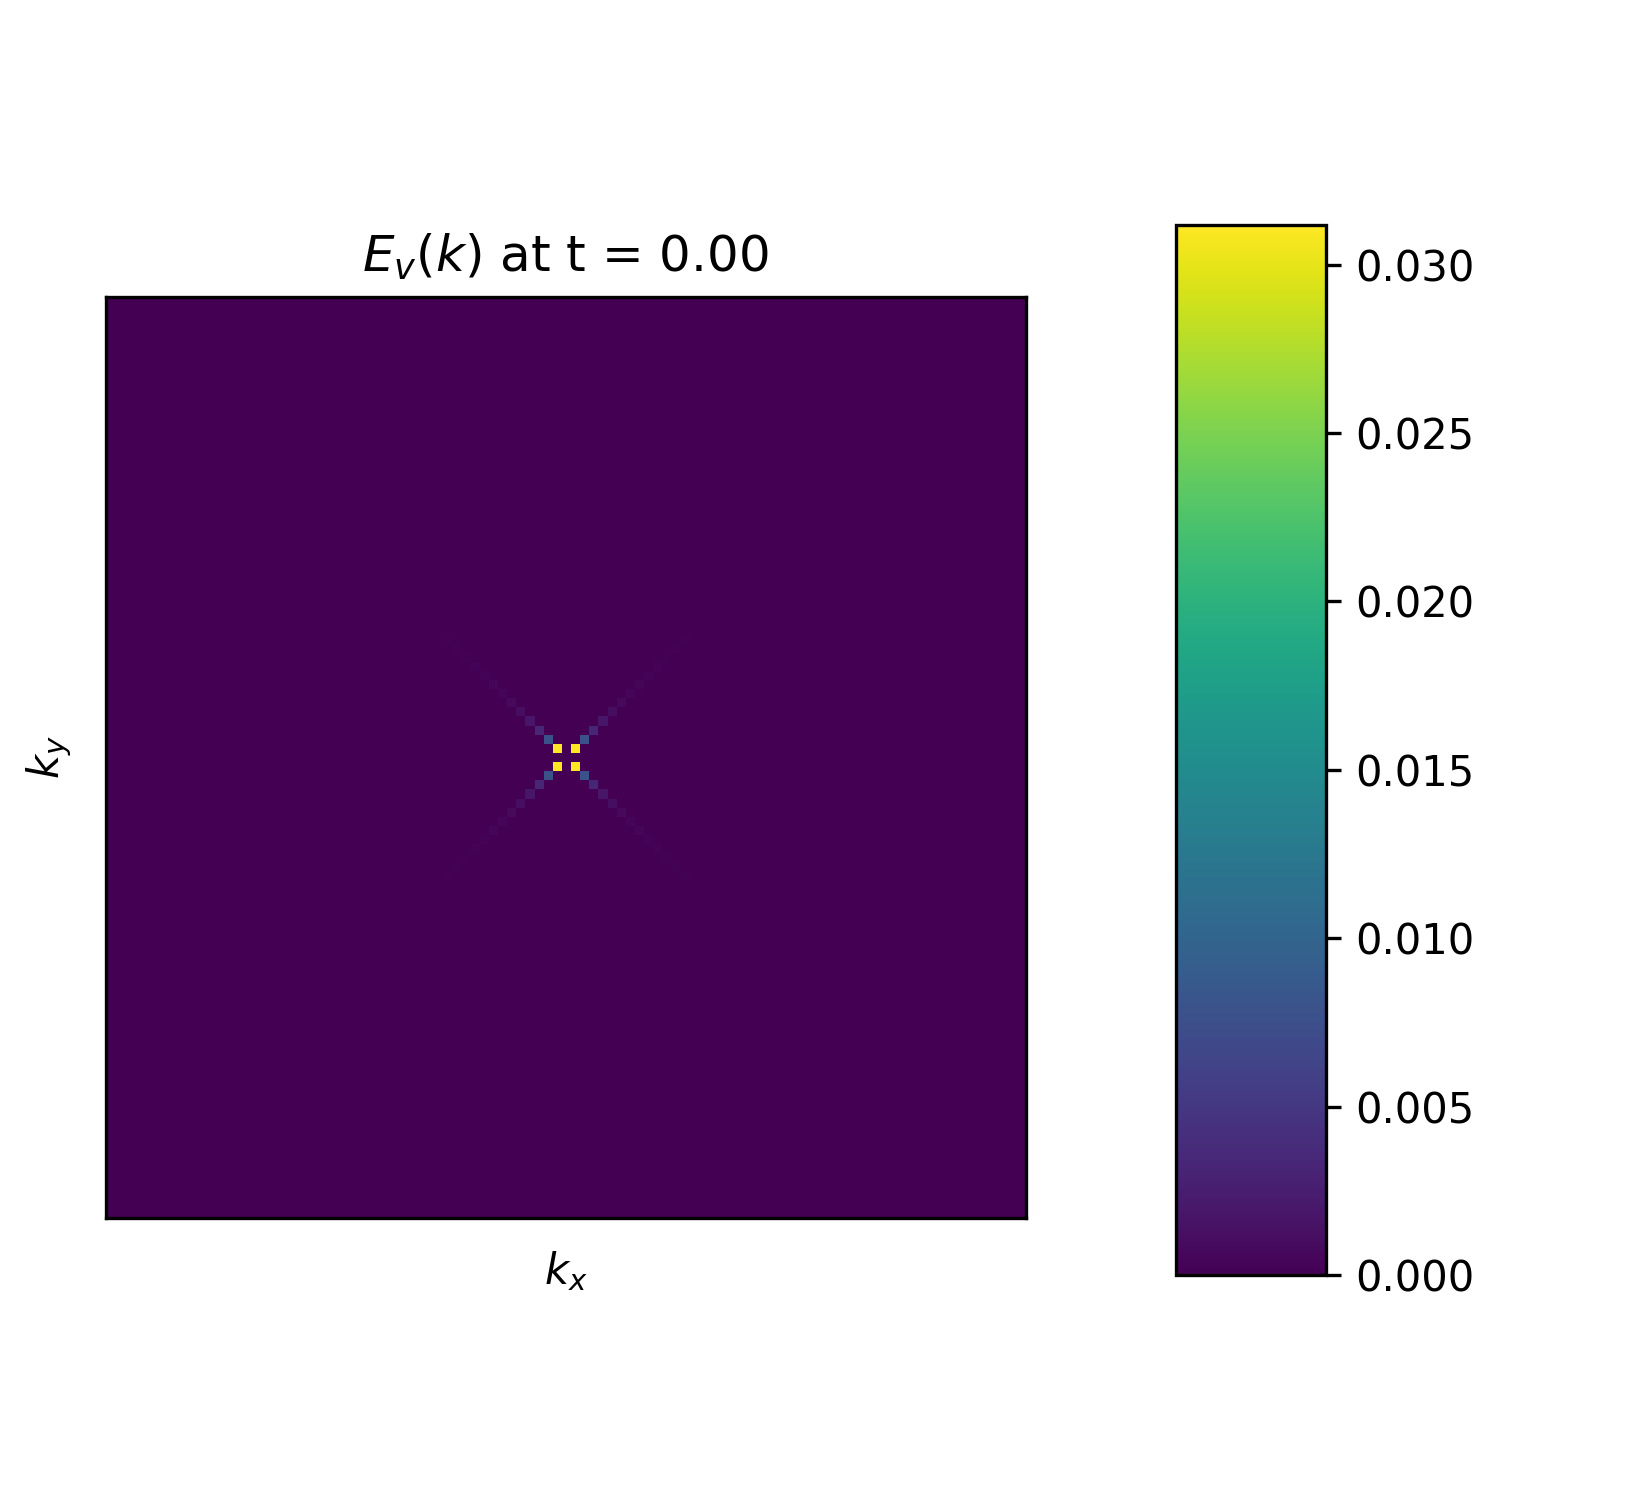
\includegraphics[width=6cm]{Code-Figures/sine-vel-prof-2d/EK_spectrum.png}
      \caption{$2D$ $\vect{E}(\vect{k})$ field}
    \end{subfigure}
    \caption{The vector fields $\vect{E}(\vect{k})$ for $1D$ and $2D$ case, with decay rate $\gamma=1$, and $N=n_x/2$.}
    \label{fig:espec-vector-fields-gamma1}
\end{figure}

\begin{figure}[H]
    \begin{subfigure}{7cm}
      \centering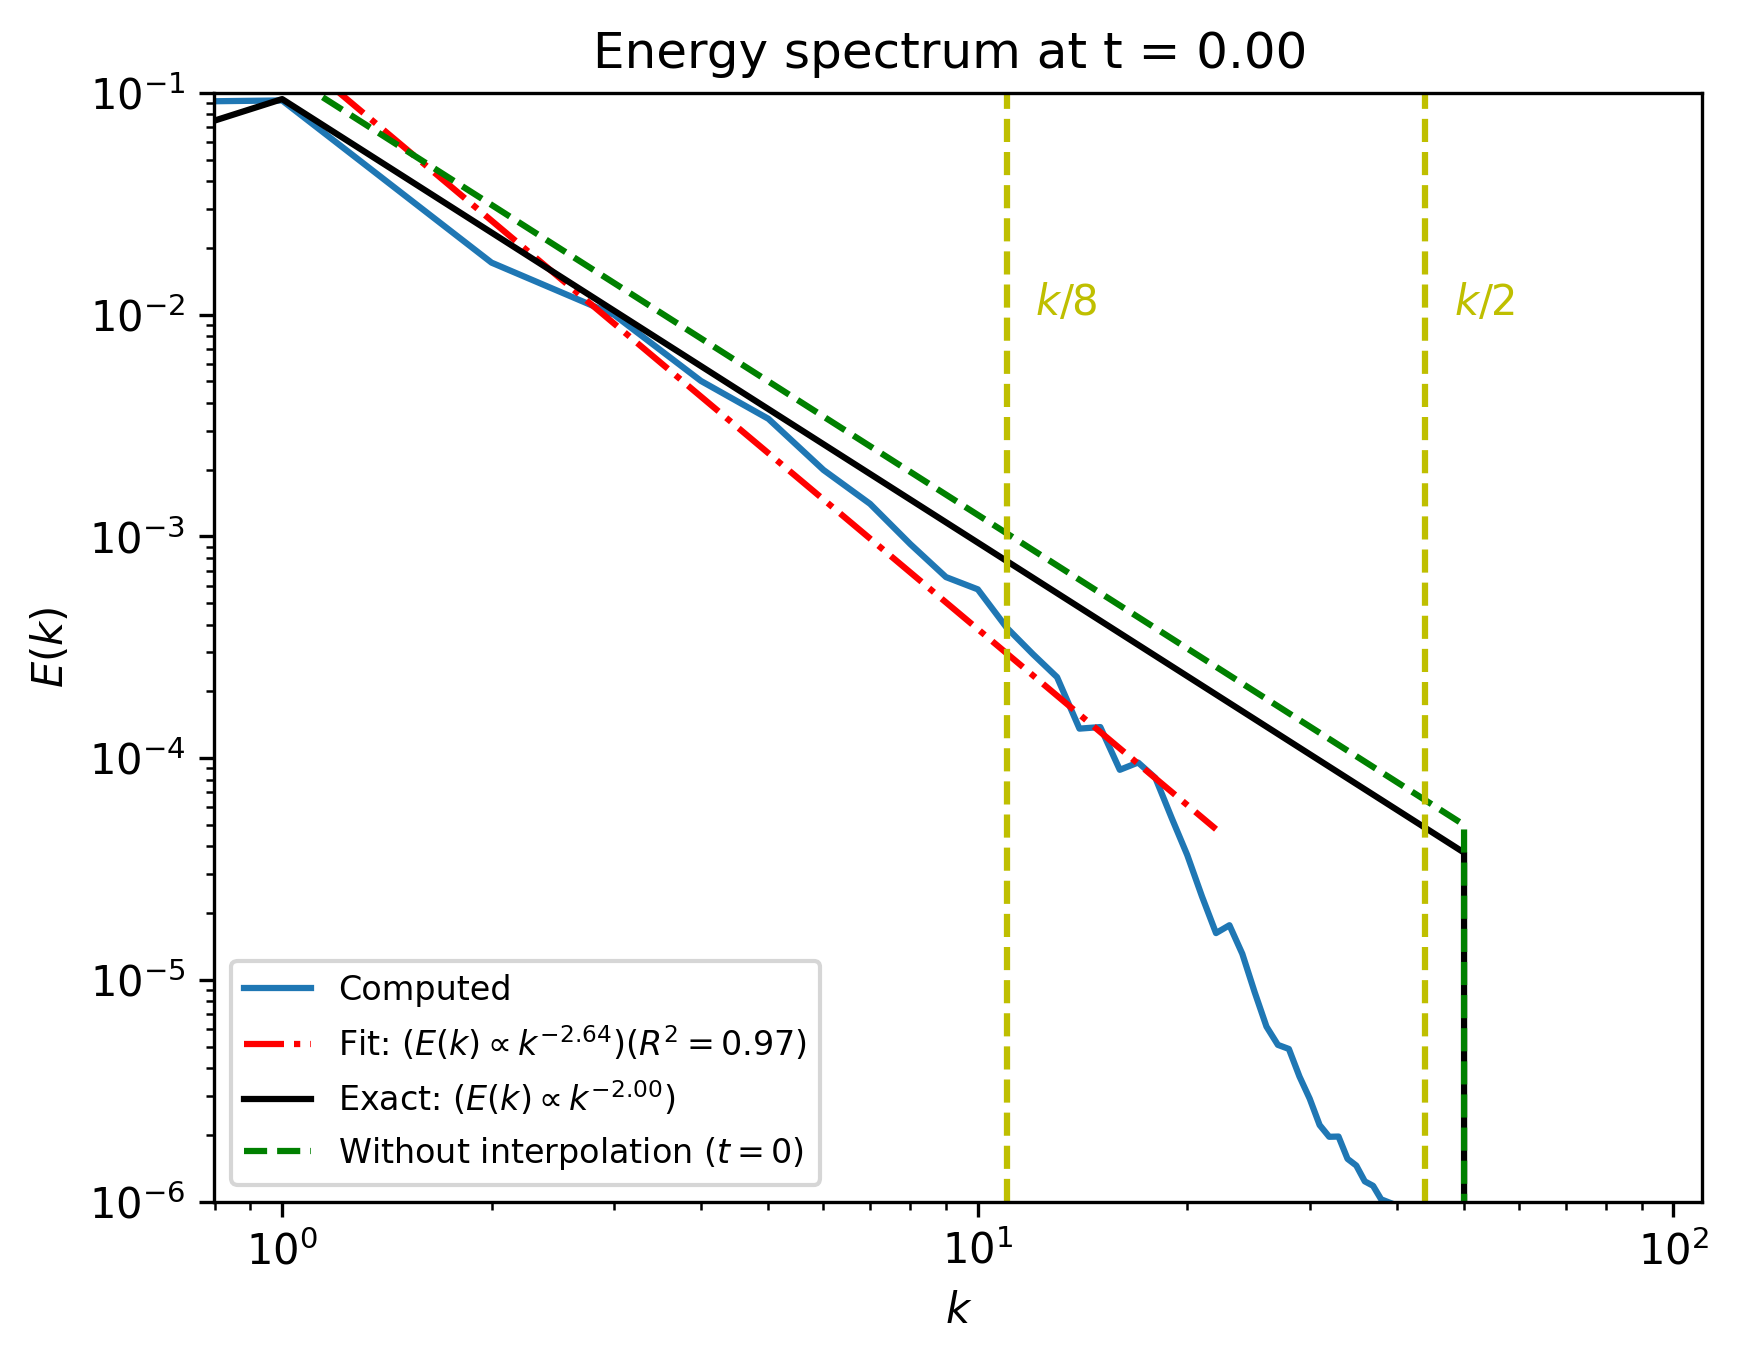
\includegraphics[width=6cm]{Code-Figures/sine-vel-prof-1d/ek_00000_loglog.png}
      \caption{$1D$ $E(k)$ field}
    \end{subfigure}
    \begin{subfigure}{7cm}
      \centering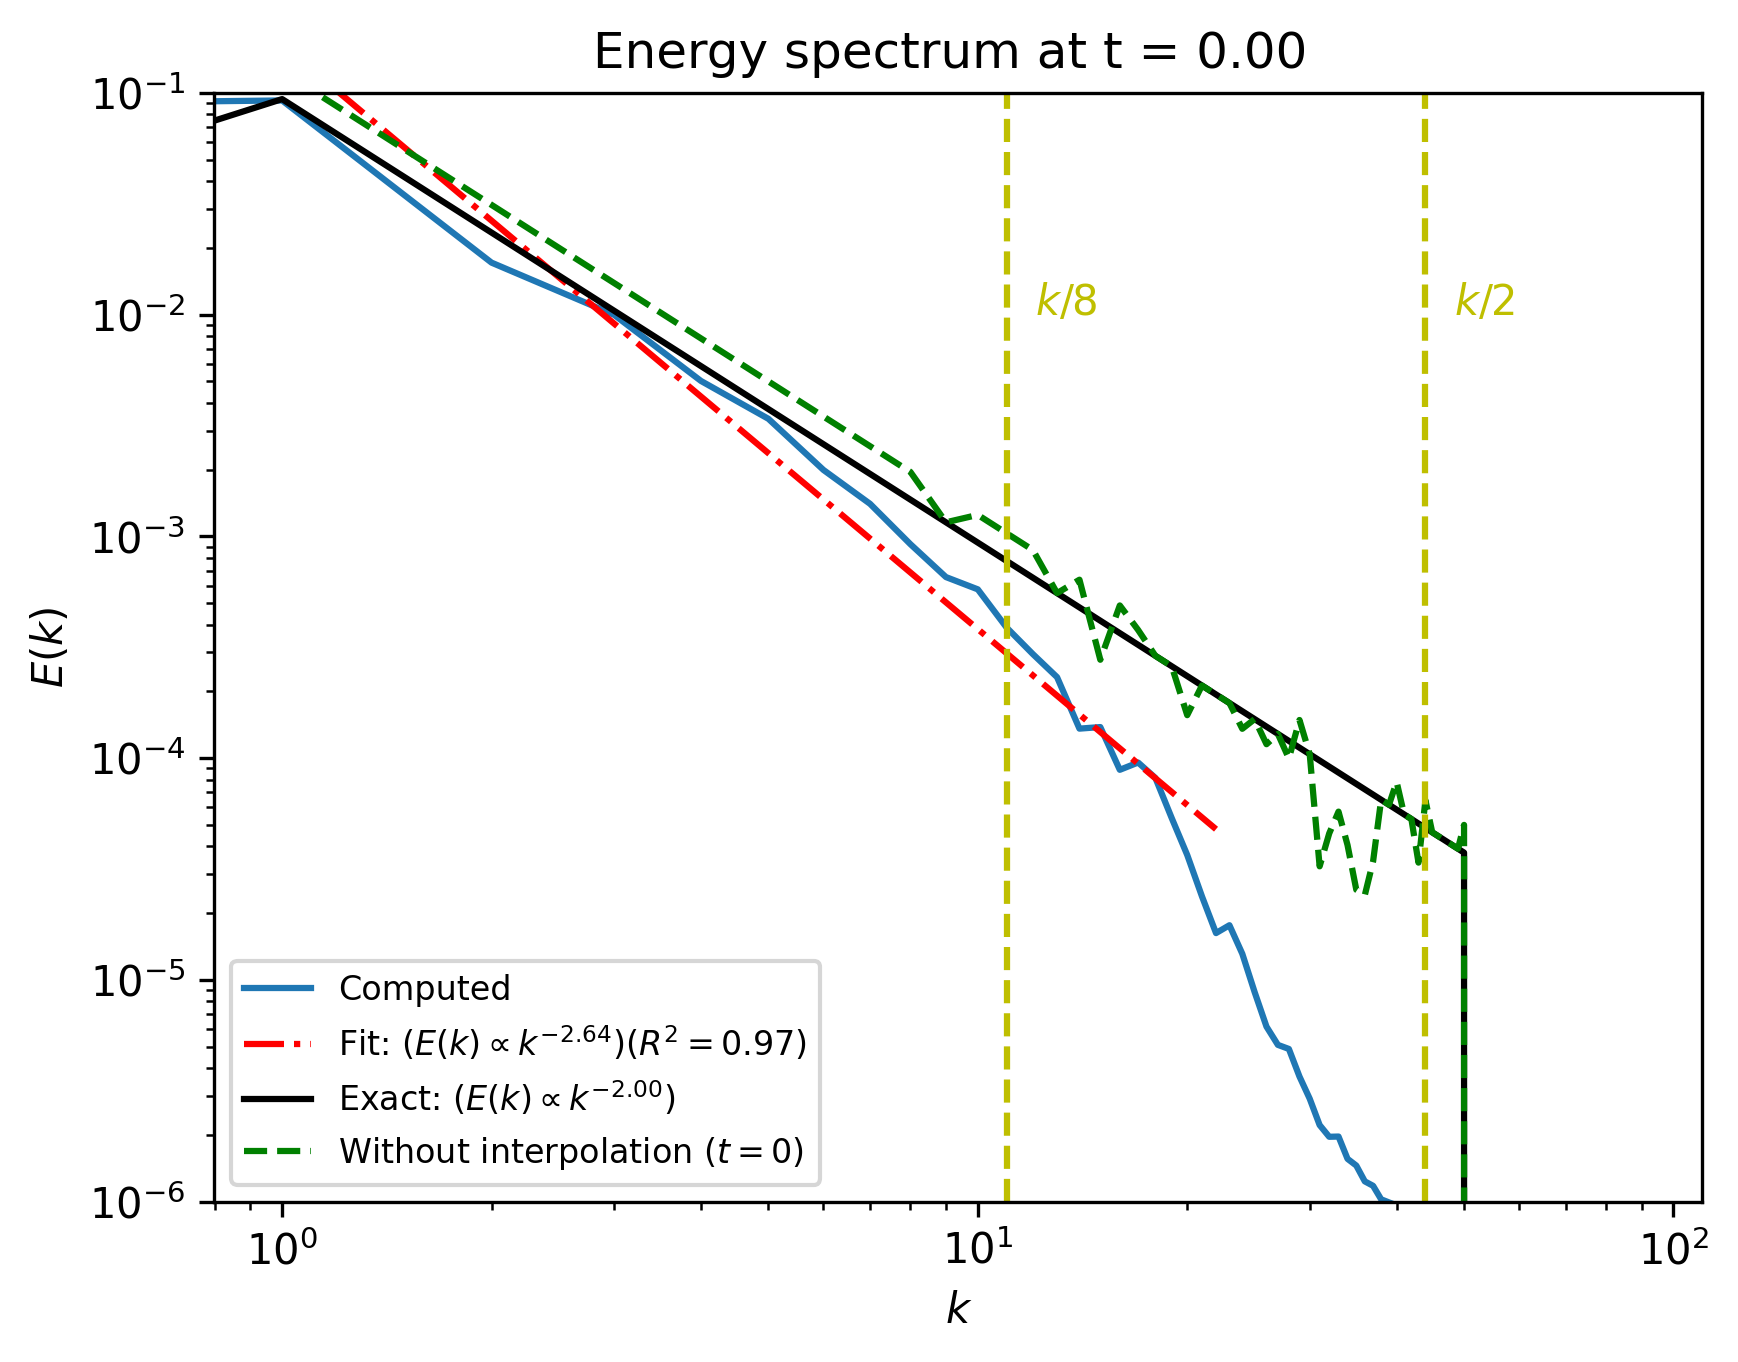
\includegraphics[width=6cm]{Code-Figures/sine-vel-prof-2d/ek_00000_loglog.png}
      \caption{$2D$ $E(k)$ field}
    \end{subfigure}
    \begin{subfigure}{7cm}
        \centering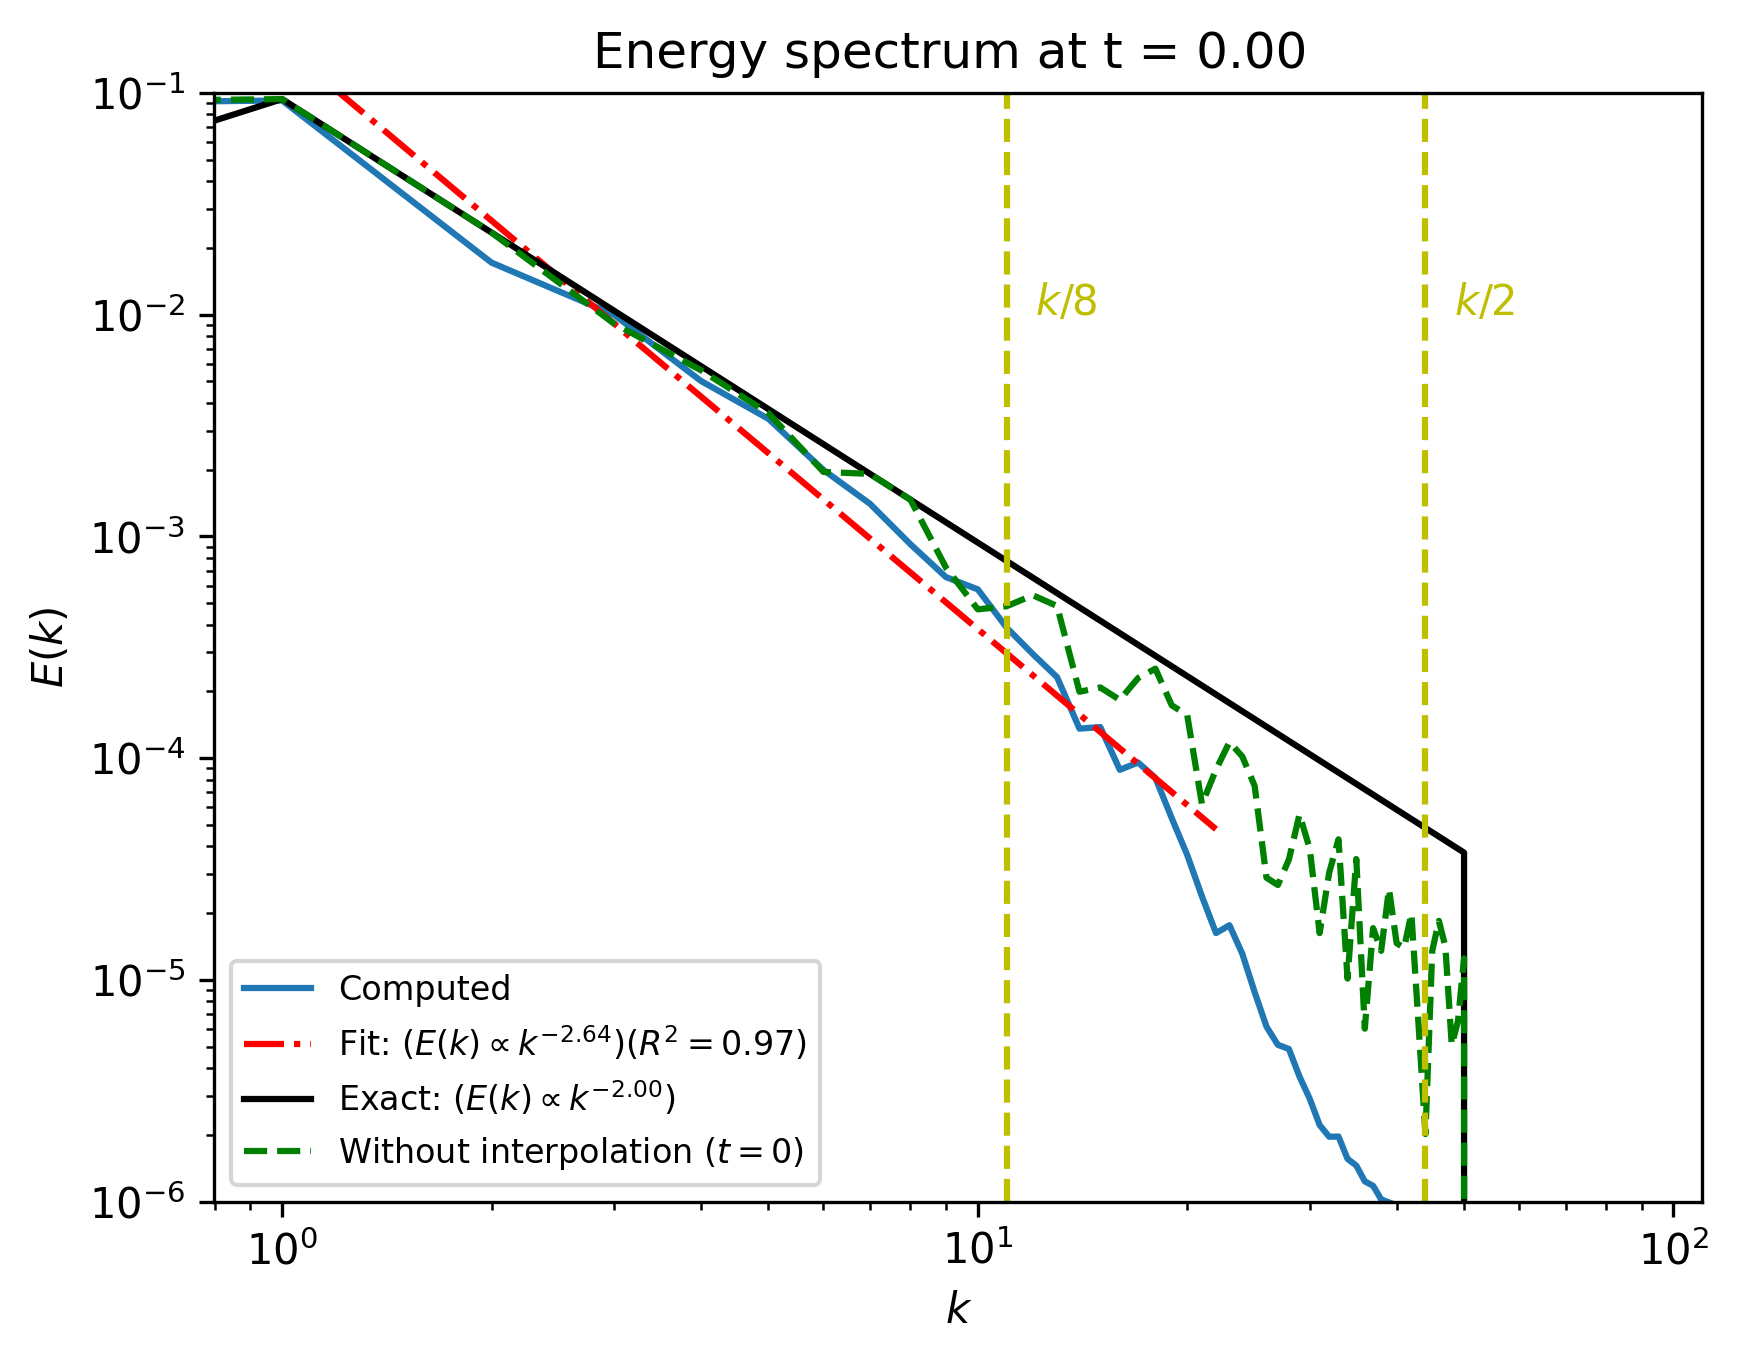
\includegraphics[width=6cm]{Code-Figures/sine-vel-prof-3d/ek_00000_loglog.png}
        \caption{$3D$ $E(k)$ field}
      \end{subfigure}
    \caption{The scalar fields $E(k)$ for $1D$, $2D$, and $3D$ case, with decay rate $\gamma=1$, and $N=n_x/2$.}
    \label{fig:espec-scalar-fields-gamma1}
\end{figure}

The same set of test-cases, with $\gamma=1$ and $N=n_x/2$, are considered, in order to identify the effect of various interpolation schemes, kernels, perturbation, and resolutions on the computed energy spectrum.

In order to measure the effect of the perturbation in the particle spacing on the computed energy spectrum, once a rectangluar grid of uniform particles are defined, its coordinates are perturbed by a uniform random number $\delta \hat{x} \in [0, 1)$, scaled by a perturbation amplitude. The perturbed grid is then initialised with the corresponding velocity profile, and the energy spectrum is computed for the perturbed grid. From the results shown in \figref{fig:espec-scalar-fields-per-ampl}, it can be observed that by increasing the perturbation amplitude, energy seems to be introduced at lower resolution scales, which is reflected by the icreased energy at higher wavenumbers. This trend seems to hold true, for all dimensions.
Therefore, we can infer that the low-pass energy dissipation effect of the interpolation scheme, will to an extent be countered by the perturbation in the particle spacing (which is typically the case in a simulation since the particles become disturbed), which will introduce energy at lower resolution scales, and hence, the slope of the energy spectrum computed from the interpolated velocity field, will be closer to the slope of the energy spectrum computed from the original velocity field. 

\begin{figure}[H]
    \begin{subfigure}{7cm}
      \centering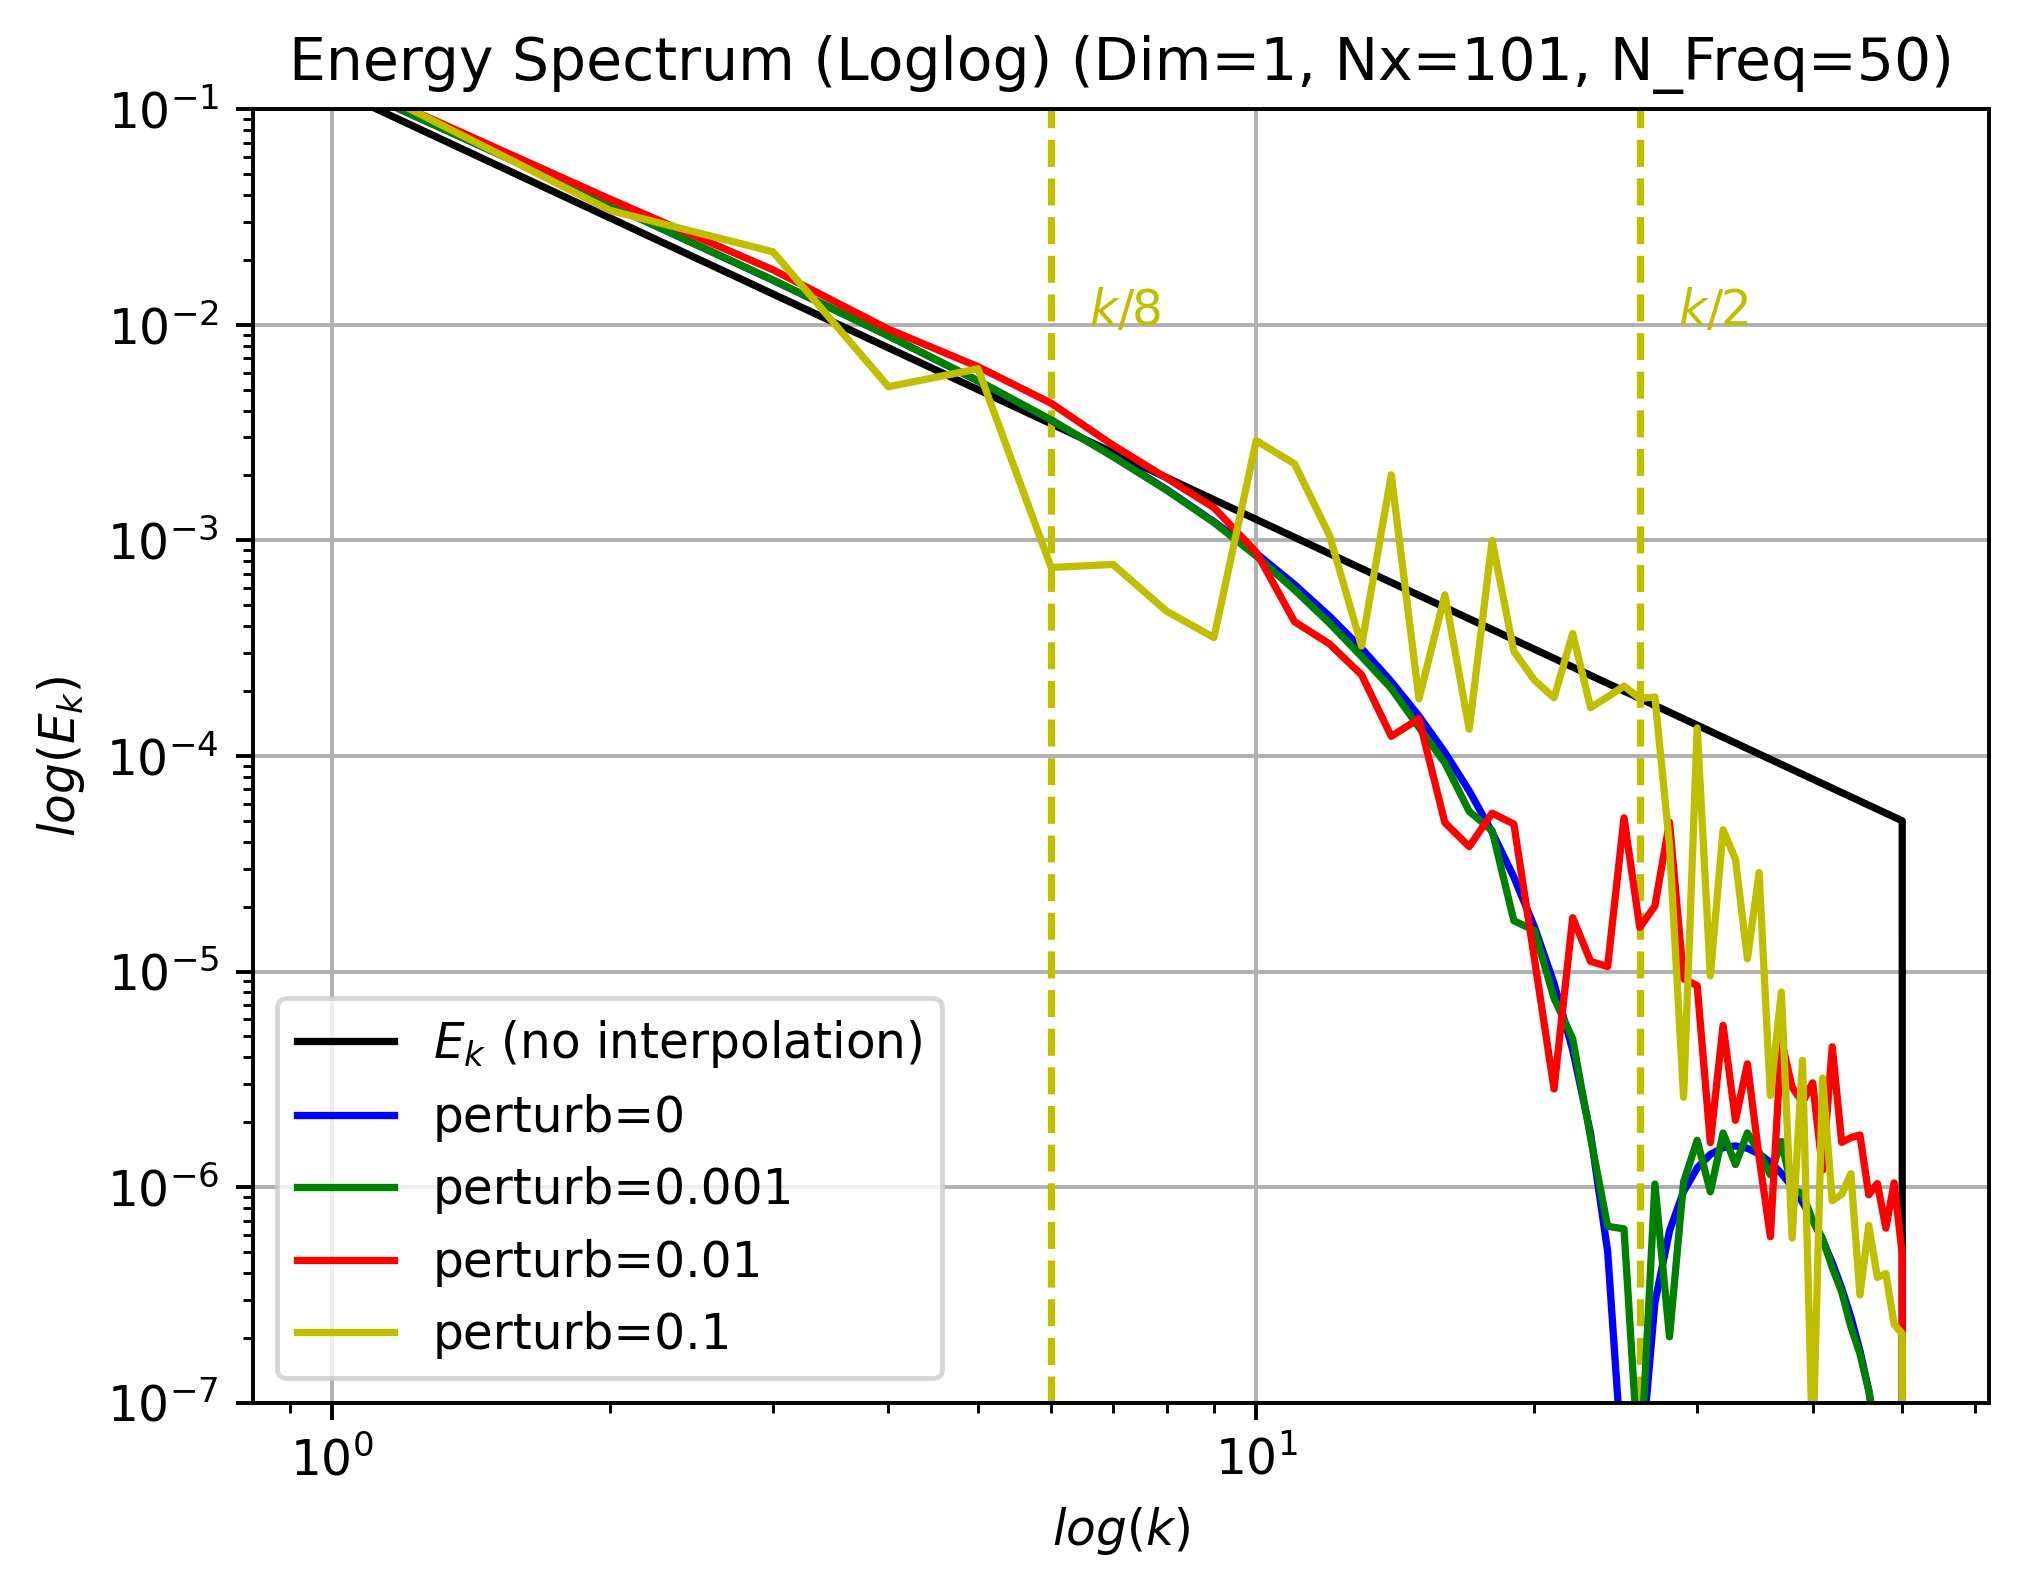
\includegraphics[width=6cm]{Code-Figures/sin-vel-prof-pertub/Energy Spectrum (Loglog) (Dim=1, Nx=101, N_Freq=50).png}
      \caption{$1D$ $E(k)$ field}
    \end{subfigure}
    \begin{subfigure}{7cm}
      \centering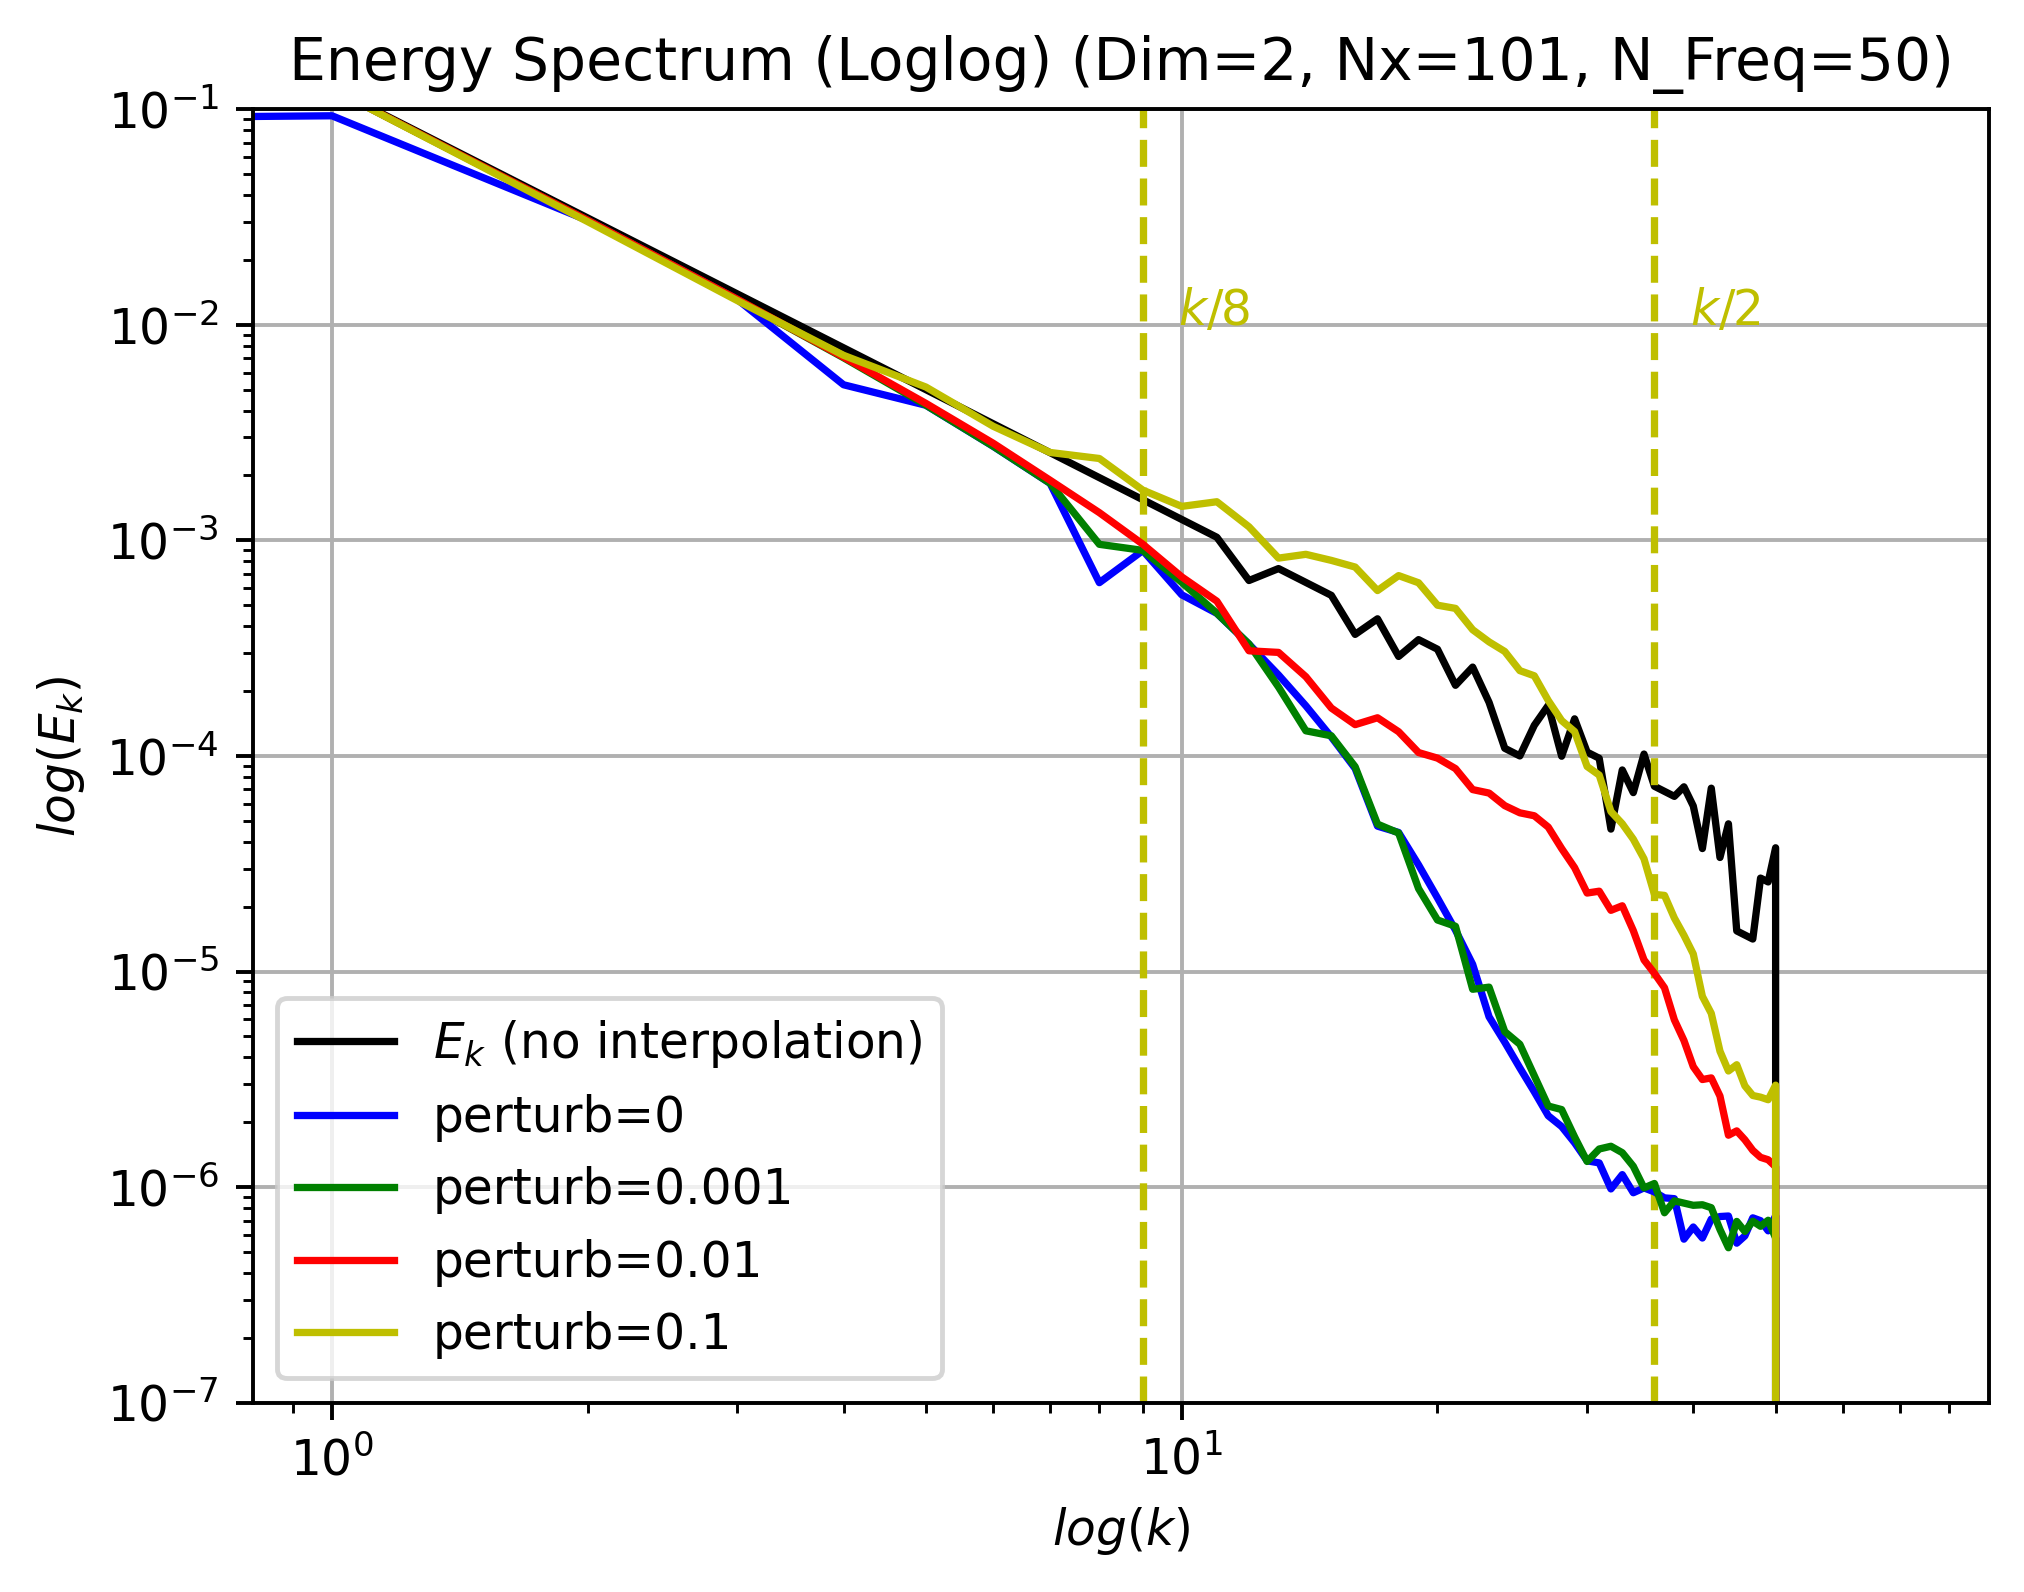
\includegraphics[width=6cm]{Code-Figures/sin-vel-prof-pertub/Energy Spectrum (Loglog) (Dim=2, Nx=101, N_Freq=50).png}
      \caption{$2D$ $E(k)$ field}
    \end{subfigure}
    \begin{subfigure}{7cm}
        \centering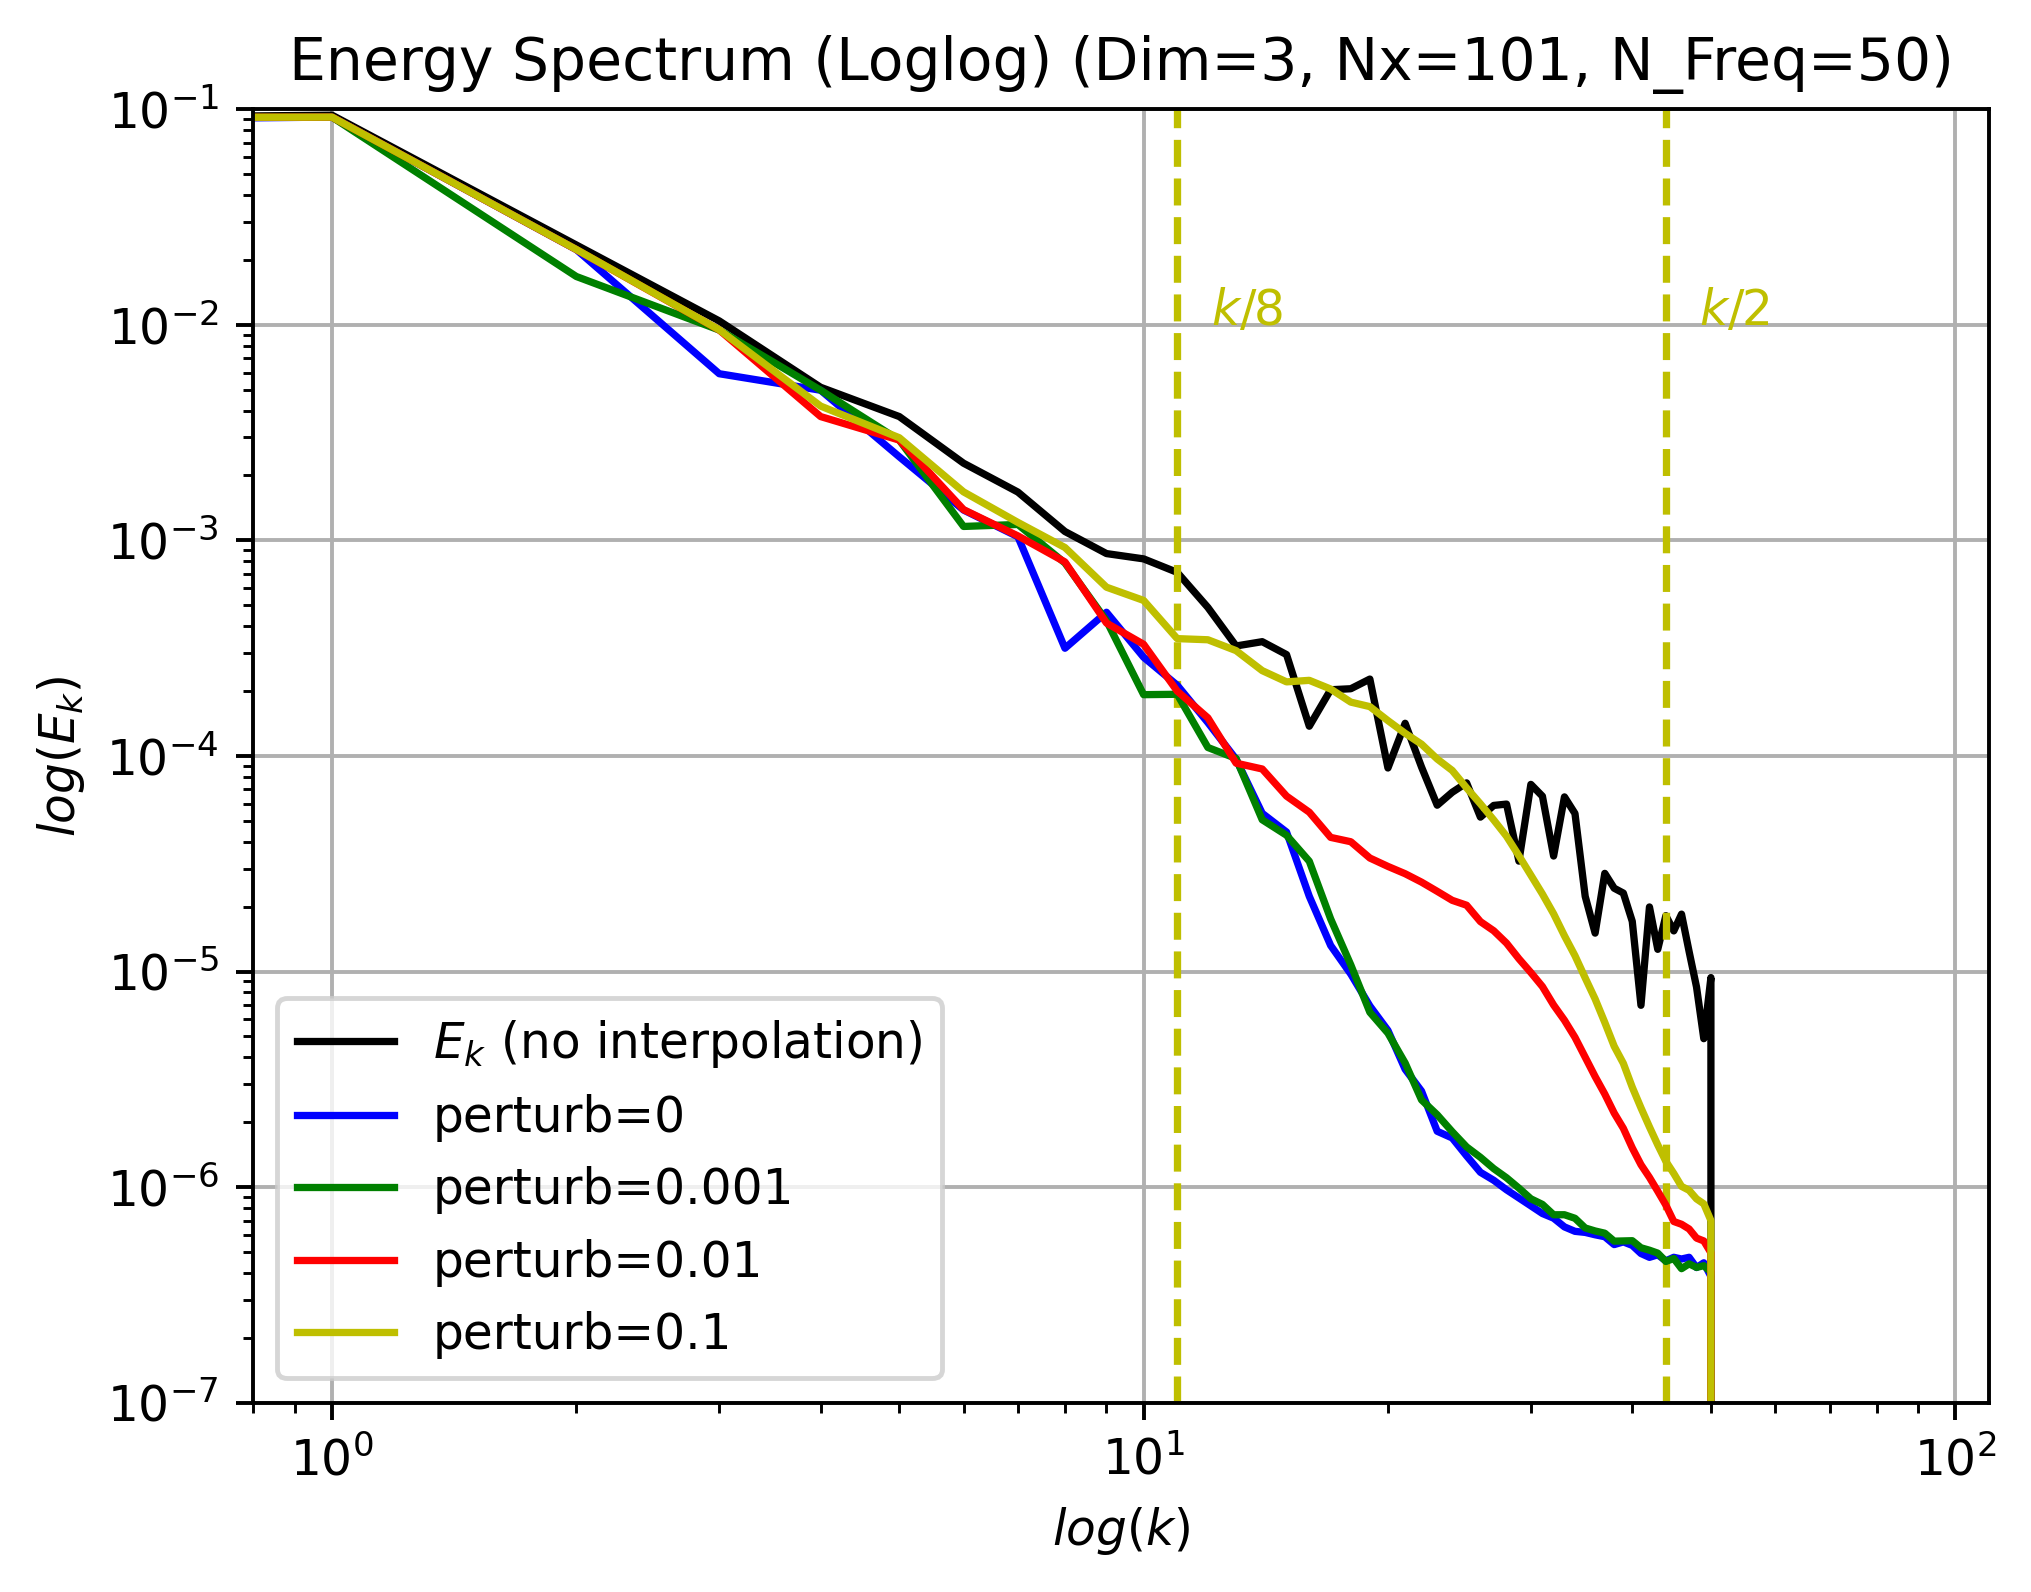
\includegraphics[width=6cm]{Code-Figures/sin-vel-prof-pertub/Energy Spectrum (Loglog) (Dim=3, Nx=101, N_Freq=50).png}
        \caption{$3D$ $E(k)$ field}
      \end{subfigure}
    \caption{The scalar fields $E(k)$ for $1D$, $2D$, and $3D$ case, for various perturbation amplitudes.}
    \label{fig:espec-scalar-fields-per-ampl}
\end{figure}

Then, in order to measure the effect of the interpolation scheme on the computed energy spectrum, the following interpolation schemes were considered:
\begin{itemize}
    \item \texttt{sph}:
    \begin{equation}
        \hat{\phi_i} = \sum_{ij} \frac{m_j}{\rho_j} \phi_j \DWIJ,
    \end{equation}
    
    \item \texttt{shepard}:
    \begin{equation}
        \hat{\phi_i} = \frac{\sum_{ij} \phi_j \WIJ}{\sum_{ij} \WIJ},
    \end{equation}

    \item \texttt{order1} \parencite{Liu2006}:
    \begin{equation}
      \tensor{A}_{4 \times 4} \vect{x}_{4 \times 1} = \vect{b}_{4 \times 1}
      \label{eq:interp-order1}
    \end{equation}
    where, $\tensor{A}$ is the moment matrix, $\vect{b} = [\phi, \nabla \phi]^T$ is the interpolated property and its gradient calculated using basic SPH, and $\vect{x} = [\hat{\phi}, \nabla \hat{\phi}]^T$ is the unknown interpolated property and its gradient,

    \item \texttt{order1BL}: same as \Eqref{eq:interp-order1}, but with the $\DWIJ$ term corrected using the Bonet-Lok correction \parencite{bonet1999variational},

    \item \texttt{order1MC}: same as \Eqref{eq:interp-order1}, but with the $\DWIJ$ term corrected using the Mixed-Kernel correction \parencite{bonet1999variational},
\end{itemize}
where $\phi$ is the quantity to be interpolated, and $\hat{\phi}$ is the interpolated quantity.

From the results shown in \figref{fig:espec-scalar-fields-i-methods}, it can be observed that the \texttt{order1MC} interpolation scheme, seems to introduce the least amount of energy at lower resolution scales, with the \texttt{sph} scheme introducing the most amount of energy at lower resolution scales. This trend seems to hold true, for all dimensions.
Therefore, considering the fact that the \texttt{sph} interpolation scheme would appear to counter the loss in energy at lower resolution scales, due to the act of interpolation, it is chosen as the default interpolation scheme for the computation of the energy spectrum.

\begin{figure}[H]
	\begin{subfigure}{7cm}
		\centering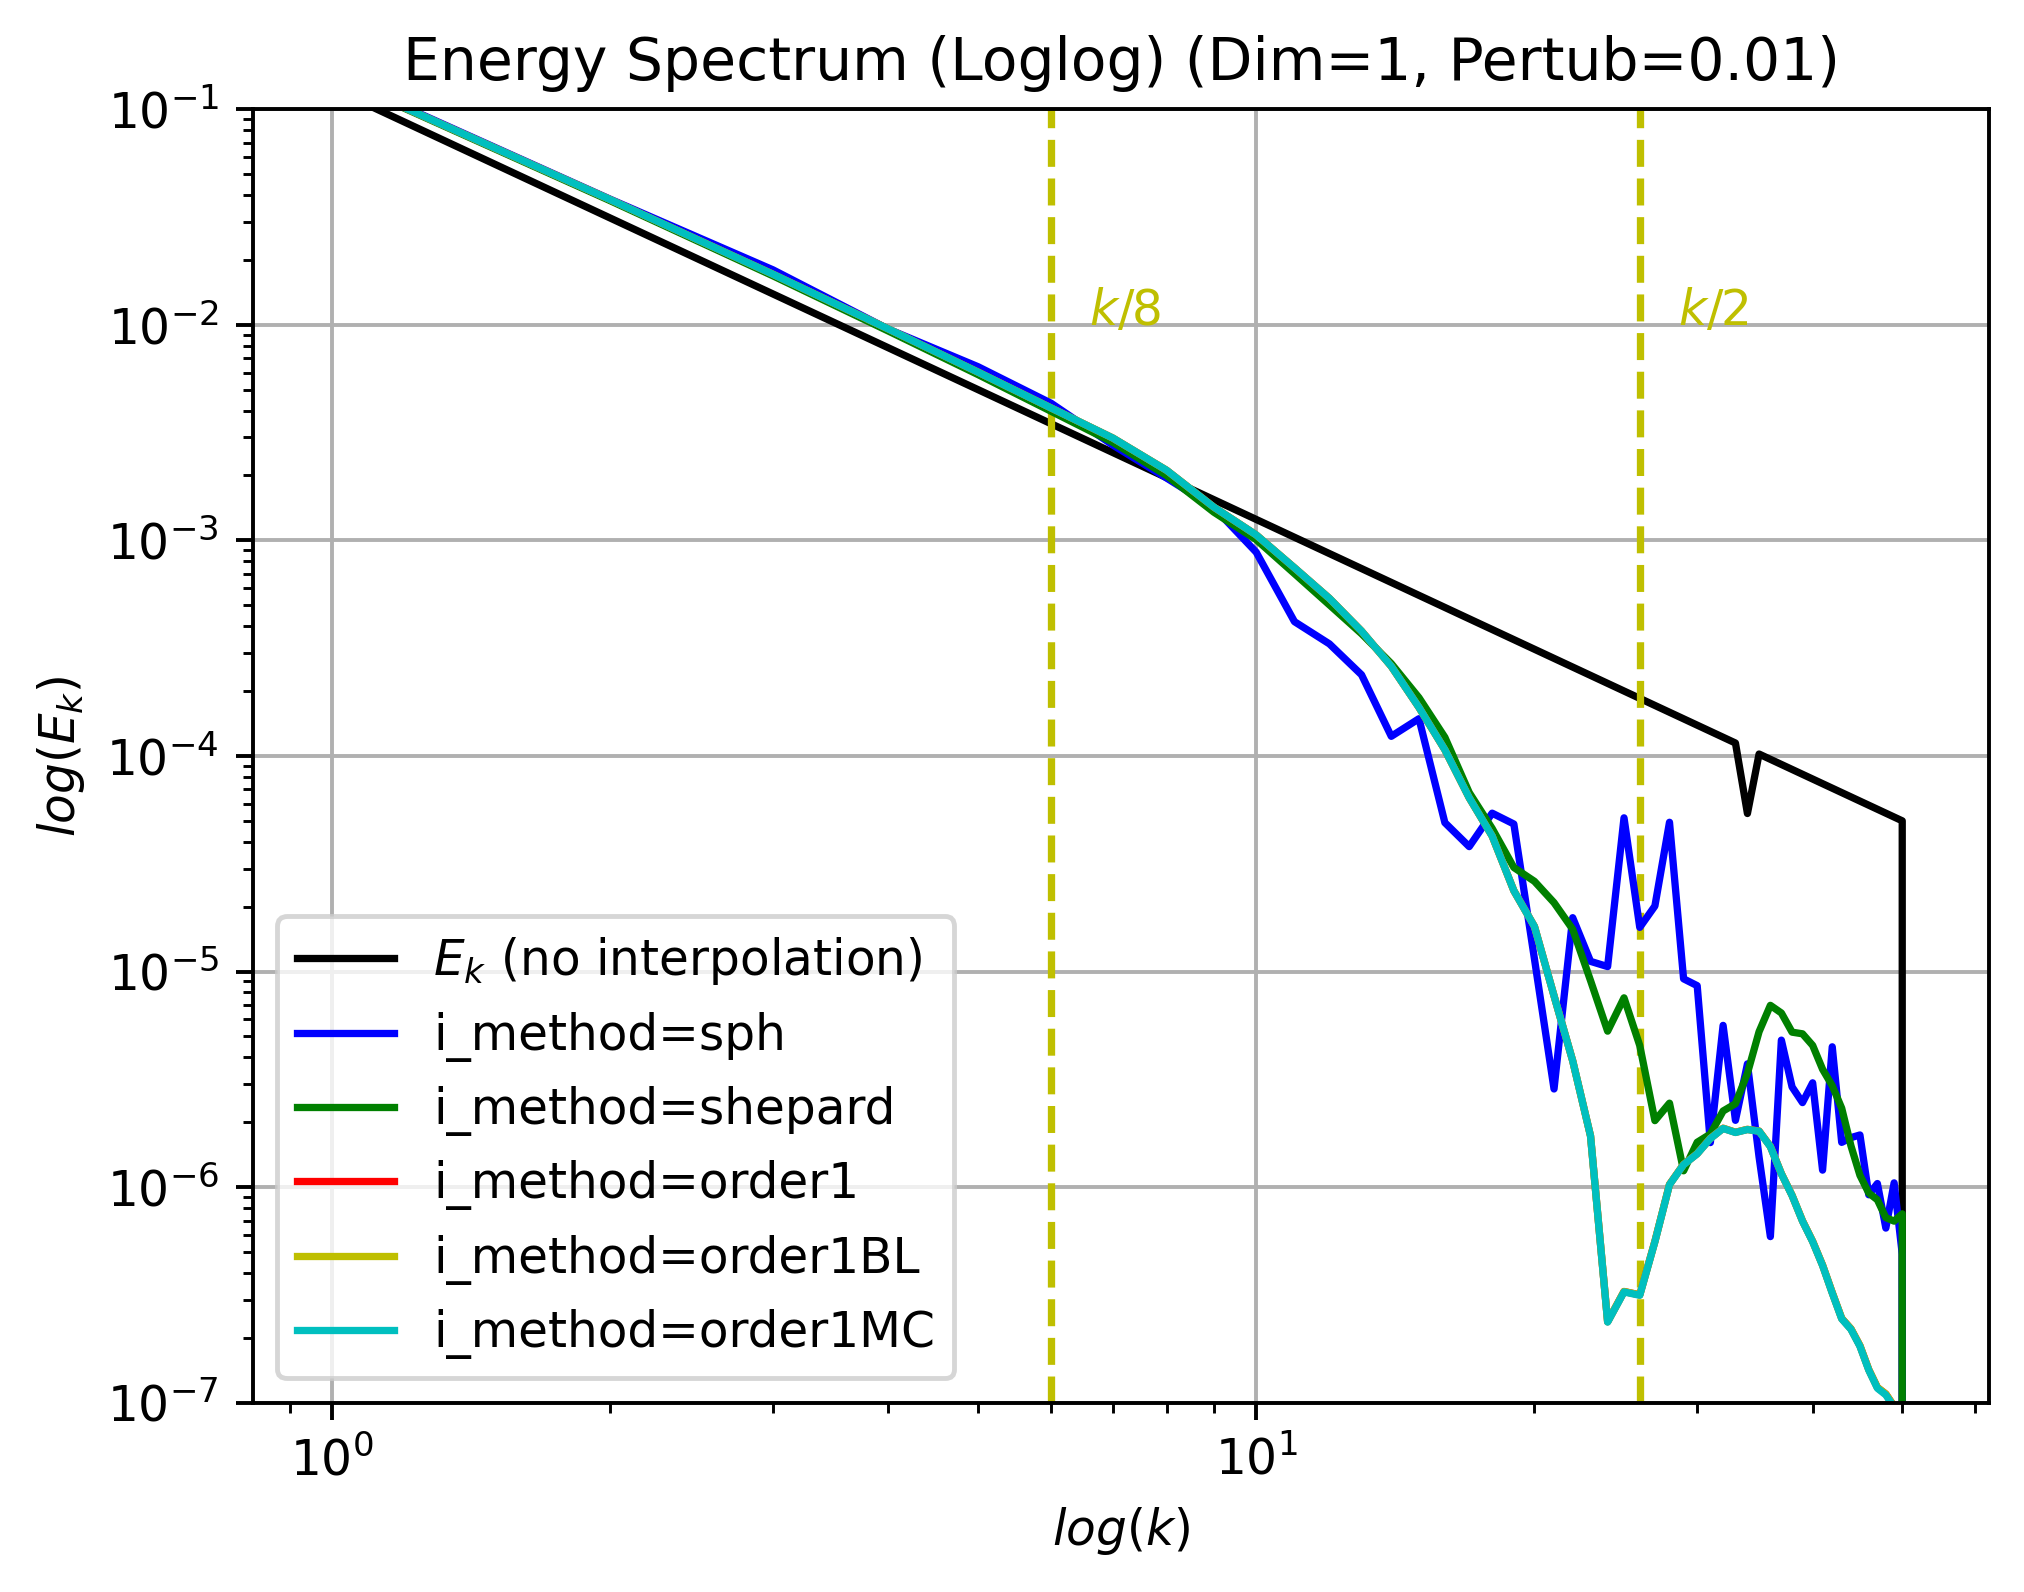
\includegraphics[width=6cm]{Code-Figures/sin-vel-prof-i-methods/Energy Spectrum (Loglog) (Dim=1, Pertub=0.01).png}
		\caption{$1D$ $E(k)$ field}
	\end{subfigure}
	\begin{subfigure}{7cm}
		\centering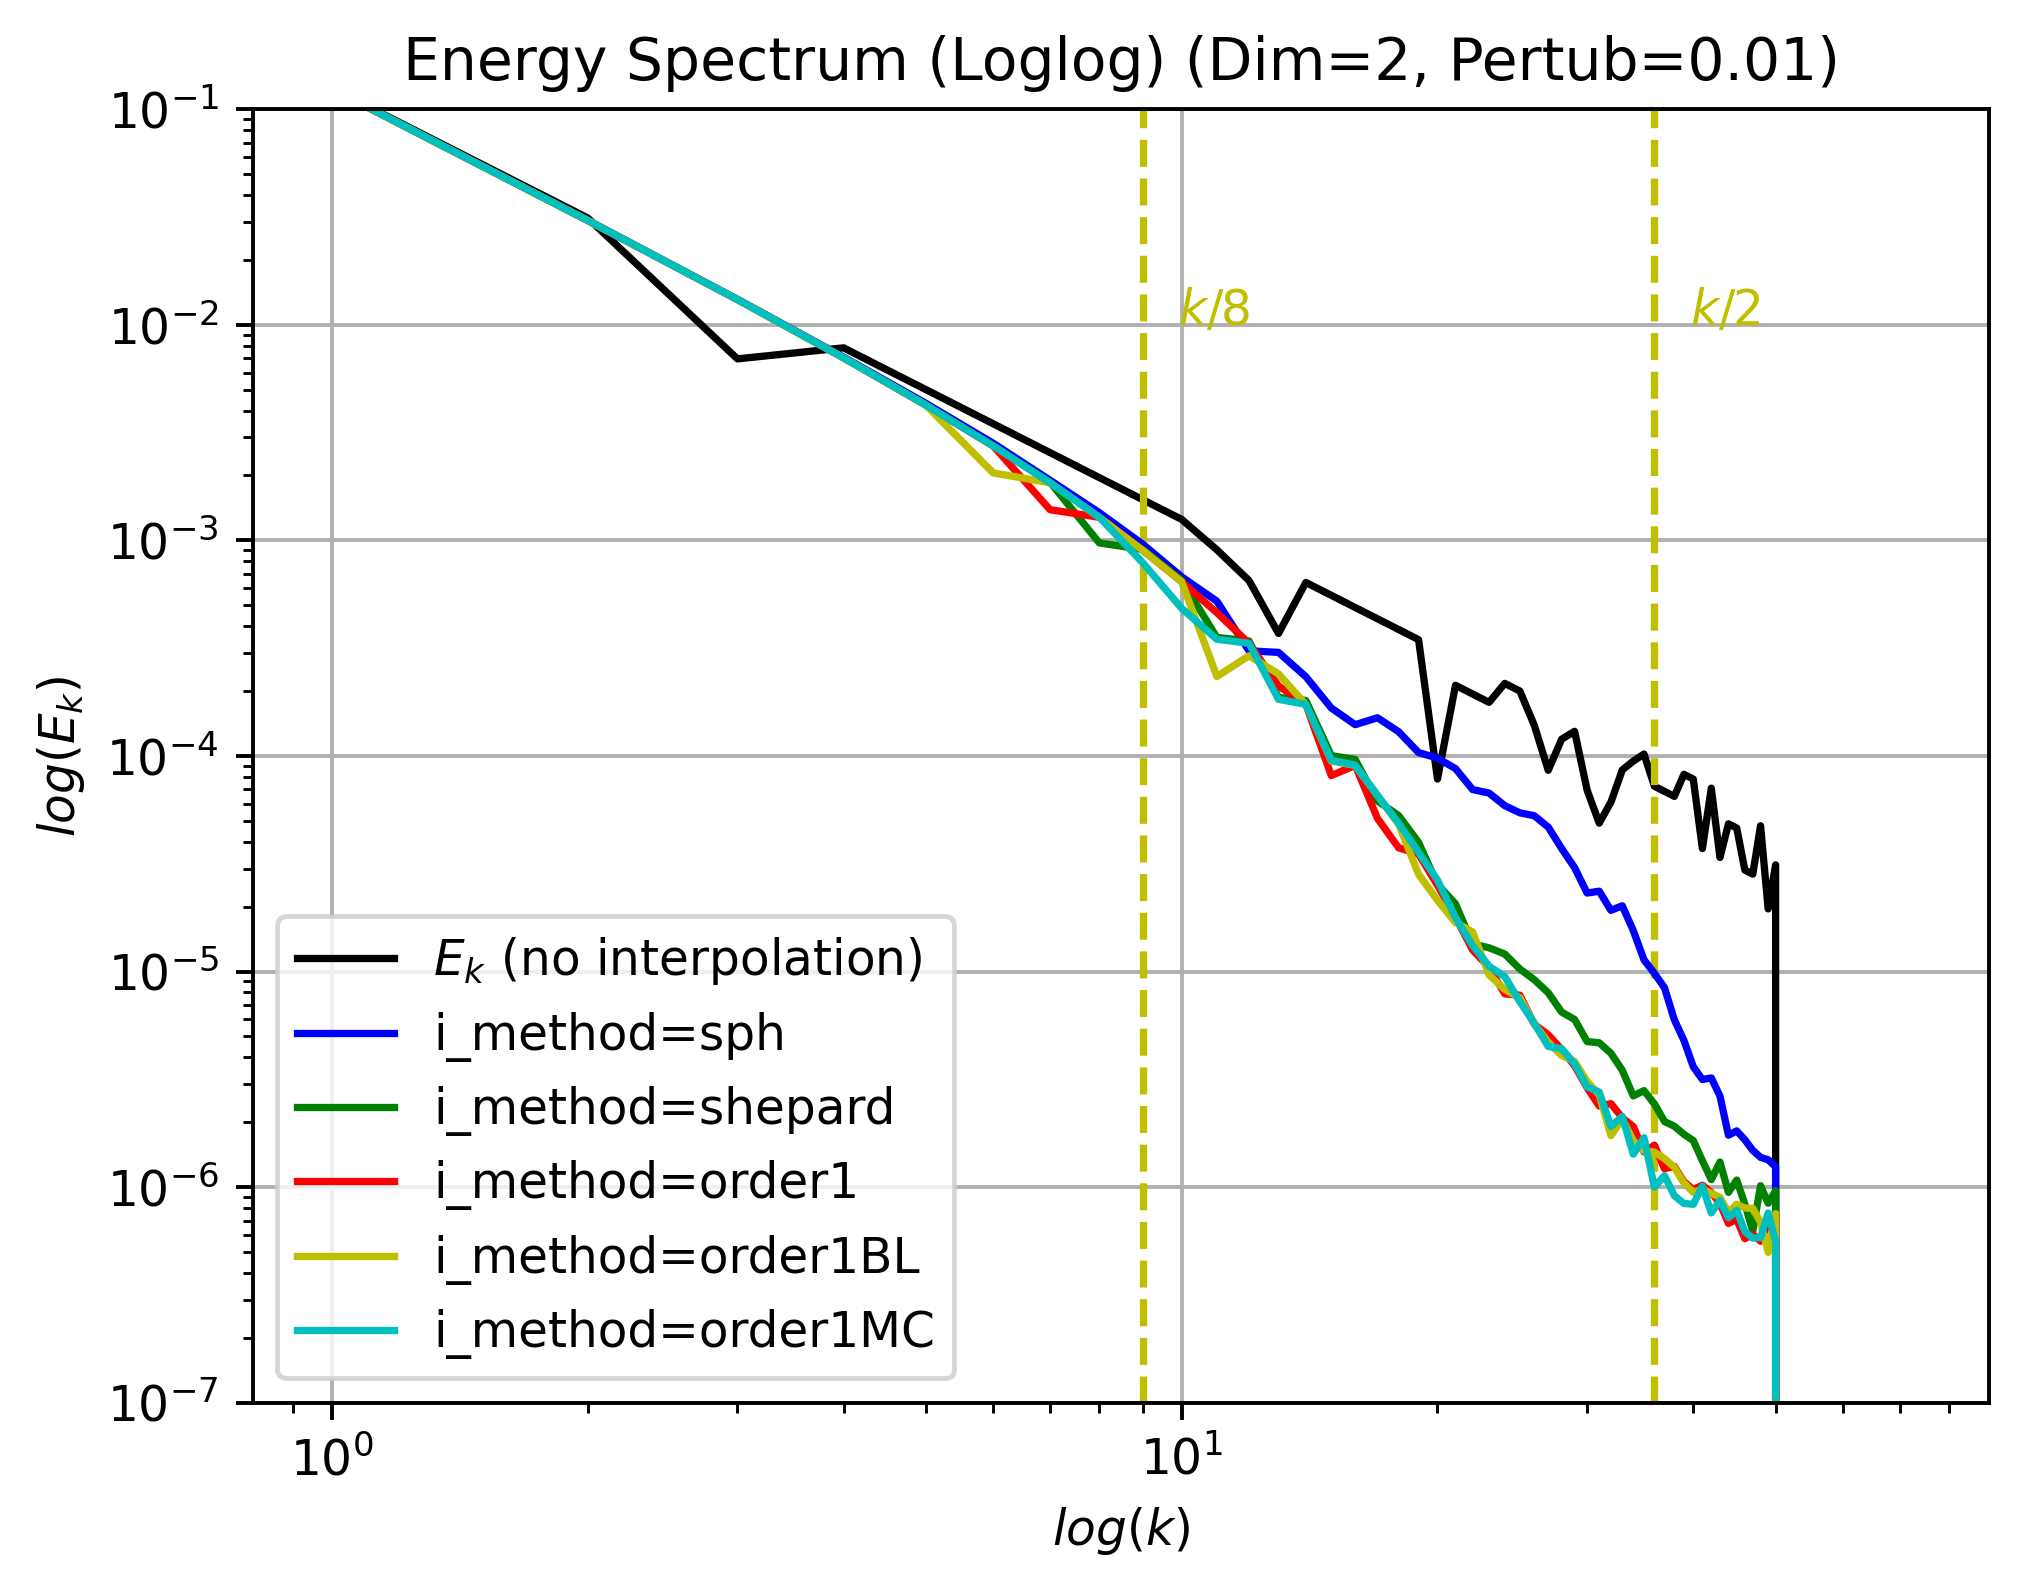
\includegraphics[width=6cm]{Code-Figures/sin-vel-prof-i-methods/Energy Spectrum (Loglog) (Dim=2, Pertub=0.01).png}
		\caption{$2D$ $E(k)$ field}
	\end{subfigure}
	\begin{subfigure}{7cm}
		\centering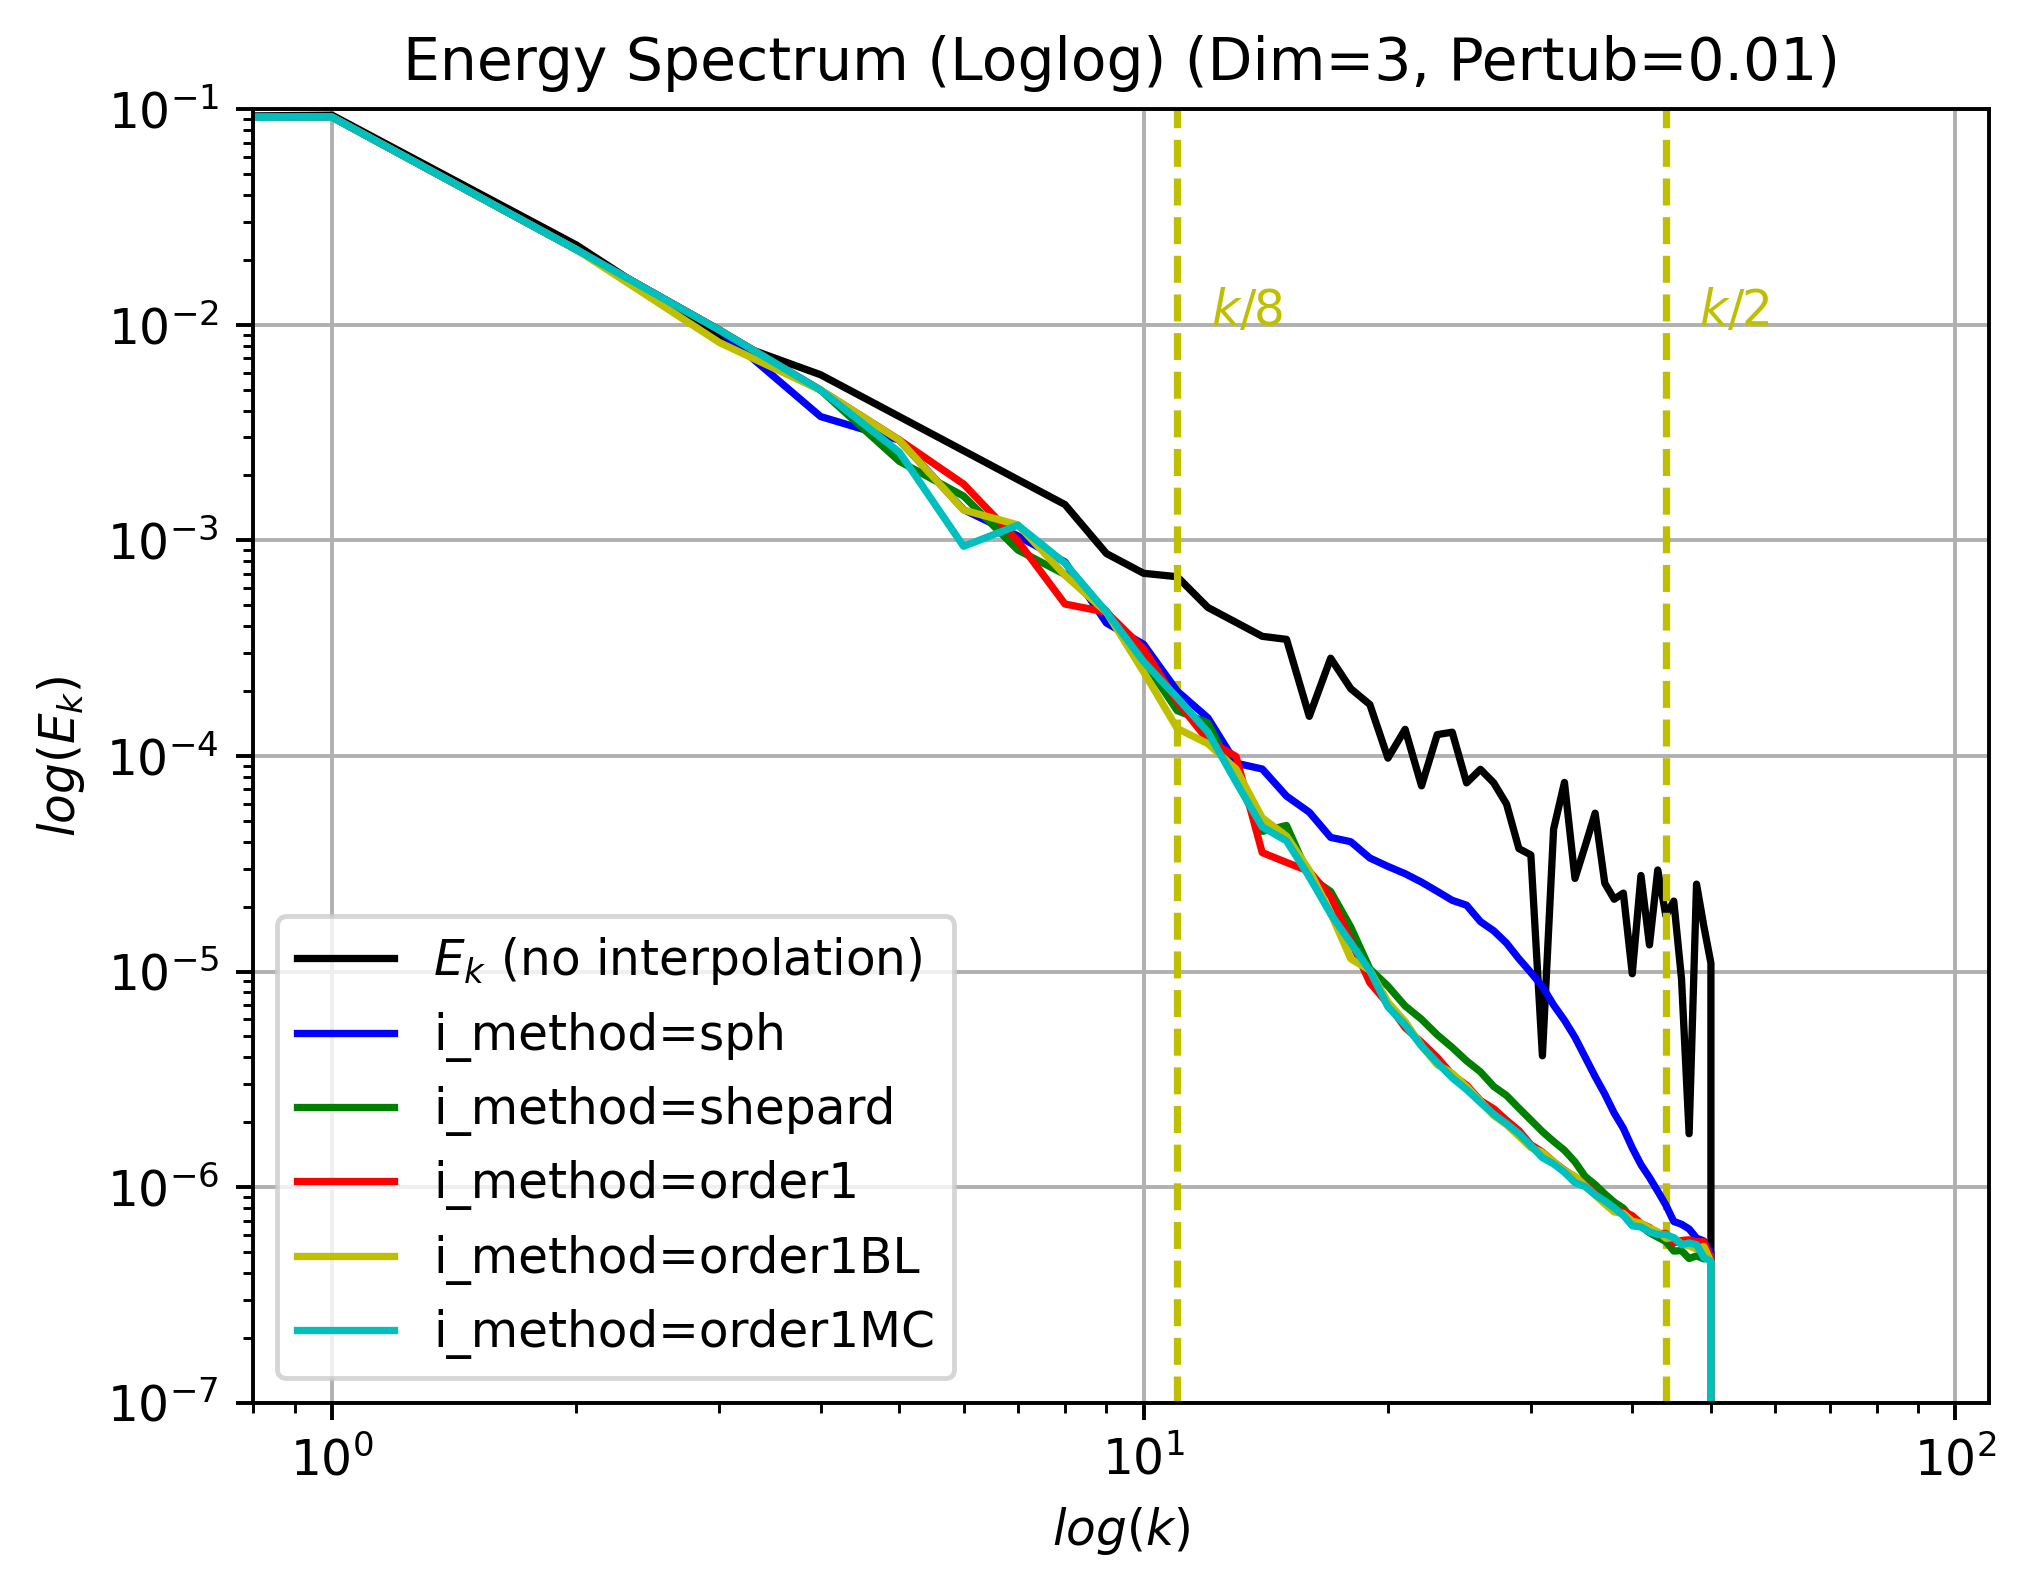
\includegraphics[width=6cm]{Code-Figures/sin-vel-prof-i-methods/Energy Spectrum (Loglog) (Dim=3, Pertub=0.01).png}
		\caption{$3D$ $E(k)$ field}
	\end{subfigure}
	\caption{The scalar fields $E(k)$ for $1D$, $2D$, and $3D$ case, for various interpolation schemes.}
	\label{fig:espec-scalar-fields-i-methods}
\end{figure}

Then, in order to measure the effect of the kernel on the computed energy spectrum, the following kernels were considered:
\begin{itemize}
    \item \texttt{CubicSpline},
    \item \texttt{WendlandQuinticC2},
    \item \texttt{WendlandQuinticC4},
    \item \texttt{WendlandQuinticC6},
    \item \texttt{Gaussian},
    \item \texttt{SuperGaussian},
    \item \texttt{QuinticSpline}.
\end{itemize}

From the results shown in \figref{fig:espec-scalar-fields-i-kernels}, it can be observed that the \texttt{Gaussian} kernel, seems to introduce the least amount of energy at lower resolution scales, with the \texttt{WendlandQuinticC6} kernel introducing the most amount of energy at lower resolution scales. This trend seems to hold true, for all dimensions.
Therefore, the \texttt{Gaussian} kernel is chosen as the default kernel for the computation of the energy spectrum.

\begin{figure}[H]
	\begin{subfigure}{7cm}
		\centering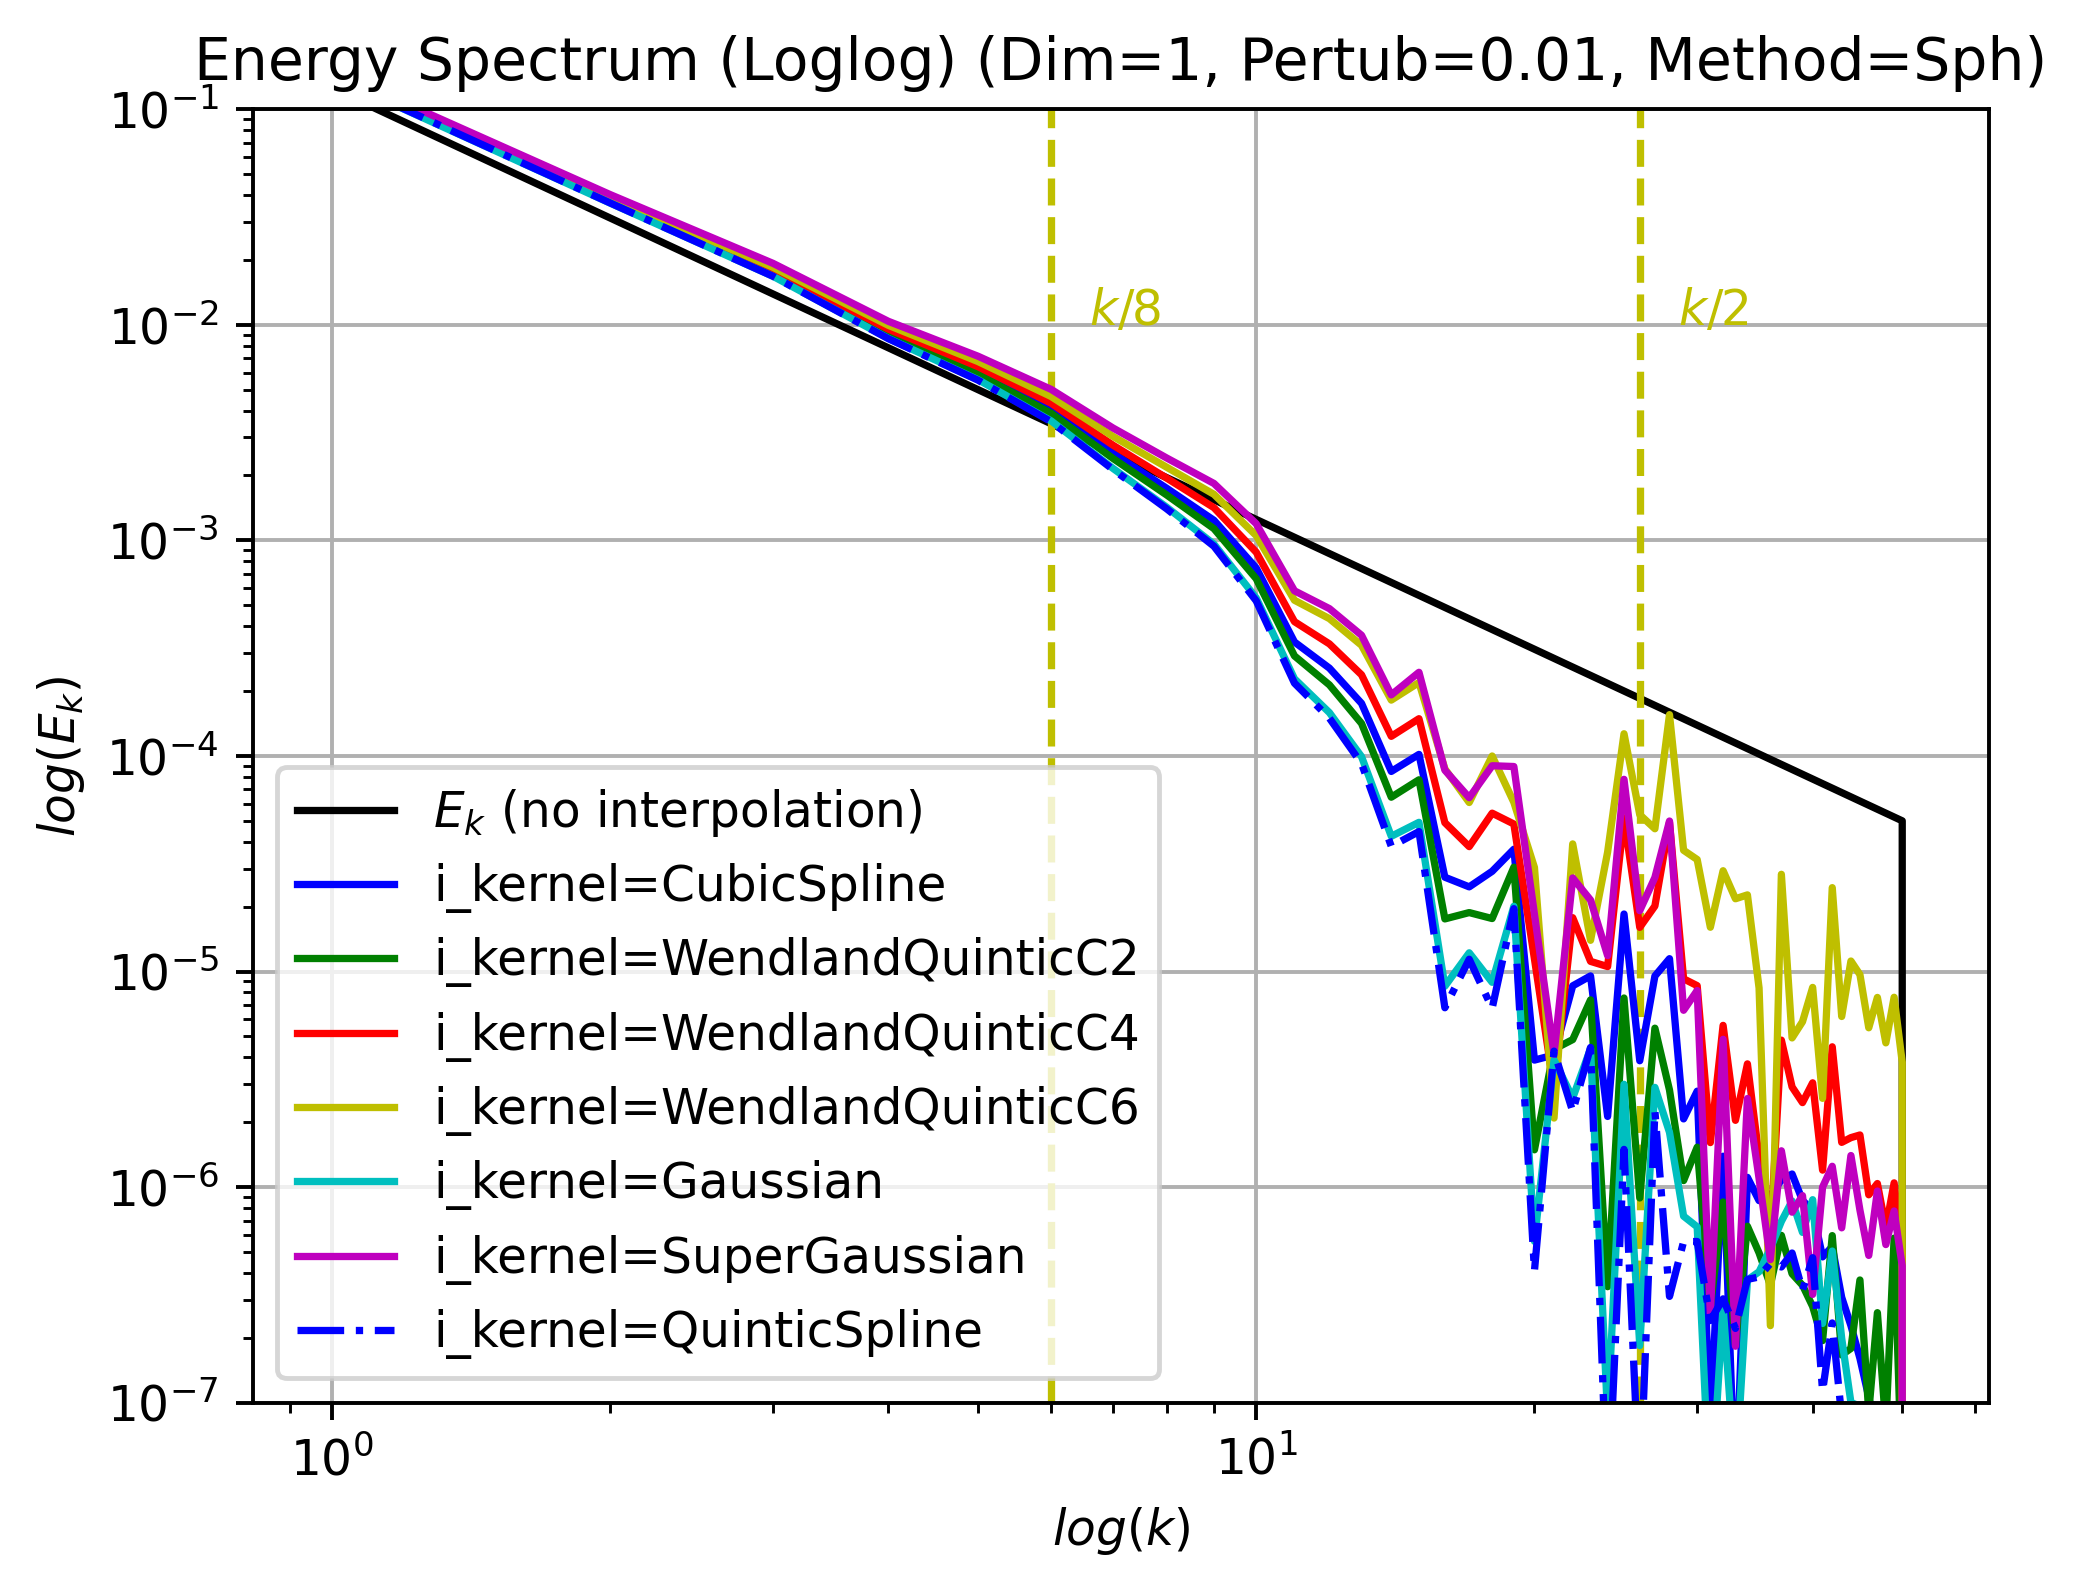
\includegraphics[width=6cm]{Code-Figures/sin-vel-prof-i-kernel/Energy Spectrum (Loglog) (Dim=1, Pertub=0.01, Method=Sph).png}
		\caption{$1D$ $E(k)$ field}
	\end{subfigure}
	\begin{subfigure}{7cm}
		\centering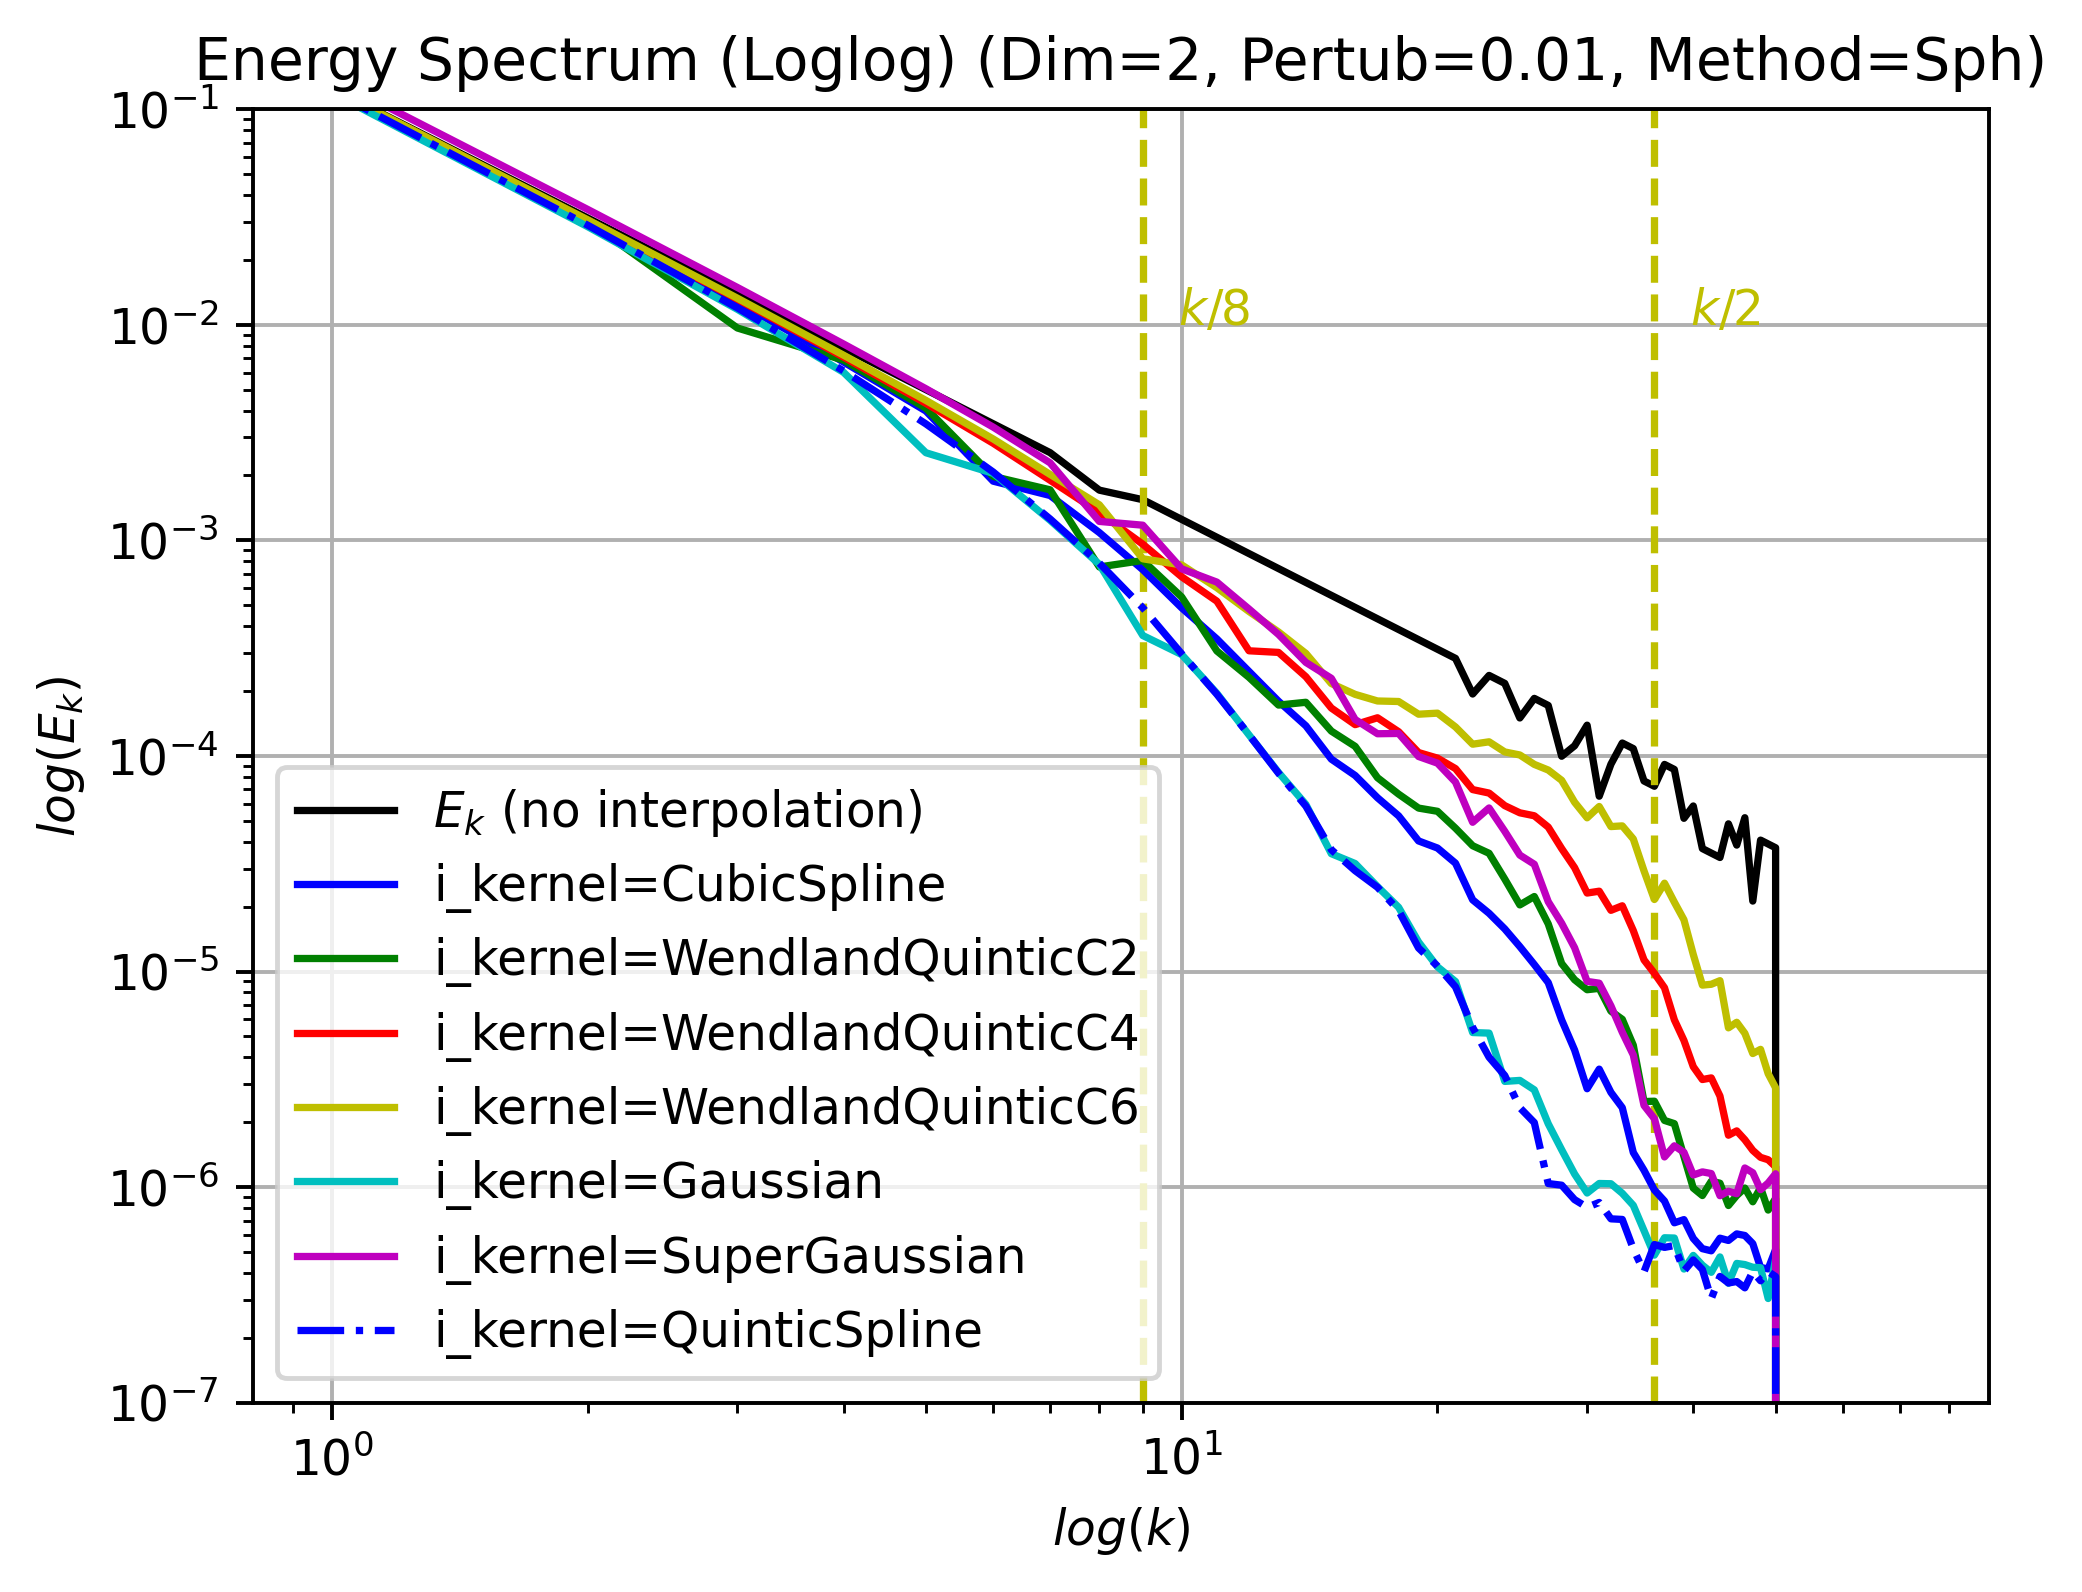
\includegraphics[width=6cm]{Code-Figures/sin-vel-prof-i-kernel/Energy Spectrum (Loglog) (Dim=2, Pertub=0.01, Method=Sph).png}
		\caption{$2D$ $E(k)$ field}
	\end{subfigure}
	\begin{subfigure}{7cm}
		\centering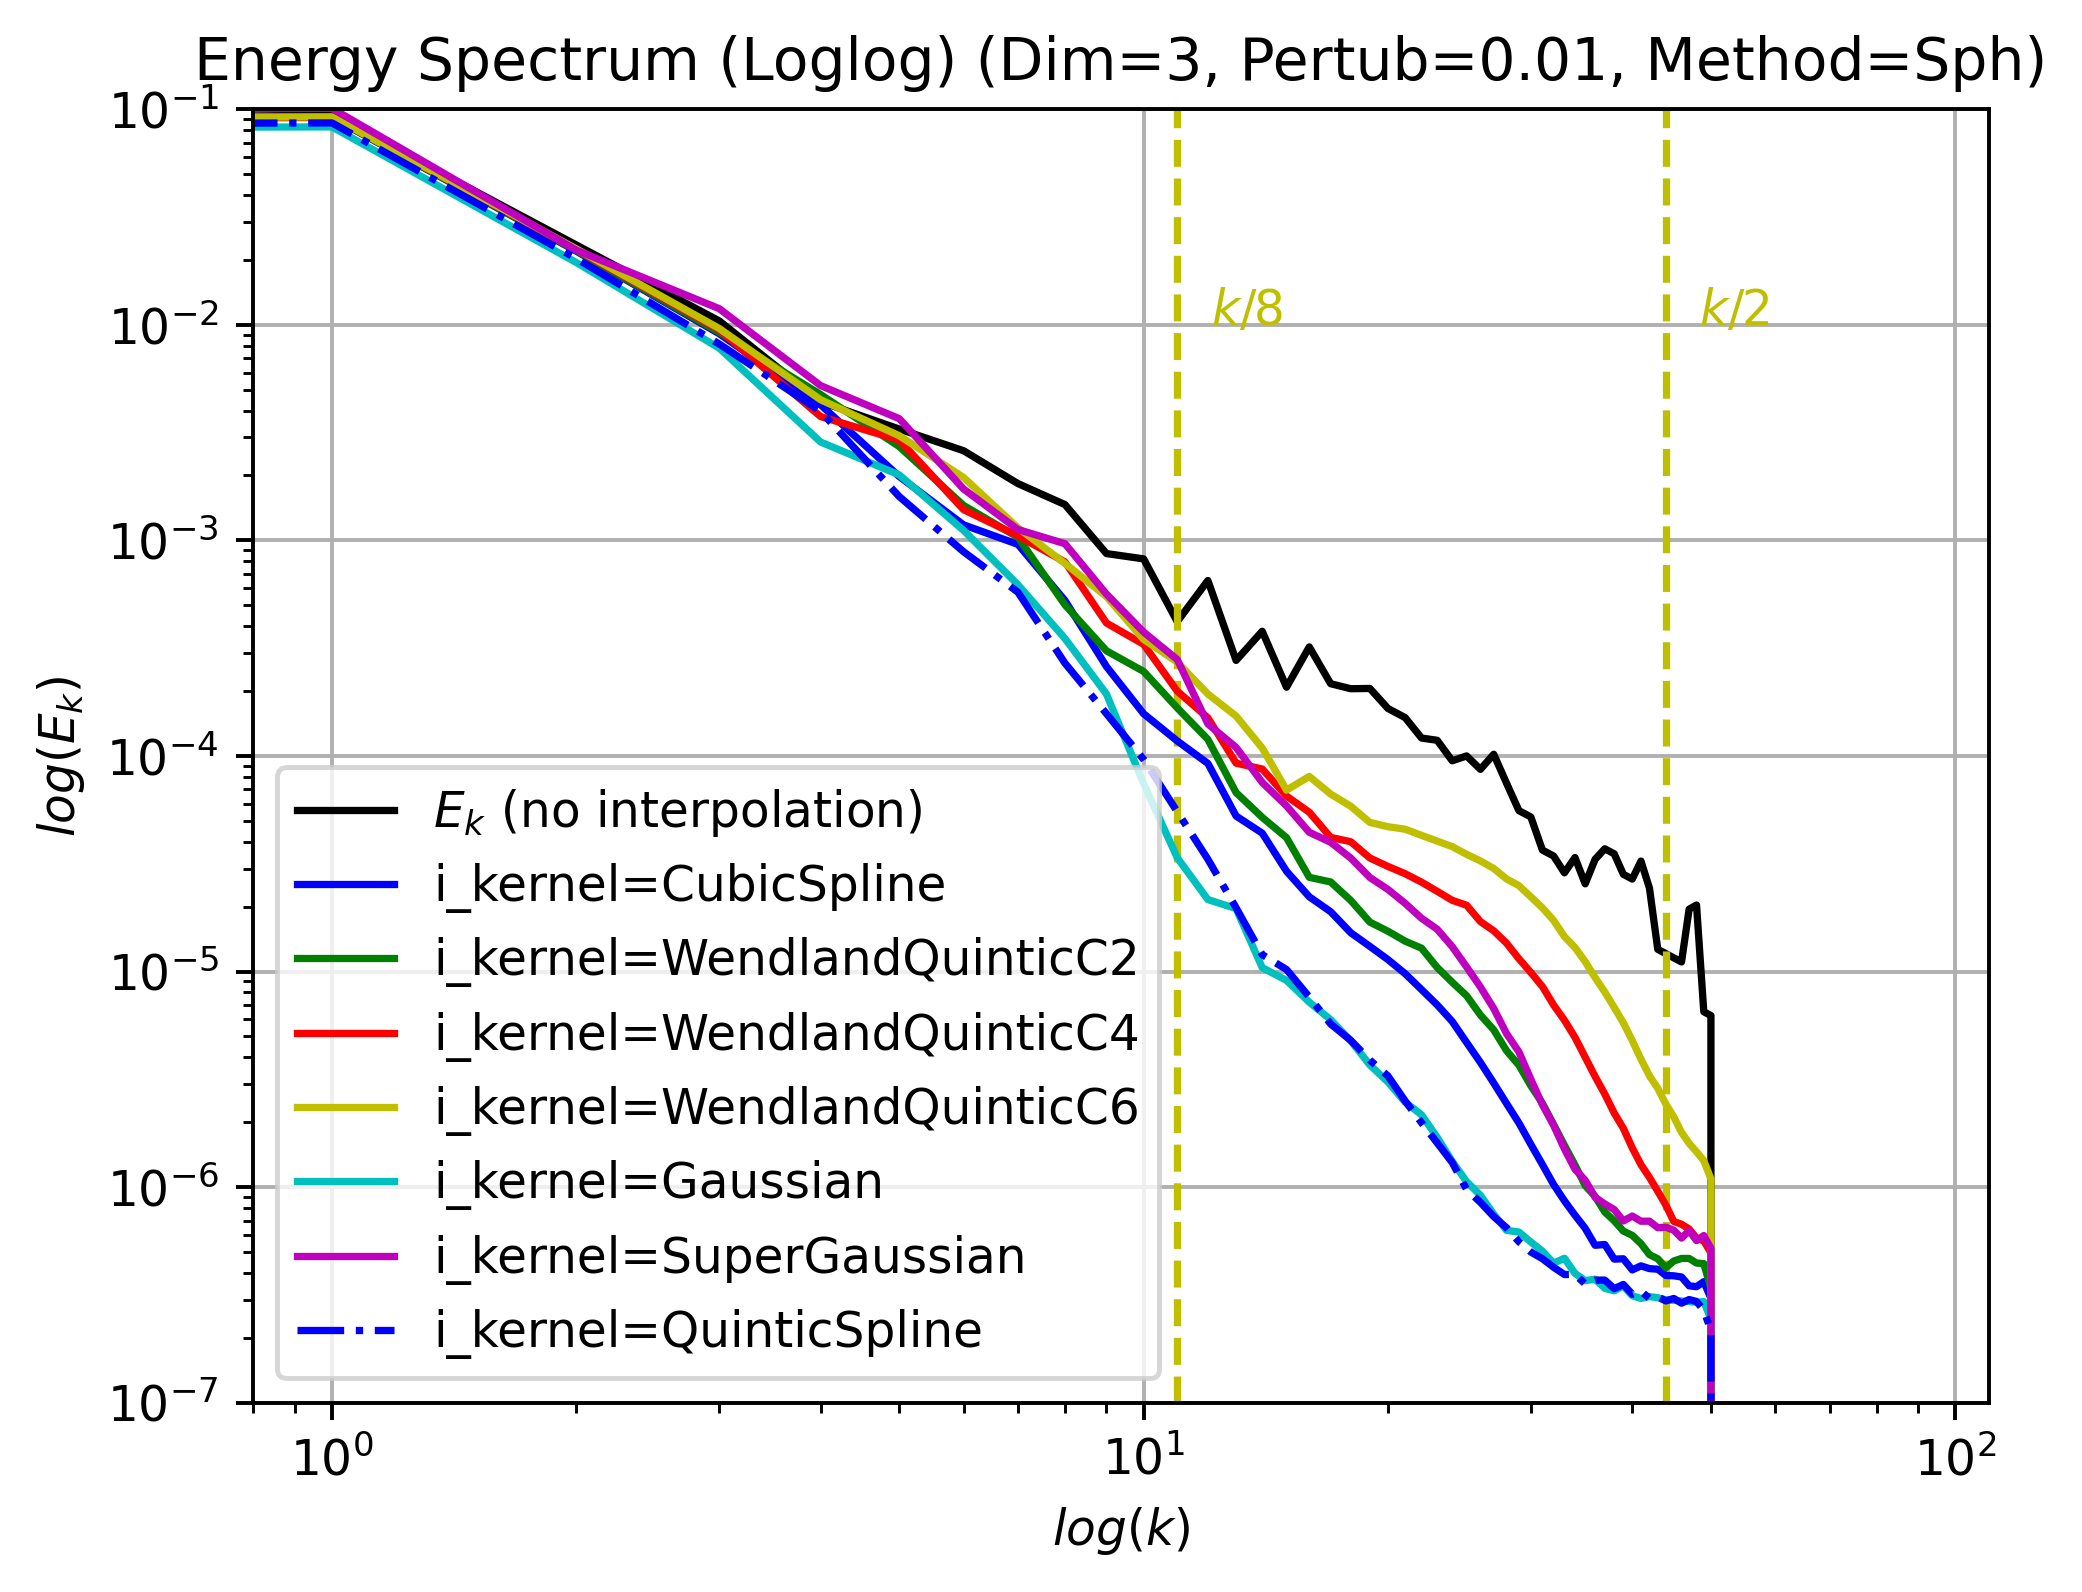
\includegraphics[width=6cm]{Code-Figures/sin-vel-prof-i-kernel/Energy Spectrum (Loglog) (Dim=3, Pertub=0.01, Method=Sph).png}
		\caption{$3D$ $E(k)$ field}
	\end{subfigure}
	\caption{The scalar fields $E(k)$ for $1D$, $2D$, and $3D$ case, for various interpolation kernels.}
	\label{fig:espec-scalar-fields-i-kernels}
\end{figure}

Finally, in order to measure the effect of particle resolution on the computed energy spectrum, test-cases with a $\gamma=1$ and $N=30$ were considered for all dimensions, with the range of number of particles along each axis being $[61, 91, 121]$.
From the results shown in \figref{fig:espec-scalar-fields-res}, it can be observed that the energy spectrum computed for the highest resolution, is observed to be the closest to the exact trend, for all dimensions.

\begin{figure}[H]
	\begin{subfigure}{7cm}
		\centering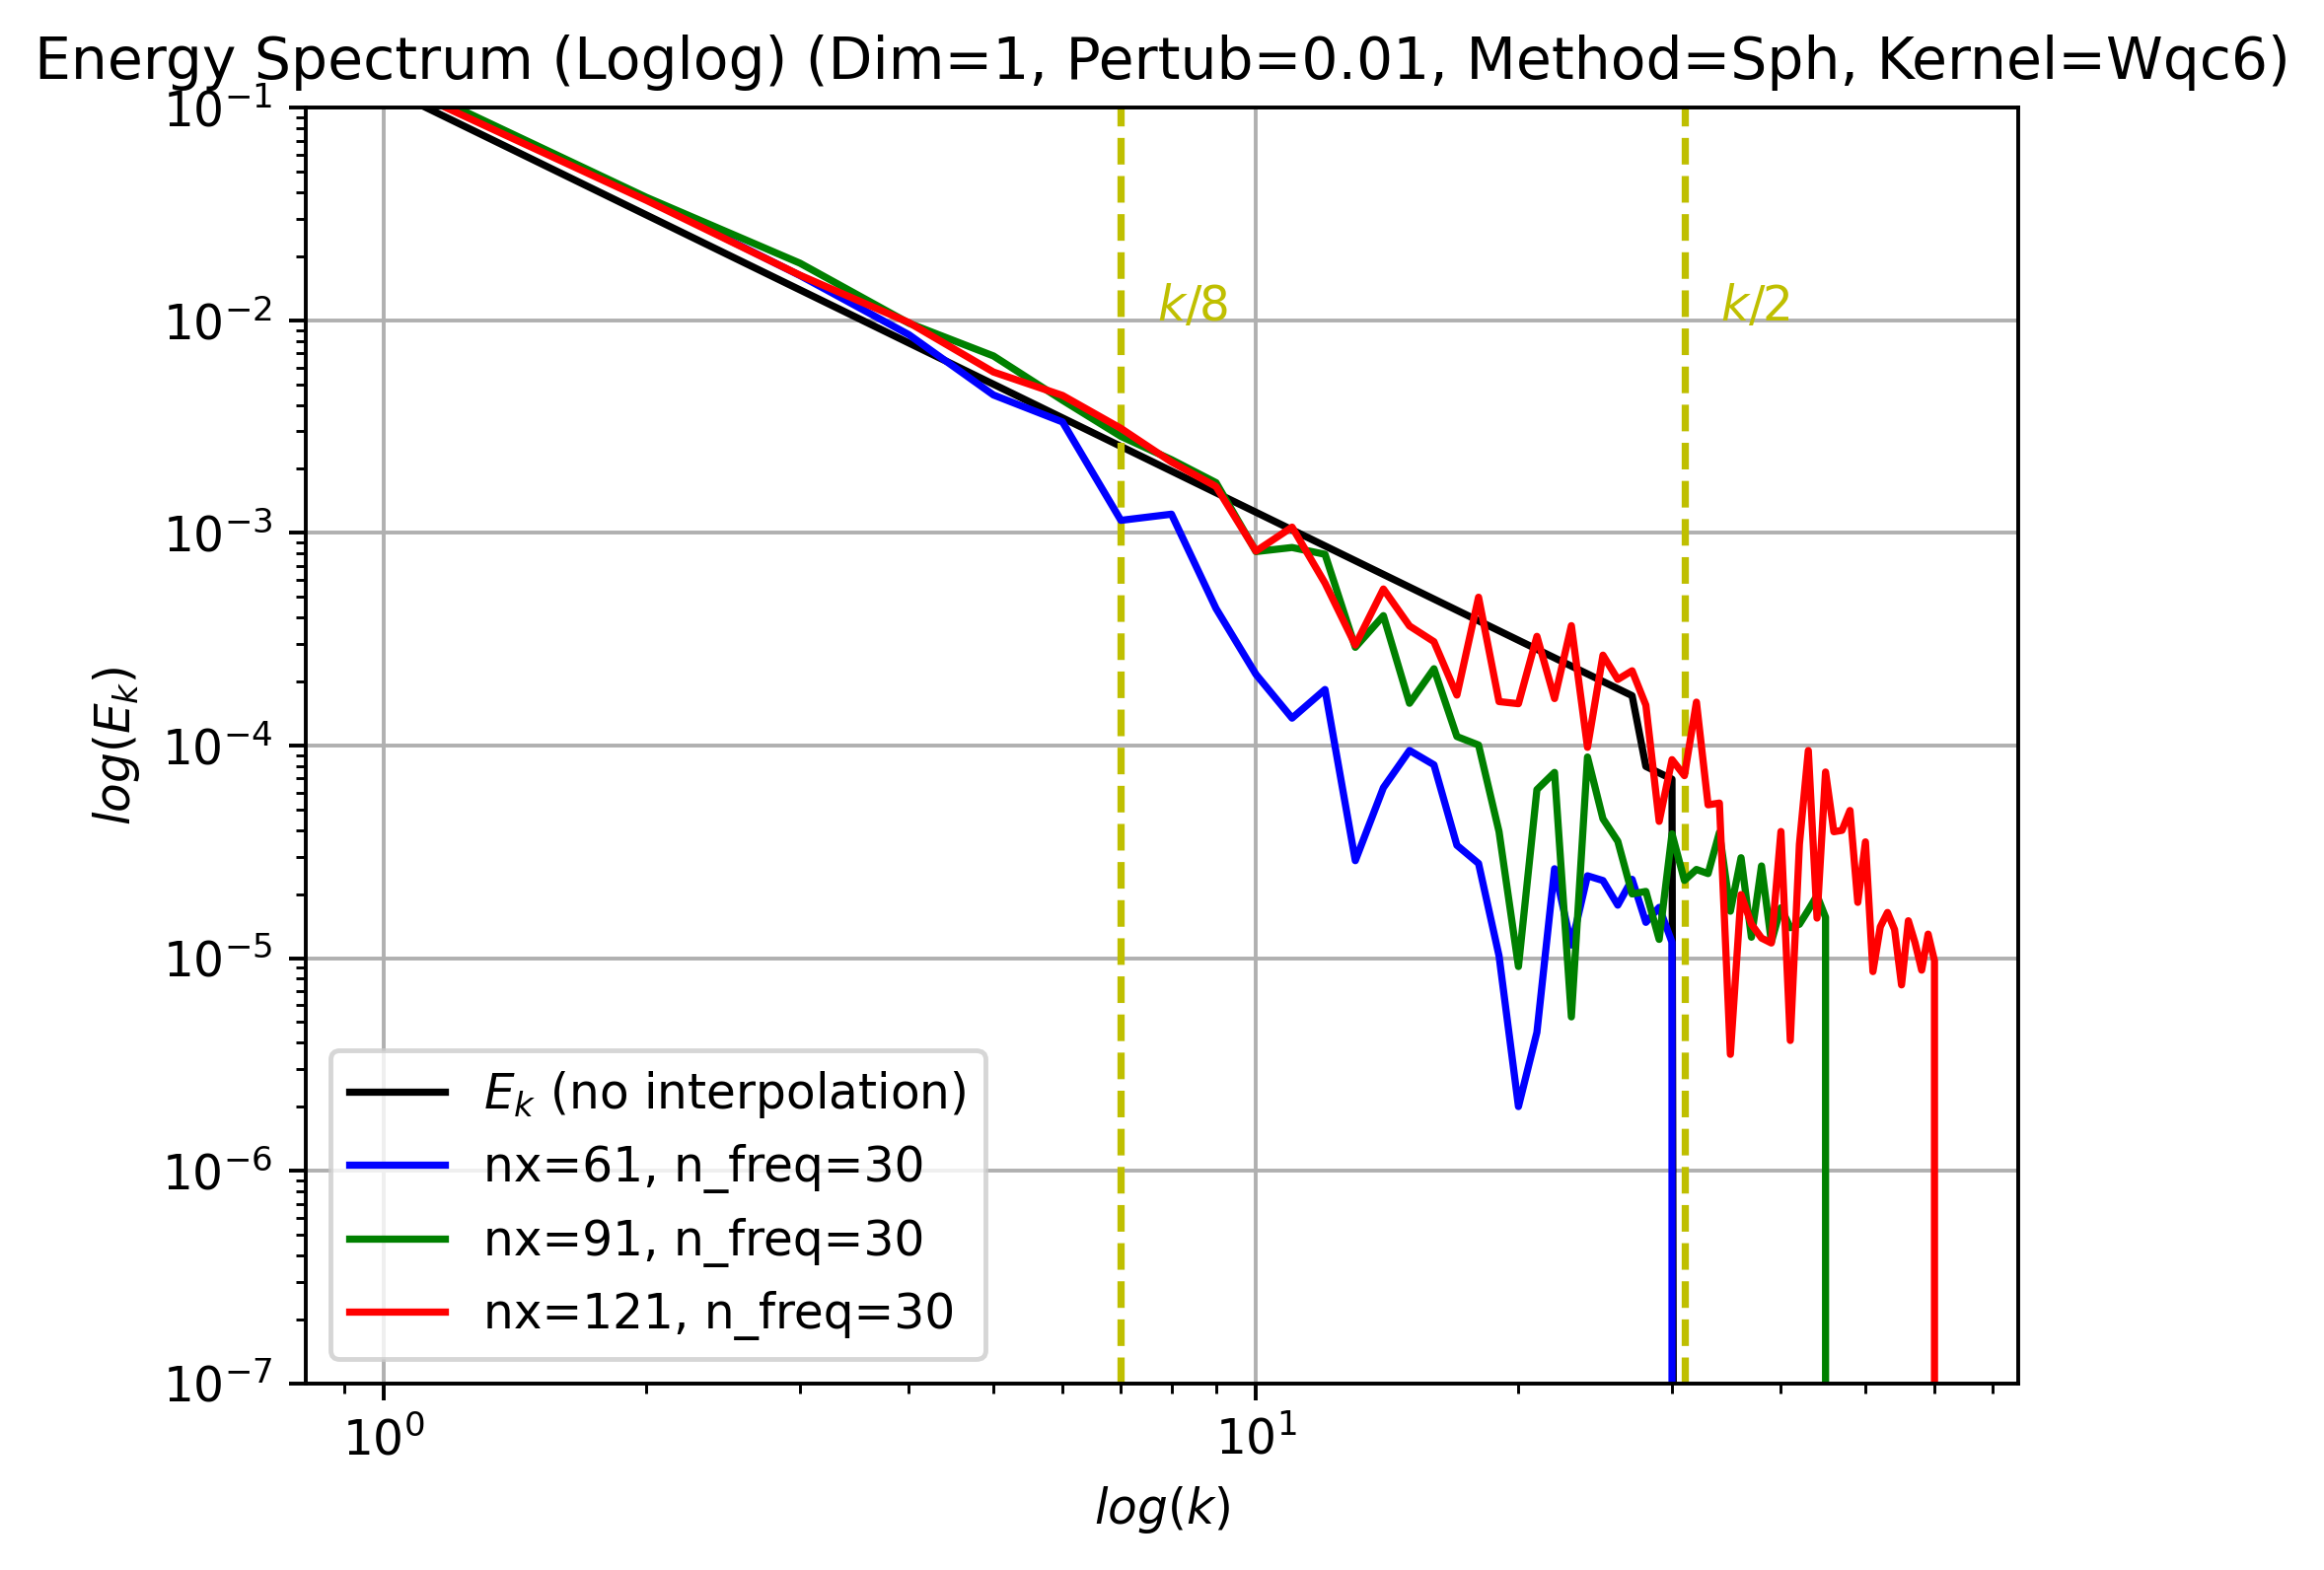
\includegraphics[width=6cm]{Code-Figures/sin-vel-prof-res/Energy Spectrum (Loglog) (Dim=1, Pertub=0.01, Method=Sph, Kernel=Wqc6).png}
		\caption{$1D$ $E(k)$ field}
	\end{subfigure}
	\begin{subfigure}{7cm}
		\centering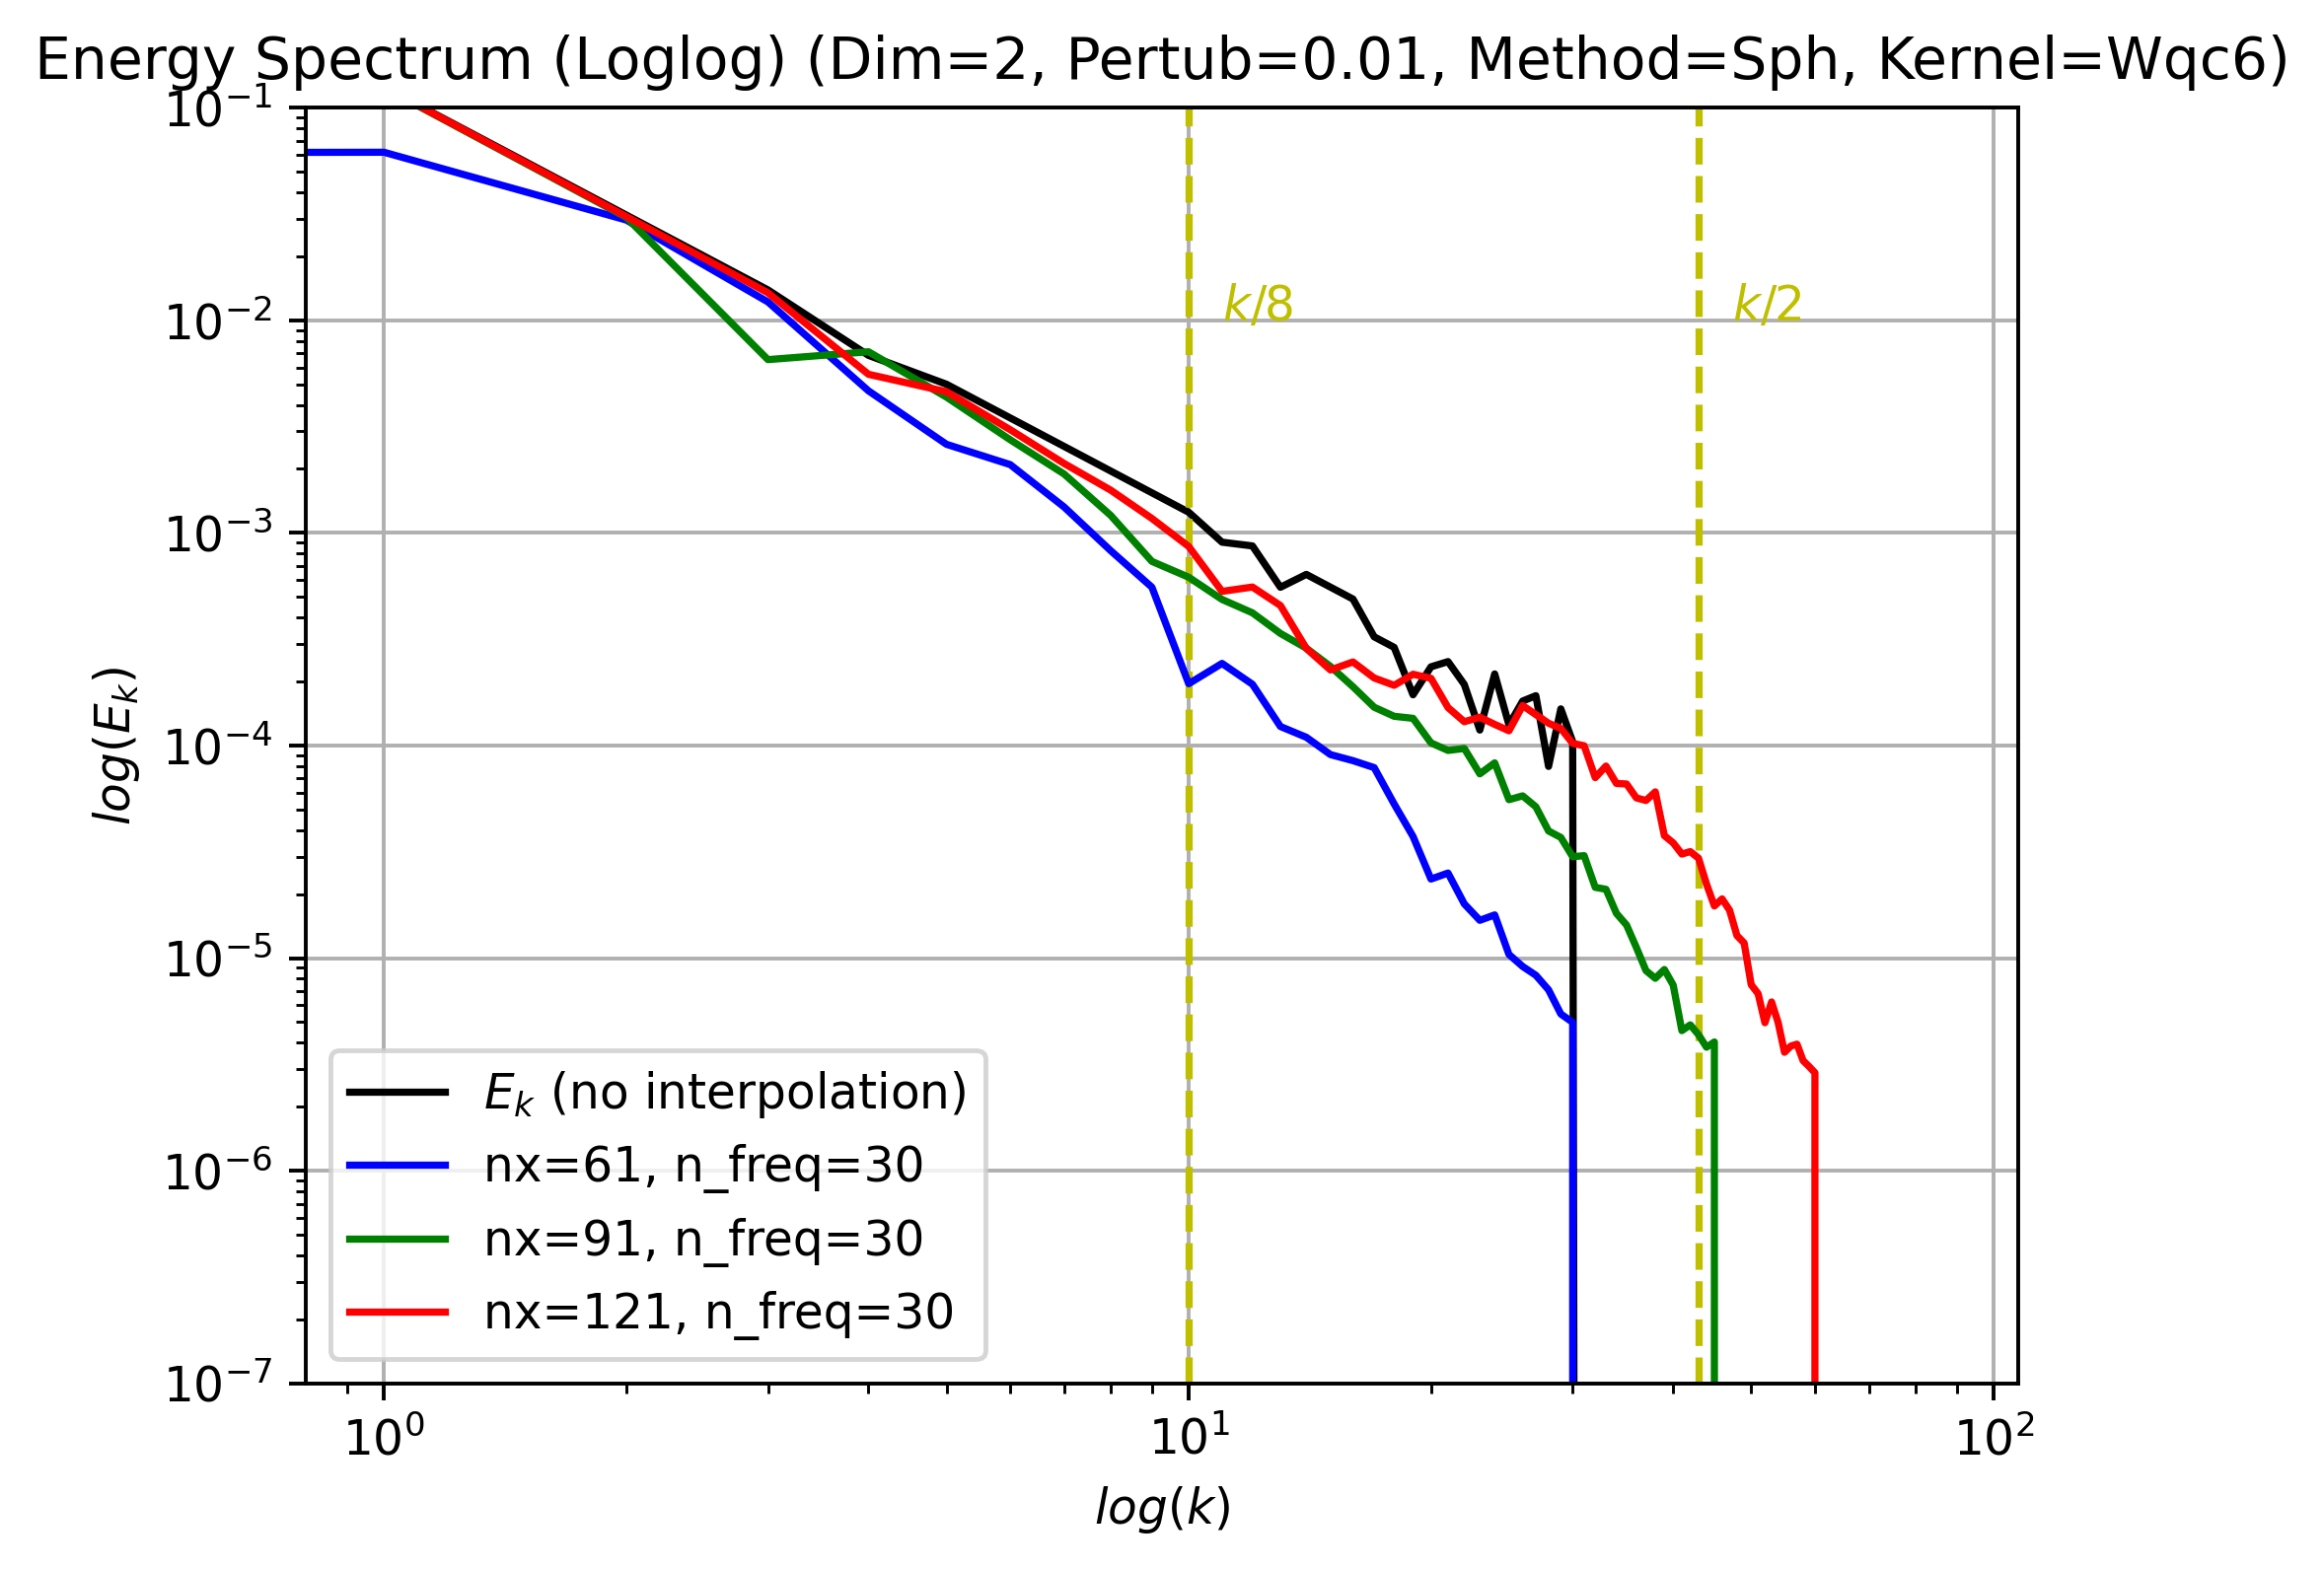
\includegraphics[width=6cm]{Code-Figures/sin-vel-prof-res/Energy Spectrum (Loglog) (Dim=2, Pertub=0.01, Method=Sph, Kernel=Wqc6).png}
		\caption{$2D$ $E(k)$ field}
	\end{subfigure}
	\begin{subfigure}{7cm}
		\centering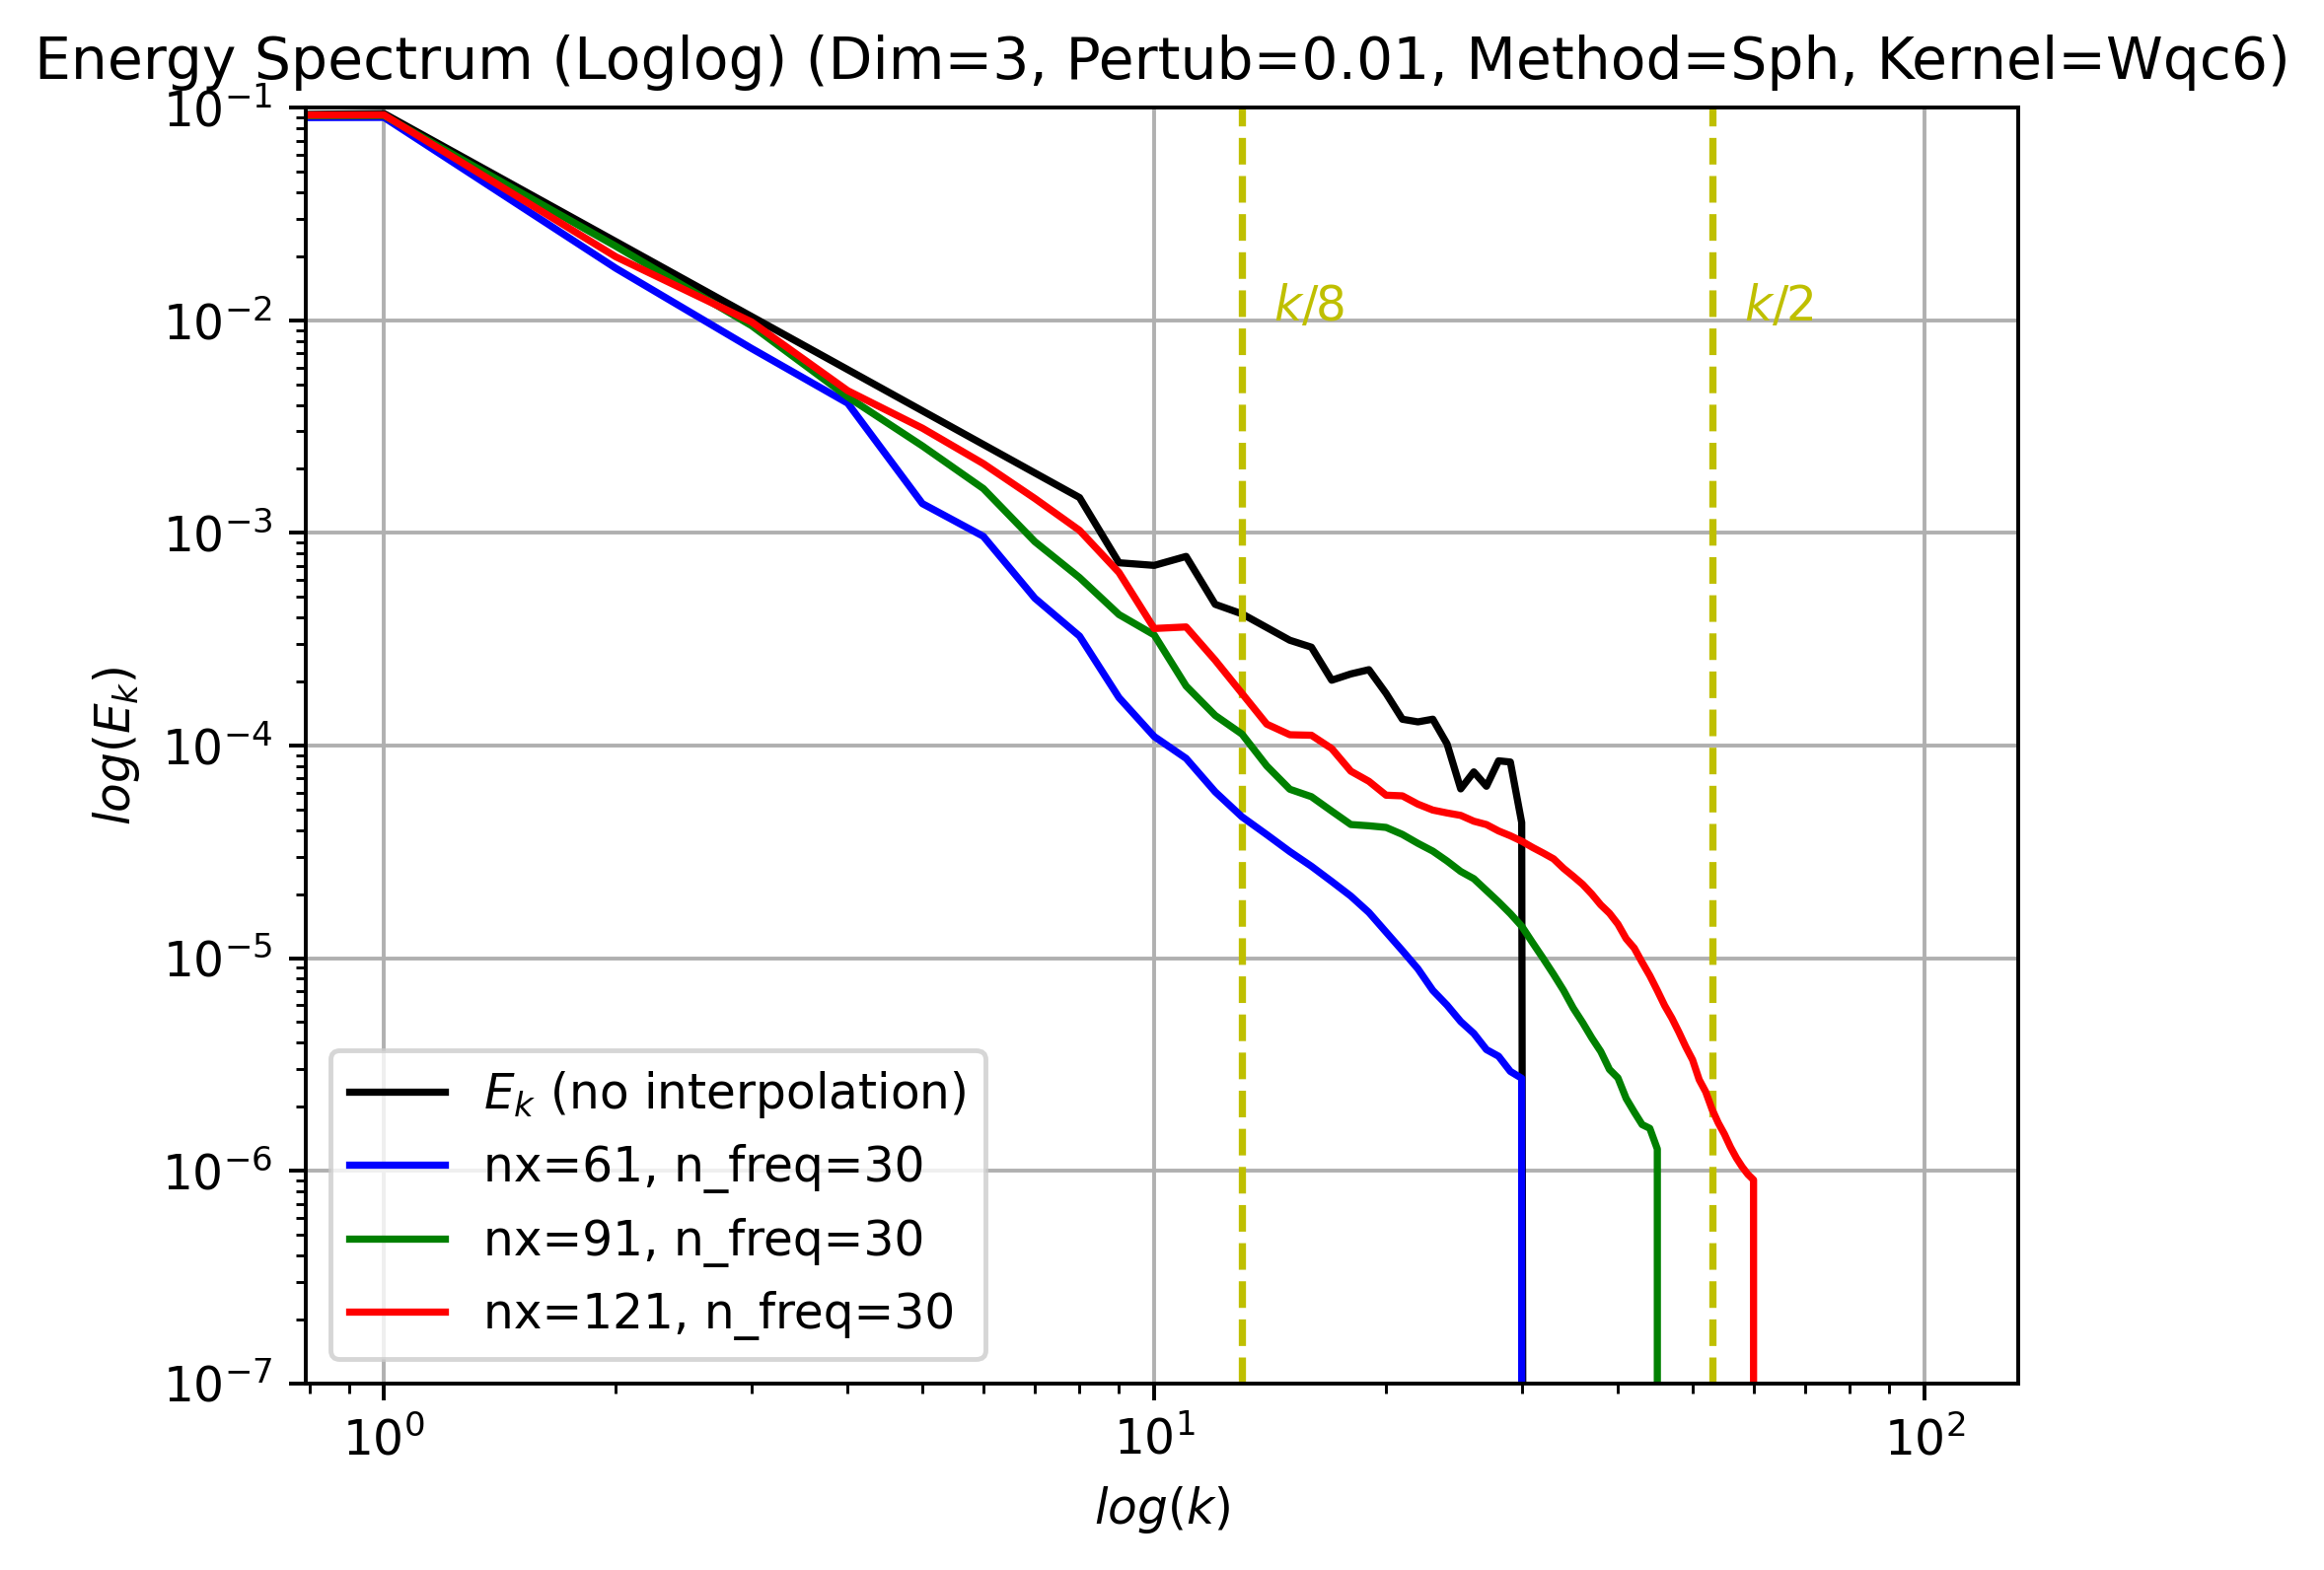
\includegraphics[width=6cm]{Code-Figures/sin-vel-prof-res/Energy Spectrum (Loglog) (Dim=3, Pertub=0.01, Method=Sph, Kernel=Wqc6).png}
		\caption{$3D$ $E(k)$ field}
	\end{subfigure}
	\caption{The scalar fields $E(k)$ for $1D$, $2D$, and $3D$ case, for various particle resolutions.}
	\label{fig:espec-scalar-fields-res}
\end{figure}


\subsection{Finite-time Lyapunov Exponent (FTLE) Field}

In order to compute the FTLE field, the flow field, at two different time instances is required, i.e., $t_i$ and $t_f$.
The flow field corresponding to the earlier time instance is stored in the \texttt{initial} particle array, while the flow field corresponding to the later time instance is stored in the \texttt{final} particle array.

The forward-in-time (FIT) FTLE field is calculated as defined in the work of \cite{sun2016detection}:
\begin{equation}
	\lambda_{t_i}^{t_f}(\vect{x}) = \frac{1}{\abs{t_f - t_i}} \ln \bigg( \sqrt{\Lambda_{max}[ \mathbb{C}_{t_i}^{t_f}(\vect{x}) ]}  \bigg),
\end{equation}
\begin{equation}
  \mathbb{C}_{t_i}^{t_f}(\vect{x}) = \mathbb{F}_{t_i}^{t_f}(\vect{x})^T \mathbb{F}_{t_i}^{t_f}(\vect{x}),
\end{equation}
where, $\mathbb{F}_{t_i}^{t_f}(\vect{x})$ is the deformation gradient tensor, and $\Lambda_{max}$ is the maximum eigenvalue of the Cauchy-Green tensor $\mathbb{C}_{t_i}^{t_f}(\vect{x})$. Correspondingly, the backward-in-time (BIT) FTLE field is calculated as:
\begin{equation}
  \lambda_{t_f}^{t_i}(\vect{x}) = \frac{1}{\abs{t_f - t_i}} \ln \bigg( \sqrt{ \frac{1}{\Lambda_{min}[ \mathbb{C}_{t_i}^{t_f}(\vect{x}) ]} }  \bigg).
\end{equation}

The corresponding, SPH approximations for the above equations are:
\begin{equation}
  \mathbb{F}_{t_i}^{t_f}(\vect{x}_i) = \sum_{j} \frac{m_j}{\rho_j} \vect{X}_{ji} \otimes \nabla \mathbb{L}( \vect{x}_i ) \DWIJ,
\end{equation}
\begin{equation}
  \mathbb{L}( \vect{x}_i ) = \bigg[ \sum_j \vect{x}_{ji} \otimes \nabla_i W(\abs{\vect{X}_{ji}}, h_i) \bigg]^{-1},
\end{equation}
where, $(\vect{x}_i, \vect{X}_i)$ corresponds to the initial and final position of the same particle.

In order to test the correctness of the FTLE field computation, the following test-cases were devised.
\begin{itemize}
  \item \texttt{parabolic}
  \begin{equation}
    X = 1.5x, \quad Y = x^2 + y,
  \end{equation}

  \item \texttt{spiral}
  \begin{equation}
    X = x + 0.1 \cos(2 \pi r^2), \quad Y = y + 0.1 \sin(2 \pi r^2), \quad r = \sqrt{x^2 + y^2},
    \end{equation}
\end{itemize}

\begin{figure}[H]
		\centering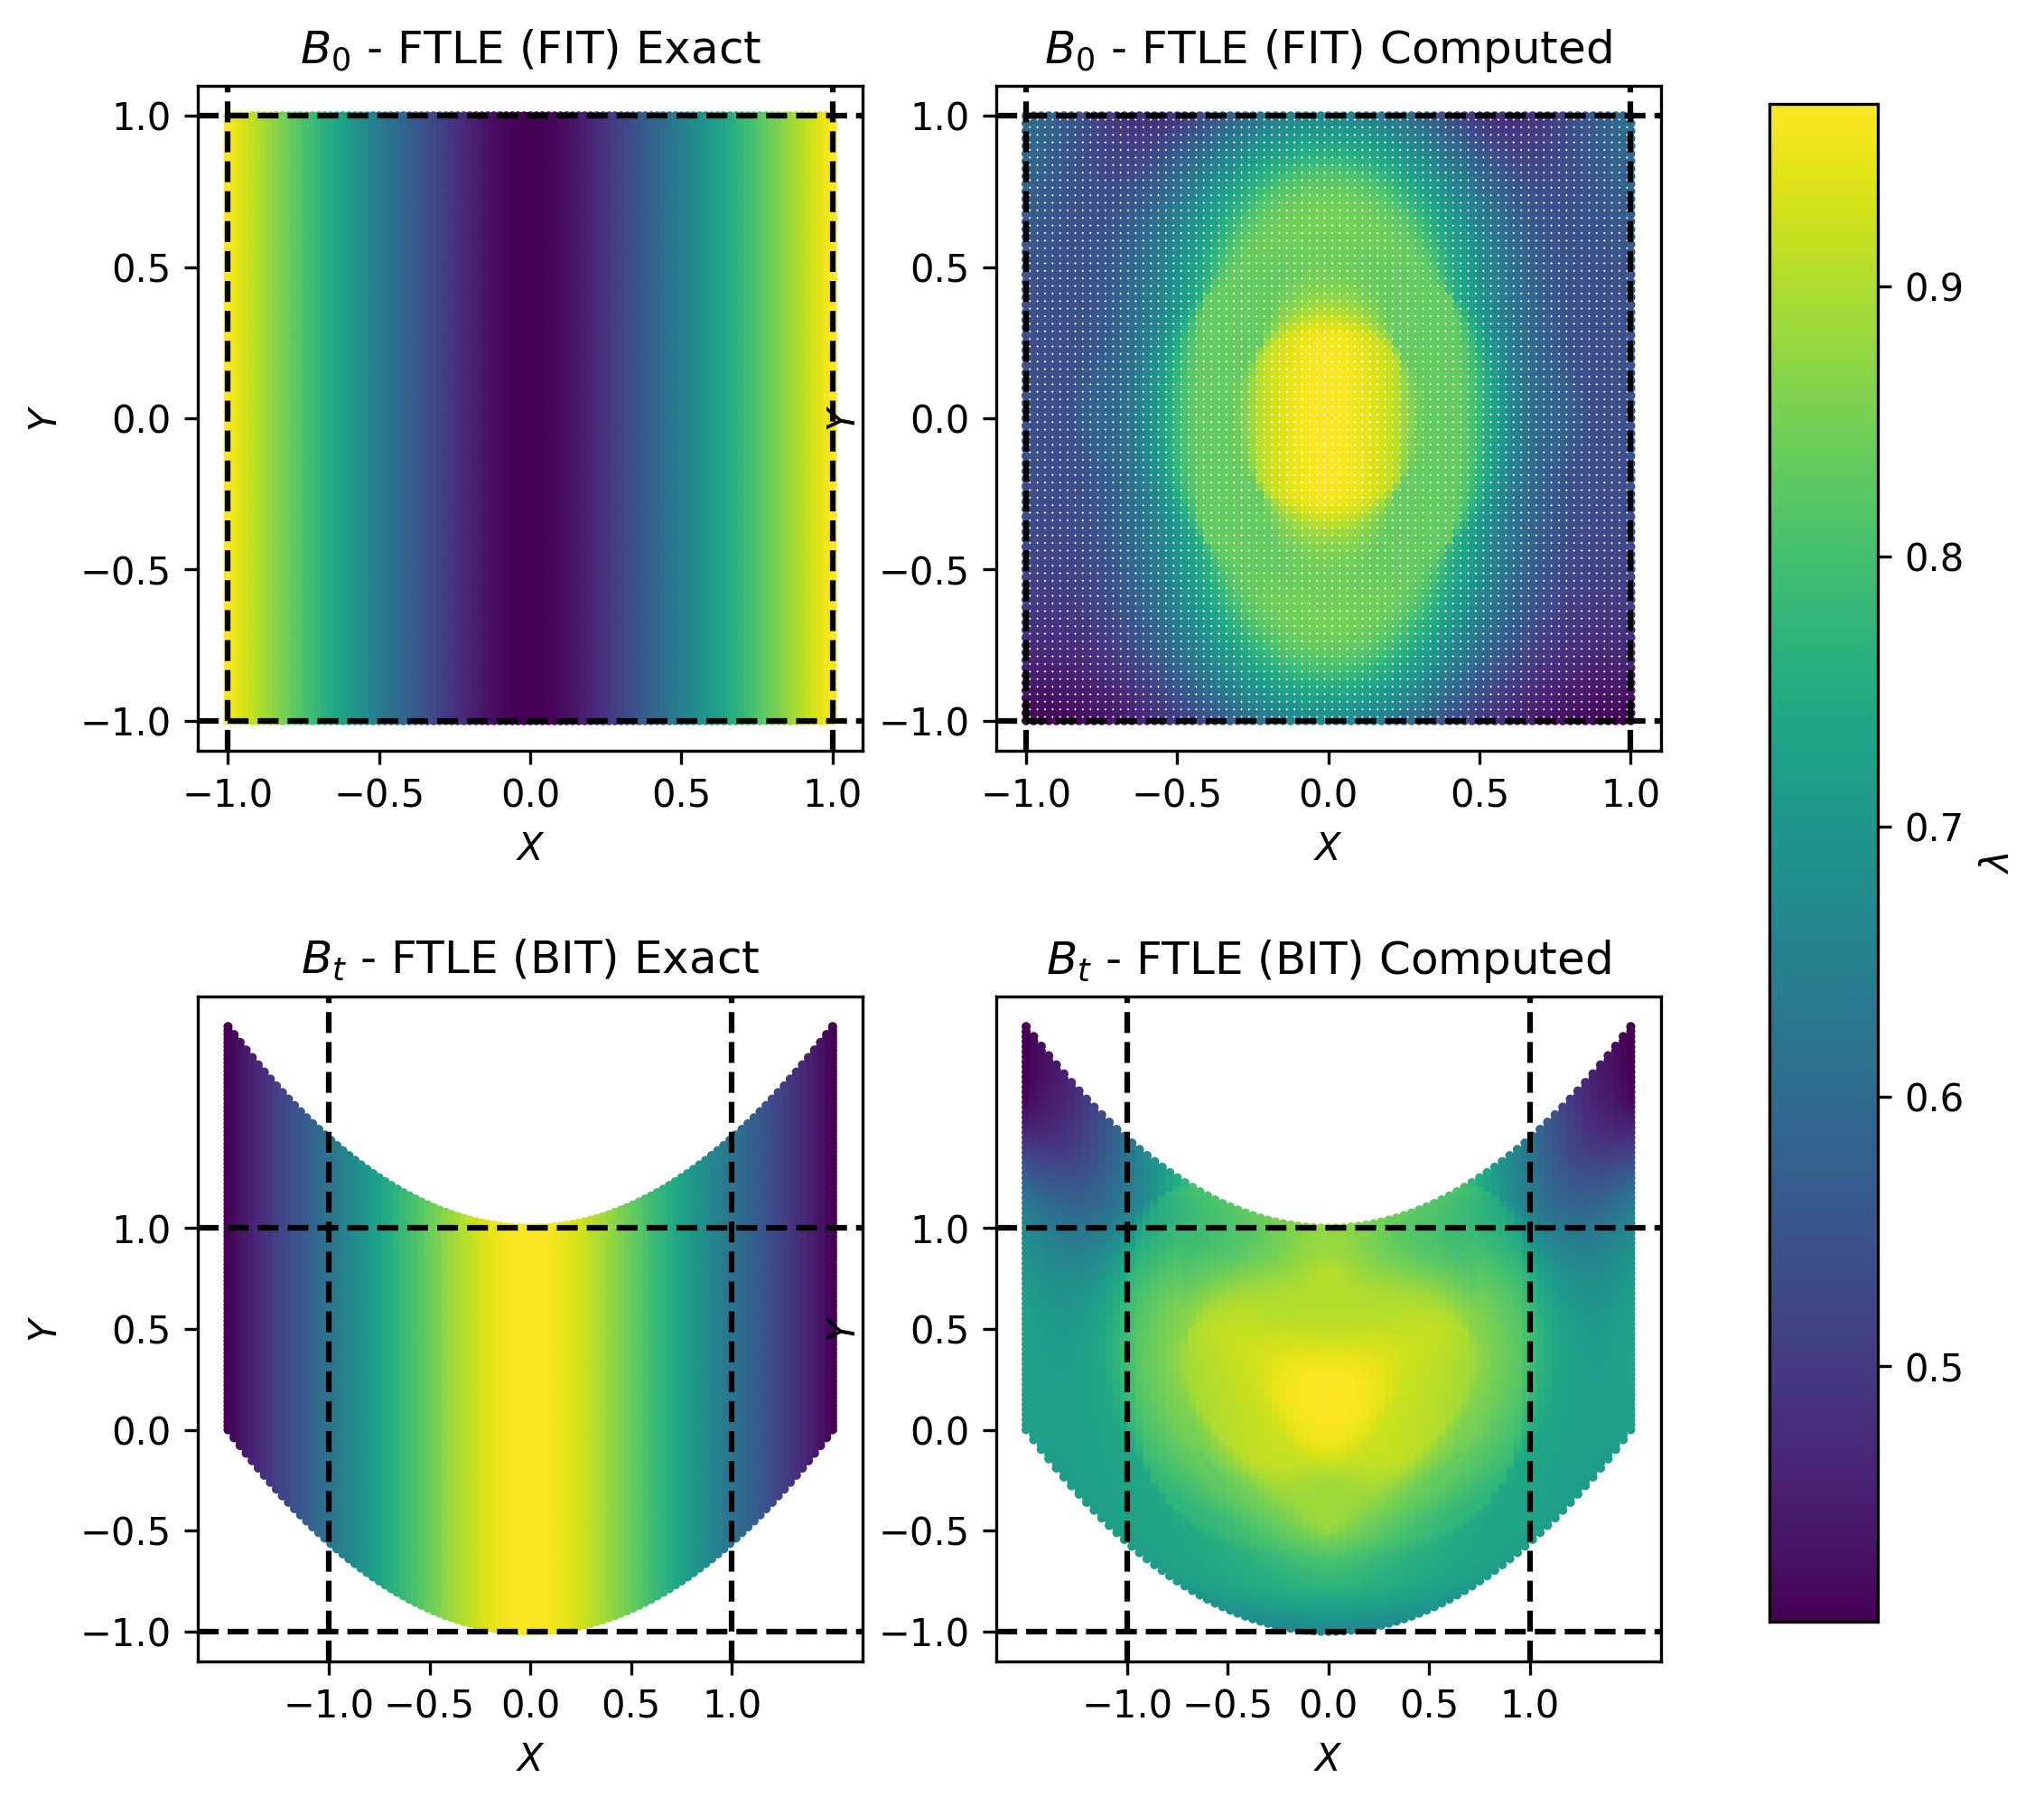
\includegraphics[width=10cm]{Code-Figures/ftle_parabolic.png}
		\caption{Parabolic displacement field}
    \label{fig:ftle-parabolic}
\end{figure}
\begin{figure}[H]
  \centering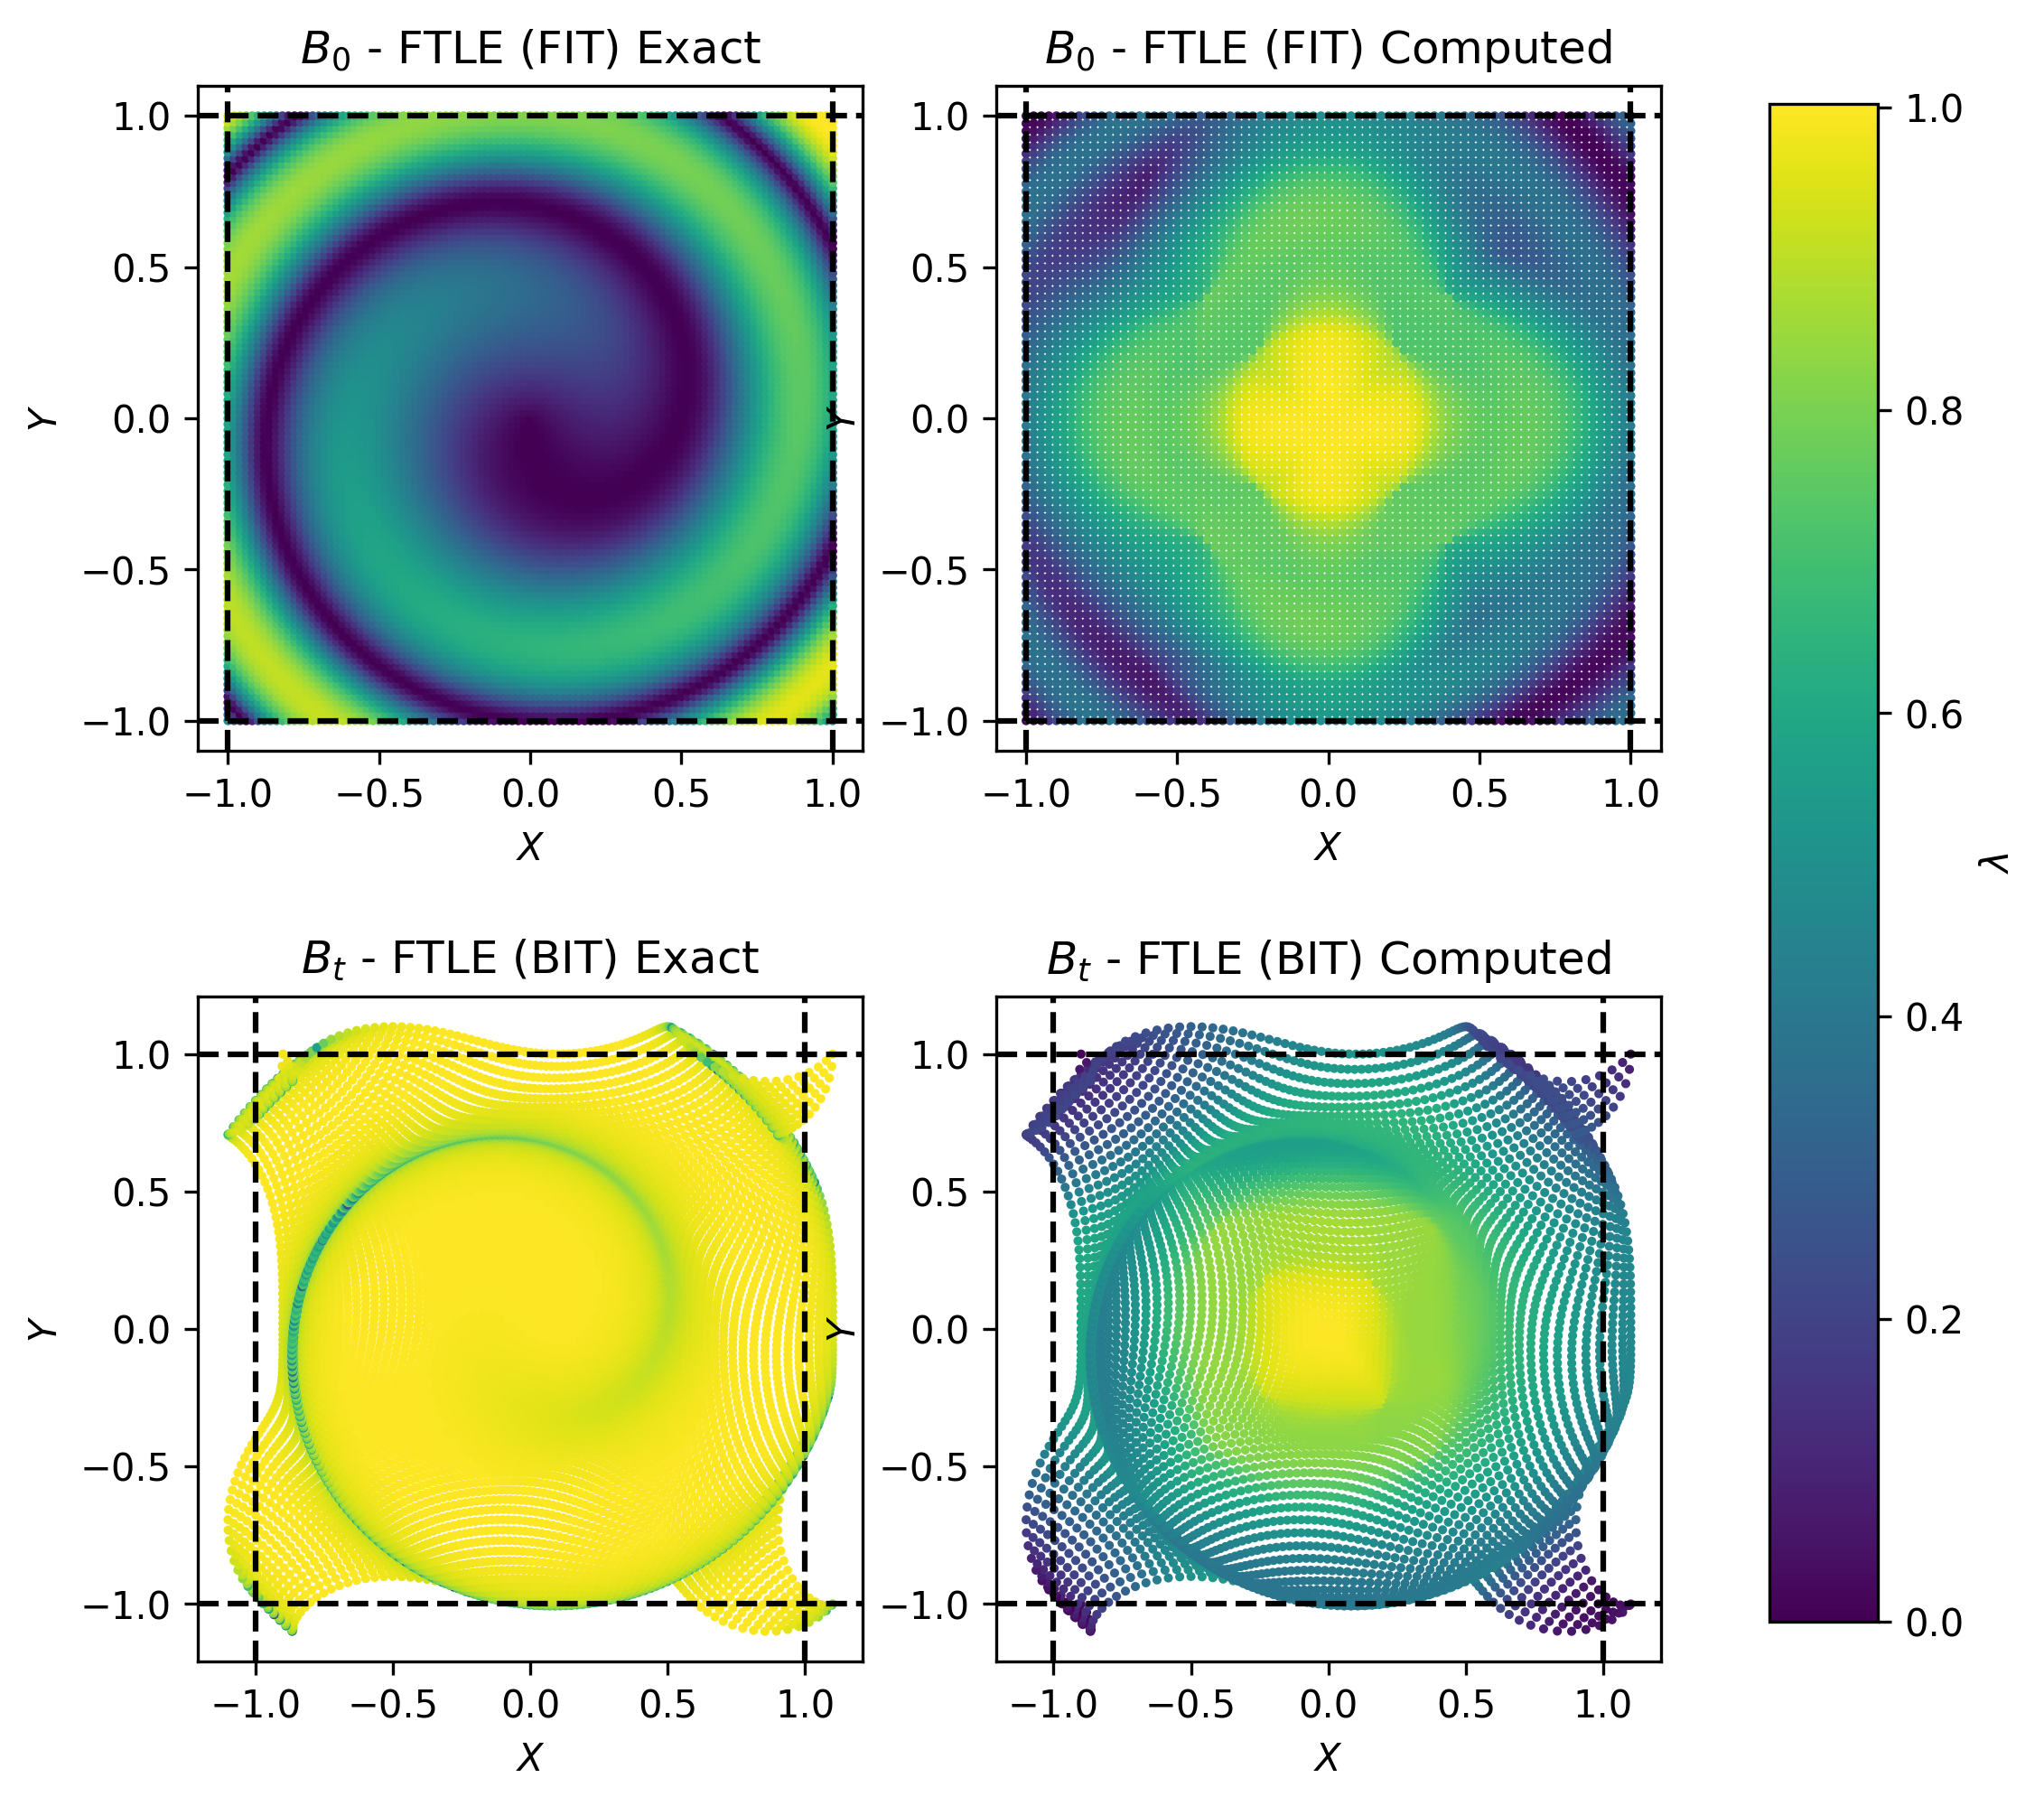
\includegraphics[width=10cm]{Code-Figures/ftle_spiral.png}
  \caption{Spiral displacement field}
  \label{fig:ftle-spiral}
\end{figure}

As seen in \figref{fig:ftle-parabolic} and \figref{fig:ftle-spiral} ($B_0$: initial configuration, $B_t$: final configuration), it can be observed that although the FTLE fields can to an extent qualitatively capture the evolution of the configurations, i.e, attracting/repelling pathlines, it is however, not as accurate in terms of actually capturing the exact pathlines. Therefore, it was concluded that in-place of FTLE fields, tracer particles can be used to visualize the flow field, which would be more accurate in terms of capturing the exact pathlines, but would be computationally more expensive, since the tracer particles would have to be advected along with the flow field, and would also require additional post-processing to visualize the pathlines. They would also have to be done in-situ, i.e., during the simulation itself, as opposed to the FTLE fields, which can be computed post-simulation or in-situ as well.
% TODO: iPad fig of atracting and repelling pathlines


\section{Turbulence Modelling}
\subsection{Implementation of models}
A broad classification of the major categories of turbulence models, has already been discussed in \chapref{chap:turbulence-modelling}.
In order to better understand the nature of each major categories, and to subsequently understand the implementation of the same, a select few representative schemes from each of these models are considered, which are listed in \tabref{tab:rep-turb-models}.

\begin{table}[ht!]
  \centering
  \resizebox{\textwidth}{!}{%
  \begin{tabular}{|l|l|l|l|}
  \hline
  \multicolumn{1}{|c|}{\textbf{Turbulence Model}} & \multicolumn{1}{c|}{\textbf{Section}} & \multicolumn{1}{c|}{\textbf{Scheme Name}}                                                                               & \multicolumn{1}{c|}{\textbf{Reference}}  \\ \hline
  Viscosity-based Model                           & \secref{sec:visc-based-model}                  & \begin{tabular}[c]{@{}l@{}}Lagrangian with iterative PST and \texttt{coupled\_c} viscosity formulation\\ (L-IPST-C)\end{tabular} & \cite{Negi2022Techniques}            \\ \hline
  Large Eddy Simulation-based Model               & \secref{sec:les-based-model}                   & SPH-LES                                                                                                                          & \cite{Okraschevski2022}              \\ \hline
  Lagrangian LES-based Model                      & \secref{sec:lagrangian-les-based-model}        & $\delta$-LES-SPH                                                                                                                 & \cite{Colagrossi2021QuasiLagrangian} \\ \hline
  RANS-based k-epsilon Model                      & \secref{sec:rans-based-k-epsilon-model}        & $k-\epsilon$ SPH                                                                                                                 & \cite{Shao2006}                      \\ \hline
  LANS-based Model                                & \secref{sec:lans-based-model}                  & SPH-$\epsilon$                                                                                                                   & \cite{Monaghan2017}                  \\ \hline
  \end{tabular}%
  }
  \caption{Implementation of representative turbulence models.}
  \label{tab:rep-turb-models}
\end{table}

In order to test the schemes for SOC, the Taylor-Green vortex problem is chosen. The test-cases are coded using \texttt{automan} \parencite{RamachandranAutoman2018}, which is an open source, Python-based automation framework. All of the simulations run hereafter, are run upto a final time of $t_f=0.1$, with the resolution for each run consisting of $N=[25^2, 50^2, 100^2]$ particles respectively, with the Reynolds number ranging between $Re=[100, 1000, 10000]$ respectively. All of the simulations are run using the \texttt{WendlandQuinticC4} kernel, with a radius multiplier of $2.0$. This choice was based on the work of \cite{Negi2022Techniques}.

The $L_1$ error for each simulation in a run is computed, and plotted against the inverse of the particle spacing, in order to ascertain the order of convergence (OOC) of the scheme. The $L_1$ error at a given time instance is computed as:
\begin{equation}
  L_1(t) = \frac{mean{\abs{\vect{v}^2(t) - \vect{v}^2_{exact}(t)}}}{mean{\abs{\vect{v}^2_{exact}(t)}}},
\end{equation}
where, $\vect{v}(t)$ is the velocity field at time $t$, and $\vect{v}_{exact}(t)$ is the exact velocity field at time $t$.
Subsequently, the $L_1$ error for the entire simulation, is defined as the mean over all the time instances, i.e.,
\begin{equation}
  L_1 = \frac{1}{n_t} \sum_{i=1}^{n_t} L_1(t_i).
\end{equation}

\subsection{L-IPST-C Scheme}

The L-IPST-C scheme was considered over the other viscosity-based schemes, since it was observed to be actually second-order convergent (SOC) by \cite{Negi2022Techniques}, for a wide variety of problems, which included the Gresho vortex problem, Kelvin-Helmholtz instability problem, and the Taylor-Green vortex problem. This scheme considers the weakly-compressible NS equations as the governing equations, and uses the \texttt{coupled\_c} viscosity formulation, which is corrected using the Bonet and Lok correction \parencite{bonet1999variational}. Hence, since the scheme by definition has the viscous term in its governing equation, it does require any additional `artificial'-viscosity term to be added.
The scheme also incorporates the iterative particle shifting technique (IPST) by \cite{Huang_Long_Li_Liu_2019}, in order to redistribute the particles to obtain a reasonably uniform grid of particles in the domain. Besides shifting the position of the particles, the scheme also updates particles' properties such as the density and velocity to keep the approximation of the particle $O(h^2)$.
Based on the parametric study conducted by \cite{Negi2022Techniques}, the proposed scheme is observed to be SOC, by considering the the speed of sound to be $c_s = 20$, and the shifting frequency for the particles through PST to be at every 10 iterations $f_{pst} = 10$.

Since, the study dealt with problems of low $Re$, the scheme was tested for various time-integration schemes from the Runge-Kutta family of integrators, in order to identify their effects, and to subsequently identify the most suitable integrator for problems of high $Re$.
The integrators considered were:
\begin{itemize}
  \item Predict-Evaluate-Correct (\texttt{PEC}),
  \item Runge-Kutta 2 (\texttt{RK2}),
  \item Runge-Kutta 2 with adaptive time-step (\texttt{RK2 Adaptive}),
  \item Runge-Kutta 3 (\texttt{RK3}), and
  \item Runge-Kutta 4 (\texttt{RK4}),
\end{itemize}
with a corresponding $CFL$ values of $[1, 1, 1.5, 2, 2]$ respectively.

\begin{figure}[H]
  \begin{subfigure}{7cm}
    \centering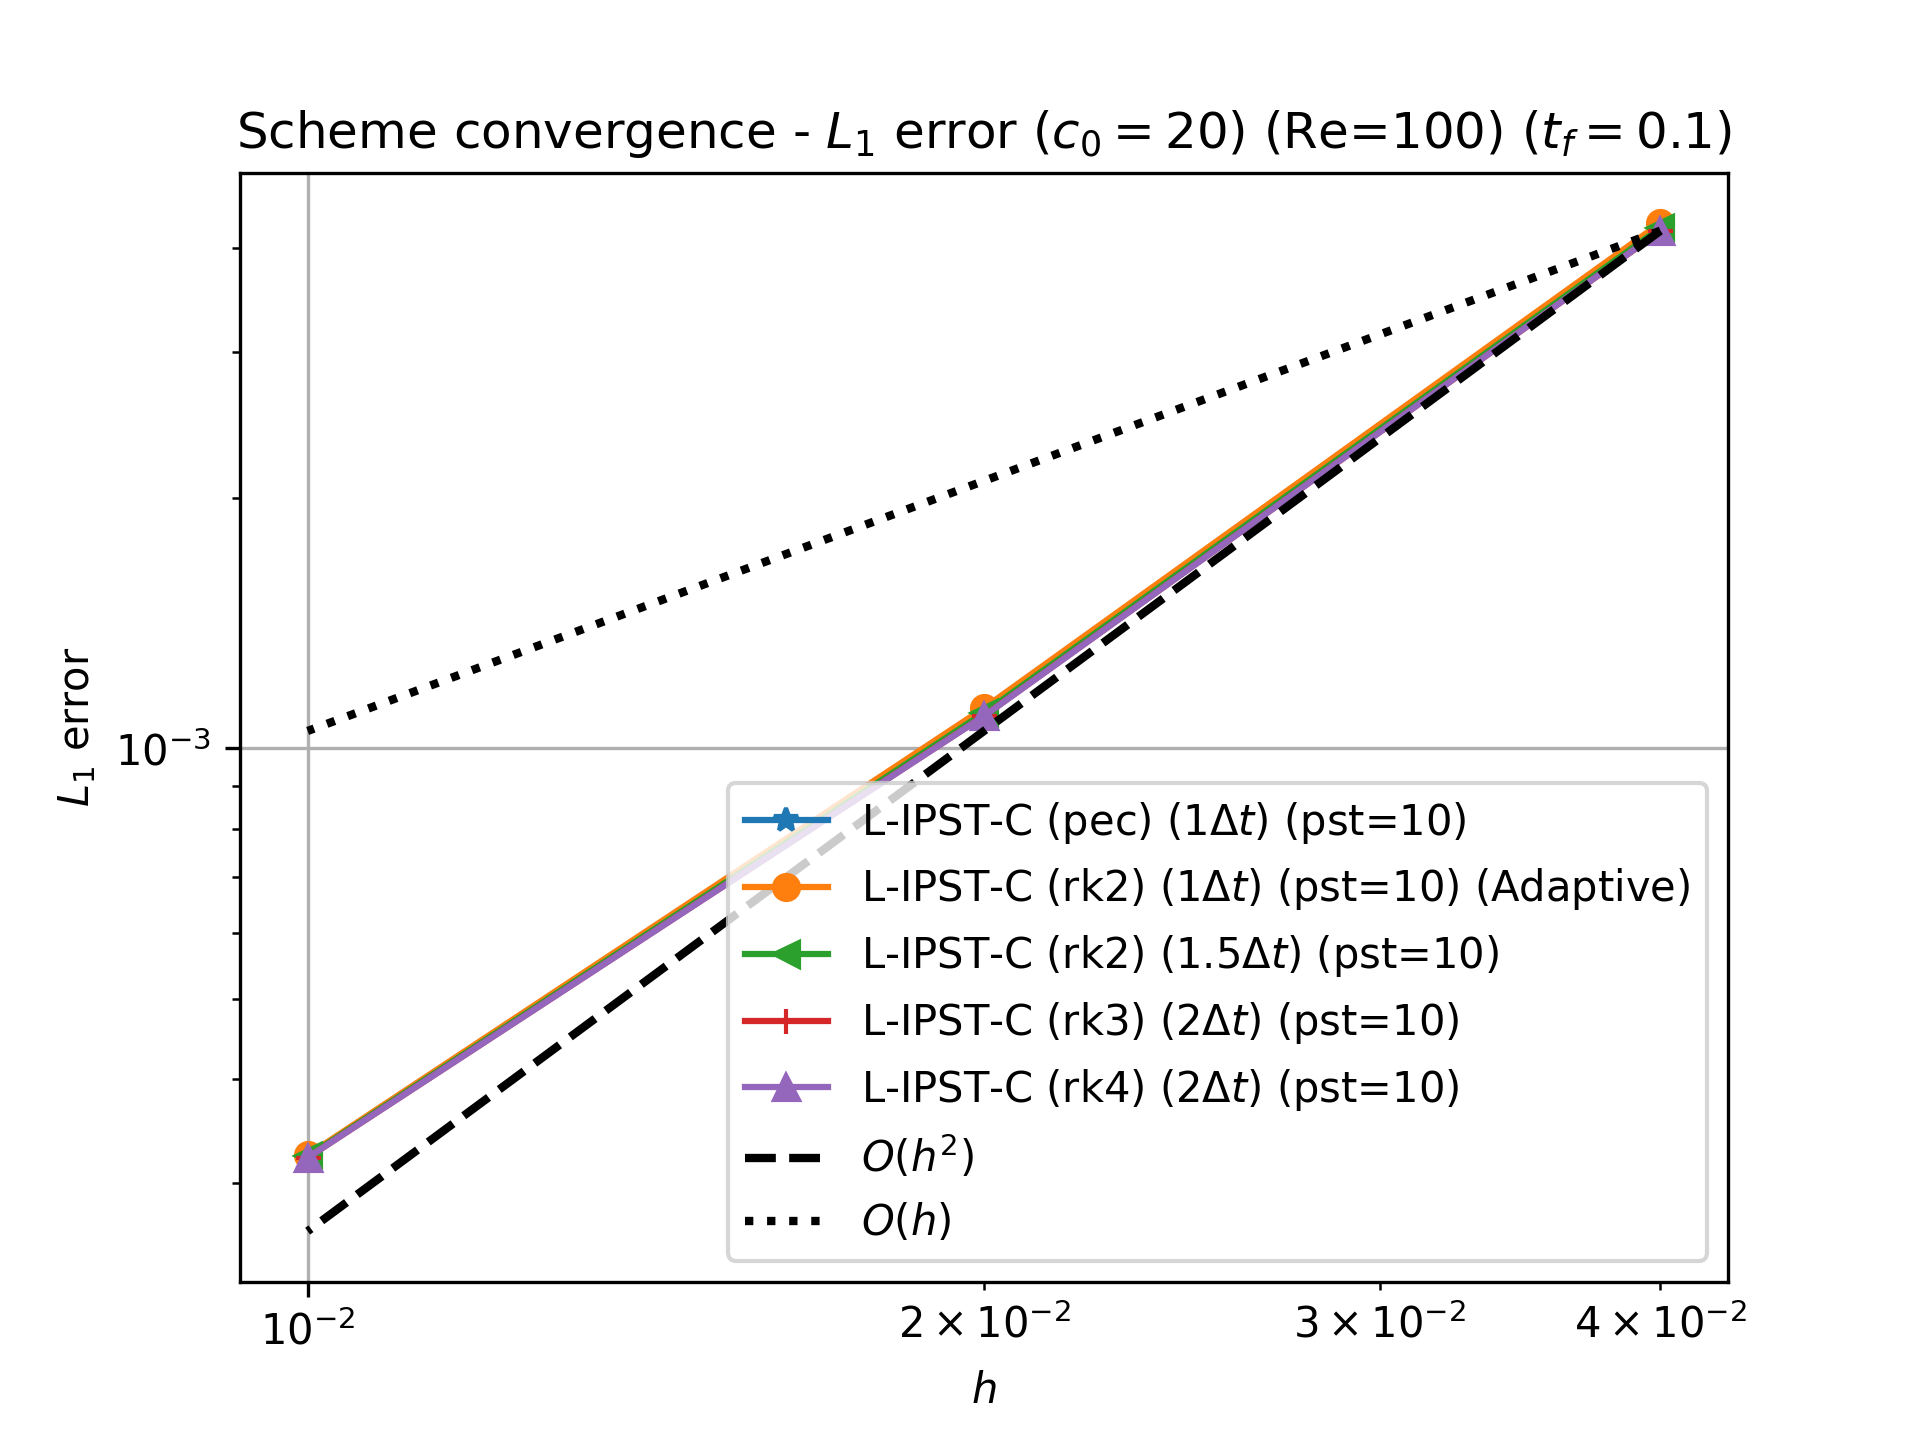
\includegraphics[width=6cm]{Code-Figures/lipstc/integrator/dt_pois_conv_c0_20_re_100.png}
    \caption{$Re = 100$}
  \end{subfigure}
  \begin{subfigure}{7cm}
    \centering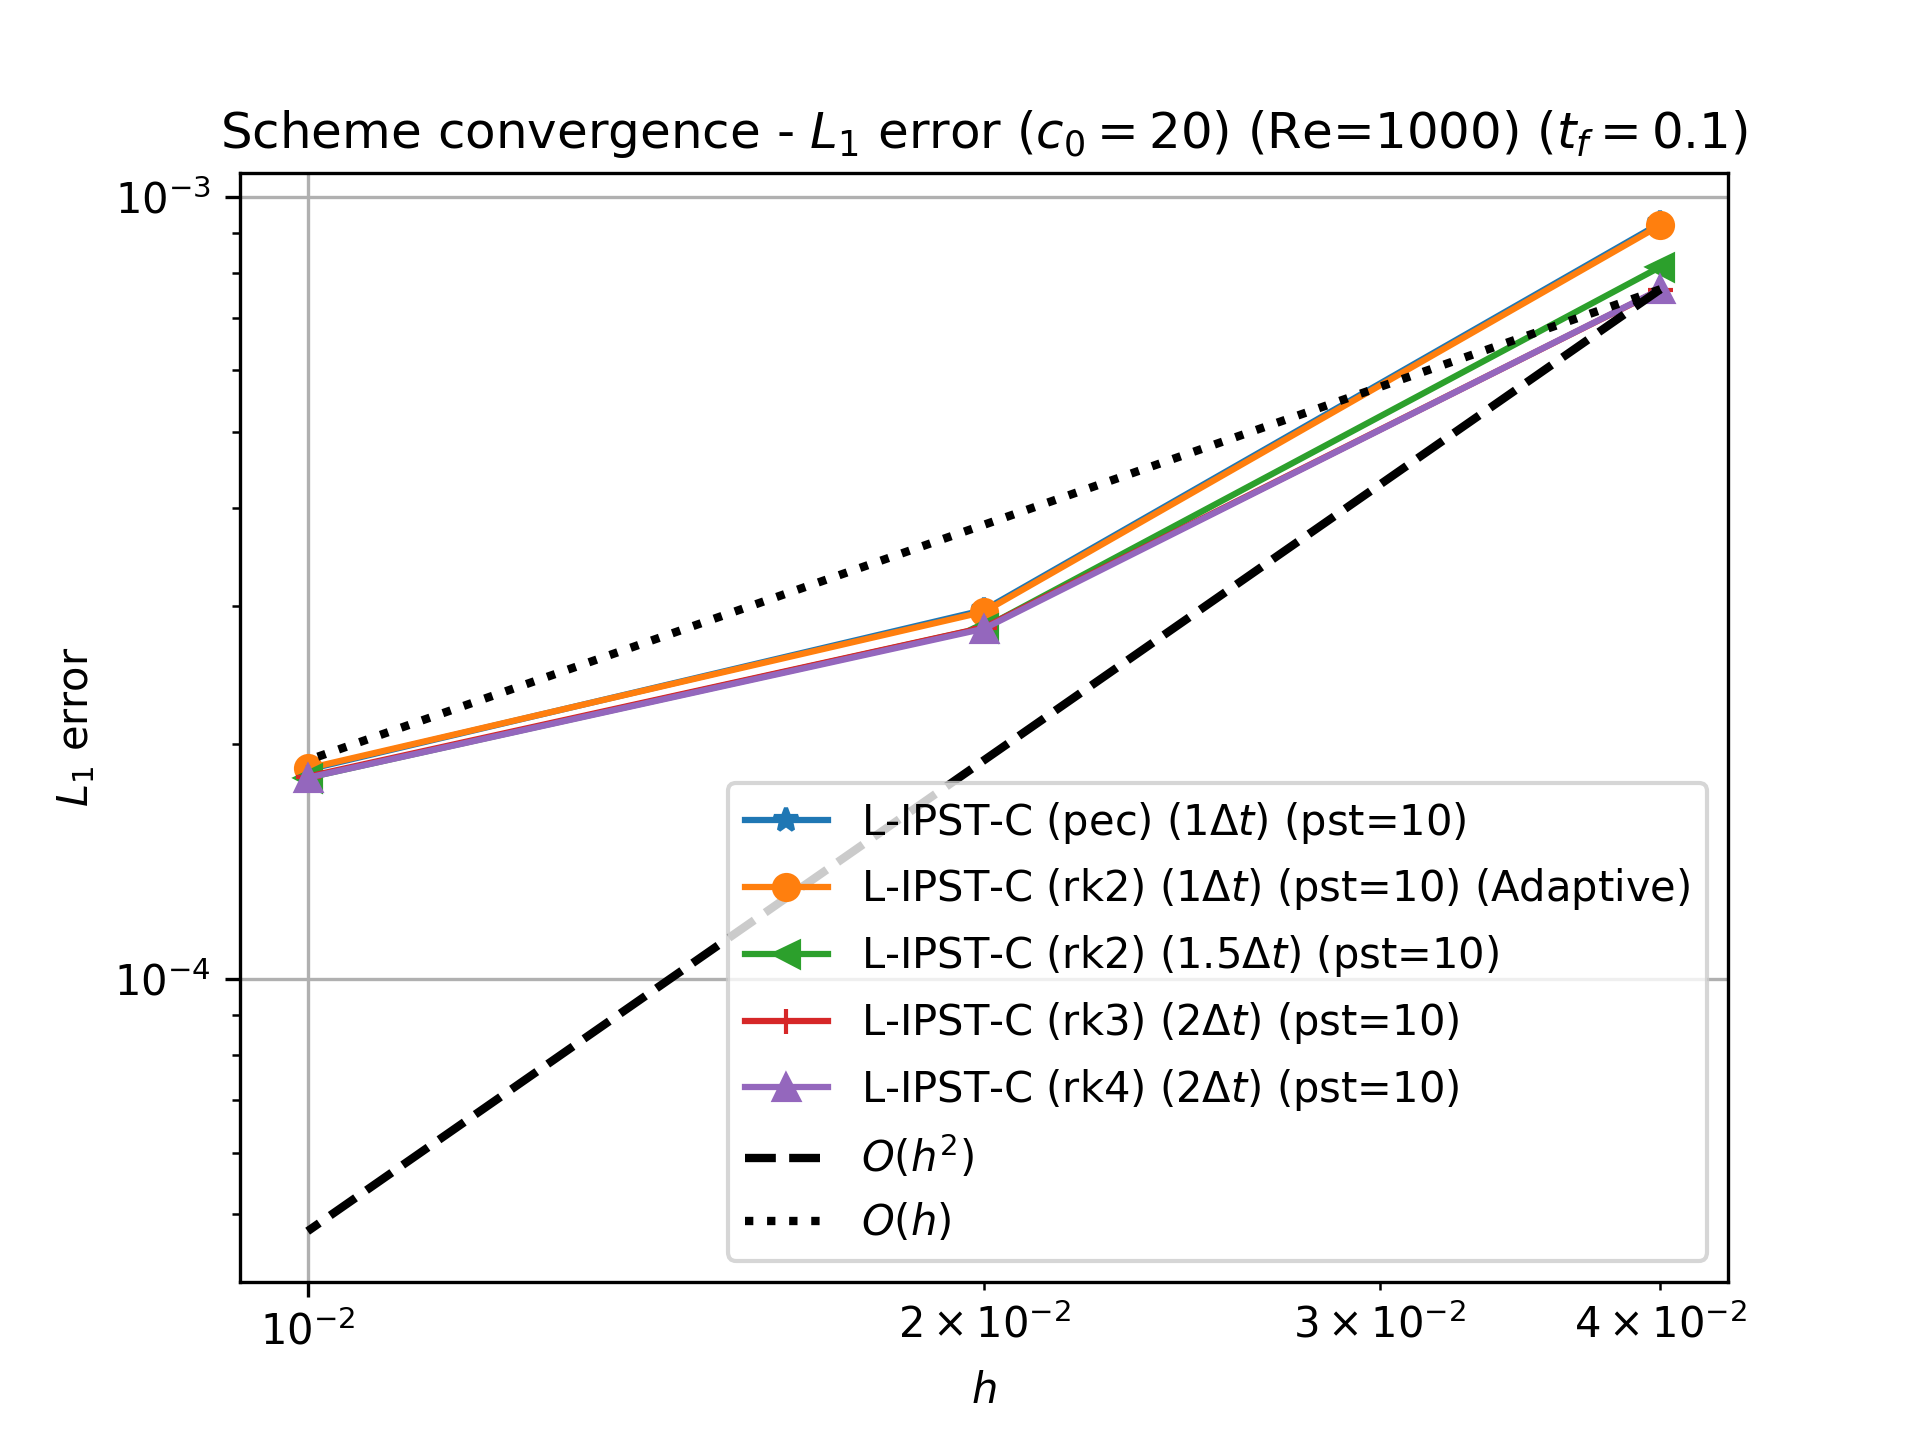
\includegraphics[width=6cm]{Code-Figures/lipstc/integrator/dt_pois_conv_c0_20_re_1000.png}
    \caption{$Re = 1000$}
  \end{subfigure}
  \begin{subfigure}{7cm}
    \centering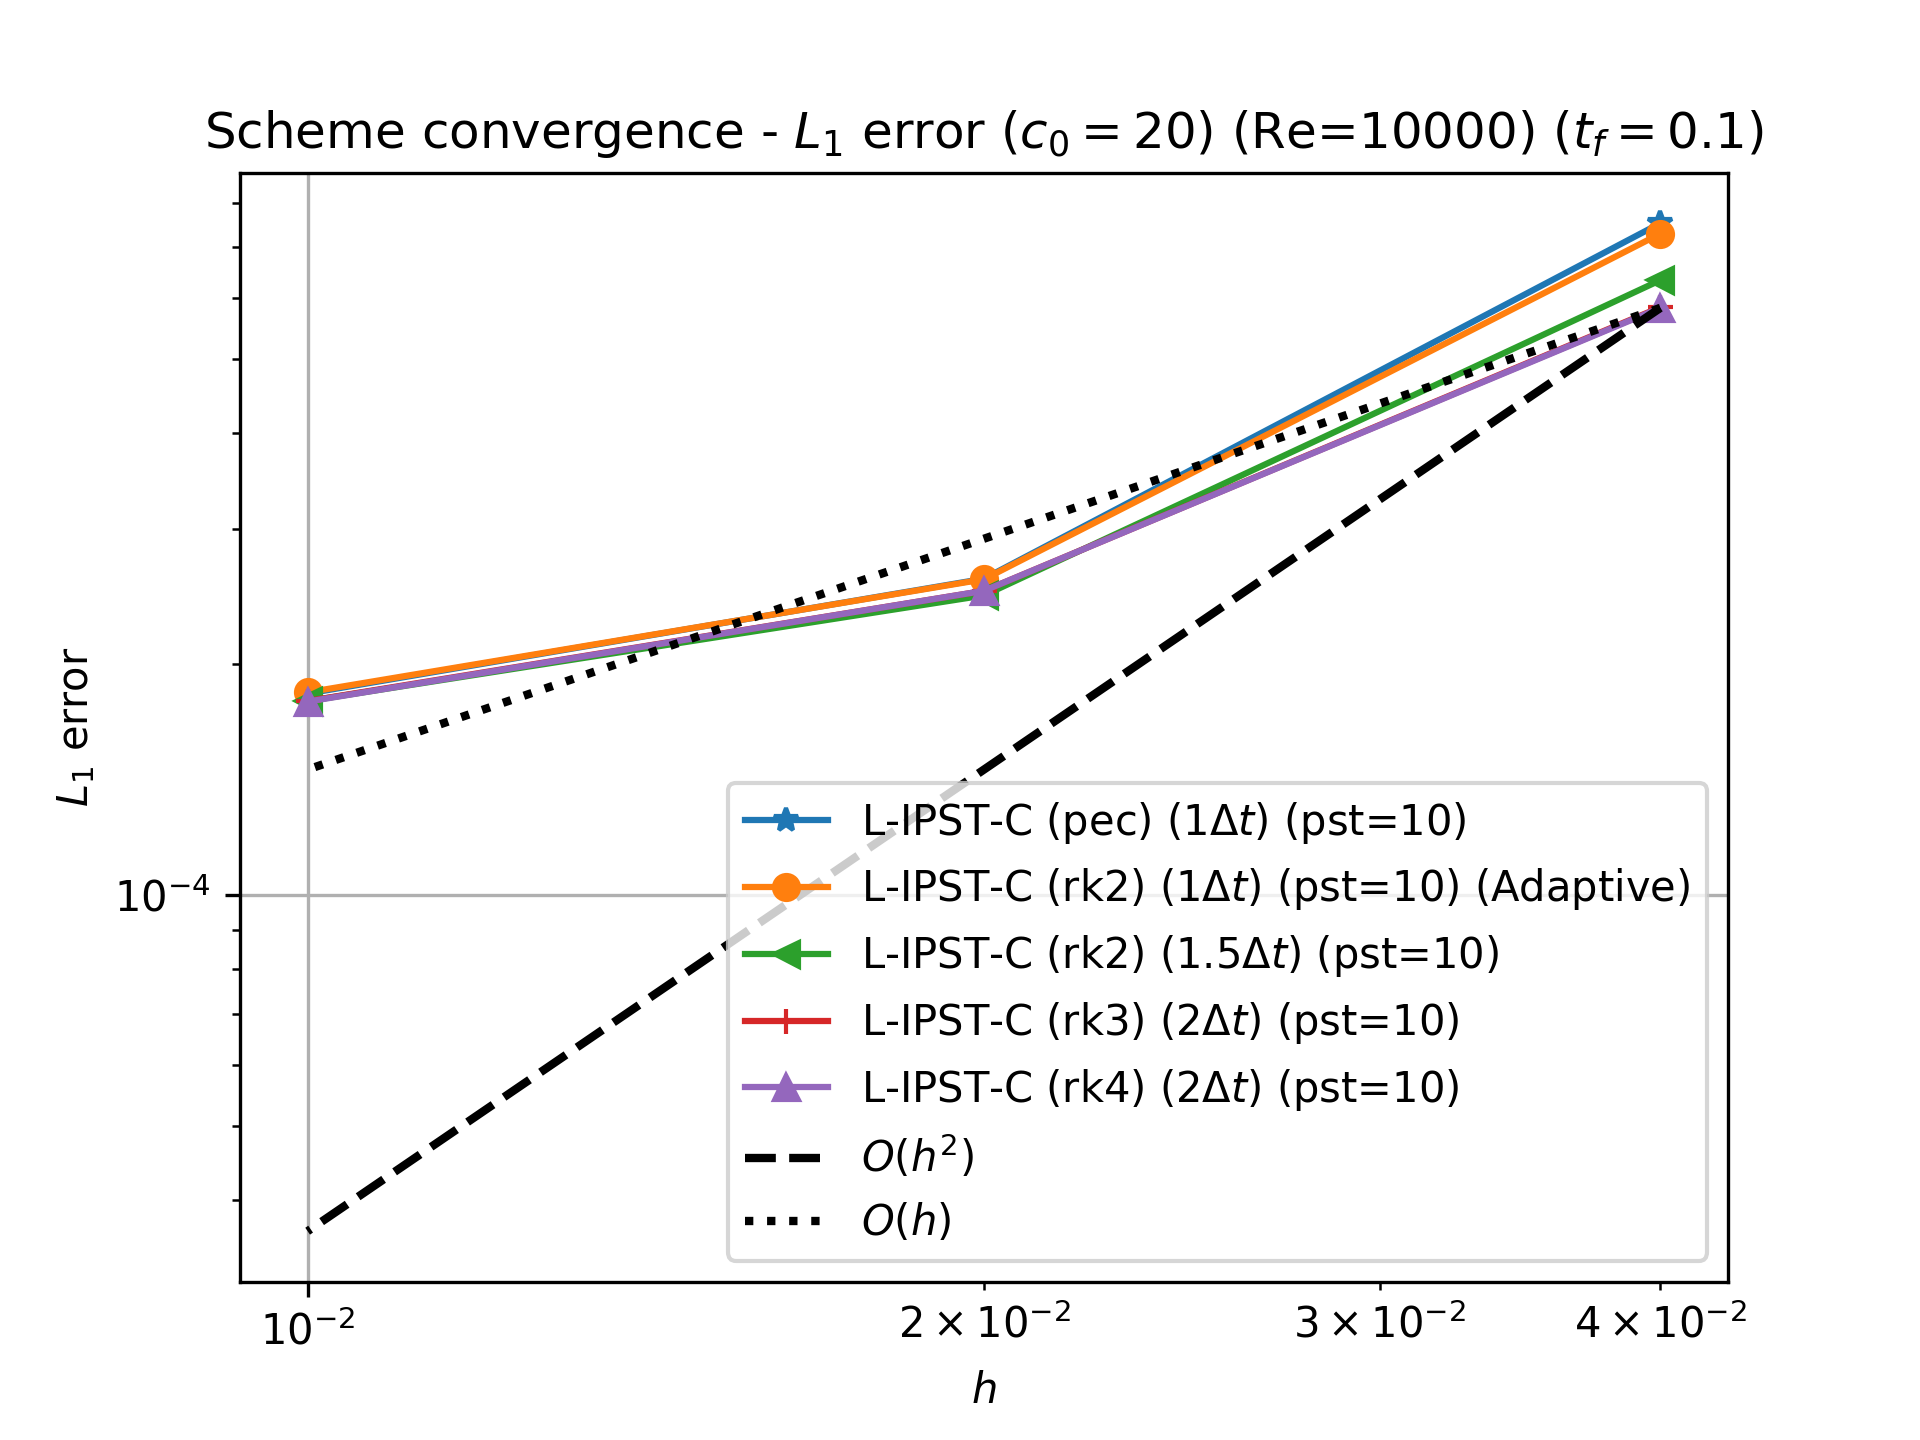
\includegraphics[width=6cm]{Code-Figures/lipstc/integrator/dt_pois_conv_c0_20_re_10000.png}
    \caption{$Re = 10000$}
  \end{subfigure}
  \caption{Convergence of the L-IPST-C scheme for various time-integration schemes.}
  \label{fig:lipstc-integrator}
\end{figure}

From the results shown in \figref{fig:lipstc-integrator}, it is evident that the order of the integrator does not appear to have much effect on the OOC, and almost negligible effect on the actual magnitude of the $L_1$ errors as well.
This seems to highlight a much more important aspect of the effect and role of time-integration schemes in SPH in general, which is that the time-step size is the most important factor, and the order of the integrator is not as important, since the time-step size is typically chosen to be small enough to ensure stability, and hence, the error introduced by the time-integration scheme is typically negligible.

Also, when the run-times of these integrators were analysed, the higher order integrators are observed to be more computationally expensive, allowing for the \texttt{PEC} integrator to be around $\approx 1.6\times$ faster, which is reflected in the run-times shown in \figref{fig:lipstc-integrator-rt}.
Typically such higher order integrators can be used with much larger $CFL$ values, allowing for larger time-steps and consequently faster run-times. However, in the case of SPH, such generalisations cannot be made, since the stability of the scheme is not only dependent on the time-step size, but also on the particle spacing, and hence, the $CFL$ value is typically chosen to be close to $1.0-2.0$.
Therefore, the \texttt{PEC} integrator is chosen as the default integrator for the L-IPST-C scheme.

\begin{figure}[H]
  \begin{subfigure}{7cm}
    \centering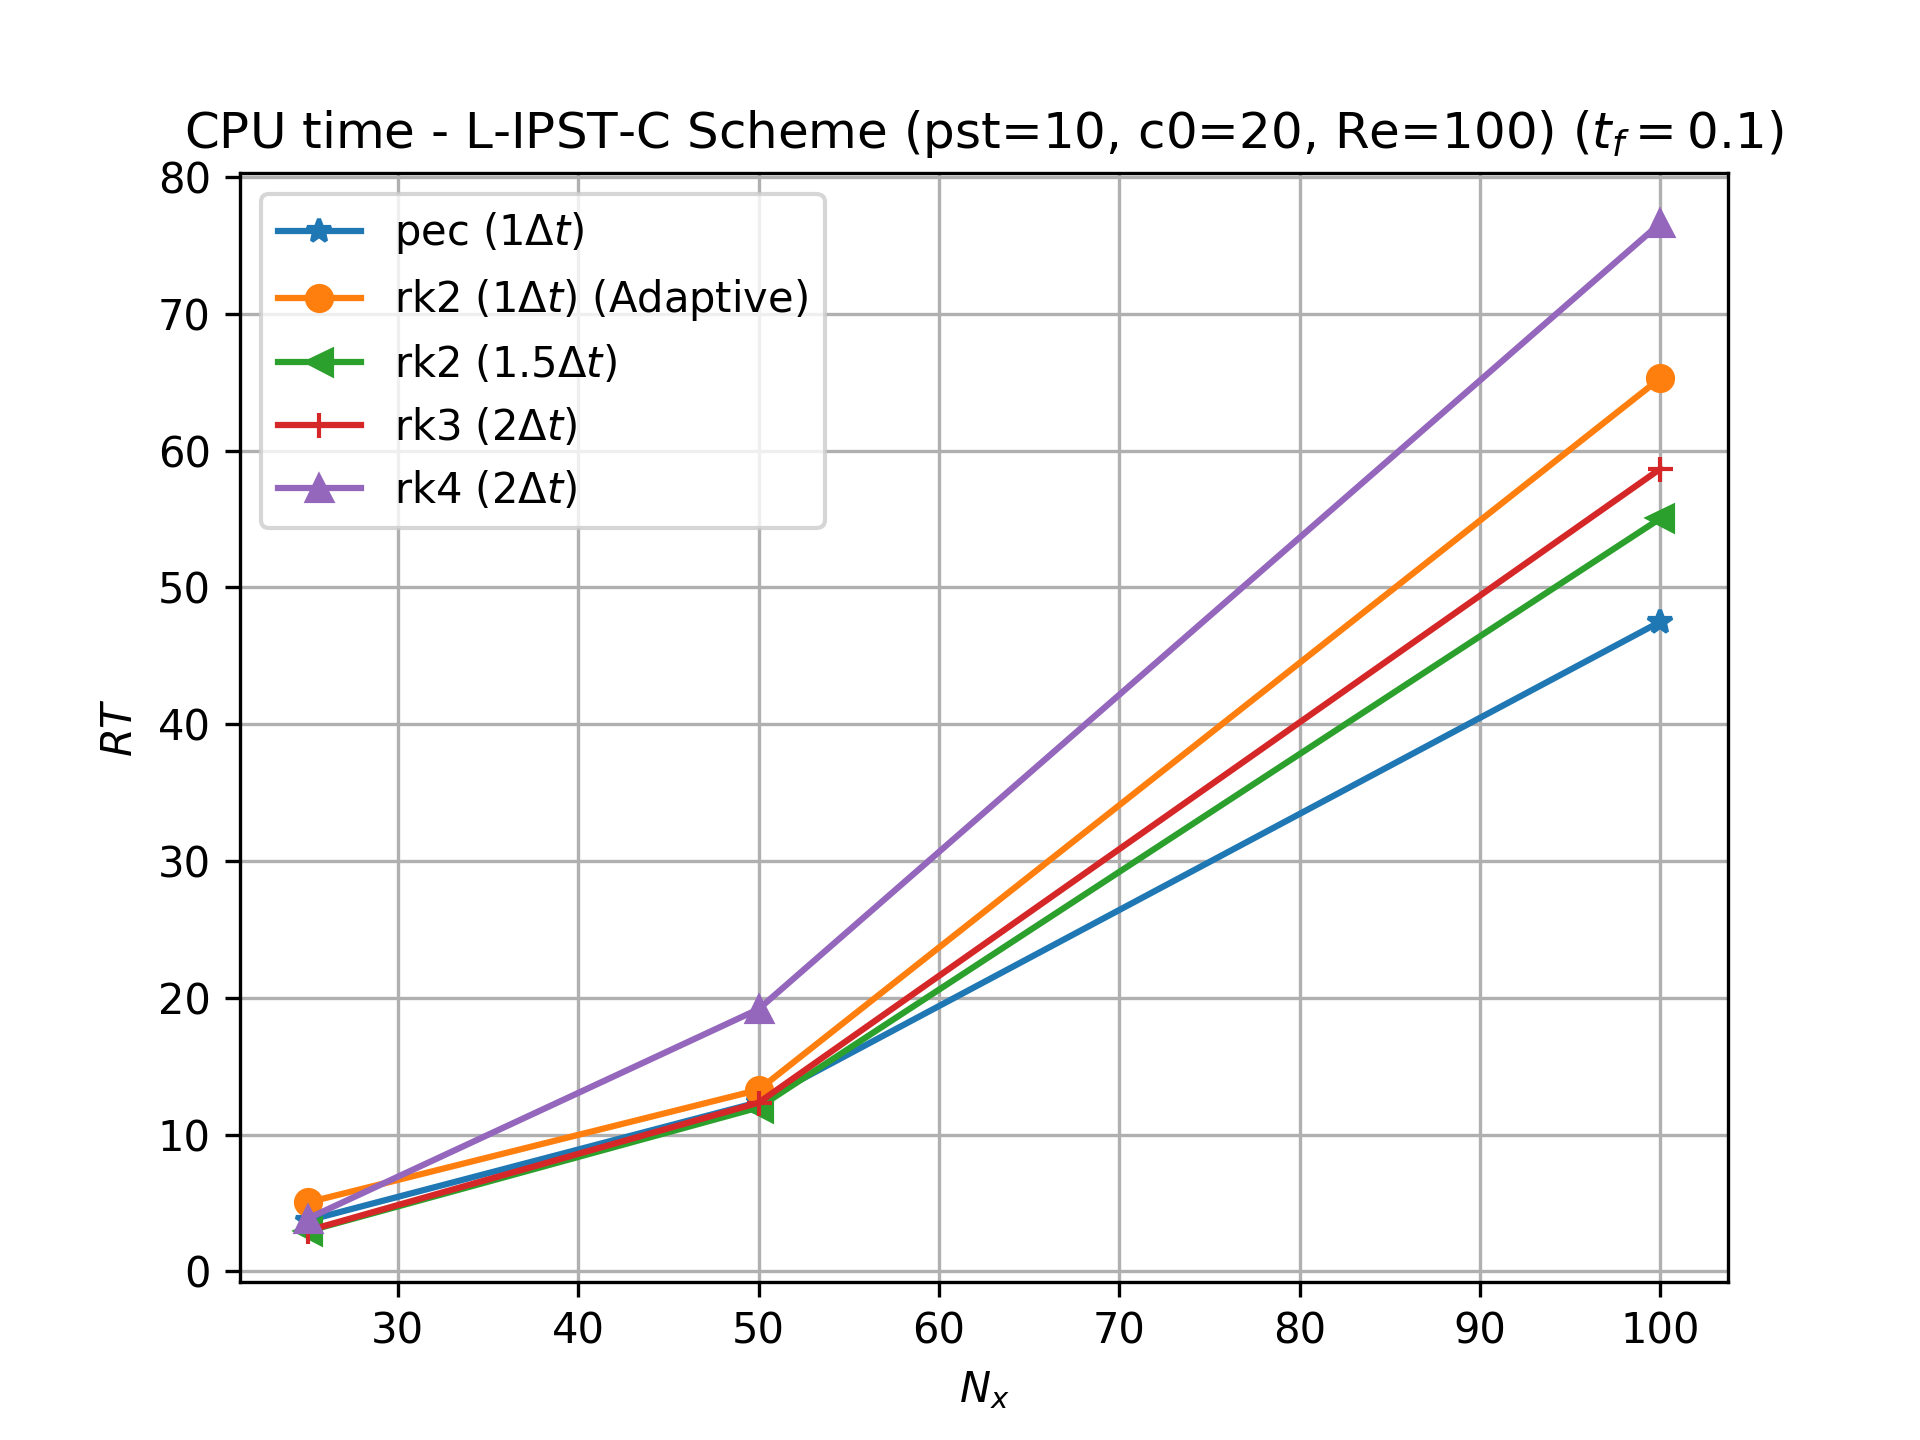
\includegraphics[width=6cm]{Code-Figures/lipstc/integrator/pois_rt_pst_10_c0_20_re_100.png}
    \caption{$Re = 100$}
  \end{subfigure}
  \begin{subfigure}{7cm}
    \centering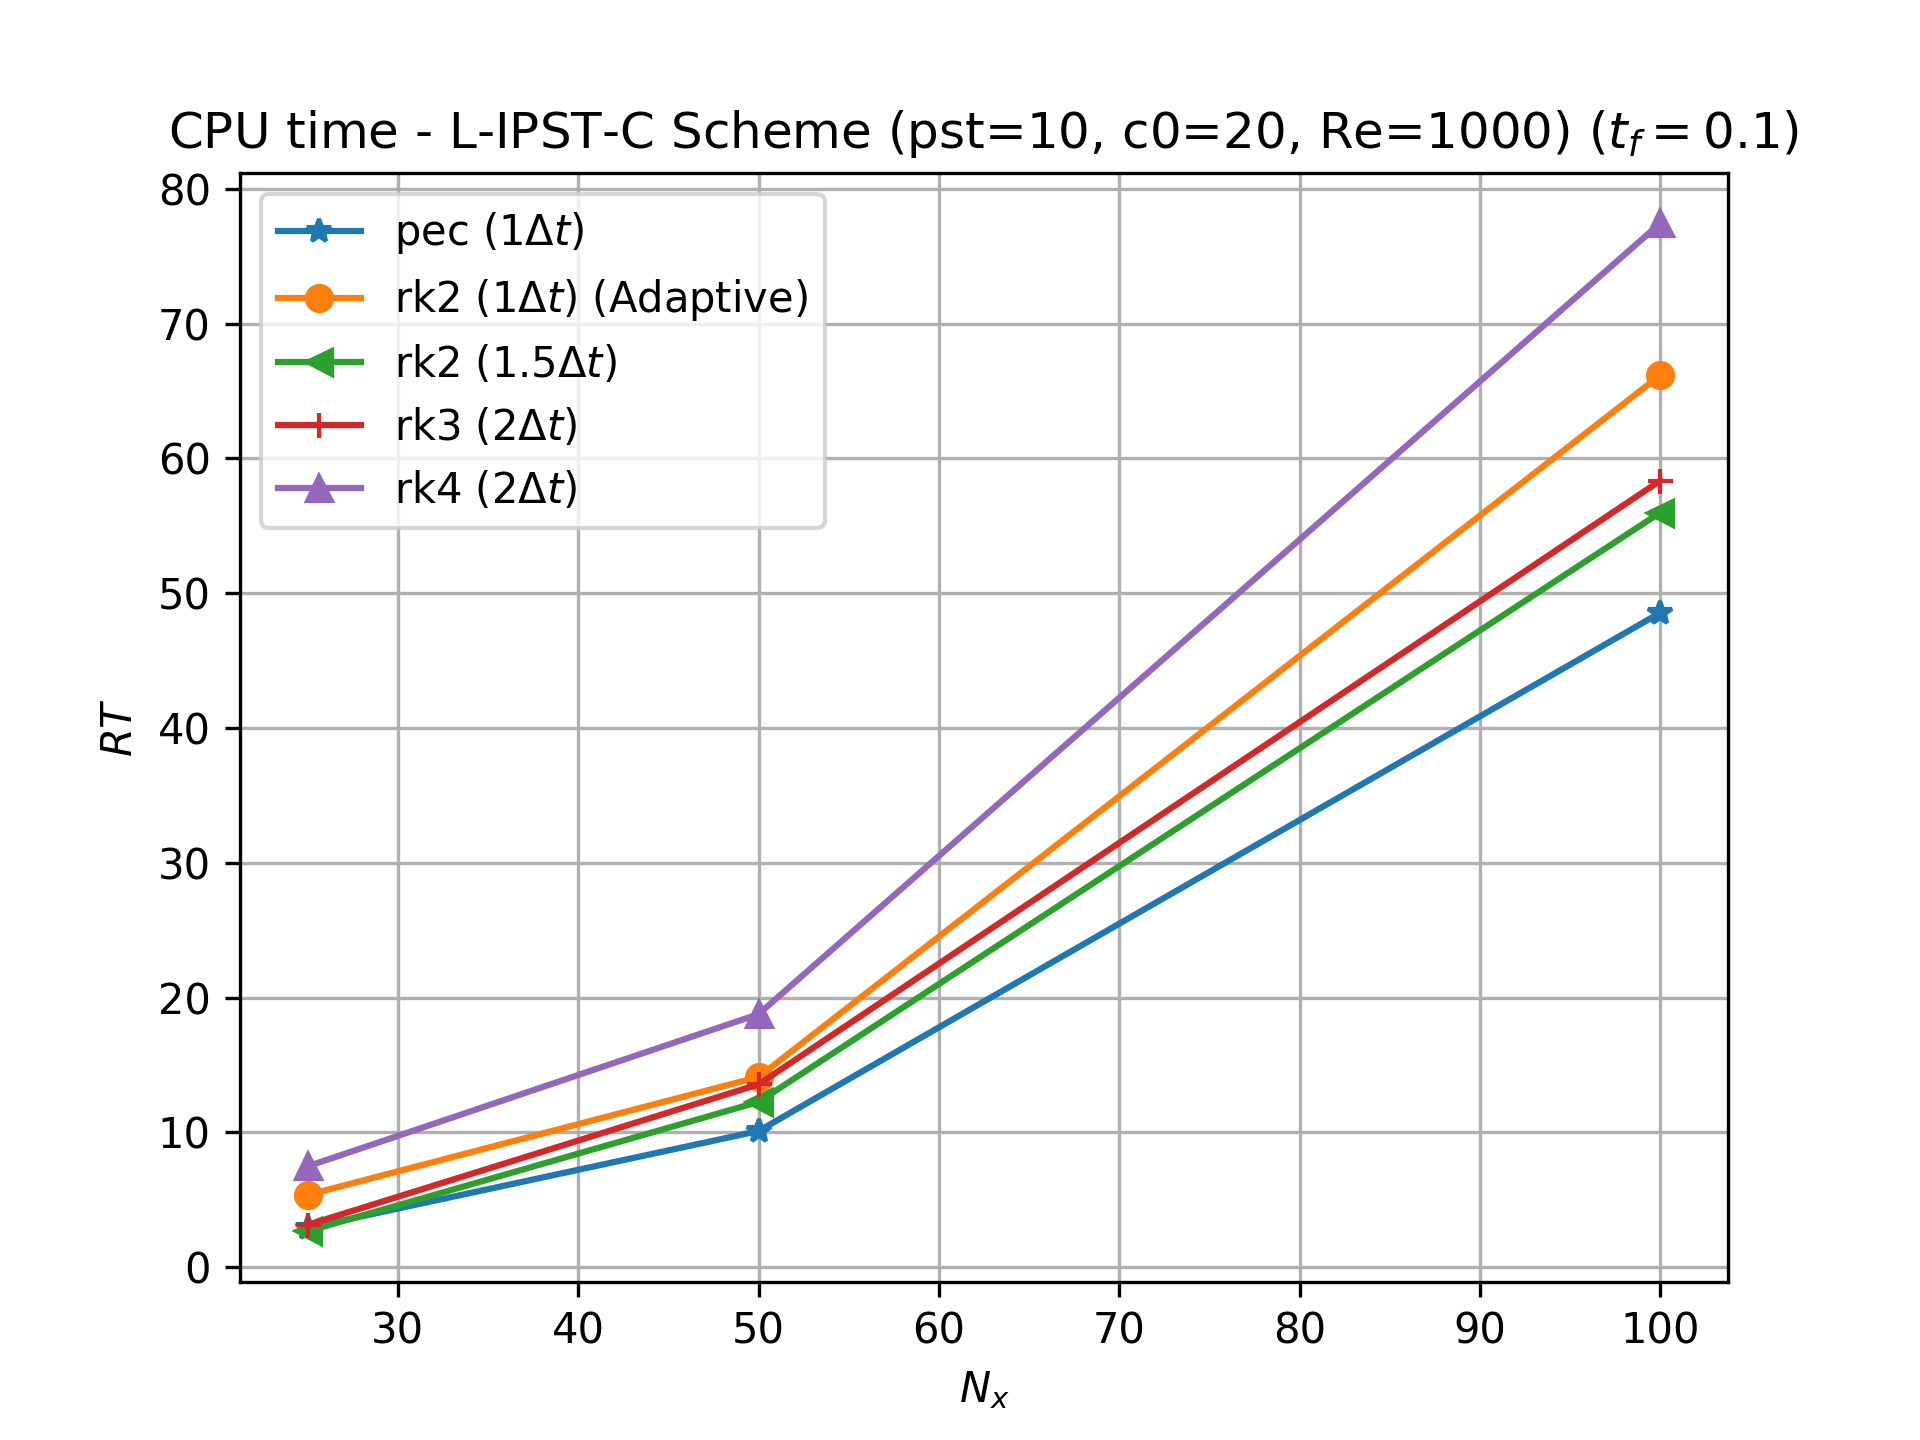
\includegraphics[width=6cm]{Code-Figures/lipstc/integrator/pois_rt_pst_10_c0_20_re_1000.png}
    \caption{$Re = 1000$}
  \end{subfigure}
  \begin{subfigure}{7cm}
    \centering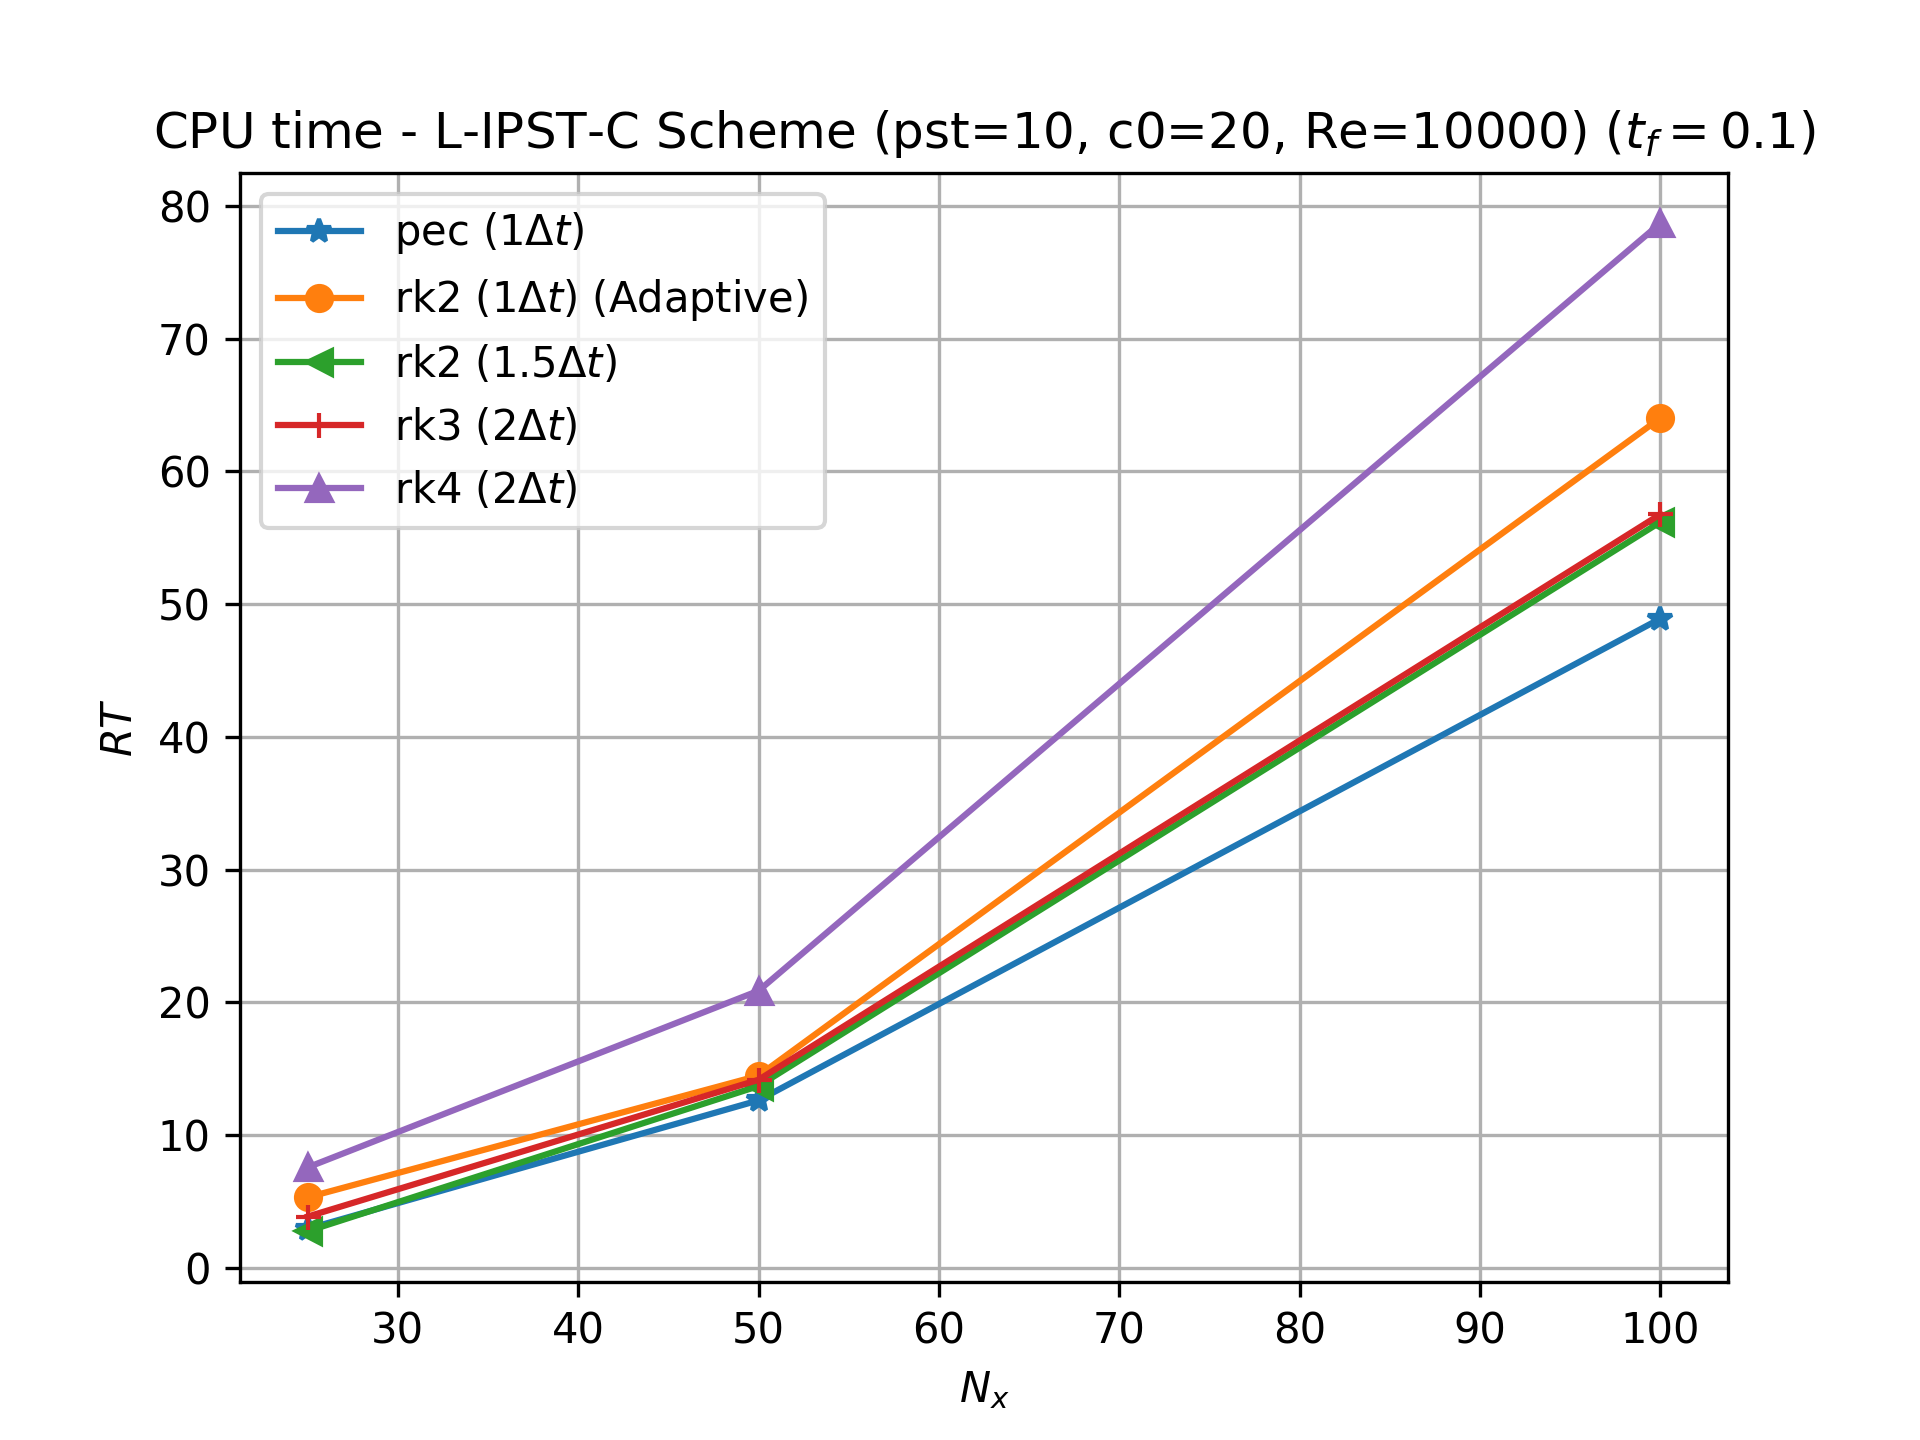
\includegraphics[width=6cm]{Code-Figures/lipstc/integrator/pois_rt_pst_10_c0_20_re_10000.png}
    \caption{$Re = 10000$}
  \end{subfigure}
  \caption{Run-time (in $s$) of the L-IPST-C scheme for various time-integration schemes.}
  \label{fig:lipstc-integrator-rt}
\end{figure}


\subsection{SPH-LES Scheme}
The SPH-LES scheme was considered over the other LES-based schemes, since the scheme utilised the compressible NS equations which were treated with a spatial averageing operator to obtain the filtered governing equations. They also considered, three different models for the turbulent eddy viscosity, which included the standard Smagorinsky model, $\sigma$-model and the standard model discretised in the Monaghan-Cleary-Gingold (MCG) form (detailed in \secref{sec:Modified-Smagorinsky-Model}). Therefore, the model appeared comprehensive in terms of its implementation, and hence, was chosen, along with the \texttt{SMAG} model, which is the standard Smagorinsky model, since their study revealed that this model was the most accurate relatively in terms of its prediction of the energy spectrum, while using the \texttt{PEC} integrator.

\begin{figure}[H]
  \begin{subfigure}{7cm}
    \centering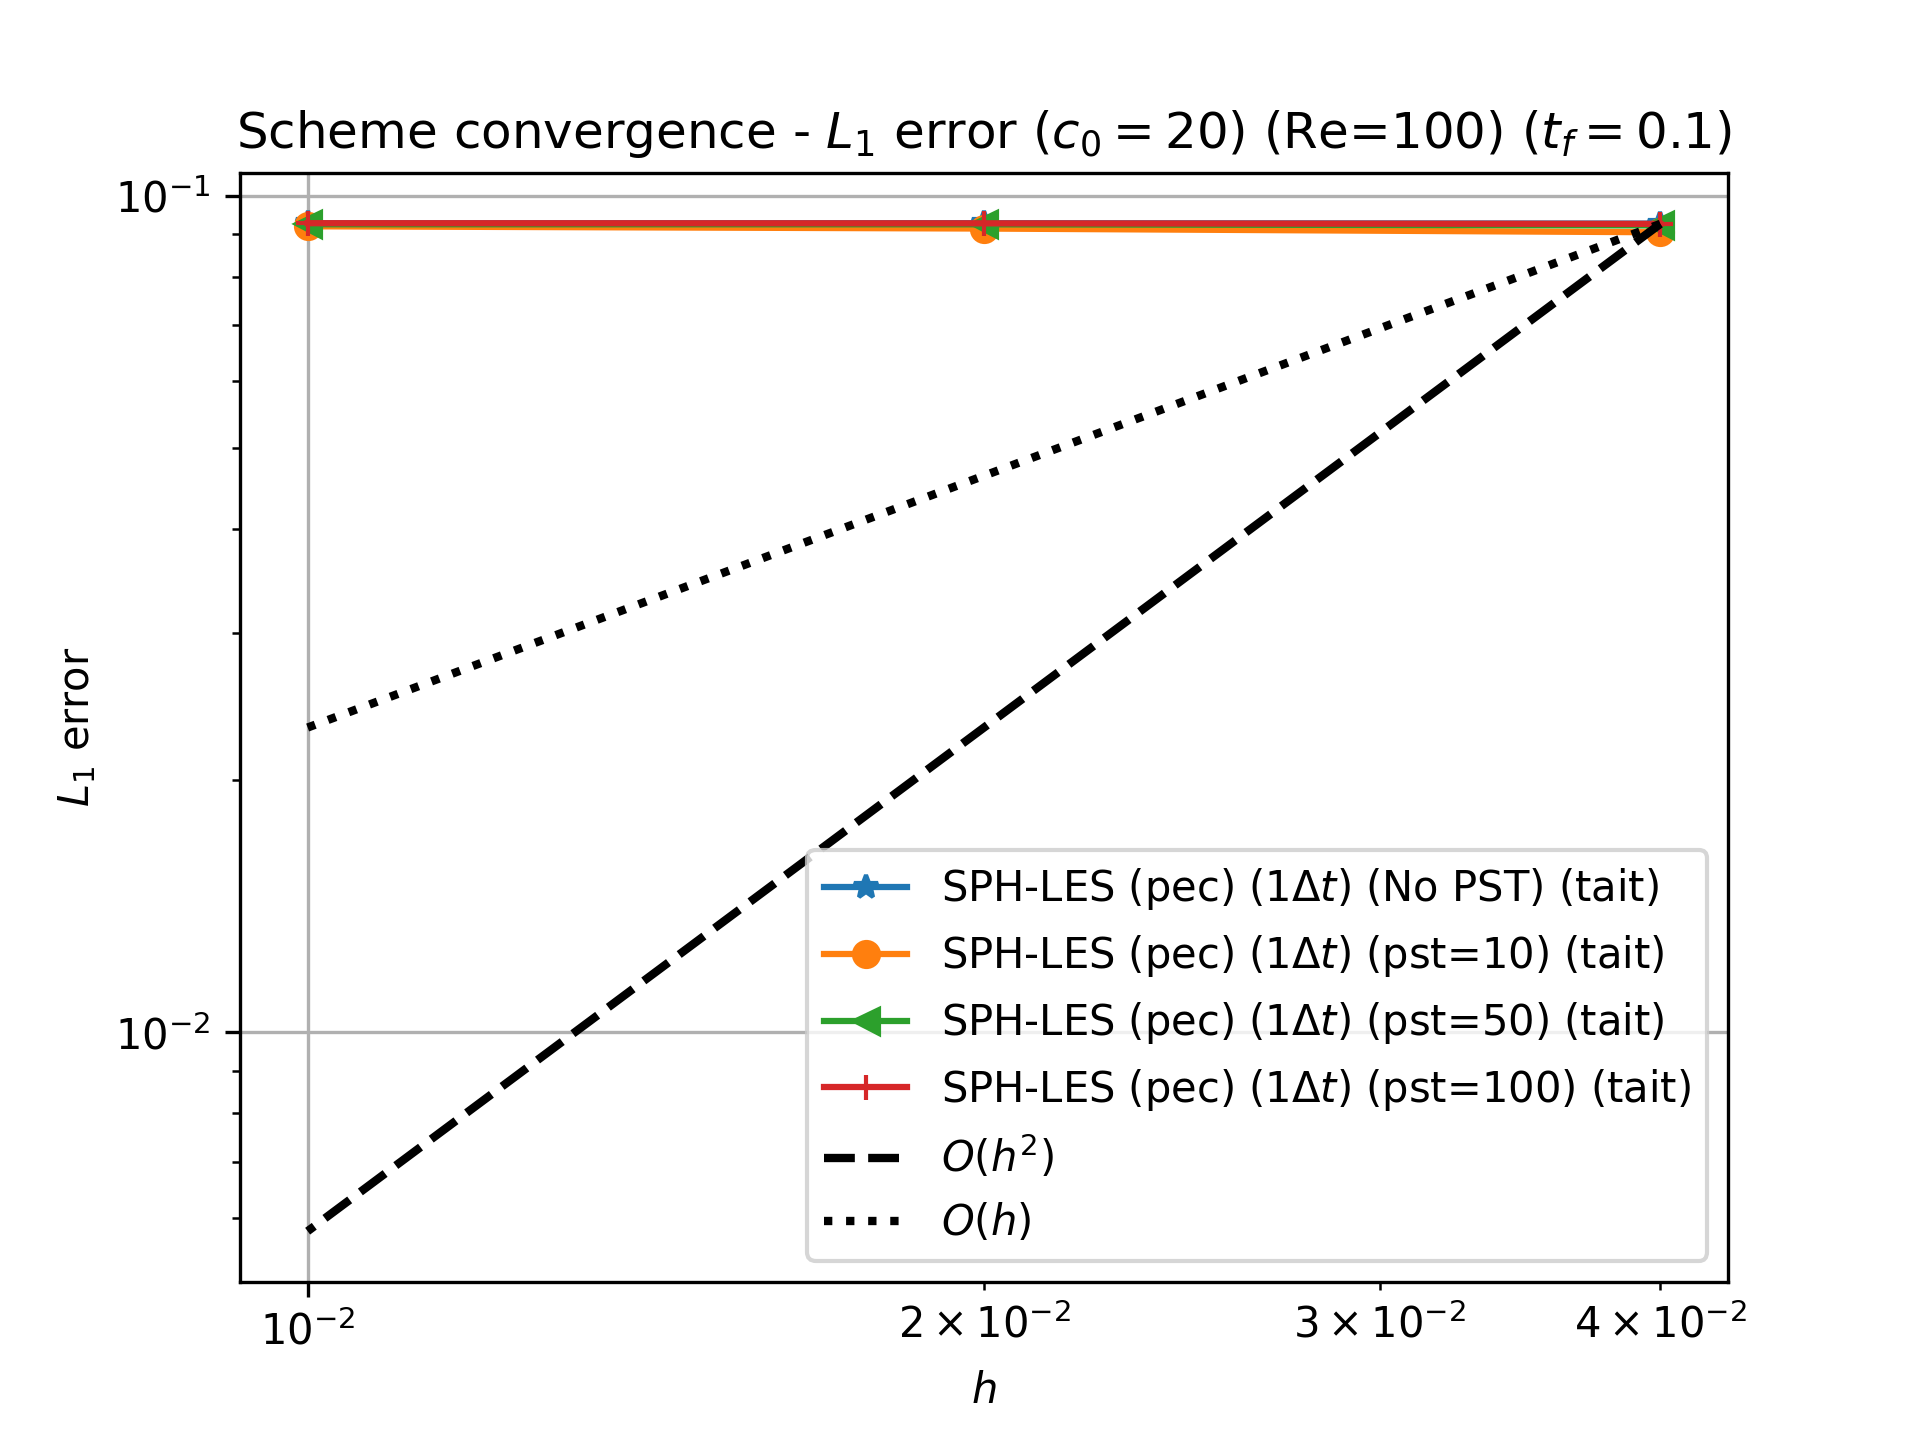
\includegraphics[width=6cm]{Code-Figures/okra2022/pst/dt_pois_conv_c0_20_re_100.png}
    \caption{$Re = 100$}
  \end{subfigure}
  \begin{subfigure}{7cm}
    \centering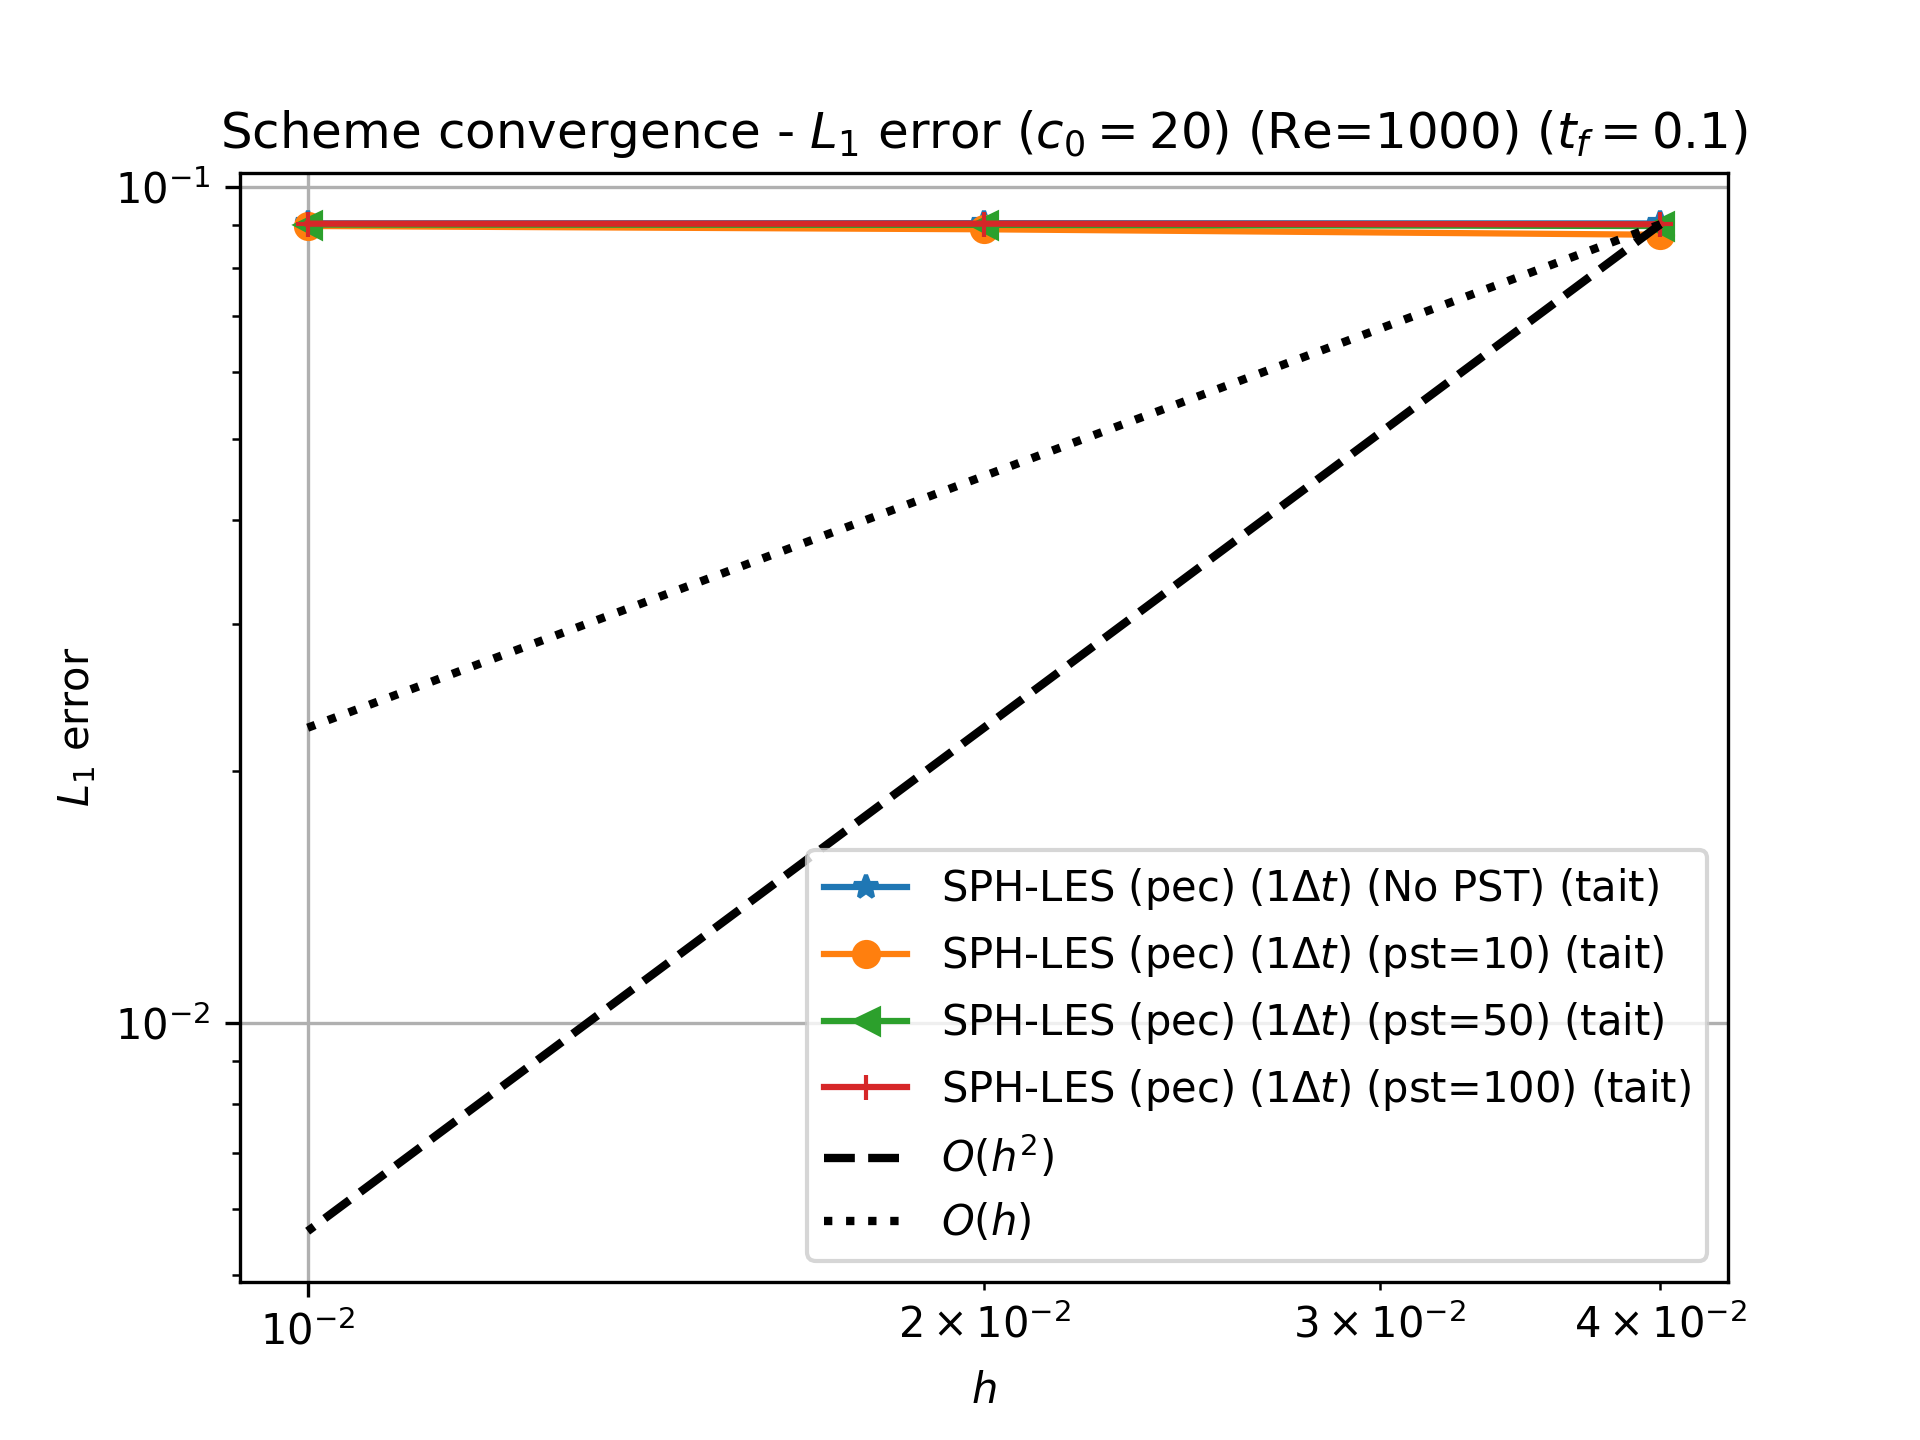
\includegraphics[width=6cm]{Code-Figures/okra2022/pst/dt_pois_conv_c0_20_re_1000.png}
    \caption{$Re = 1000$}
  \end{subfigure}
  \begin{subfigure}{7cm}
    \centering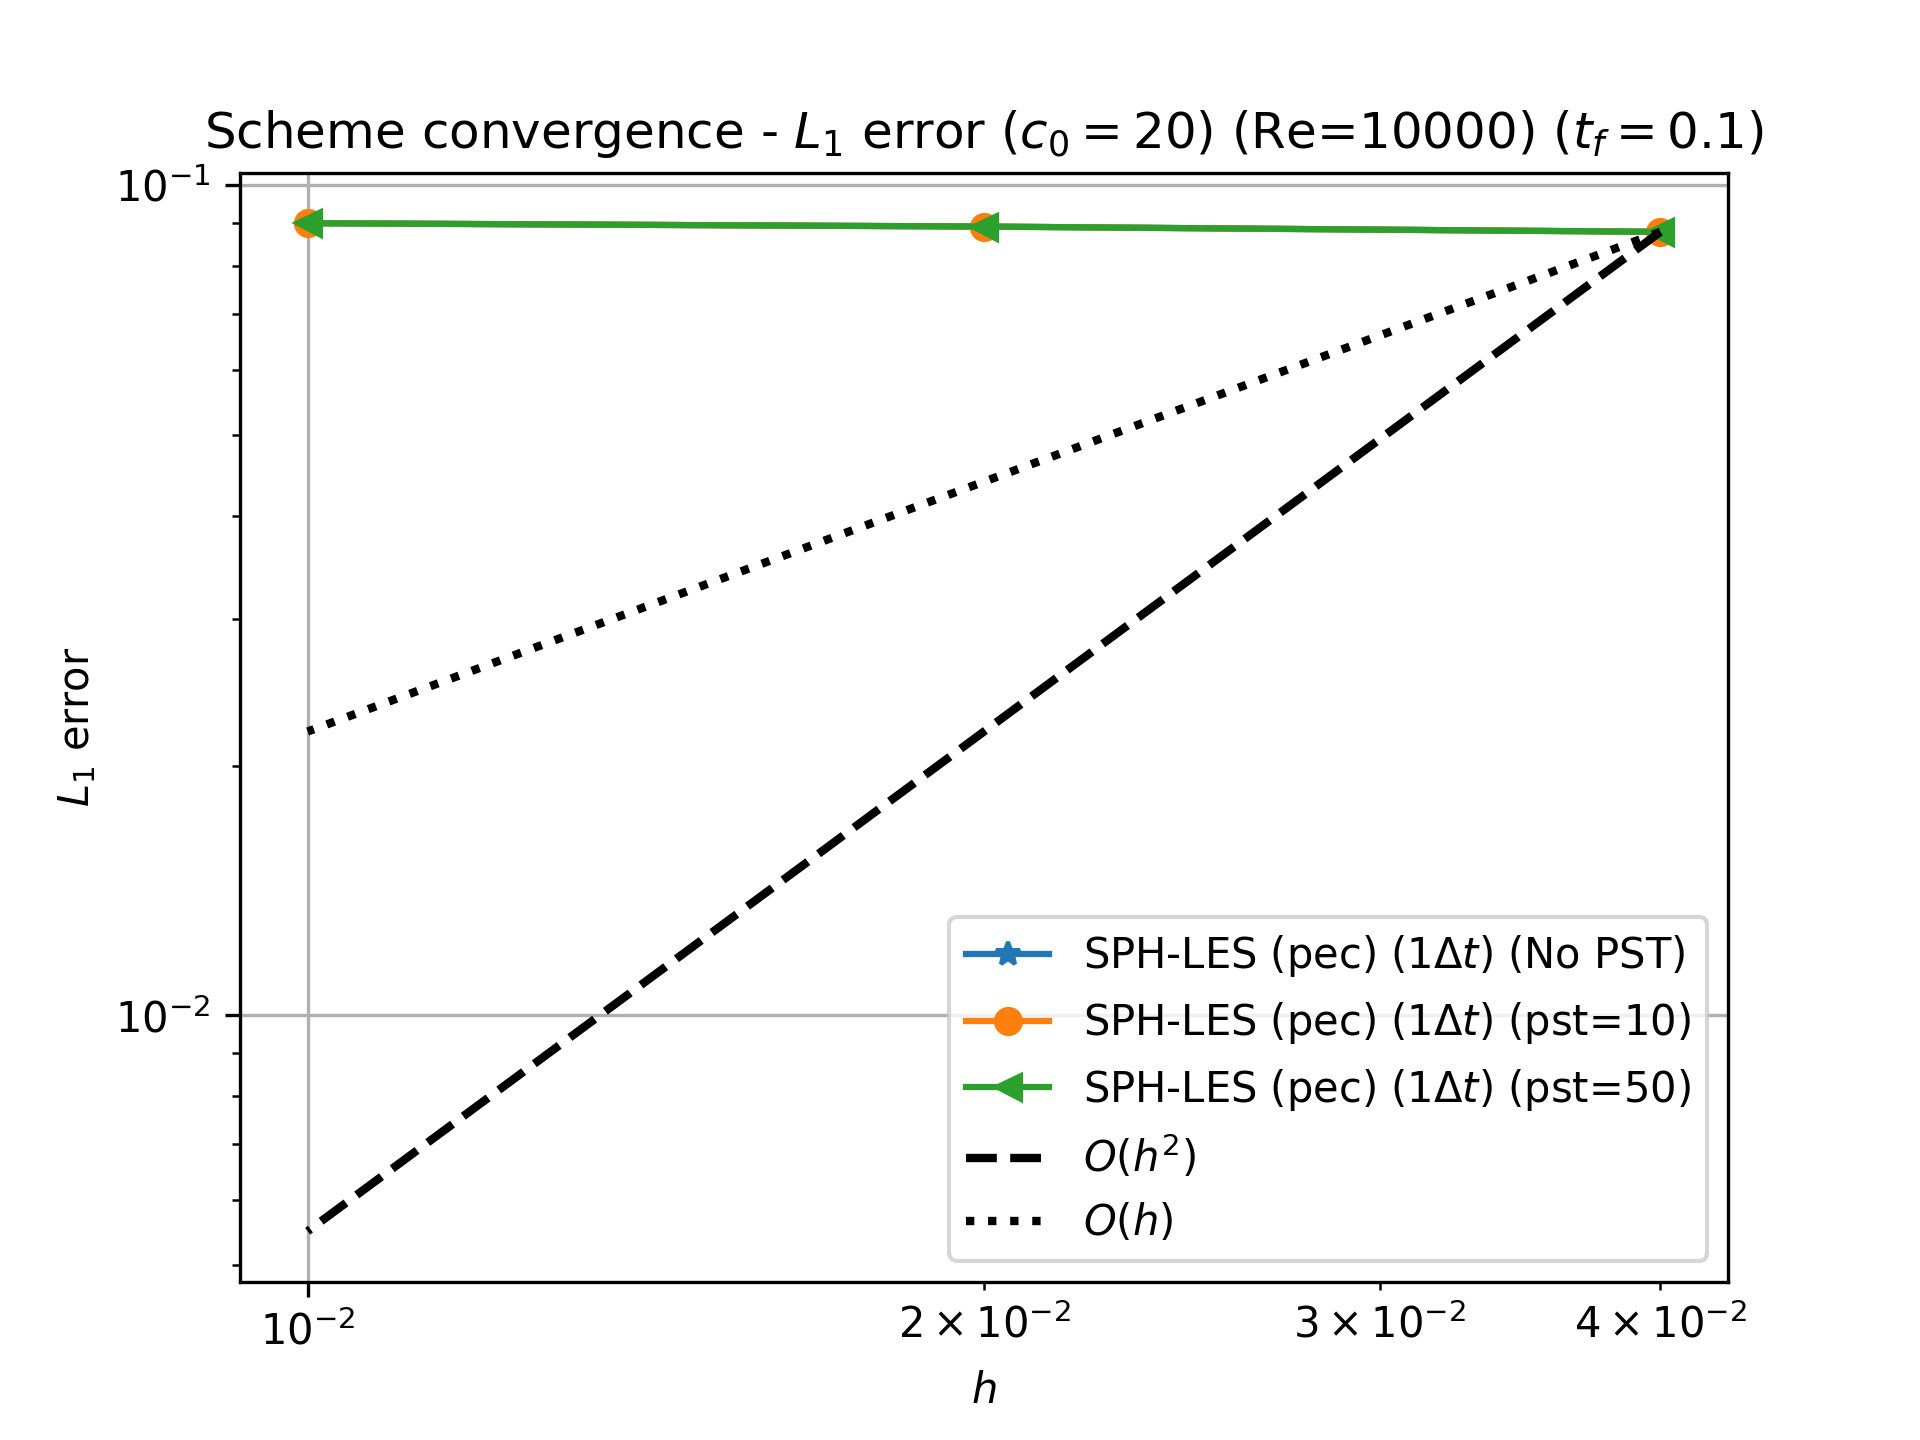
\includegraphics[width=6cm]{Code-Figures/okra2022/pst/dt_pois_conv_c0_20_re_10000.png}
    \caption{$Re = 10000$}
  \end{subfigure}
  \caption{Convergence of the SPH-LES scheme for various $f_{pst}$ values.}
  \label{fig:okra2022-pst}
\end{figure}


In order to identify the effects of the PST on the scheme, the following values were considered: $f_{pst} = [None, 10, 50, 100]$, with the speed of sound for the particles through PST to be $c_s = 20$. The results are shown in \figref{fig:okra2022-pst}, where it can be seen that the scheme worringly appears to be zero order convergent. To gain a better understanding of the forces, the velocity magnitude field and the energy spectrum were plotted.
In \figref{fig:okra2022-pst-vmag}, it can be observed that without PST, the particles get clustered, and there are marked regions which are devoid of particles. It is also evident, that high values of $f_{PST}$ are also not desirable, since it leads to the particles being clustered in a different manner, and also leads to the formation of void regions.
Also, in \figref{fig:okra2022-pst-espec}, it can be observed that the slope of the energy spectrum at the final time instance (yellow line), increases with increasing values of $f_{pst}$, which is indicative of the fact that the energy is being concentrated at the higher resolution scales, which is expected for the high $Re$ case.
Therefore, a value of $f_{pst} = 10$ is chosen as the default value for the PST.

\begin{figure}[H]
  \begin{subfigure}{7cm}
    \centering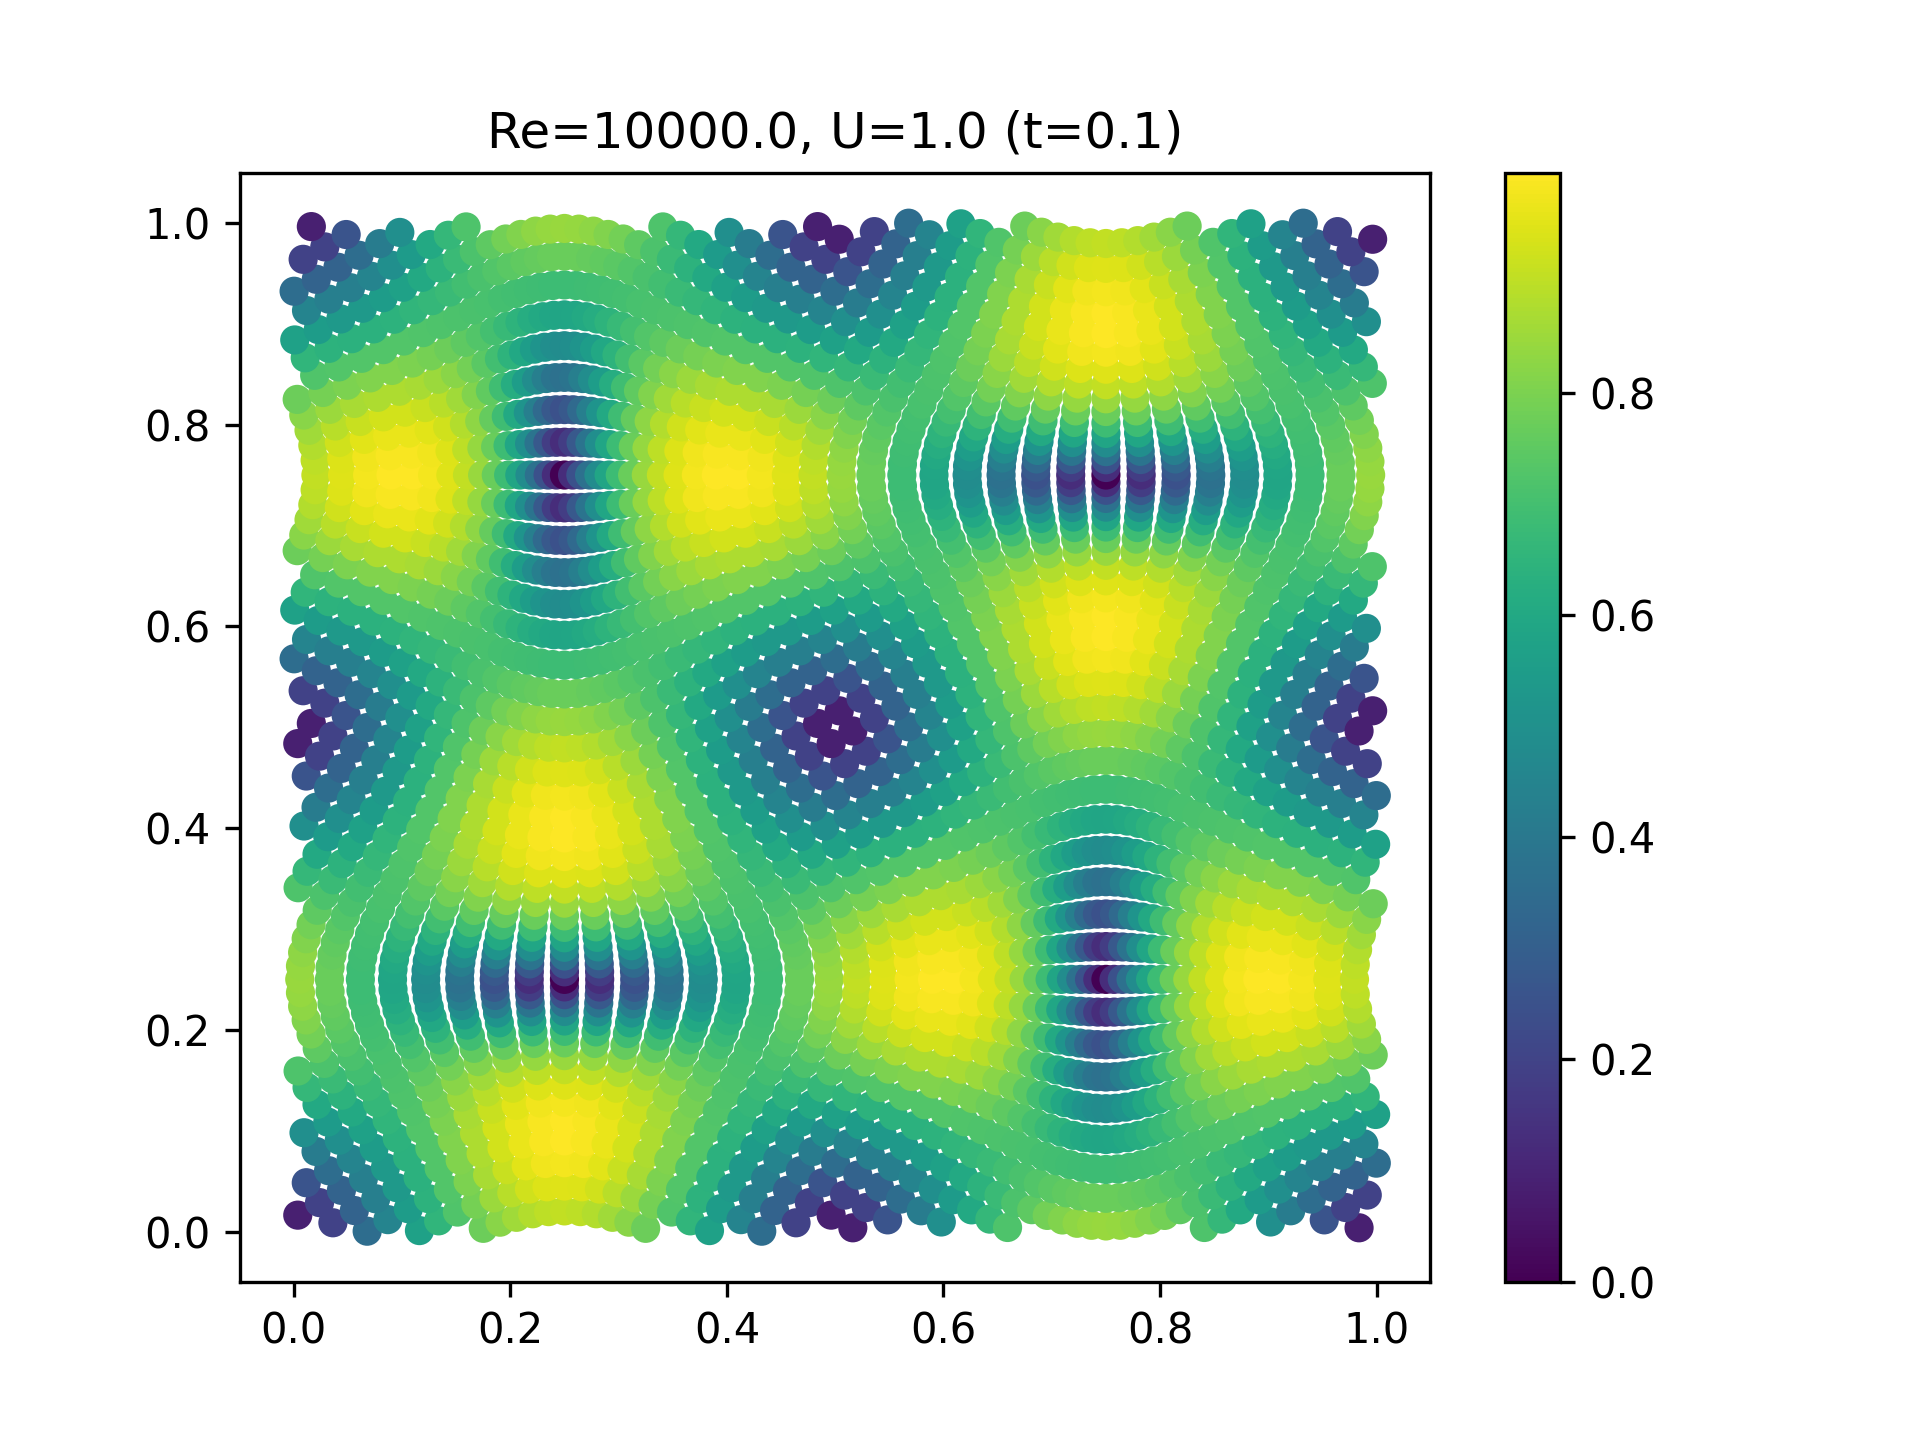
\includegraphics[width=6cm]{Code-Figures/okra2022/pst/c0_20_tait_pec_dtmul_1_nx_50_pst_-1_re_10000_ok2022/final_vmag.png}
    \caption{No PST}
  \end{subfigure}
  \begin{subfigure}{7cm}
    \centering\includegraphics[width=6cm]{Code-Figures/okra2022/pst/c0_20_tait_pec_dtmul_1_nx_50_pst_10_re_10000_ok2022/final_vmag.png}
    \caption{$f_{pst} = 10$}
  \end{subfigure}
  \begin{subfigure}{7cm}
    \centering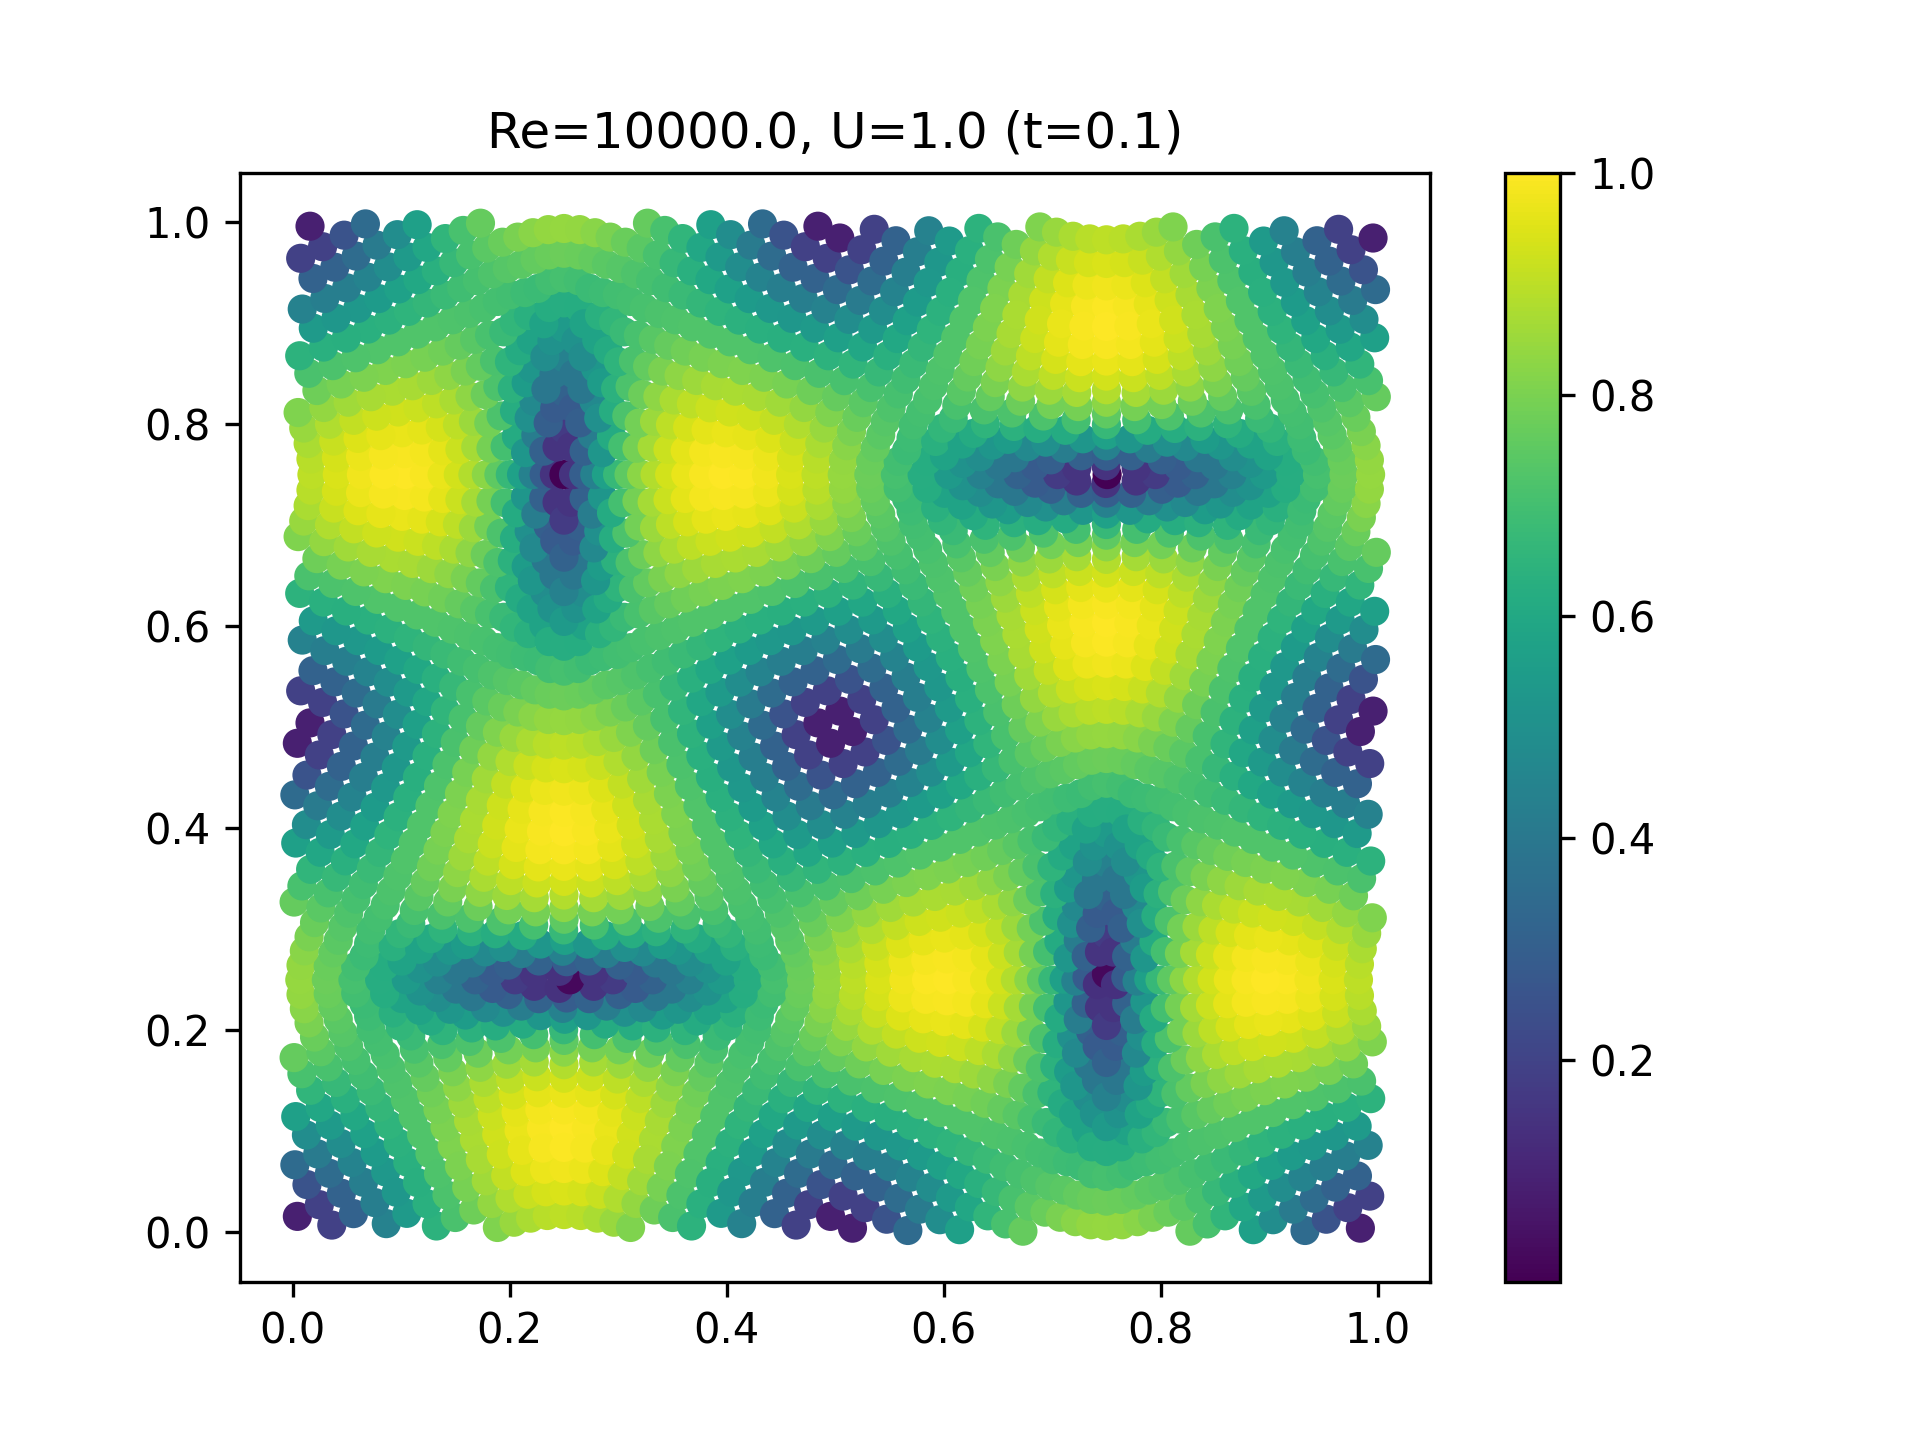
\includegraphics[width=6cm]{Code-Figures/okra2022/pst/c0_20_tait_pec_dtmul_1_nx_50_pst_50_re_10000_ok2022/final_vmag.png}
    \caption{$f_{pst} = 50$}
  \end{subfigure}
  \begin{subfigure}{7cm}
    \centering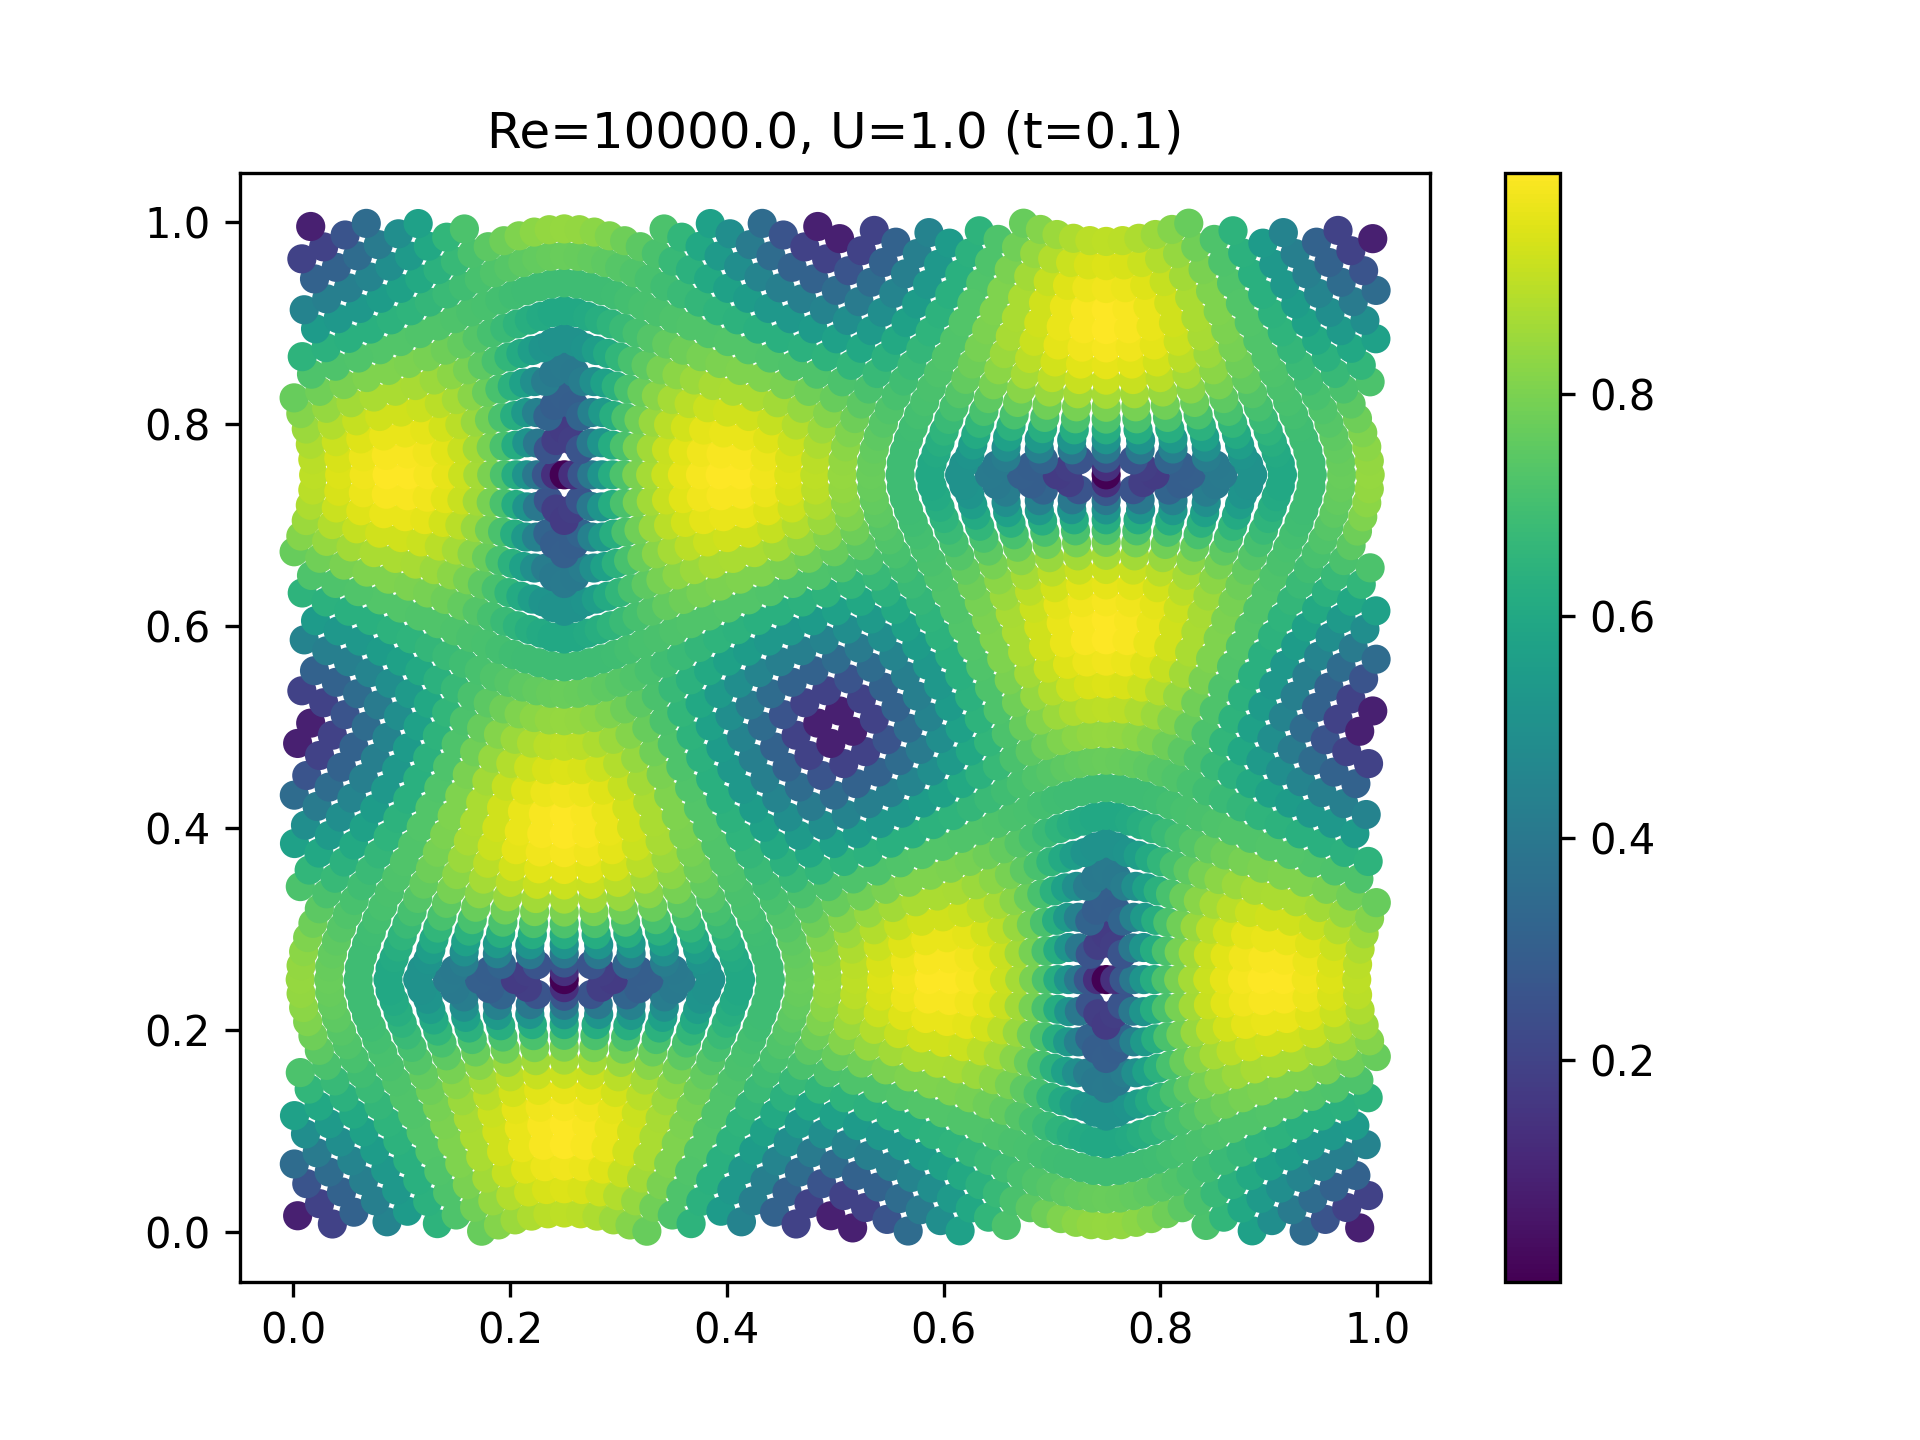
\includegraphics[width=6cm]{Code-Figures/okra2022/pst/c0_20_tait_pec_dtmul_1_nx_50_pst_100_re_10000_ok2022/final_vmag.png}
    \caption{$f_{pst} = 100$}
  \end{subfigure}
  \caption{Velocity magnitude field for the SPH-LES scheme for various $f_{pst}$ values $(N=50^2, t_f=0.1, Re=10000, c_s=20)$.}
  \label{fig:okra2022-pst-vmag}
\end{figure}

\begin{figure}[H]
  \begin{subfigure}{7cm}
    \centering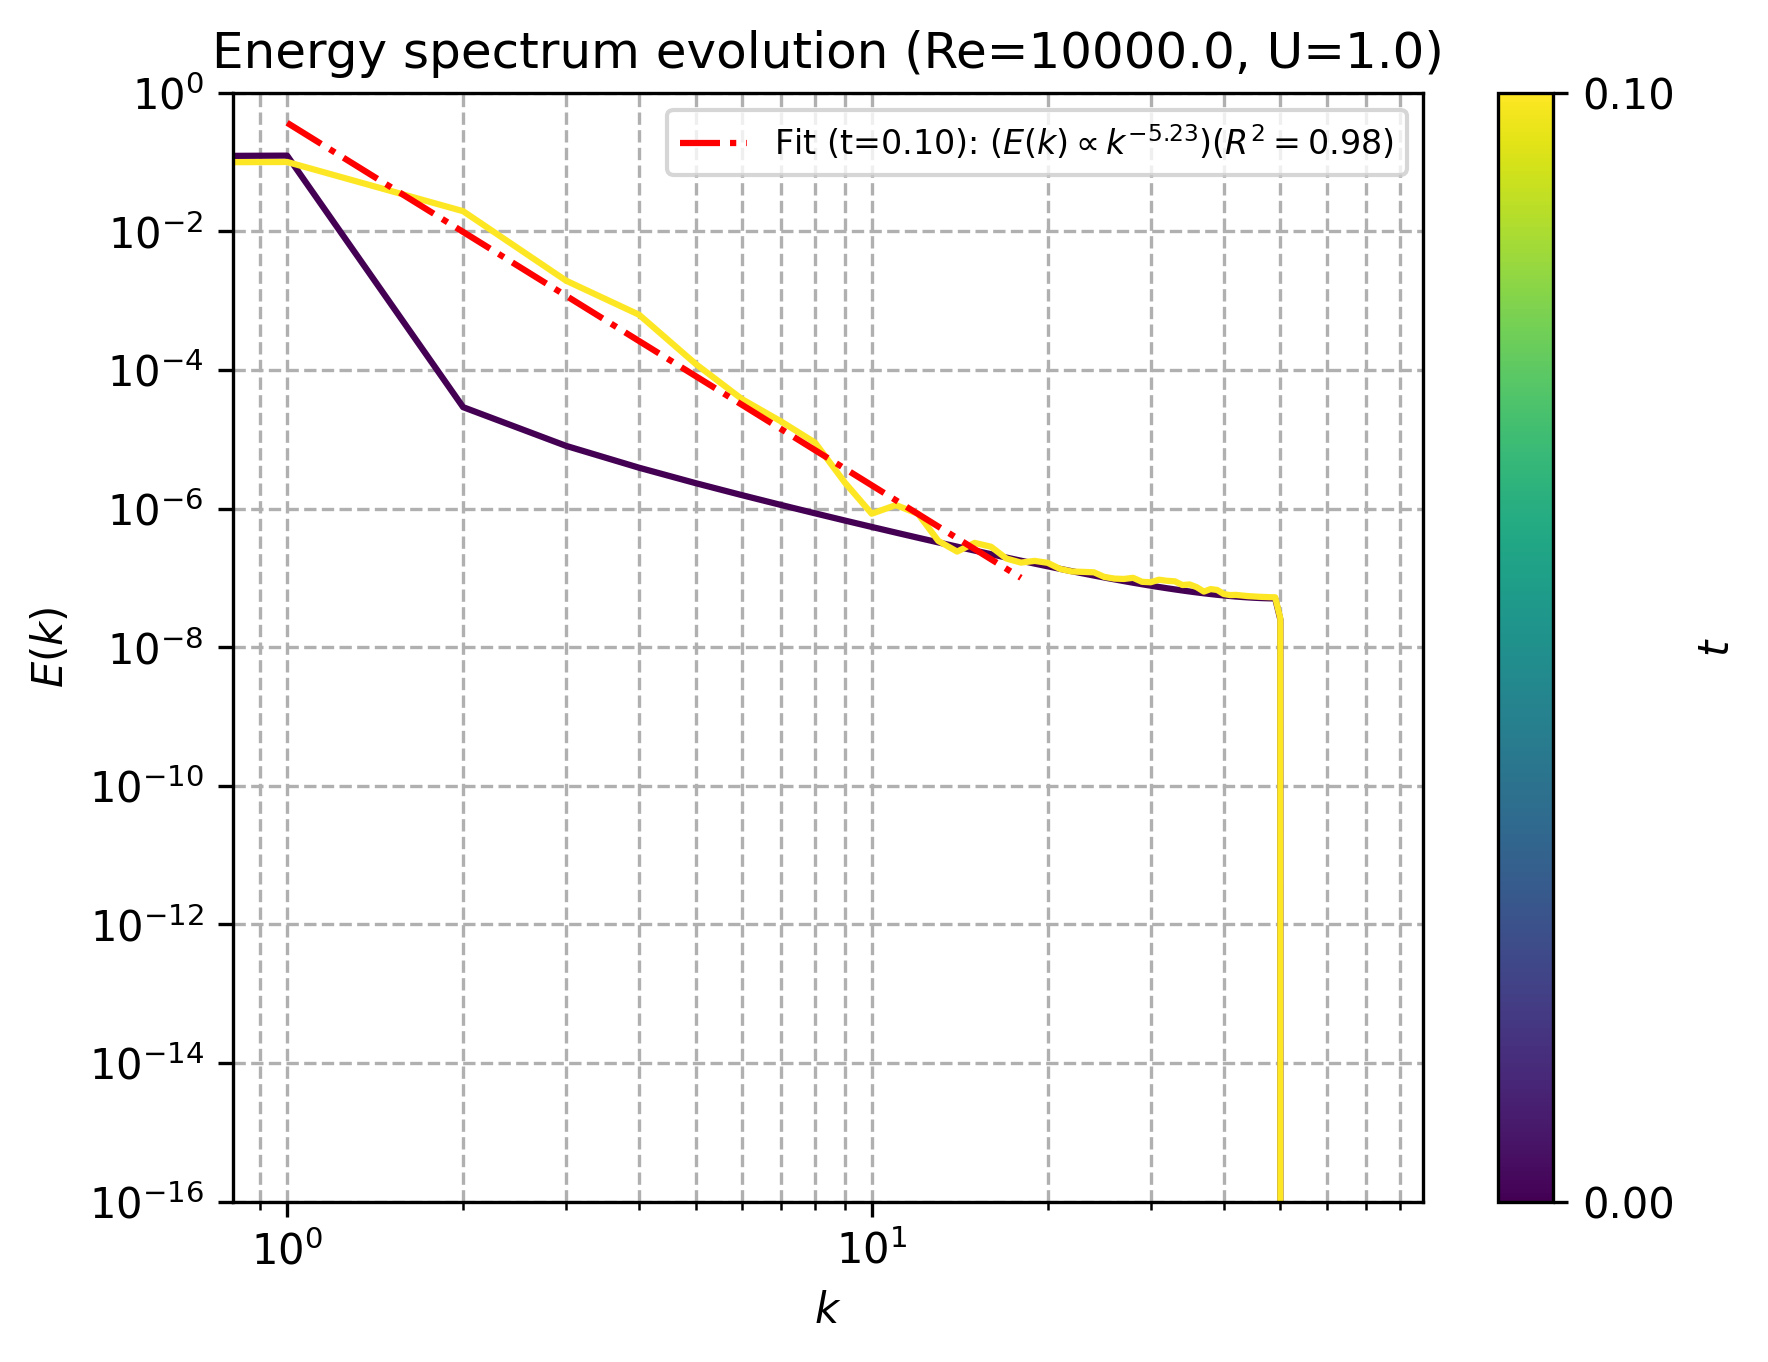
\includegraphics[width=6cm]{Code-Figures/okra2022/pst/c0_20_tait_pec_dtmul_1_nx_100_pst_-1_re_10000_ok2022/energy_spectrum_evolution.png}
    \caption{No PST}
  \end{subfigure}
  \begin{subfigure}{7cm}
    \centering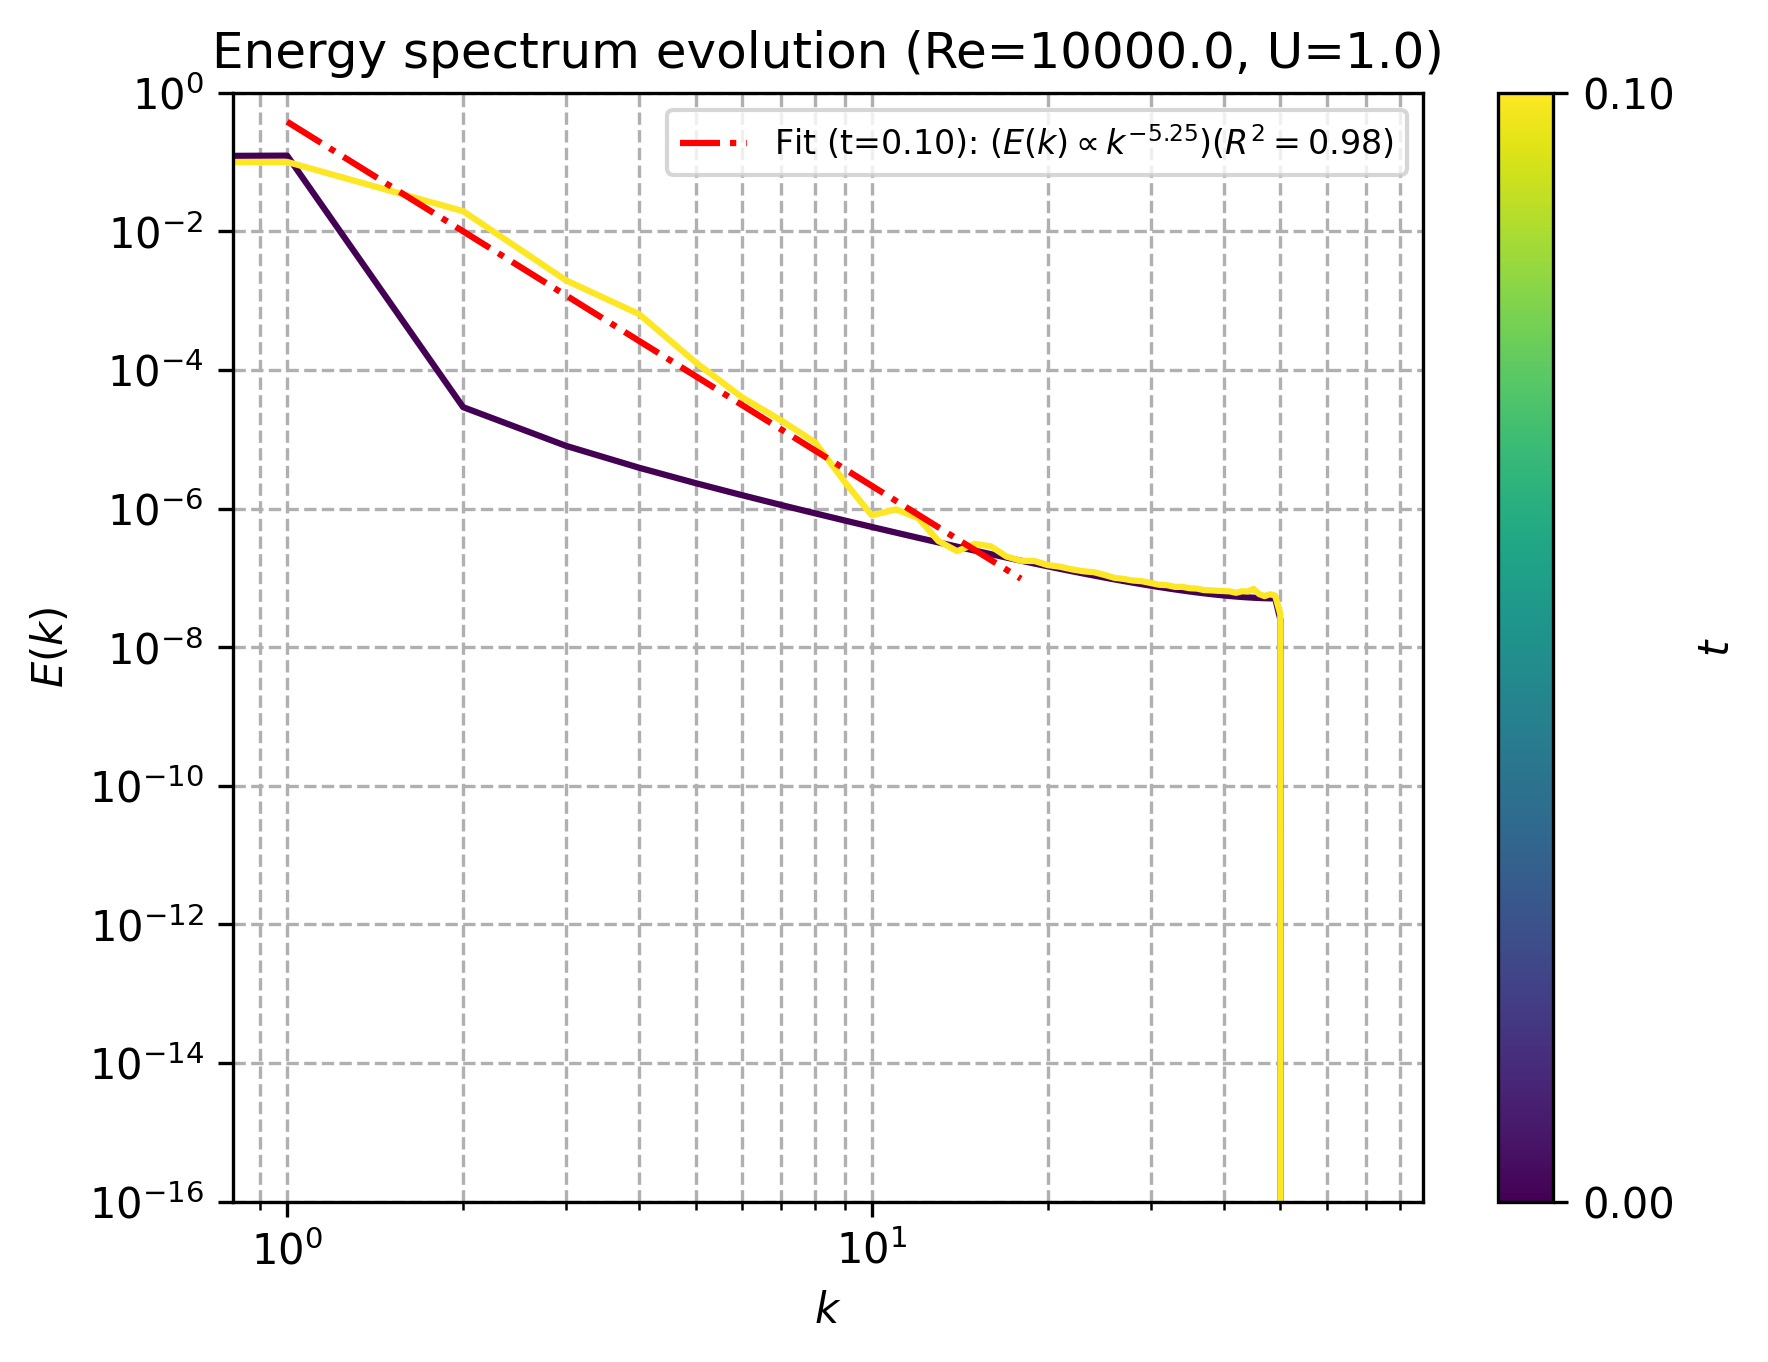
\includegraphics[width=6cm]{Code-Figures/okra2022/pst/c0_20_tait_pec_dtmul_1_nx_100_pst_10_re_10000_ok2022/energy_spectrum_evolution.png}
    \caption{$f_{pst} = 10$}
  \end{subfigure}
  \begin{subfigure}{7cm}
    \centering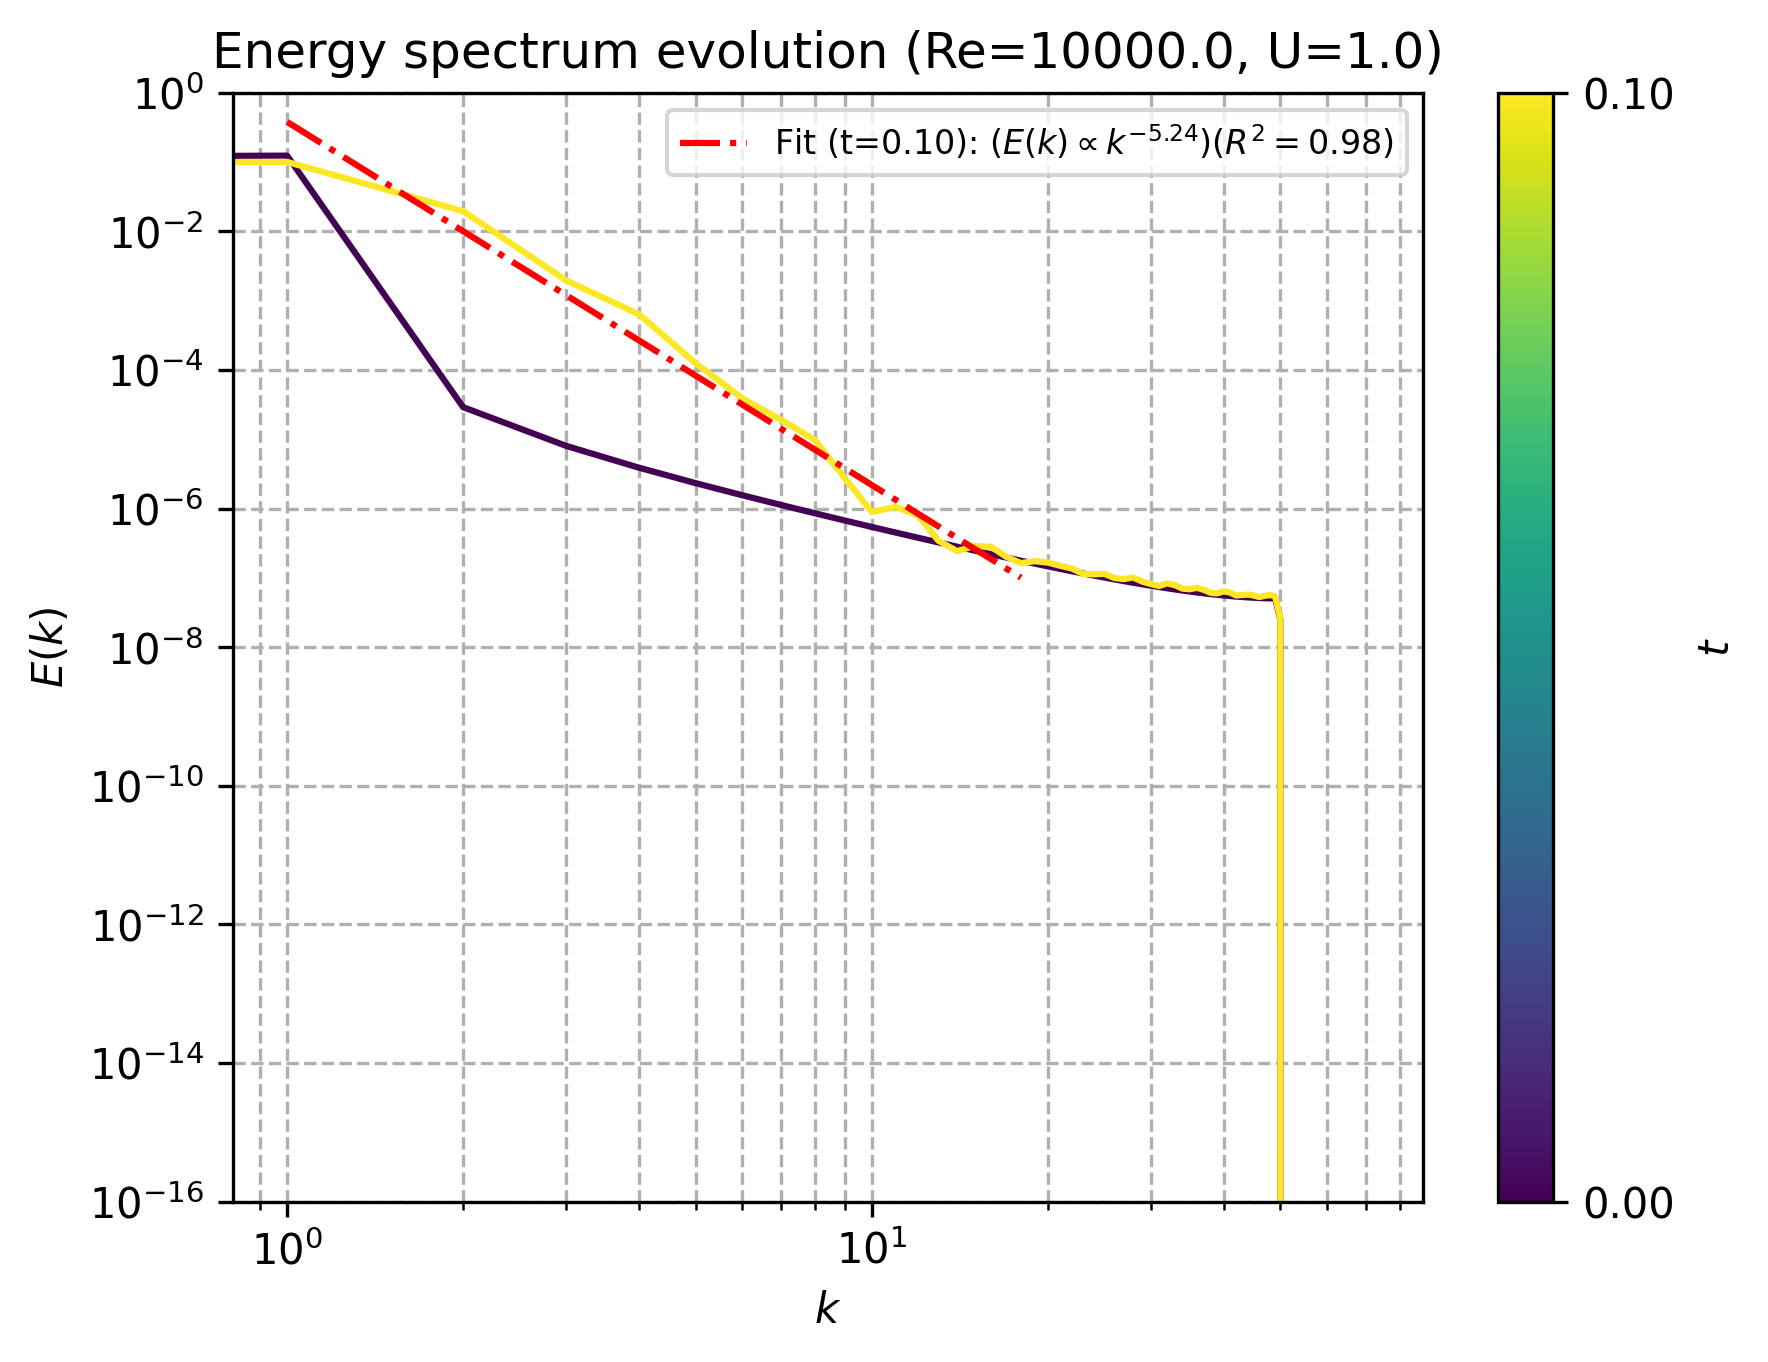
\includegraphics[width=6cm]{Code-Figures/okra2022/pst/c0_20_tait_pec_dtmul_1_nx_100_pst_50_re_10000_ok2022/energy_spectrum_evolution.png}
    \caption{$f_{pst} = 50$}
  \end{subfigure}
  \begin{subfigure}{7cm}
    \centering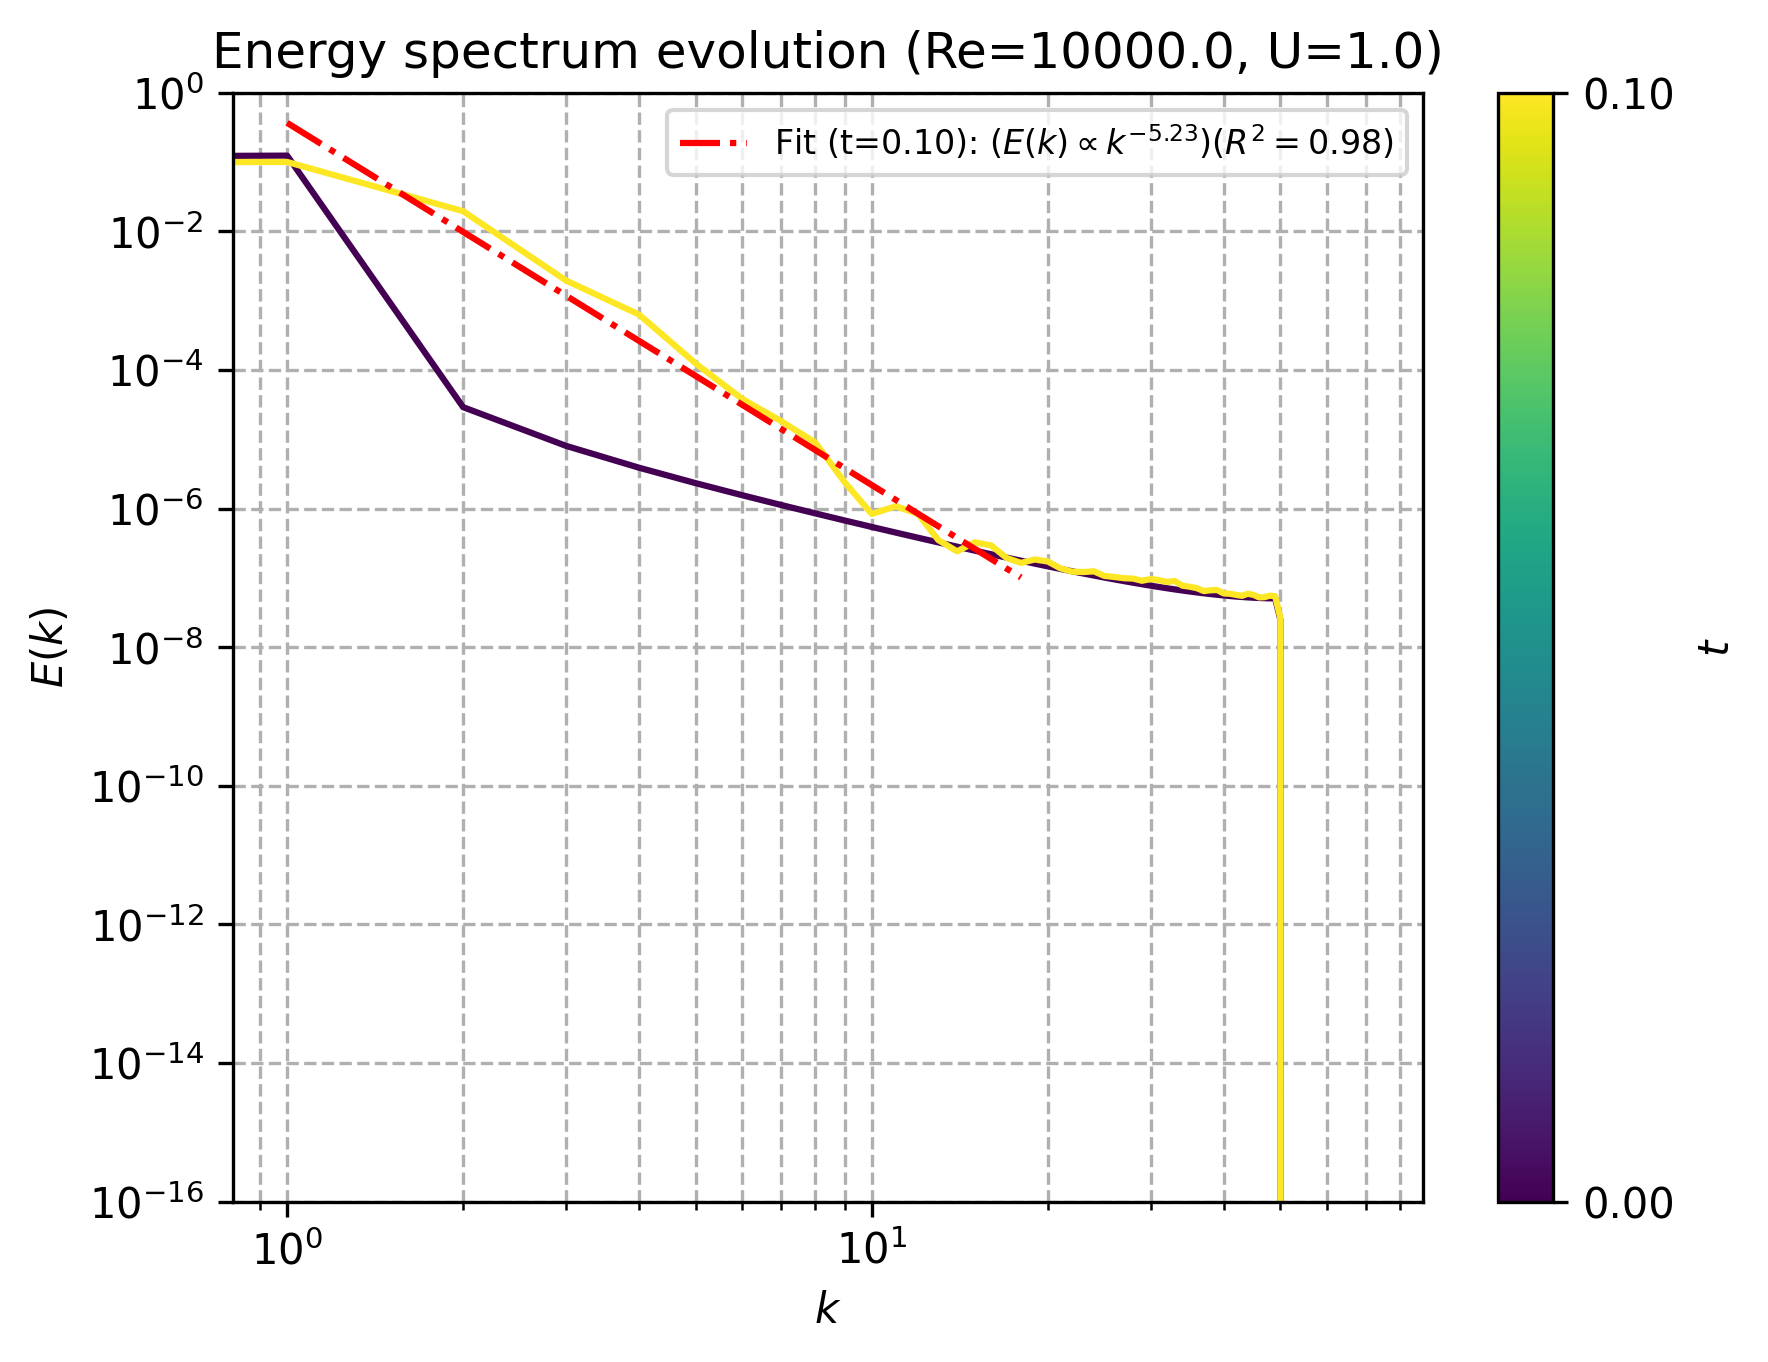
\includegraphics[width=6cm]{Code-Figures/okra2022/pst/c0_20_tait_pec_dtmul_1_nx_100_pst_100_re_10000_ok2022/energy_spectrum_evolution.png}
    \caption{$f_{pst} = 100$}
  \end{subfigure}
  \caption{Evolution of the energy spectrum for the SPH-LES scheme for various$f_{pst}$ values $(N=100^2, t_f=0.1, Re=10000, c_s=20)$. Initial energy spectrum is shown in dark blue, and the final energy spectrum is shown in yellow.}
  \label{fig:okra2022-pst-espec}
\end{figure}


\begin{figure}[H]
  \begin{subfigure}{7cm}
    \centering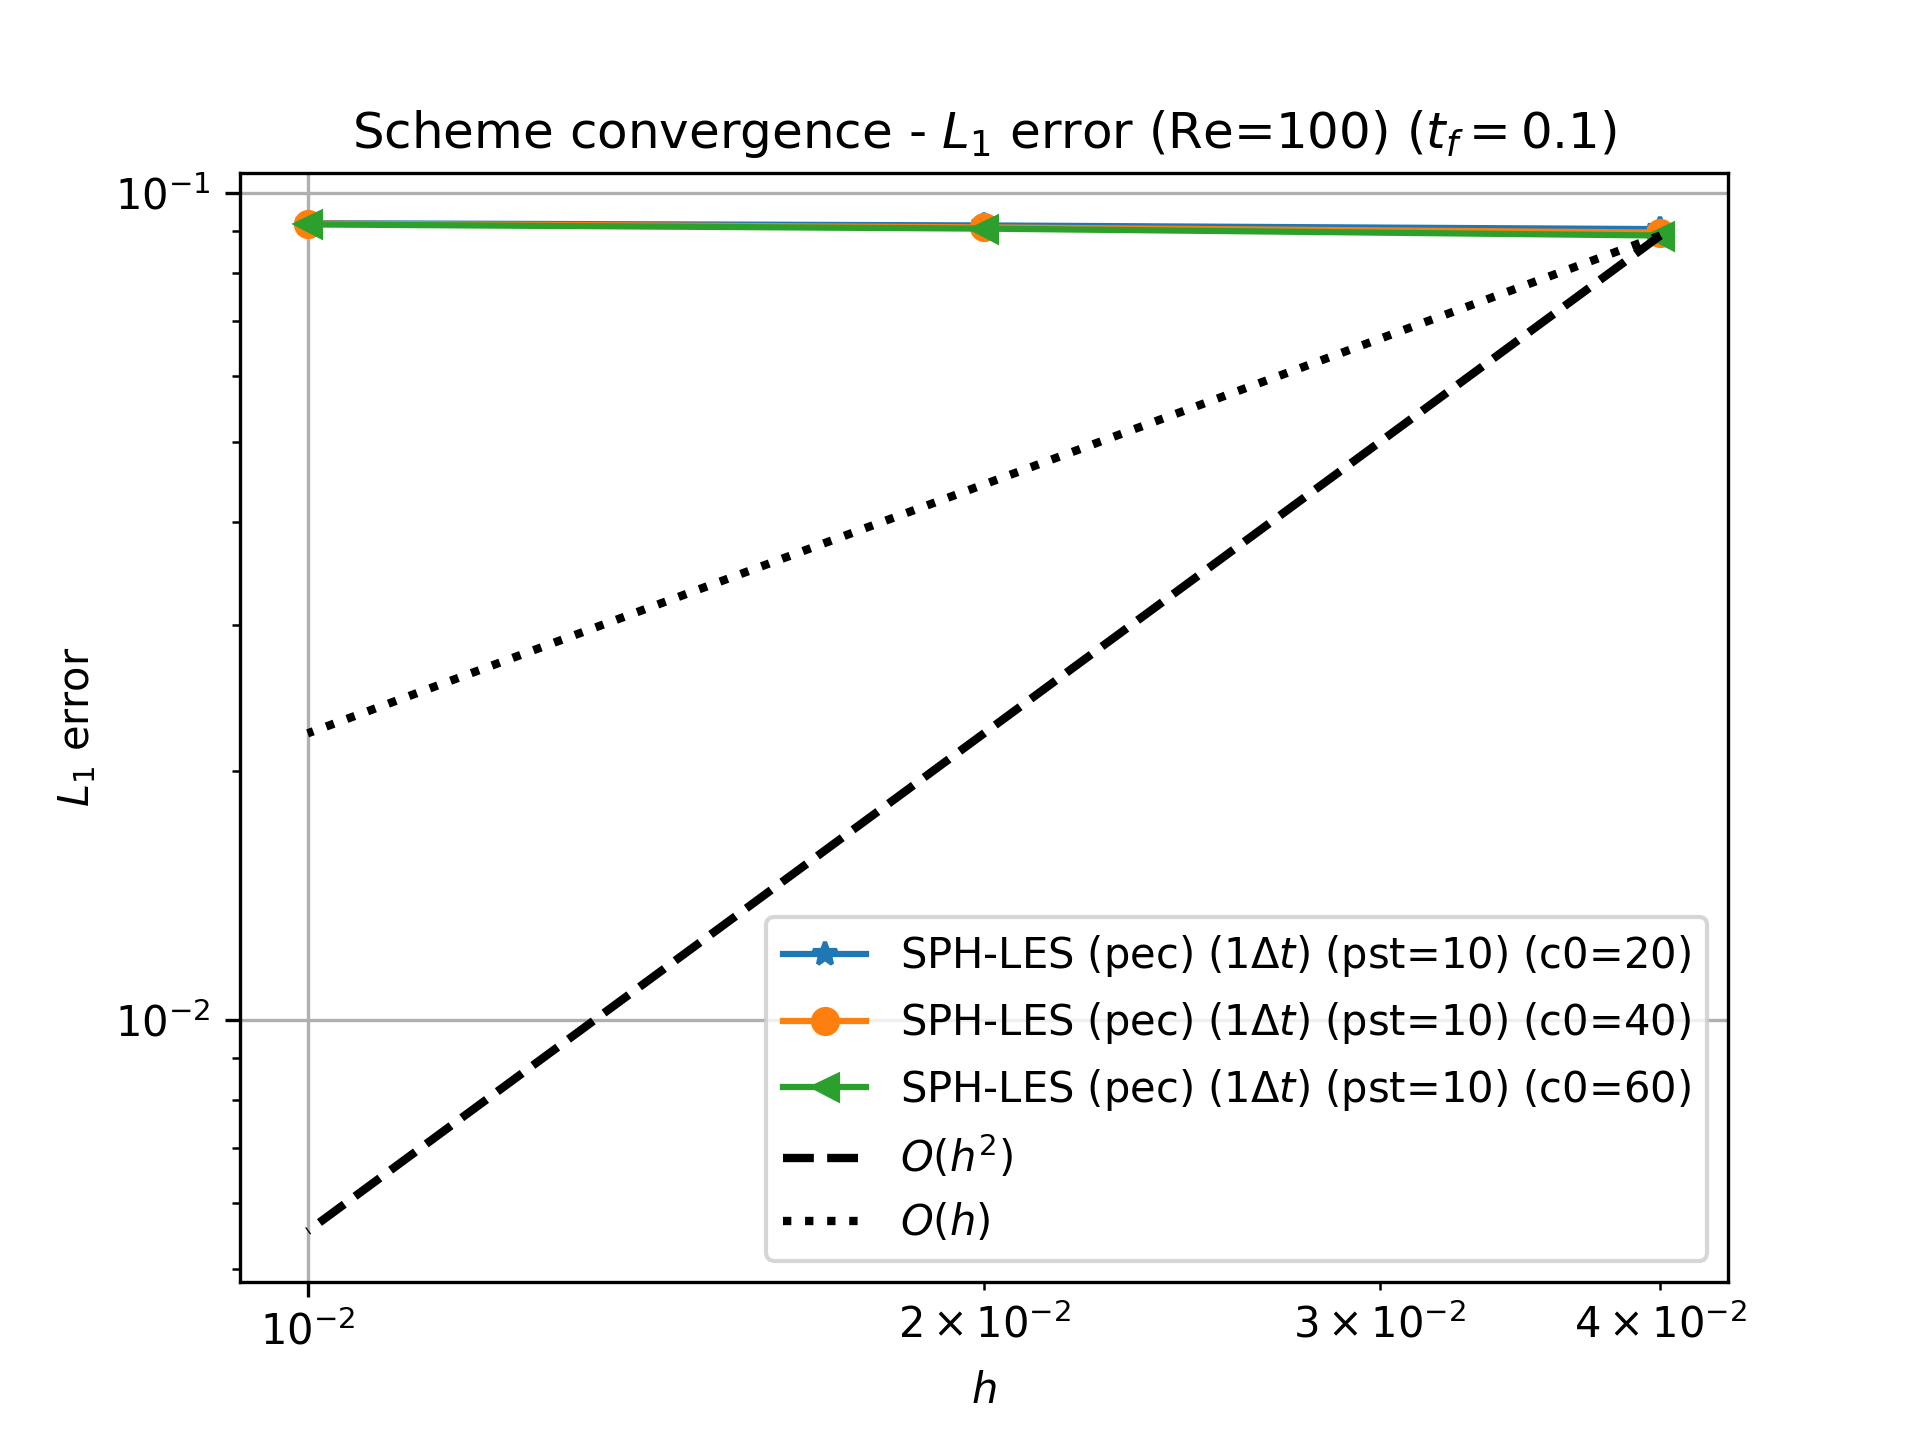
\includegraphics[width=6cm]{Code-Figures/okra2022/c0/dt_pois_conv_c0_pec_re_100.png}
    \caption{$Re = 100$}
  \end{subfigure}
  \begin{subfigure}{7cm}
    \centering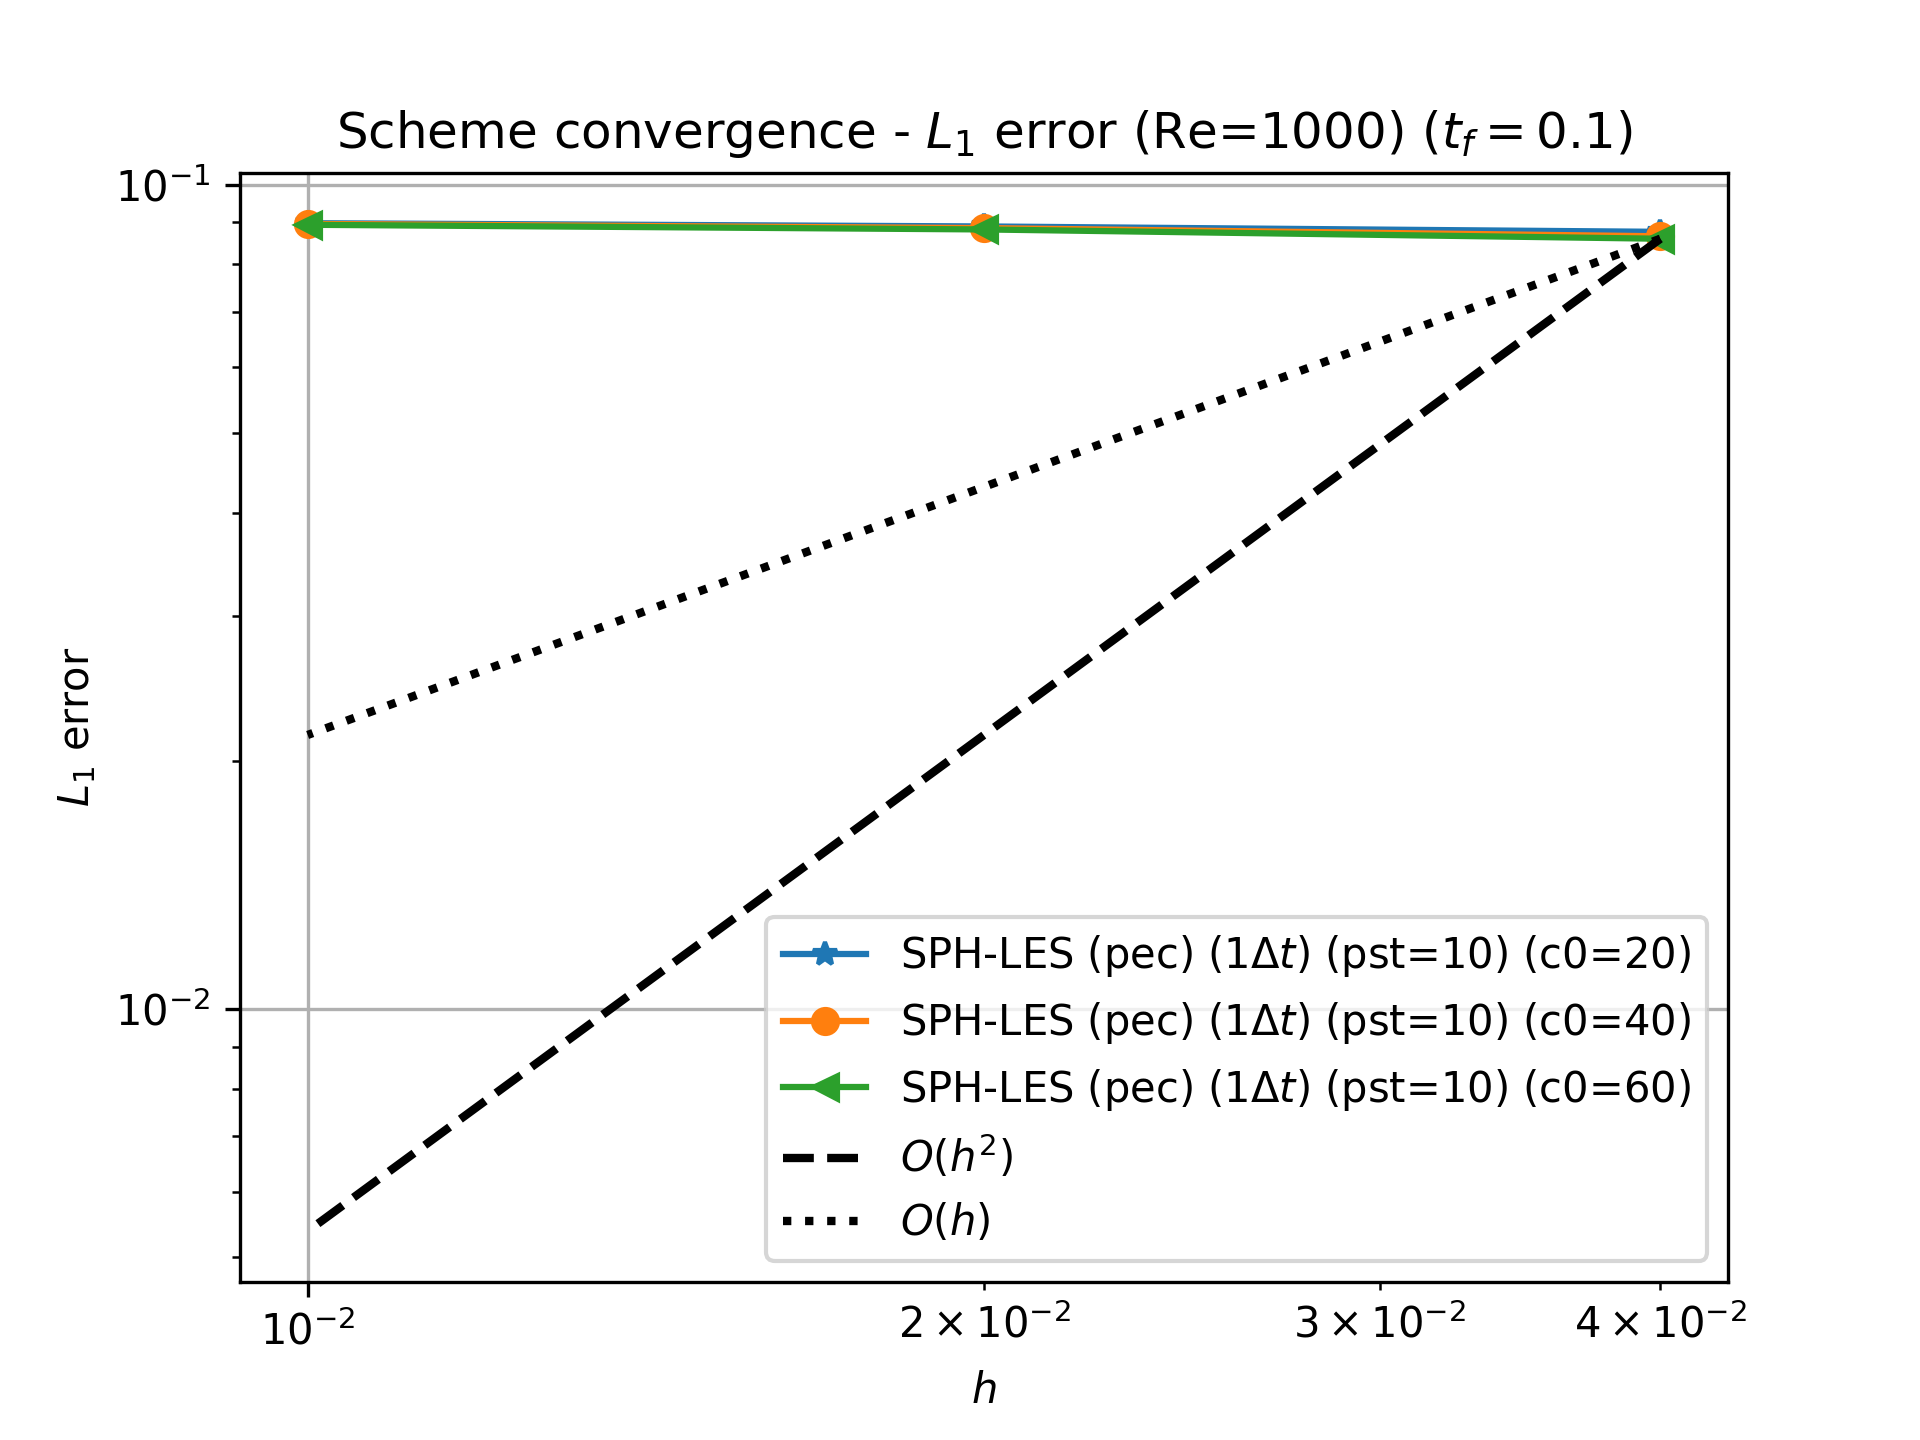
\includegraphics[width=6cm]{Code-Figures/okra2022/c0/dt_pois_conv_c0_pec_re_1000.png}
    \caption{$Re = 1000$}
  \end{subfigure}
  \begin{subfigure}{7cm}
    \centering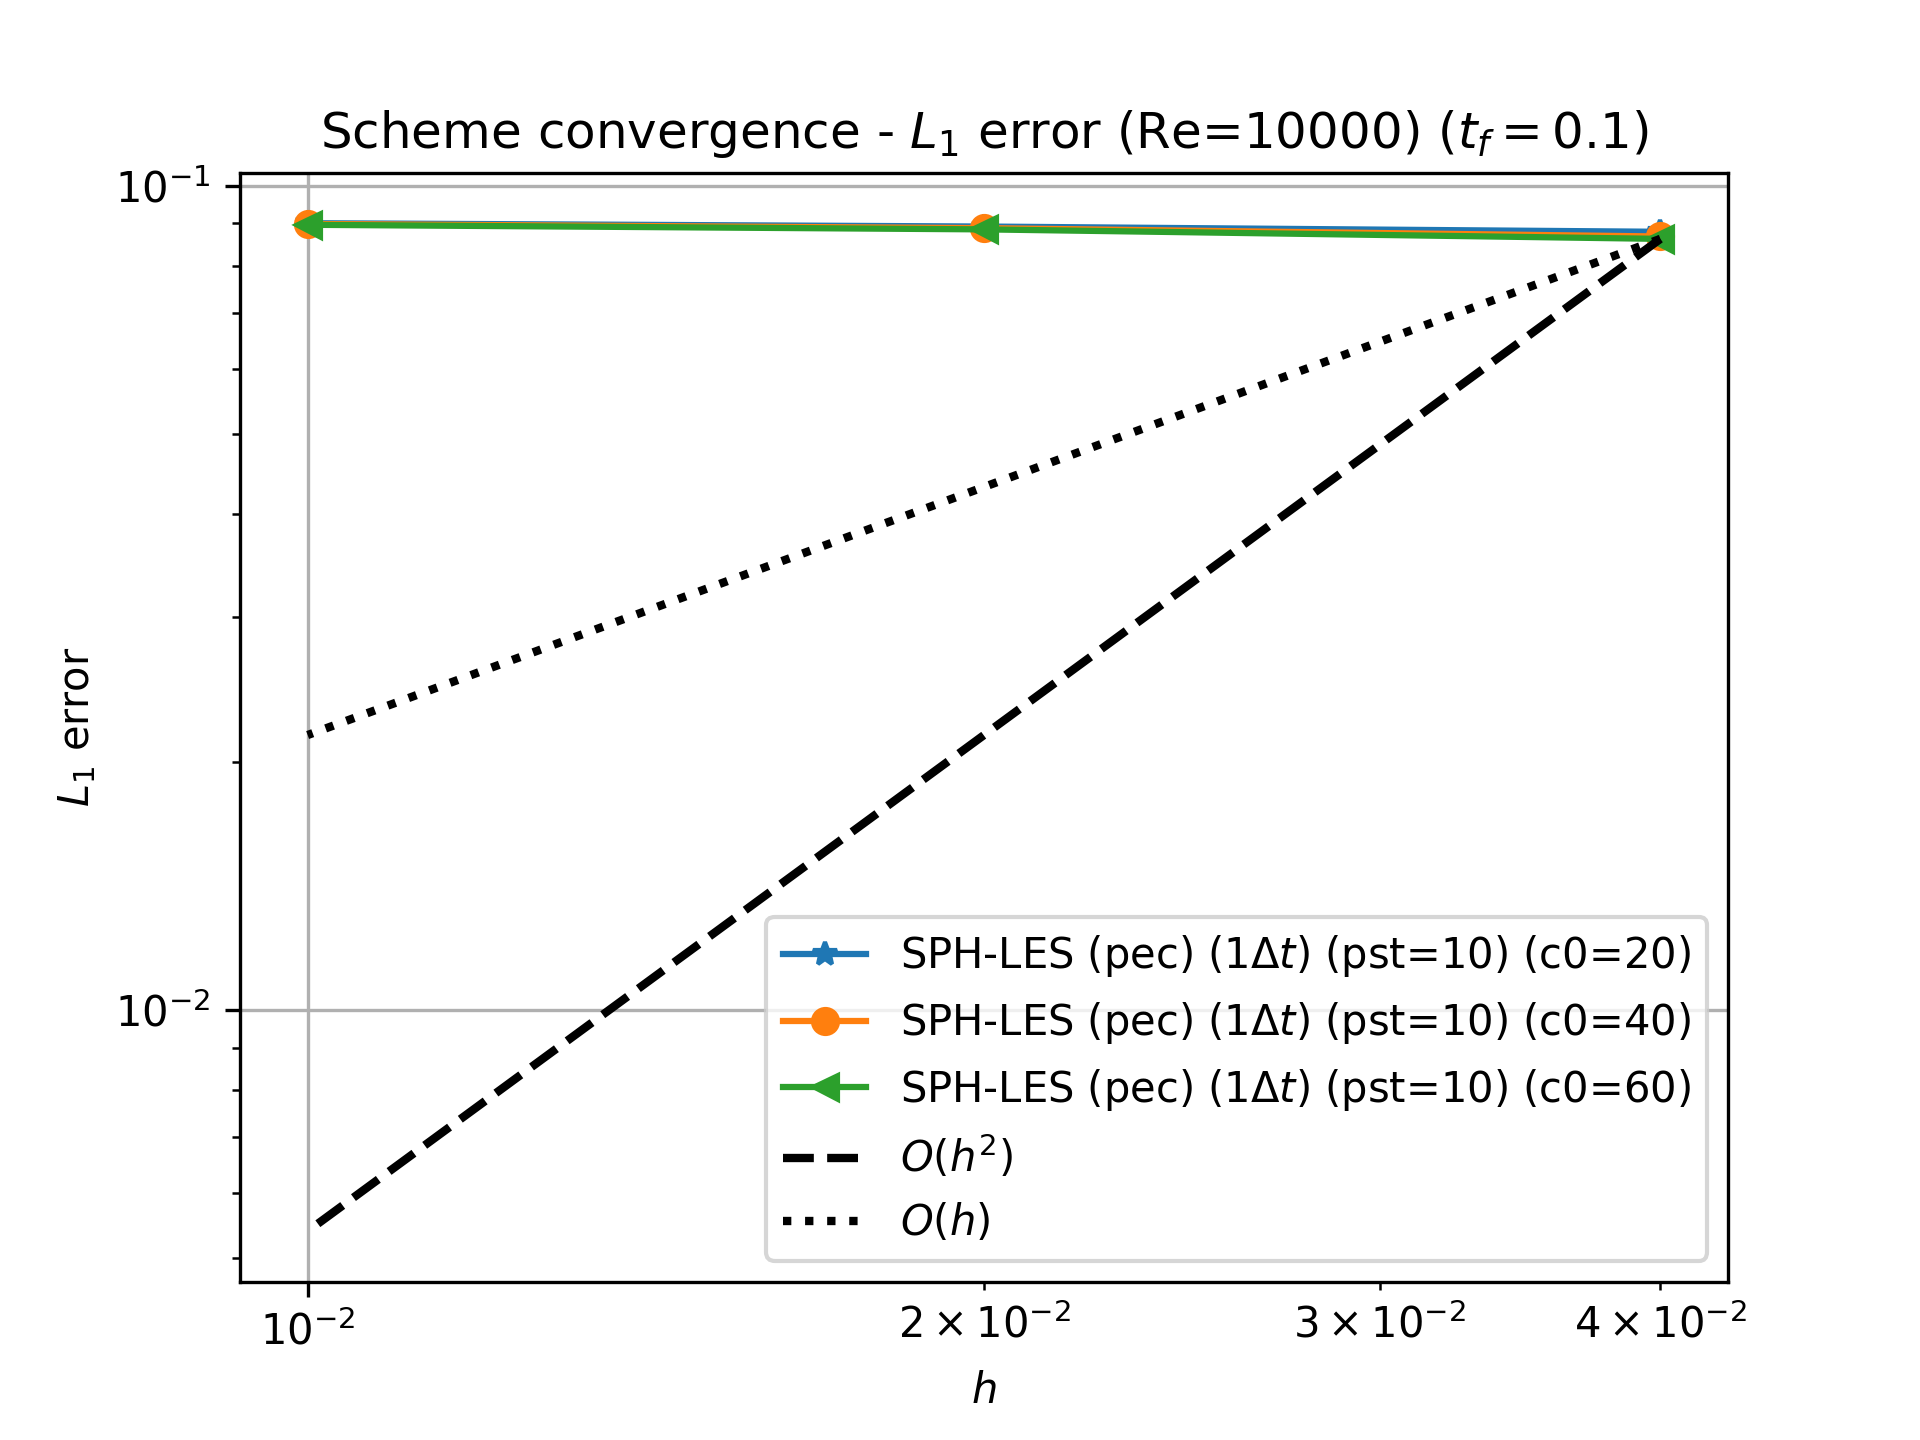
\includegraphics[width=6cm]{Code-Figures/okra2022/c0/dt_pois_conv_c0_pec_re_10000.png}
    \caption{$Re = 10000$}
  \end{subfigure}
  \caption{Convergence of the SPH-LES scheme for various speed of sound values.}
  \label{fig:okra2022-c0}
\end{figure}

In order to test the effect of the speed of sound on the scheme, the following values were considered: $c_s = [20, 40, 60]$. The results are shown in \figref{fig:okra2022-c0}, where it can again be seen that the scheme is zero order convergent, irrespective of the value of $c_s$.
In \figref{fig:okra2022-c0-vmag}, it can be observed that the higher $c_s$ values, which lead to smaller $\Delta t$ values, lead to a more uniformly distributed group of particles, while also leading to an increased $\abs{\vect{v}}_{max}$ value. This seems to add credence to the fact that increasing the resolution in the time domain, is dumping additional energy into the system as noise. This is also reflected in the energy spectrum shown in \figref{fig:okra2022-c0-espec}, where it can be observed that the slope of the energy spectrum, increases with increasing values of $c_s$.
Therefore, a value of $c_s = 20$ is chosen as the default value for the speed of sound, with the caveat that this scheme, possibly cannot be used for problems of lower $Re$ at all, since they require dissipation of energy, which does not appear to be the case for this scheme.

\begin{figure}[H]
  \begin{subfigure}{7cm}
    \centering\includegraphics[width=6cm]{Code-Figures/okra2022/c0/c0_20_tait_pec_dtmul_1_nx_50_pst_10_re_10000_ok2022/final_vmag.png}
    \caption{$c_s=20$}
  \end{subfigure}
  \begin{subfigure}{7cm}
    \centering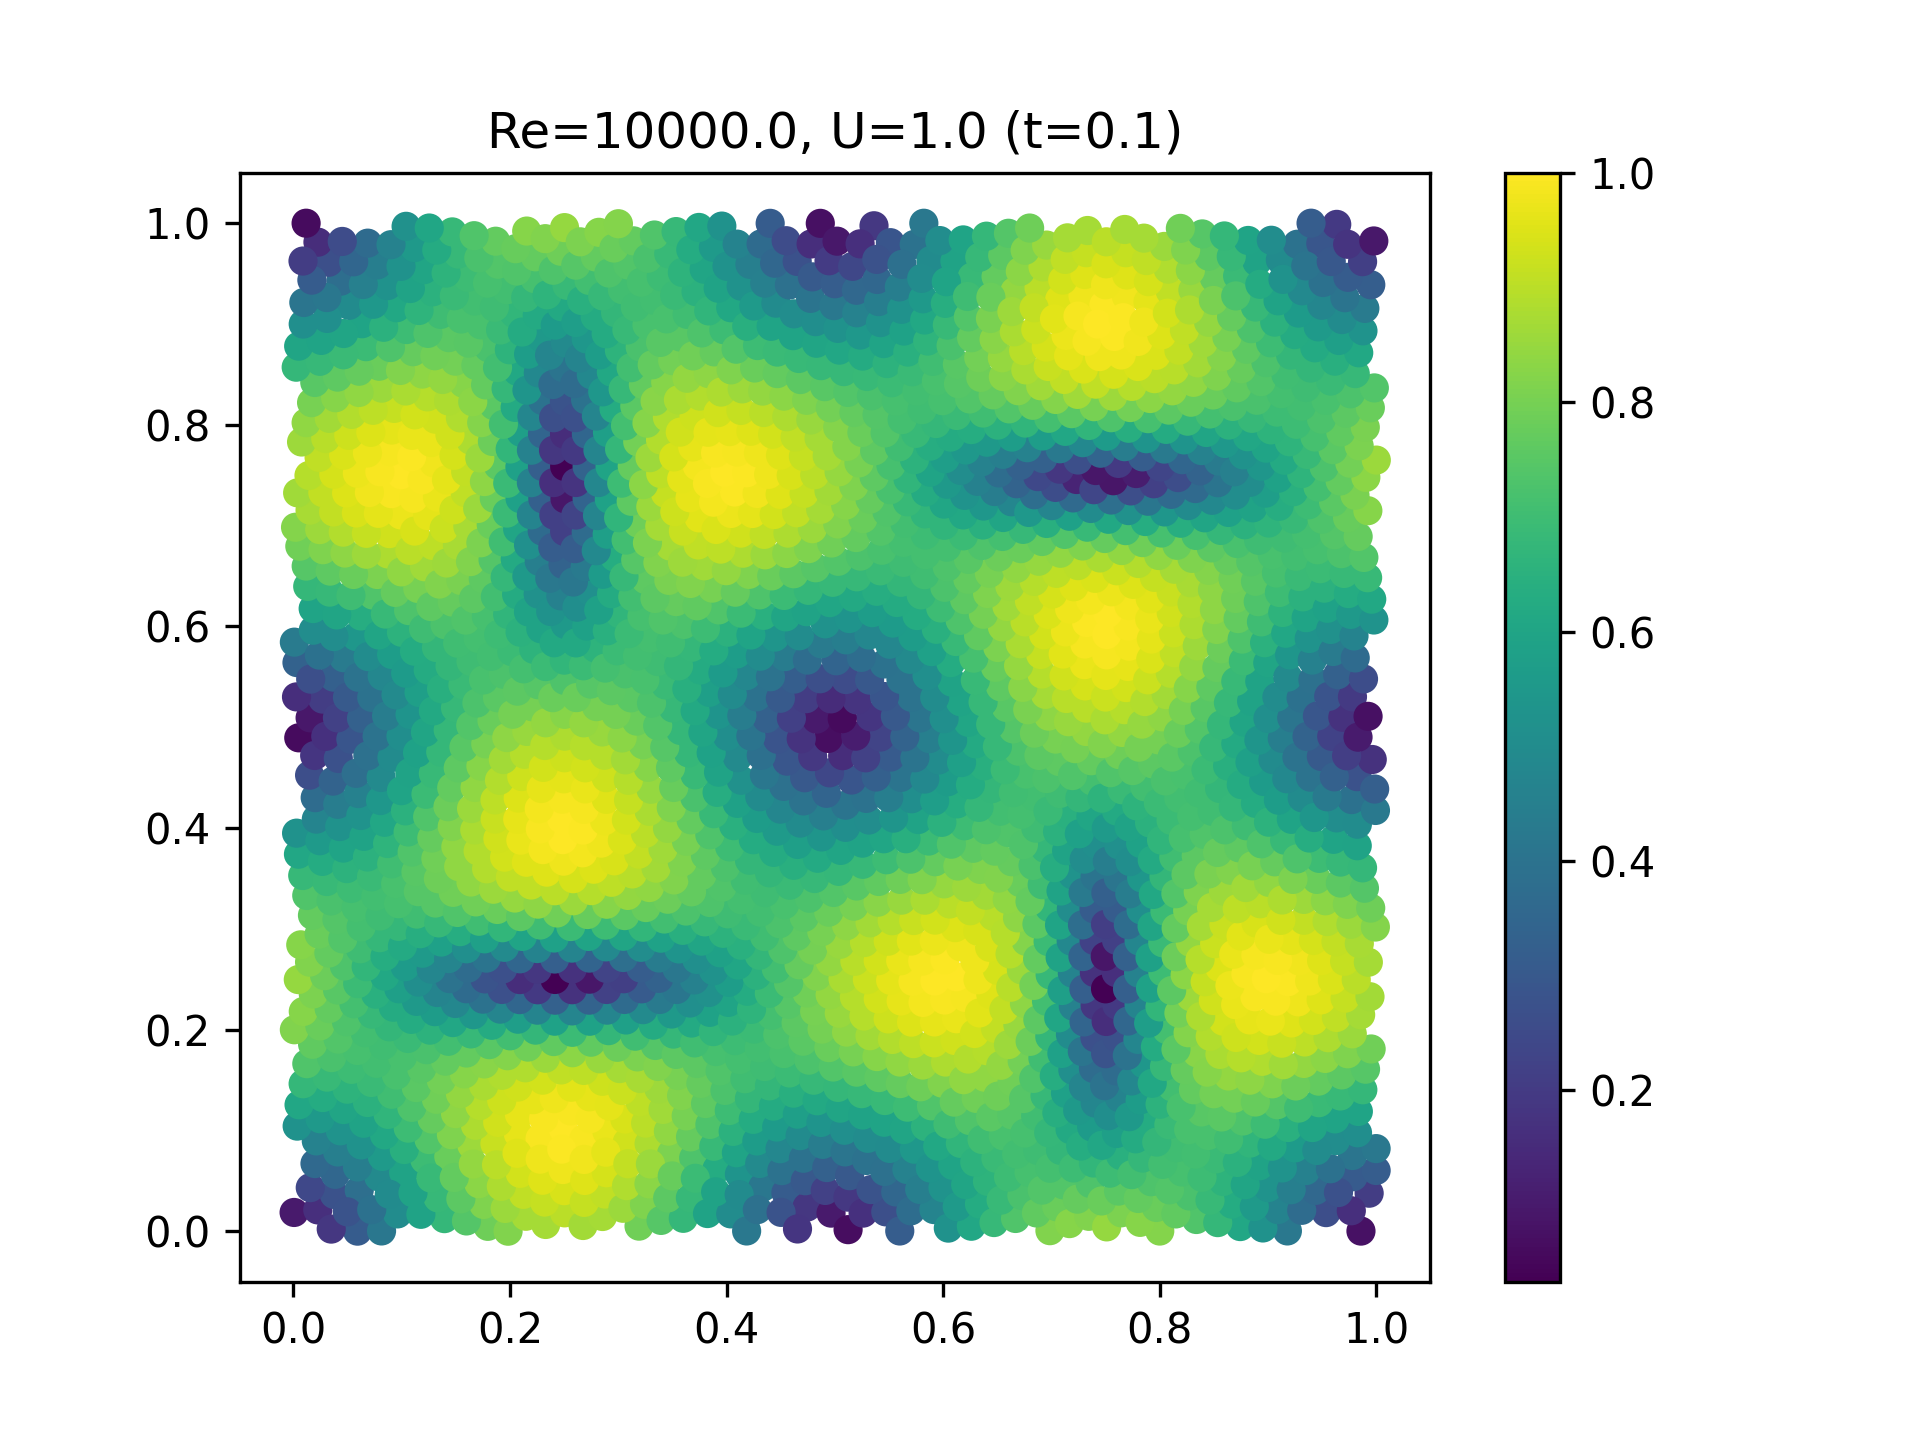
\includegraphics[width=6cm]{Code-Figures/okra2022/c0/c0_40_tait_pec_dtmul_1_nx_50_pst_10_re_10000_ok2022/final_vmag.png}
    \caption{$c_s=40$}
  \end{subfigure}
  \begin{subfigure}{7cm}
    \centering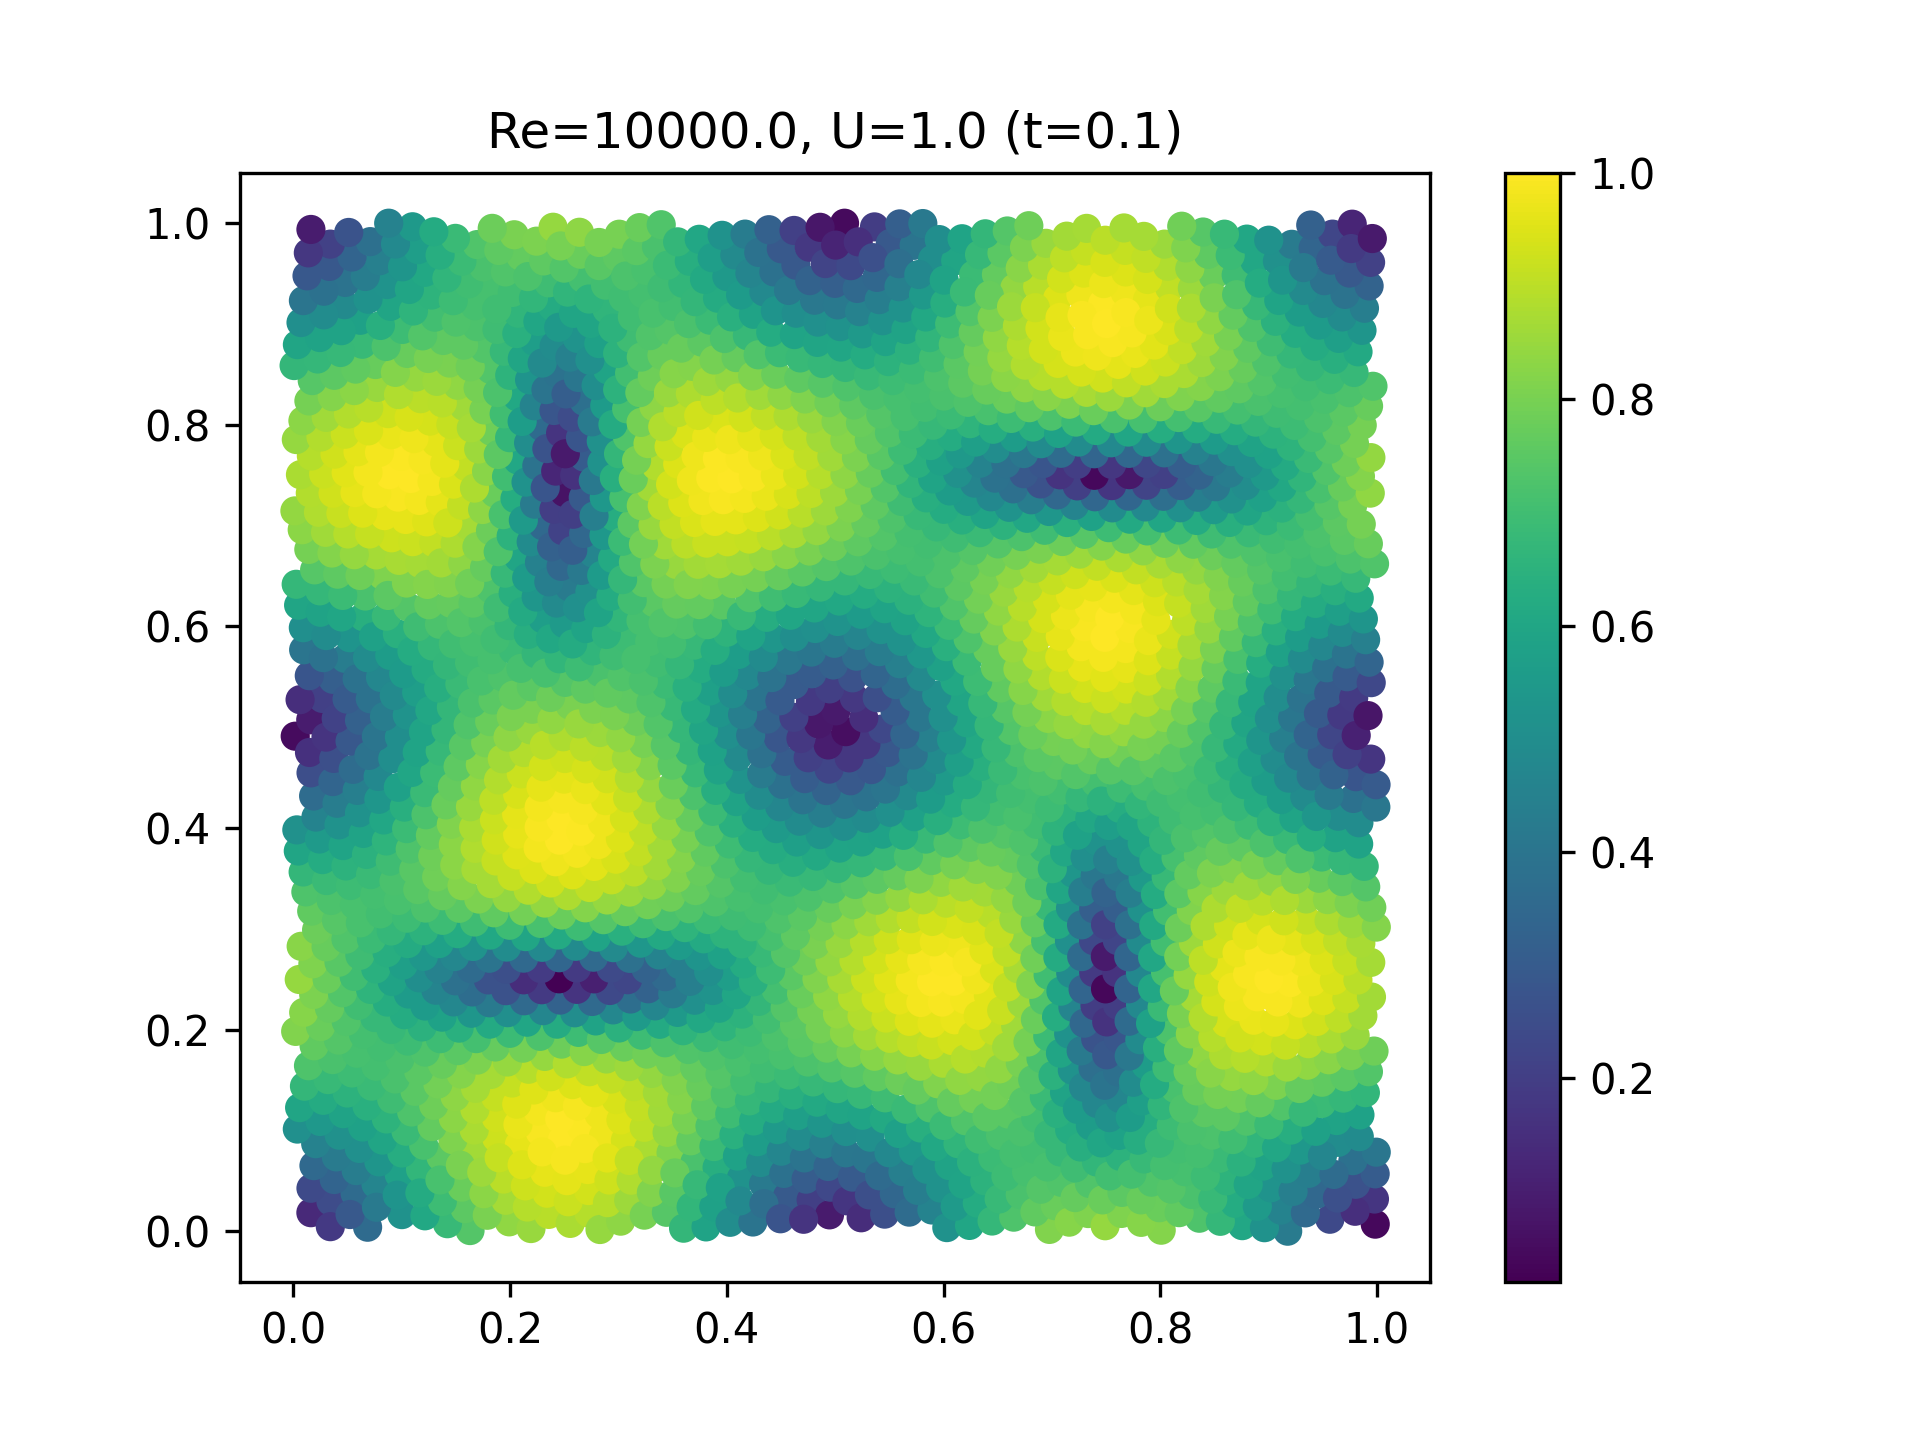
\includegraphics[width=6cm]{Code-Figures/okra2022/c0/c0_60_tait_pec_dtmul_1_nx_50_pst_10_re_10000_ok2022/final_vmag.png}
    \caption{$c_s=60$}
  \end{subfigure}
  \caption{Velocity magnitude field for the SPH-LES scheme for various speed of sound values $(N=50^2, t_f=0.1, Re=10000, f_{pst}=10)$.}
  \label{fig:okra2022-c0-vmag}
\end{figure}

\begin{figure}[H]
  \begin{subfigure}{7cm}
    \centering\includegraphics[width=6cm]{Code-Figures/okra2022/c0/c0_20_tait_pec_dtmul_1_nx_100_pst_10_re_10000_ok2022/energy_spectrum_evolution.png}
    \caption{$c_s=20$}
  \end{subfigure}
  \begin{subfigure}{7cm}
    \centering\includegraphics[width=6cm]{Code-Figures/okra2022/c0/c0_40_tait_pec_dtmul_1_nx_100_pst_10_re_10000_ok2022/energy_spectrum_evolution.png}
    \caption{$c_s=40$}
  \end{subfigure}
  \begin{subfigure}{7cm}
    \centering\includegraphics[width=6cm]{Code-Figures/okra2022/c0/c0_60_tait_pec_dtmul_1_nx_100_pst_10_re_10000_ok2022/energy_spectrum_evolution.png}
    \caption{$c_s=60$}
  \end{subfigure}
  \caption{Evolution of the energy spectrum for the SPH-LES scheme for various speed of sound values $(N=100^2, t_f=0.1, Re=10000, f_{pst}=10)$.}
  \label{fig:okra2022-c0-espec}
\end{figure}

Hence, it can be concluded that the SPH-LES scheme is not suitable for problems of low $Re$, due to firstly the lack of dissipation of energy, and secondly, it being zero order-convergent. For the cases of high $Re$, the scheme again would require a lot more testing for each specific problem, before it the flow field can be considered to be accurate. This is refected in the velocity magnitude plots show in \figref{fig:okra2022-pst-vmag} and \figref{fig:okra2022-c0-vmag}, where the flow field at the final time instance, is not the expected Taylor-Green profile, and instead distorted vortex structures are observed.


\subsection{$\delta$-LES-SPH Scheme}
The Lagrangian LES-based models, have only two major schemes to offer. One being the LES-SPH scheme of \cite{DiMascio2017} and the other being the $\delta$-LES-SPH scheme of \cite{Colagrossi2021QuasiLagrangian}.
The latter was chosen, since their scheme introduced a small arbitrary velocity deviation $(\TildeDeltaV)$ to the fluid particles, which allowed for improved accuracy in simulations of high Reynolds number problems. This scheme, also included the use of PST and tensile instability control (TIC). All of this allowed the scheme to tackle without facing the issue of spurious high-frequency noise and the onset of the tensile instability, and hence was chosen.

The $k-\epsilon$ SPH scheme of \cite{Shao2006} was chosen over the other RANS-based schemes, since it was straightforward in terms of the governing equations involved.

Delta LES SPH RHO - EOS \figref{fig:deltales_sd-eos}
\begin{figure}[H]
  \begin{subfigure}{7cm}
    \centering\includegraphics[width=6cm]{Code-Figures/deltales_sd/eos/dt_pois_conv_c0_20_re_100.png}
    \caption{$Re = 100$}
  \end{subfigure}
  \begin{subfigure}{7cm}
    \centering\includegraphics[width=6cm]{Code-Figures/deltales_sd/eos/dt_pois_conv_c0_20_re_1000.png}
    \caption{$Re = 1000$}
  \end{subfigure}
  \begin{subfigure}{7cm}
    \centering\includegraphics[width=6cm]{Code-Figures/deltales_sd/eos/dt_pois_conv_c0_20_re_10000.png}
    \caption{$Re = 10000$}
  \end{subfigure}
  \caption{Convergence of the $\delta$-LES-SPH $(\rho)$ scheme for various equations of state.}
  \label{fig:deltales_sd-eos}
\end{figure}


Delta LES SPH RHOC - EOS \figref{fig:deltales-eos}
\begin{figure}[H]
  \begin{subfigure}{7cm}
    \centering\includegraphics[width=6cm]{Code-Figures/deltales/eos/dt_pois_conv_c0_20_re_100.png}
    \caption{$Re = 100$}
  \end{subfigure}
  \begin{subfigure}{7cm}
    \centering\includegraphics[width=6cm]{Code-Figures/deltales/eos/dt_pois_conv_c0_20_re_1000.png}
    \caption{$Re = 1000$}
  \end{subfigure}
  \begin{subfigure}{7cm}
    \centering\includegraphics[width=6cm]{Code-Figures/deltales/eos/dt_pois_conv_c0_20_re_10000.png}
    \caption{$Re = 10000$}
  \end{subfigure}
  \caption{Convergence of the $\delta$-LES-SPH $(\rho_c)$ scheme for various equations of state.}
  \label{fig:deltales-eos}
\end{figure}


Delta LES SPH RHOC - PST \figref{fig:deltales-pst}
\begin{figure}[H]
  \begin{subfigure}{7cm}
    \centering\includegraphics[width=6cm]{Code-Figures/deltales/pst/dt_pois_conv_c0_20_re_100.png}
    \caption{$Re = 100$}
  \end{subfigure}
  \begin{subfigure}{7cm}
    \centering\includegraphics[width=6cm]{Code-Figures/deltales/pst/dt_pois_conv_c0_20_re_1000.png}
    \caption{$Re = 1000$}
  \end{subfigure}
  \begin{subfigure}{7cm}
    \centering\includegraphics[width=6cm]{Code-Figures/deltales/pst/dt_pois_conv_c0_20_re_10000.png}
    \caption{$Re = 10000$}
  \end{subfigure}
  \caption{Convergence of the $\delta$-LES-SPH $(\rho_c)$ scheme for various $f_{pst}$ values.}
  \label{fig:deltales-pst}
\end{figure}


Delta LES SPH RHOC - PST VMAG \figref{fig:deltales-pst-vmag}
\begin{figure}[H]
  \begin{subfigure}{7cm}
    \centering\includegraphics[width=6cm]{Code-Figures/deltales/pst/c0_20_tait_pec_dtmul_1_nx_50_pst_-1_re_10000_deltales/final_vmag.png}
    \caption{No PST}
  \end{subfigure}
  \begin{subfigure}{7cm}
    \centering\includegraphics[width=6cm]{Code-Figures/deltales/pst/c0_20_tait_pec_dtmul_1_nx_50_pst_10_re_10000_deltales/final_vmag.png}
    \caption{$f_{pst} = 10$}
  \end{subfigure}
  \begin{subfigure}{7cm}
    \centering\includegraphics[width=6cm]{Code-Figures/deltales/pst/c0_20_tait_pec_dtmul_1_nx_50_pst_50_re_10000_deltales/final_vmag.png}
    \caption{$f_{pst} = 50$}
  \end{subfigure}
  \begin{subfigure}{7cm}
    \centering\includegraphics[width=6cm]{Code-Figures/deltales/pst/c0_20_tait_pec_dtmul_1_nx_50_pst_100_re_10000_deltales/final_vmag.png}
    \caption{$f_{pst} = 100$}
  \end{subfigure}
  \caption{Velocity magnitude field for the $\delta$-LES-SPH $(\rho_c)$ scheme for various $f_{pst}$ values $(N=50^2, t_f=0.1, Re=10000, c_s=20)$.}
  \label{fig:deltales-pst-vmag}
\end{figure}


Delta LES SPH RHOC - PST ESPEC \figref{fig:deltales-pst-espec}
\begin{figure}[H]
  \begin{subfigure}{7cm}
    \centering\includegraphics[width=6cm]{Code-Figures/deltales/pst/c0_20_tait_pec_dtmul_1_nx_100_pst_-1_re_10000_deltales/energy_spectrum_evolution.png}
    \caption{No PST}
  \end{subfigure}
  \begin{subfigure}{7cm}
    \centering\includegraphics[width=6cm]{Code-Figures/deltales/pst/c0_20_tait_pec_dtmul_1_nx_100_pst_10_re_10000_deltales/energy_spectrum_evolution.png}
    \caption{$f_{pst} = 10$}
  \end{subfigure}
  \begin{subfigure}{7cm}
    \centering\includegraphics[width=6cm]{Code-Figures/deltales/pst/c0_20_tait_pec_dtmul_1_nx_100_pst_50_re_10000_deltales/energy_spectrum_evolution.png}
    \caption{$f_{pst} = 50$}
  \end{subfigure}
  \begin{subfigure}{7cm}
    \centering\includegraphics[width=6cm]{Code-Figures/deltales/pst/c0_20_tait_pec_dtmul_1_nx_100_pst_100_re_10000_deltales/energy_spectrum_evolution.png}
    \caption{$f_{pst} = 100$}
  \end{subfigure}
  \caption{Evolution of the energy spectrum for the $\delta$-LES-SPH $(\rho_c)$ scheme for various $f_{pst}$ values $(N=100^2, t_f=0.1, Re=10000, c_s=20)$. Initial energy spectrum is shown in dark blue, and the final energy spectrum is shown in yellow.}
  \label{fig:deltales-pst-espec}
\end{figure}


Delta LES SPH RHOC - INTEGRATOR \figref{fig:deltales-integrator}
\begin{figure}[H]
  \begin{subfigure}{7cm}
    \centering\includegraphics[width=6cm]{Code-Figures/deltales/integrator/dt_pois_conv_c0_20_re_100.png}
    \caption{$Re = 100$}
  \end{subfigure}
  \begin{subfigure}{7cm}
    \centering\includegraphics[width=6cm]{Code-Figures/deltales/integrator/dt_pois_conv_c0_20_re_1000.png}
    \caption{$Re = 1000$}
  \end{subfigure}
  \begin{subfigure}{7cm}
    \centering\includegraphics[width=6cm]{Code-Figures/deltales/integrator/dt_pois_conv_c0_20_re_10000.png}
    \caption{$Re = 10000$}
  \end{subfigure}
  \caption{Convergence of the $\delta$-LES-SPH $(\rho_c)$ scheme for various time-integration schemes.}
  \label{fig:deltales-integrator}
\end{figure}


Delta LES SPH RHOC - INTEGRATOR VMAG \figref{fig:deltales-integrator-vmag}
\begin{figure}[H]
  \begin{subfigure}{7cm}
    \centering\includegraphics[width=6cm]{Code-Figures/deltales/integrator/c0_20_tait_pec_dtmul_1_nx_50_pst_100_re_10000_deltales/final_vmag.png}
    \caption{\texttt{PEC}}
  \end{subfigure}
  \begin{subfigure}{7cm}
    \centering\includegraphics[width=6cm]{Code-Figures/deltales/integrator/c0_20_tait_rk2_dtmul_1.5_nx_50_pst_100_re_10000_deltales/final_vmag.png}
    \caption{\texttt{RK2}}
  \end{subfigure}
  \begin{subfigure}{7cm}
    \centering\includegraphics[width=6cm]{Code-Figures/deltales/integrator/c0_20_tait_rk4_dtmul_2_nx_50_pst_100_re_10000_deltales/final_vmag.png}
    \caption{\texttt{RK4}}
  \end{subfigure}
  \caption{Velocity magnitude field for the $\delta$-LES-SPH $(\rho_c)$ scheme for various time-integration schemes $(N=50^2, t_f=0.1, Re=10000, c_s=20, f_{pst}=100)$.}
  \label{fig:deltales-integrator-vmag}
\end{figure}


Delta LES SPH RHOC - INTEGRATOR ESPEC \figref{fig:deltales-integrator-espec}
\begin{figure}[H]
  \begin{subfigure}{7cm}
    \centering\includegraphics[width=6cm]{Code-Figures/deltales/integrator/c0_20_tait_pec_dtmul_1_nx_50_pst_100_re_10000_deltales/energy_spectrum_evolution.png}
    \caption{\texttt{PEC}}
  \end{subfigure}
  \begin{subfigure}{7cm}
    \centering\includegraphics[width=6cm]{Code-Figures/deltales/integrator/c0_20_tait_rk2_dtmul_1.5_nx_50_pst_100_re_10000_deltales/energy_spectrum_evolution.png}
    \caption{\texttt{RK2}}
  \end{subfigure}
  \begin{subfigure}{7cm}
    \centering\includegraphics[width=6cm]{Code-Figures/deltales/integrator/c0_20_tait_rk4_dtmul_2_nx_50_pst_100_re_10000_deltales/energy_spectrum_evolution.png}
    \caption{\texttt{RK4}}
  \end{subfigure}
  \caption{Evolution of the energy spectrum for the $\delta$-LES-SPH $(\rho_c)$ scheme for various time-integration schemes $(N=100^2, t_f=0.1, Re=10000, c_s=20, f_{pst}=100)$.}
  \label{fig:deltales-integrator-espec}
\end{figure}


   











\subsection{Order of convergence analysis}